\documentclass{book}

\title{Empirical Methods in Political Science}
\newcommand{\subtitle}{An Introduction}
\newcommand{\booklicense}{\href{https://creativecommons.org/licenses/by-nc/4.0/}{Creative
Commons Attribution-NonCommercial 4.0 International (CC BY-NC 4.0)}}

% authors %
\author{Jean Clipperton}
\newcommand{\authoraffiliation}{}

% Create convenient commands \booktitle and \bookauthor
\makeatletter
\newcommand{\booktitle}{\@title}
\newcommand{\bookauthor}{\@author}
\makeatother

% This utf8 declaration is not needed for versions of latex > 2018 but may
% be helpful for older software. Eventually it may not be worth keeping.
%\usepackage[utf8]{inputenc}  

\usepackage{amsmath} % Used by equations
\usepackage{hyperref}
% link options
\hypersetup{
  colorlinks=true,
  linkcolor=purple,
  urlcolor=purple,
  pdftitle={Empirical Methods in Political Science},
  pdflang={en},
  pdfcreator={LaTeX via pandoc}
}
\usepackage{booktabs}
\usepackage{longtable}
\usepackage{array}
\usepackage{graphicx}
% sets image width to text body width
\setkeys{Gin}{width=\linewidth} 
\usepackage{xcolor}
\definecolor{purple}{HTML}{663399}

% The following dimensions specify 4.75" X 7.5" content on 6 3/8" by 9 1/4"
% paper. The paper width and height can be tweaked as required and the content
% should size to fit within the margins accordingly.
%
% The (inside) bindingoffset should be larger for books with more pages. Some
% standard recommended sizes are .375in minimum up to 1in for 600+ page books.
% Sizes .75in and .875in are also recommended roughly at 150 and 400 pages.
\usepackage[bindingoffset=1in,
            left=1in, 
            right=1in,
            top=1in, 
            bottom=1in,
            paperwidth=8.27in, 
            paperheight=11.69in]{geometry}
% Here is an alternative geometry for reading on letter size paper:
% \usepackage[margin=.75in, paperwidth=8.5in, paperheight=11in]{geometry}

\usepackage[normalem]{ulem} % underlined text

\renewcommand{\contentsname}{Contents} 

% pandoc settings %
\providecommand{\tightlist}{%
  \setlength{\itemsep}{0pt}\setlength{\parskip}{0pt}}

\newenvironment{Shaded}{
    \begin{center}
    \begin{tabular}{|p{0.9\textwidth}|}
    \hline\\
    }
    { 
    \\\\\hline
    \end{tabular} 
    \end{center}
}

\newenvironment{shaded*}{
    \begin{center}
    \begin{tabular}{|p{0.9\textwidth}|}
    \hline\\
    }
    { 
    \\\\\hline
    \end{tabular} 
    \end{center}
}

\newlength{\cslhangindent}
\setlength{\cslhangindent}{1.5em}
\newlength{\csllabelwidth}
\setlength{\csllabelwidth}{3em}
\newlength{\cslentryspacingunit} % times entry-spacing
\setlength{\cslentryspacingunit}{\parskip}
\newenvironment{CSLReferences}[2] % #1 hanging-ident, #2 entry spacing
 {% don't indent paragraphs
  \setlength{\parindent}{0pt}
  % turn on hanging indent if param 1 is 1
  \ifodd #1
  \let\oldpar\par
  \def\par{\hangindent=\cslhangindent\oldpar}
  \fi
  % set entry spacing
  \setlength{\parskip}{#2\cslentryspacingunit}
 }%
 {}
\usepackage{calc}
\newcommand{\CSLBlock}[1]{#1\hfill\break}
\newcommand{\CSLLeftMargin}[1]{\parbox[t]{\csllabelwidth}{#1}}
\newcommand{\CSLRightInline}[1]{\parbox[t]{\linewidth - \csllabelwidth}{#1}\break}
\newcommand{\CSLIndent}[1]{\hspace{\cslhangindent}#1}


% Content Starts Here
\begin{document}
\frontmatter

% ---- Half Title Page ----
% current geometry will be restored after title page
\newgeometry{top=1.75in,bottom=.5in}
\begin{titlepage}
\begin{flushleft}

% Title
\textbf{\fontsize{48}{54}\selectfont Empirical Methods in Political
Science \\}
\textbf{\large \textit{An Introduction}}

% Draw a line 4pt high
\par\noindent\rule{\textwidth}{4pt}\\

% authors
\begin{flushright}

      \textbf{Jean Clipperton}, \emph{Northwestern University}\\
  
\end{flushright}

% \vspace{\fill}
\vspace{\fill}

\end{flushleft}

\begin{center}
  %\includegraphics{booksvg.pdf}\\[4pt]
  \fontfamily{lmtt}\small{Northwestern University Libraries\\
  Evanston, Illinois\\
  https://www.library.northwestern.edu}
\end{center}
  
\end{titlepage}
\restoregeometry
% ---- End of Half Title Page ----

% Do not show page numbers on colophon page
\thispagestyle{empty}

\begin{flushleft}

\textbf{Copyright \textcopyright{} 2021  \\
License: \booklicense}\\[11pt] 


\vspace*{\fill}

\begin{description}
  \item[Recommended Citation] \hfill \\ Clipperton, J. (Ed.). 2022. Empirical
Methods in Political Science: An Introduction. Northwestern University
Libraries. https://doi.org/10.21985/n2-cc4m-ke11
  \item[Publisher] \hfill \\ Northwestern University Libraries, Evanston,
Illinois
  \item[Date] \hfill \\ 2021
          \item[DOI] \hfill \\ \href{https://doi.org/10.21985/n2-cc4m-ke11}{10.21985/n2-cc4m-ke11}
    \item[Subjects] \hfill \\ Political Science, Quantitative Methods, Social
Sciences
  \item[keywords] \hfill \\ college textbook, undergraduate, introduction to
political science
    \item[Contributors] \hfill \\ Max Weylandt, Pilar Manzi, Salih
Noor, Zhihang Ruan, Irene Kwon, Sam Gubitz, Justin Zimmerman, Erin Ochoa, John
Lee
  
\end{description}


\vspace*{\fill}

This book was typeset using \LaTeX{} software and processed with \href{https://pandoc.org}{Pandoc} using the \href{http://lantern.northwestern.pub}{Lantern} publishing workflow.\\

\end{flushleft}

% A title page resets the page # to 1, but the second title page
% was actually page 3. So add two to page counter.
\addtocounter{page}{2}

% The asterisk excludes chapter from the table of contents.
\chapter*{About this Book}
This textbook begins with an introduction to theory and concept building,
moves to an explanation of causal inference (how do we `know' whether
something is causal?), and then provides a quick introduction to data and
hypothesis testing. Following that, each chapter is devoted to a particular
research method used within political science: surveys, experiments, large N,
small n, game theory, social network analysis, and machine learning. Each
chapter follows a similar format and layout to help introduce the method, its
advantages, disadvantages, and different applications.

% Three-level Table of Contents
\setcounter{tocdepth}{3}
\tableofcontents

\mainmatter

\hypertarget{introduction}{%
\chapter{Introduction}\label{introduction}}

\textbf{Jean Clipperton}

\hypertarget{what-is-political-science}{%
\section{What is Political Science?}\label{what-is-political-science}}

This textbook focuses upon empirical methods used in political science. Before
turning to the methods, it can be helpful to understand what political science
is and what political science research can look like. Broadly, the discipline
focuses on power and events throughout history. Some scholars focus on modern
issues (e.g.~Brexit) while others focus on historical ones (e.g.~the New Deal
in the U.S.). There are a variety of methods used and scholars are typically
organized around the area/region they study.\footnote{A note about this
  textbook: in its creation, we have worked to balance our references across
  subfields (see next subsection) and the race and gender of cited scholars.
  Our aim is to provide a diverse look at political science, incorporating as
  many different perspectives as possible. We use a tool developed by Jane
  Sumner (\protect\hyperlink{ref-sumner_2018}{Sumner 2018}) that came out of a
  project with (\protect\hyperlink{ref-dion_sumner_mitchell_2018}{Dion,
  Sumner, and Mitchell 2018}) to evaluate the balance in each chapter in the
  textbook.}

\hypertarget{subfields-in-political-science}{%
\subsection{Subfields in Political
Science}\label{subfields-in-political-science}}

There are four primary subfields in political science (although we can
consider many subdivisions, additional groupings, and so on): comparative
politics, American politics, international relations/world politics, and
theory. For this text, we will focus on quantitative political science and so
we will consider the first three subfields.

\begin{itemize}
\item
  \textbf{Comparative politics} as a subfield focuses upon comparisons of
  countries or regions to one another. Typically, `comparativists' have
  expertise that enables them to dig deeply into their region. However, the
  questions they ask are broadly relevant beyond the researcher's region of
  expertise.
\item
  \textbf{American politics} focuses upon\ldots.American politics. Here,
  scholars typically focus on behavior (e.g.~voting), institutions
  (e.g.~Congress), or history (American Political Development, a.k.a. `APD').
  In other countries (e.g.~Australia, Americanists are considered
  `comparativists' ... so it's all relative). Here, scholars typically focus
  on one of the approaches (e.g.~institutions), but increasingly more scholars
  focus on both behavior and institutions, for example.
\item
  \textbf{International relations}, also known as IR or world politics,
  focuses on large-scale global questions. Questions here are often about
  trade, economic development, and/or political economy. There are different
  branches of IR. Focusing on the quantitative side, many IR scholars work
  with large datasets, perhaps only slightly more so than in other fields.
  Qualitative work, specifically, case studies, represents approximately 45\%
  of the field as measured by
  (\protect\hyperlink{ref-bennettWePreachWhat2003}{Bennett, Barth, and
  Rutherford 2003}).
\item
  \textbf{Methods} Quantitative Methods is sometimes considered a subfield of
  political science and it is devoted to the development of quantitative
  methods, such as statistics, computational social science, and game theory.
  Methods scholars focus on tasks such as developing new methods for answering
  questions where previous ones had failed. For example, if you wanted to
  study something that either happens or doesn't, then a regression wouldn't
  be appropriate. You would need a new/different research method. Similarly,
  if you're looking at something that unfolds over different stages, you might
  need to develop a strategic model to understand how the actors are
  incentivized to act.
\end{itemize}

\hypertarget{questions-in-political-science}{%
\section{Questions in Political
Science}\label{questions-in-political-science}}

Questions in political science span the globe and often consider power: who
has power, how that power is used and/or abused, and how power is specified.
Here are a few questions that are or have been frequently studied:\footnote{thank
  you to Andrew Roberts whose original list has been adapted here}

\begin{itemize}
\item
  Why are some countries democratic and others aren't?
\item
  Does democratic rule make people better off? How?
\item
  What sort of political institutions lead to best outcomes?
\item
  What policies and institutions help diverse groups to live in peace?
\item
  What are causes of war? How can we prevent war?
\item
  What leads to cooperation between countries?
\item
  What are best ways to promote prosperity and avoid poverty?
\item
  Why do people vote and participate in politics as they do?
\item
  Is there a `resource curse'?
\end{itemize}

These are big questions. While progress has been made toward answering many of
them, they are often so large and broad that a different interpretation can
lead to a different finding: for example, what would be a best outcome for a
political institution, Stability (and thus low turnover) or a responsive
government?

As we go through the text, we'll introduce different research questions and
topics that span subfields and methods to demonstrate the range of political
science research.

\hypertarget{what-are-empirical-political-science-methods}{%
\section{What are Empirical Political Science
Methods?}\label{what-are-empirical-political-science-methods}}

In this textbook, we will focus on \emph{empirical} research methods --
meaning how political scientists use and think about quantitative data. These
methods are how political scientists go from their initial question to being
able to find an answer. They can be a regression/statistics, but they can also
involve interviews, or mapping out social networks.

Political scientists use a range of methods to answer their research
questions, with the key focus being whether the tool is appropriate for the
job. Often, political scientists will specialize in one primary method, and
receive training in a few others. This will shape how the researcher sees
questions (for example, my own training is quantitatively-focused and so I
tend to think about things from a quantitative mindset while a friend of mine
has a qualitative background, so to her, she thinks about things like process
as a key driver) and how that researcher is able to answer those questions.

\hypertarget{types-of-methods}{%
\subsection{Types of Methods}\label{types-of-methods}}

There are many types of methods used in political science. In the realm of
quantitative political science, common methods include the following
approaches listed below. There is one chapter that focuses upon techniques
like interviews and participant observation, but the broad focus of the book
is on quantitative data. Discussion about quantitative and qualitative methods
is an important distinction within the discipline.

\begin{itemize}
\item
  \textbf{Surveys:} Perhaps the most accessible or well-known approach.
  Surveys are questions asked of respondents. We will focus on how surveys are
  designed and how respondents are selected.
\item
  \textbf{Experiments:} Experiments are often described as the `gold standard'
  for research and are common in many areas outside political science. In an
  experiment, there are frequently two groups that are identical to one
  another except that one group gets the `treatment' and the other group does
  not. For example, one group might be exposed to a political ad of a certain
  type while the remaining group is not, to understand the connection between
  politics and emotions as in (\protect\hyperlink{ref-Karl2019}{Karl 2019}).
\item
  \textbf{Large N:} In cases where there are a wealth of data, scholars may
  opt for statistical research. What this looks like can depend upon the size
  of the data.
\item
  \textbf{Small N:} Studies that have fewer observations or use approaches
  like interviews often focus on the mechanisms behind a process. For example,
  under what circumstances do institutions evolve and change? See:
  (\protect\hyperlink{ref-mahoney2009explaining}{Mahoney and Thelen 2009};
  \protect\hyperlink{ref-ostrom_2015}{Ostrom 2015}).
\item
  \textbf{Game Theory:} In game theoretic approaches we represent the
  strategic choices actors make as a series of interdependent choices. There
  are frequently two key actors who must make decisions (such as cooperation
  or defection or the imposition of sanctions
  (\protect\hyperlink{ref-pond2017}{Pond 2017})). These actions weigh the
  utility of certain choices dependent upon what and how their opponent(s)
  behave.
\item
  \textbf{Social Networks:} In social network research, it is the connections
  between individuals that become the items of interest. How do different
  actors relate to one another? How might information move around/through a
  community? These communities can be real (high school social networks,
  families) or virtual (who follows whom on twitter, whose work is cited by
  others).
\item
  \textbf{Machine Learning:} In this approach, very large datasets are used.
  Frequently, the aim is to discover patterns and connections in the data or
  to otherwise harness the power of many observations to discern the hidden
  order in the data.
\end{itemize}

\hypertarget{qualitative-and-quantitative-political-science}{%
\subsection{Qualitative and Quantitative Political
Science}\label{qualitative-and-quantitative-political-science}}

Empirical research methods typically use quantitative data. These data are
frequently numerical and can often show broad trends that are happening within
the question of interest. Other scholars use qualitative methods. In a
qualitative framework, the `data' can be anything from noticing how spaces are
shared by individuals at the Paris Climate Summit
(\protect\hyperlink{ref-marionsuiseeyaMakingInfluenceVisible2019}{Marion
Suiseeya and Zanotti 2019}) to interviews
(\protect\hyperlink{ref-helmkeCourtsConstraintsJudges2005}{Helmke 2005}).
Often (but not always; see: Pearlman
(\protect\hyperlink{ref-pearlmanWeCrossedBridge2017}{2017})) qualitative
researchers work with fewer cases (small-n data) and quantitative researchers
look at larger datasets (large-n data).

\hypertarget{multiple-or-mixed-methods}{%
\subsubsection{Multiple or Mixed Methods}\label{multiple-or-mixed-methods}}

Mixed or multiple methods refers to how many different approaches a scholar or
scholars use in their analysis. Although they often specialize in one method,
researchers may still combine methods -- either through their own training
and/or background -- or through collaborating with others. For example, the
use of experiments and surveys
(\protect\hyperlink{ref-teele_kalla_rosenbluth_2018}{Teele, Kalla, and
Rosenbluth 2018}; \protect\hyperlink{ref-bonilla_mo_2018}{Bonilla and Mo
2018}) or interviews and observation
(\protect\hyperlink{ref-vargas2016wounded}{Vargas 2016})).

Both quantitative and qualitative approaches offer valuable insight into any
given research question and there has been a bit of a divide that's arisen
within the discipline as technology evolves. With the increasing availability
of quantitative data and low barriers to data gathering, it can be tempting to
emphasize quantitative methods. Given the additional training often needed to
hone and refine one's skillset, individuals frequently rely on a primarily
quantitative or qualitative approach. However, there is some movement toward
what is termed a `mixed method' or `multi-method' approach in which
\emph{both} quantitative and qualitative data are used in a research project
(\protect\hyperlink{ref-seawrightMultiMethodSocialScience2016}{Seawright
2016}). As it will become clear at the end of the text, each method has
advantages and disadvantages: combining methods can help leverage the
strengths of each chosen method while minimizing the disadvantages when
including a complementary method. Of course, this approach is not without a
high cost -- individuals must then be trained and proficient in multiple
methods, something that can be challenging and time consuming.

Because of our (Clipperton et al) own background and training, we emphasize
empirical approaches, but there are still many different ways to approach a
question. A common trope regards advanced methodological training as equating
to obtaining a hammer so that everything looks like a nail. Our hope is that
you'll develop an understanding of the different tools available in the
political scientist's tool kit so that you will be able to appreciate and
interpret existing work while thinking critically about how to approach your
own research questions. The research question itself can help you choose an
appropriate method--rather than the reverse.

\hypertarget{scientific-method}{%
\section{Scientific Method}\label{scientific-method}}

Regardless of the question and the method, political scientists need a way to
work through the evaluation of their question. For that, we will thank
\href{https://www.iep.utm.edu/pop-sci/}{Karl Popper} and his push not only for
falsification but for urging that scholars have a \emph{method} for their
inquiry.

In this text, we rely on an adaptation of the scientific method. This is
something we will use for each research article and every research proposal,
so it's important to understand each component fully. Below, we lay out the
different elements of the scientific method. \footnote{These questions adapted
  from (\protect\hyperlink{ref-clark2017principles}{Clark, Golder, and Golder
  2017})}

\begin{itemize}
\item
  \textbf{Puzzle:} This is the research question. It must be something that
  needs answered -- often in the format, `research leads us to expect x, but
  we observe y' or `here are two contradictory arguments, which is right?' In
  any case, a puzzle is something that is not only unanswered, but
  interesting. It can somehow tell us about the world in a broader way, even
  if the question itself is quite narrow.
\item
  \textbf{Theory:} This is the explanation or answer to the question.
  Typically, you will have an outcome that you wish to explain with some
  important factor. In the following chapter, we'll introduce theory more
  fully.
\item
  \textbf{Hypotheses \& Implications:} while a theory is more broad and about
  the relationship of factors, hypotheses are often \emph{testable
  implications} that stem directly from the theory.
\item
  \textbf{Evidence/Test:} evidence is how the authors support their theory and
  conclusions. It might be longitudinal data with a regression; it might be
  survey data with differences of means; it might be interview data. Here,
  you'll explain how they are evaluating their argument.
\item
  \textbf{Falsifiablity:} Is it possible to disprove the theory? Sometimes
  articles might focus on a new paradigm for approaching a research area.
  These would not be falsifiable as they're an approach or suggestion.
  Falsifiable questions can be proven wrong -- for example, if I argue that
  having more political actors will lead to fewer\footnote{In the following
    chapter, we'll discuss how to conceptualize `many' and `few')} pieces of
  significant legislation being produced, you can see whether my theory was
  correct. In a case with many political actors, there should be few pieces of
  legislation. If there are many, my theory\footnote{This is actually a quite
    famous theory put forth by George Tsebelis, called `Veto Players'
    (\protect\hyperlink{ref-tsebelisVetoPlayersInstitutional2000}{Tsebelis
    2000})} is not correct
  (\protect\hyperlink{ref-tsebelisVetoPlayersInstitutional2000}{Tsebelis
  2000}).
\item
  \textbf{Conclusions:} This is what the study concludes -- what are the major
  findings? Be specific about the findings and whether/how they generalize.
  For example, if the article is focusing on the 1980 Ugandan elections, what
  are the findings and what does that tell us overall?
\item
  \textbf{Do I buy it?:} This is where you'll enter your critique of the
  article. You might wonder about the method they chose, how it was executed,
  or their particular case study. This is the point where you'll describe your
  concerns and then evaluate whether the evidence presented is sufficient
  enough to overcome those objections.
\end{itemize}

Note that the scientific method is a helpful means to organize an article
(minus the last element), but it's an \emph{even more} helpful way to organize
your notes about an article. Using the scientific method can help provide a
consistent, clear, organized structure that focuses on the essential elements
of an article or book. In all but the last stage, you will want to be as
objective as possible--laying out only the relevant elements/details. In the
final portion, `do I buy it', you will put down your critique. But to
criticize something, you must first understand what is being argued.

\hypertarget{what-can-research-tell-us}{%
\section{What Can Research Tell Us?}\label{what-can-research-tell-us}}

When reading or conducting research, there are twin goals at play: the first
is what relationships can be established in the research project/dataset
itself; the second is how the question answered by the research project can
speak about a broader population than just the data in the research project.

\hypertarget{support-for-hypotheses}{%
\subsection{Support for hypotheses}\label{support-for-hypotheses}}

This first component has to do with what can be established within the
framework of the question and data. For example, suppose your research
question has to do with political attitudes of young Americans. To answer
this, you collect data from a random sample of Americans (See: chapters on
\emph{Data} and \emph{Hypothesis Testing}) your findings would pertain to your
research question within your data. If you had a statistically significant
relationship, you would find support for your hypotheses. If you failed to
have a statistically significant relationship, you would not find support for
your hypotheses. You would make conclusions about the individual data points
within your dataset.

\hypertarget{generalizability}{%
\subsection{Generalizability}\label{generalizability}}

The second component has to do with how your research fits into a broader
picture: what can your research tell us about young Americans and how does
that fit into a larger context? Supposing you conducted your sample
appropriately (See: chapter on \emph{Data}), you would be able to speak to not
only the individuals in your sample, but the population they are intended to
represent. This is the important component of research and why we will spend a
large amount of time discussing sampling approaches and appropriate
methodology. While your sample of, say, 1600 data points may be interesting,
it's really only interesting in that it can tell us about the 327 million
other data points we don't know anything about.

\hypertarget{overview-of-the-textbook}{%
\section{Overview of the Textbook}\label{overview-of-the-textbook}}

The textbook proceeds with an introduction to theory and concept building,
moves to an explanation of causal inference (how do we `know' whether
something is causal?), and then provides a quick introduction to data and
hypothesis testing. Following that, each chapter is devoted to a particular
research method used within political science: surveys, experiments, large N,
small n, game theory, social network analysis, and machine learning. Each
chapter follows a similar format and layout to help introduce the method, its
advantages, disadvantages, and different applications.

\hypertarget{causal-inference-and-the-scientific-method}{%
\chapter{Causal Inference and the Scientific
Method}\label{causal-inference-and-the-scientific-method}}

\textbf{By Pilar Manzi and Maximilian Weylandt}

\hypertarget{introduction-1}{%
\section{Introduction}\label{introduction-1}}

Social scientists, like other scientists, do a variety of work. Some are doing
research that primarily aims to describe a situation. For example, Pan and Xu
(\protect\hyperlink{ref-panChinaIdeologicalSpectrum2018}{Pan and Xu 2018}) use
a large online survey to present the first macro-overview of ideological
preferences among Chinese citizens. They find that people who prefer
authoritarian rule also tend to support the state intervening in the economy,
while people who favor democratic reforms support market reforms at higher
rates. They don't try to explain why this is so, but just present the state of
things as they have found them. Others go beyond description and try to
establish cause-effect relationships. De la O
(\protect\hyperlink{ref-delao2013}{De La O 2013}) uses experimental data from
the Mexican Conditional Cash Transfer to estimate how the transfers affect
beneficiaries' electoral participation and party choice. She finds that early
enrollment in the program \emph{caused} an increase in voter turnout and in
support for the incumbent party. No matter what the research goal is, all of
these different types of work follow the scientific method. Following this
method is what makes us political \emph{scientists} and not political
commentators. The method guides us through our research process, offering a
framework for answering questions through empirical data. It carries us from
our initial research puzzle all the way to our conclusions.

While all research requires careful and thoughtful work, this chapter will
focus more on what's involved in investigating causal processes. Causal claims
have been a part of the field since its origins. One of the old debates in
comparative politics, for example, concerns whether a country's growing wealth
results in more democracy. There have been numerous attempts at establishing a
causal relationship between these two factors, yet most have been followed by
valid criticisms that cast doubt on the authors' conclusions. These debates
have been centered around: how to determine if development causes democracy or
if democracy causes development; what level of development is necessary for
democracy; and, how to explain the presence of developed countries that are
authoritarian, among others.

These perennial discussions have led some authors, such as
(\protect\hyperlink{ref-seawright2010}{Seawright 2010}), to argue that it is
futile to attempt establishing causality among development and democracy, at
least with large cross national datasets.

Despite the challenge of making causal claims, it is a goal pursued by many
researchers because it offers the strongest means of evaluating and testing a
theory. In recent years, quantitative scholars especially have begun using
increasingly sophisticated methodologies (influenced by a similar movement
among economists) to establish causality. As you'll read in the
``Experiments'' chapter, experimental political science introduced the ability
to see cause-effect relationships among subjects with a much greater degree of
confidence than before. Yet scholars have also advanced on the casual path
with data that does not come from experiments. In short, the quantitative
methods for causal inference have expanded tremendously in complexity and
power. In the end, there is no magical statistical procedure that can show
causality; each problem requires the application of careful thought.

This chapter will introduce you to terms that are crucial in thinking about
causality, such as omitted and confounding variables, reverse causality, and
spuriousness. It will provide you with a key set of questions that you should
ask yourself when considering a potential causal relationship. Above all, we
want to stress that causality cannot be shown easily. This is especially true
in political science: the concepts we deal with are contested in their
definitions, the way we measure concepts is prone to error, and the subjects
of our research are, at the end of the day, humans. Showing causality is
difficult but important work that requires careful consideration of the
relationships among variables.

We'll begin by discussing the scientific method, which may already be familiar
to some of you. Next, we'll discuss some hurdles to good description, before
going into more detail on establishing cause-effect relationships, or what's
called ``causal inference.''

\hypertarget{setup-the-scientific-method}{%
\section{Setup: The Scientific Method}\label{setup-the-scientific-method}}

If you have taken a science class before, you may have seen a diagram or
flowchart that describes the scientific method, or the scientific process.
There is no one canonical description, but the scientific method is generally
held to include a few parts.

\begin{enumerate}
\def\labelenumi{\arabic{enumi}.}
\tightlist
\item
  We start with a \textbf{puzzle} about the real world. Our aim is often to
  explain something interesting- perhaps an anomalous case that is not
  explained by existing literature or a new phenomenon that needs explaining.
  But first, be aware of the type of puzzle or question you are elaborating.
  Normative questions, on the one hand, regard ethical or moral concerns; they
  are about what should and what ought be. Positive questions, on the other
  hand, are not about what is right or wrong, but simply about why and how
  things occur the way they do. This textbook focuses on how to investigate
  positive questions. You should try striking a good balance on the scope of
  your question: you want your puzzle to be specific enough to be answerable,
  yet not too detailed so as to only speak to a tiny part of the literature.
  Let's say we are interested in understanding who supported left-wing
  populist Evo Morales in Bolivia.
\end{enumerate}

\begin{shaded*}

Note that this question is not about what \emph{should} be driving peoples'
vote, but about understanding what \emph{is} driving it. The question speaks
to a broader literature on voting behavior and populism, yet at the same time
is restricted to a specific context and is clear enough so as to be
answerable. Another important thing to keep in mind is how the question is
worded. Not all puzzles and research questions are about causality. In this
case, for instance, the question is more descriptive in nature. If we were to
ask what \emph{causes} people to vote for a certain candidate, then we would
need to make sure that our method and our findings actually allow us to make
causal claims. As you will learn later, most often than not this is not the
case.

\end{shaded*}

\begin{enumerate}
\def\labelenumi{\arabic{enumi}.}
\setcounter{enumi}{1}
\item
  Then, we come up with a \textbf{theory} that explains our puzzle. Often, you
  will encounter several theories that could explain your puzzle. Among some
  of the theories on voting behavior there are those that emphasize
  ideological linkages, party attachments, or candidate image. Yet another
  group of scholars focus on class cleavages or economic interests. This
  literature broadly states that voters should support candidates whose
  programs will benefit them economically. If you research a puzzle you will
  familiarize yourself with arguments from the whole field, though in
  practice, scholars tend to focus on one theory.
\item
  This theory usually has \textbf{(a) hypothesis/hypotheses and implications}.
  If economic considerations drive the vote, we should see this in the data:
  poor and wealthy voters' choices should differ. More specifically,
  lower-income Bolivians should be more likely to vote for Evo Morales, whose
  core promises included implementing social grants and extending social
  services. Wealthy business-owners, on the other hand, might have been more
  inclined in voting against him in fear of being heavily taxed or having
  their business expropriated. As with the case of formulating questions, the
  formulation of hypotheses should correspond to the tools you have available
  to test them. If you do not have experimental data, you should be wary about
  hypothesizing that low- economic status \emph{causes} voters to support Evo
  Morales.
\item
  These implications can be \textbf{tested} against evidence. The evidence
  might have already been created, or we might create the evidence ourselves.
  For instance, we could take advantage of existing surveys and analyze that
  data with a regression. Alternatively, we could implement our own exit poll
  in the next elections and test our hypothesis on this database.
\item
  Finally, after testing our hypotheses, we can make conclusions about our
  research. If our results show that low-income citizens voted for Evo Morales
  at higher rates that business-owners, then this could indicate support for
  our hypothesis. If not, we could turn to a different theory on voting
  behavior and come up with observable implications and hypotheses, and then
  test them with the data. Note how this loops around to the beginning of the
  process: the evidence we have here informs further engagement with theory,
  and so on. As mentioned in the above steps, the implications we can derive
  are conditioned on the type of evidence and type of tests we can perform.
  Unfortunately, we cannot make causal implications when our method purely
  allows for descriptive statistics. In short, there needs to be an overall
  fit between our research question, our hypotheses, our tests and the
  conclusions we extract from them.
\end{enumerate}

While some articles and books do all of the things listed above, these steps
do not all have to be followed in the same project for it to be scientifically
sound. Science is a collaborative enterprise, and sometimes research
progresses from the efforts of several scholars put together. One article
could simply provide a new set of data, for example, that either challenges
conventional wisdom or describes a situation for the first time. Let's say we
run the exit survey after the Bolivian election, and publish an article that
describes the demographic characteristics of different voters and who they
voted for. Others can then start using that data in their research and test
different theories against the available data. As mentioned, there are often
competing arguments explaining the same observations. Some scholars argue that
voters are voting based on which party they expect will deliver them more
economic benefits in the future (theory 1), others that voters reward parties
for how well they have treated them in the past (theory 2), and yet others
claim vote choice is inherited and taught within families (theory 3). Survey
questions could probe whether voters expect to gain from the new
administration (theory 1), or how they have fared under different parties in
the past (theory 2). In-depth interviews or ethnographic research could show
that voters feel a deep connection with parties that goes back to their
childhoods (theory 3).

\hypertarget{exploration-or-cheating}{%
\subsection{Exploration or Cheating?}\label{exploration-or-cheating}}

The process explained above is somewhat abstract, and often not followed
exactly in practice. When a researcher gets new data, it is tempting to
immediately have a look at it and see what connections one can find. If done
right, this is \textbf{inductive research}: a deep engagement with the data
leads us to new hypotheses about the world. This is often contrasted with
\textbf{deductive} research, where we have theories and test them against
data. (See also the discussion on theory-building versus theory testing in the
``Theory'' chapter).

Some people (often people working with large-n data) are strong proponents of
the latter approach. They argue that you should not come up with theories
after the fact to fit the patterns in your data. This is because starting with
the data can lead to misconduct. A famous recent example of this happened with
Cornell Professor Brian Wansink, who published dozens of headline-grabbing
studies on nutrition. A closer look revealed that he used a variety of
questionable research practices. See how a \emph{Buzzfeed} investigation
reports on emails from his lab:

\begin{quote}
First, he wrote, she should break up the diners into all kinds of groups:
``males, females, lunch goers, dinner goers, people sitting alone, people
eating with groups of 2, people eating in groups of 2+, people who order
alcohol, people who order soft drinks, people who sit close to buffet, people
who sit far away, and so on...''

Then she should dig for statistical relationships between those groups and the
rest of the data: ``\# pieces of pizza, \# trips, fill level of plate, did
they get dessert, did they order a drink, and so on...''
(\protect\hyperlink{ref-leeSlicedDicedStory2018}{Lee 2018}).
\end{quote}

What they did is sometimes called \textbf{p-hacking}: manipulating the data
until one gets a p-value that indicates a statistically significant result
(you'll learn about p-values in chapter on ``Hypothesis Testing''. Wansink was
explicit about manipulating these values, writing to a colleague: ``If you can
get the data, and it needs some tweeking, it would be good to get that one
value below .05''(\protect\hyperlink{ref-leeSlicedDicedStory2018}{Lee 2018}).

There are a number of ways the research process can be compromised. On one end
there is outright fraud, like the case of Michael LaCour, who outright
fabricated data on an experiment he supposedly ran. (The authors who found it
are Broockman, Kalla, and Aronow
(\protect\hyperlink{ref-broockmanIrregularitiesLaCour20142015}{2015}), but a
more accessible summary can be found at
\href{https://fivethirtyeight.com/features/how-two-grad-students-uncovered-michael-lacour-fraud-and-a-way-to-change-opinions-on-transgender-rights/}{fivethirtyeight}
or
\href{https://www.thisamericanlife.org/extras/canvassers-study-in-episode-555-has-been-retracted}{This
American Life}). On the other hand, research may be compromised by researchers
selecting the one statistical procedure that shows results among many others
that do not. This can happen subconsciously as well! Research almost never
involves a clear way forward, and so there will always be the temptation to
look at the evidence in a different way -- until suddenly we get the results
we thought we would get.

There is a bit of a divide between qualitative/small-n and
quantitative/large-n scholars on this issue. The former often caution against
starting with the data, while the latter consider it essential. A qualitative
scholar might argue that you cannot come up with good hypotheses without
knowing a good deal about the cases you are interested in -- without looking
at the data. In reality, quantitative scholars also perform exploratory
analyses. There is no way to guarantee that research was done ethically and
conscientiously, but the academic community is coming up with new methods,
such as \href{https://cos.io/prereg/}{pre-registration} to increase confidence
in how they proceed.

\textbf{What is the difference between inductive and deductive research?}

\begin{shaded*}

Inductive research generally begins with the gathering of evidence and then
generates theory after analyzing the evidence. Deductive research follows the
opposite order: it begins with a theory and hypothesis, then on to collecting
evidence and testing the hypothesis in light of the data collected.

\end{shaded*}

Along each step of the process, there are many hurdles to good research.
Before we can even begin our research, be it descriptive or causal, we have to
be clear about what we are actually researching. Sure, it sounds interesting
to research partisanship, or polarization, or corruption, or gentrification.
But what do those terms actually mean? And how exactly can you measure it? As
we'll discuss in more detail in the chapter on \emph{Data}, there is never one
right way to define or measure concepts, and these differences alone can make
huge differences in study outcomes.

Say we agree on how to define gentrification, and how we want to measure it.
Even with a clear measurement that is easily available, \textbf{measurement
errors} will creep in either due to human error or randomness. When doing
research with a lot of cases (large-N research) it's almost never possible to
collect data on all the instances of the thing we are interested in, so we
need to find a representative sample. As you will learn in Chapters on data
and surveys, this process results in a fair amount of uncertainty when done
perfectly, and much more when done imperfectly. Similarly, researchers working
with a smaller number of cases still have to restrict their choices somewhat
as they are researching cases in great depth in the chapter on \emph{Small N}
has more on this).

\hypertarget{the-fundamental-problem-of-causal-inference}{%
\section{The Fundamental Problem of Causal
Inference}\label{the-fundamental-problem-of-causal-inference}}

Once we have found some patterns in our data, we can delve into the question
of causality. Spoiler: Establishing causality is a very bold claim and can
seldom be achieved in the social sciences. As you will learn throughout this
book, you can do good research and make important contributions to the
literature without necessarily making causal claims. Yet, the issue of
causality is often present in research, even implicitly. When trying to
understand how the world works, the causes of what we are seeing are never far
from our minds.

When we talk about a causal inference we are saying that X (our
independent/explanatory variable) \emph{causes} Y (our dependent/outcome
variable). In other words, this means that if X does not occur, then Y does
not occur. This is called the \textbf{counterfactual}: a scenario where
everything remains exactly the same except for the presence or absence of our
independent variable. Let's illustrate with a simple example:

I want to know if taking an aspirin will ease my headache. I can take the
aspirin (the independent variable) and then see if my headache (dependent
variable) goes away. But I cannot go back in time and NOT take the aspirin to
see if the headache would have disappeared anyways. I could test the
counterfactual (not taking the pill) the next time I get a headache, yet I
will never be able to compare these two situations because everything has
changed: the amount of sleep I got, the things I ate that day, the activities
I did, and a million other details that I could not have possibly controlled
to reflect the exact same scenario of the day of the first headache. This also
known as the dilemma of holding all else equal ("ceteris paribus"), and it is
the fundamental problem of causal inference.

Since we will never have access to testing a causal claim through enacting the
counterfactual, thinking about cause-effect relationships -- both coming up
with theories and testing them -- is a very complex matter. There are several
things we must keep in mind in the process of thinking about causality.

\textbf{In your own words, explain the importance of "all else equal".}

\begin{shaded*}

``All else equal'' refers to the attempt of recreating the counterfactual. The
counterfactual refers to that situation where everything remains exactly the
same except for the presence/absence of the treatment (the explanatory
variable).

\end{shaded*}

Let's take the example of media consumption and partisanship. Say you propose
the theory that watching Fox News causes viewers to vote for Republican
candidates at higher rates. (For scholarship on this issue, see for example
Schroeder and Stone
(\protect\hyperlink{ref-schroederFoxNewsPolitical2015}{2015}) and Hopkins and
Ladd (\protect\hyperlink{ref-hopkinsConsequencesBroaderMedia2014}{2014})).
Four questions can help us structure our thinking about this potential causal
relationship, both in the abstract and when working with data to test its
existence.

\begin{enumerate}
\def\labelenumi{\arabic{enumi}.}
\tightlist
\item
  First, we need to determine if there is any relationship between X and Y.
  There are many ways of doing so, ranging from simple descriptive statistics
  to more complex methods such as regression. For example, you could conduct a
  survey that asks people about both their viewership habits and their
  election choices. Say you find that Fox News watchers indeed vote for
  Republican candidates at higher rates. Note: this specific tool (survey)
  will allow you to say if X and Y are \emph{correlated}, yet this does not
  imply that X is the cause of Y, only that they are somehow associated. In
  fact, this is the case with many of the tools we commonly use.
\end{enumerate}

\begin{figure}
\hypertarget{fig:fig2-1}{%
\centering
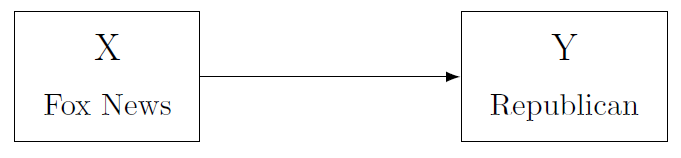
\includegraphics{images/CI/fig2-1.png}
\caption{Our theory: X causes Y}\label{fig:fig2-1}
}
\end{figure}

\begin{enumerate}
\def\labelenumi{\arabic{enumi}.}
\setcounter{enumi}{1}
\tightlist
\item
  Second, we need to think carefully about what is the direction of this
  relationship. Is X "causing" Y, or the other way around? The latter option
  is known as \textbf{reverse causality}, and needs to be considered both when
  you are coming up with your theory and when you are testing your data. Maybe
  Republicans enjoy Fox News more, because the network provides more positive
  coverage of their party than other networks
  (\protect\hyperlink{ref-coeHostileNewsPartisan2008}{Coe et al. 2008}).
\end{enumerate}

\begin{figure}
\hypertarget{fig:fig2-2}{%
\centering
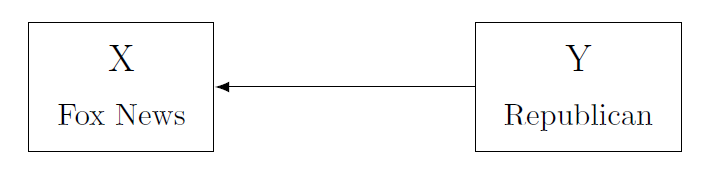
\includegraphics{images/CI/fig2-2.png}
\caption{Reverse causality: Y causes X}\label{fig:fig2-2}
}
\end{figure}

\begin{enumerate}
\def\labelenumi{\arabic{enumi}.}
\setcounter{enumi}{2}
\tightlist
\item
  Third, we need to address the possibility of \textbf{confounding variables}.
  A confounding variable is a variable (Z) which confuses -- i.e.~confounds --
  the observed relationship between X and Y. But since we do not observe this
  variable, we can misinterpret our results. For instance, a variable Z might
  be affecting both X and Y. Yet we are only observing X, so we are not taking
  into account the role that Z is playing in this relationship. This can lead
  us either to erroneously identify a causal link or to erroneously inflate
  the size of the relationship.
\end{enumerate}

In our example, both Fox News viewership (X) and partisanship (Y) could be a
function of age (Z). Old people watch more Fox News, and they are also more
Republican. What we thought is a relationship between watching Fox news and
voting is actually just a reflection of a different set of relationships.

This problem is also referred to as \textbf{omitted variable bias}. You will
learn this in more detail in the chapter on ``Large N'', but the idea is that
you always risk leaving out variables that are key to explaining the causal
relationship, and this can affect your interpretation of results.

\begin{enumerate}
\def\labelenumi{\arabic{enumi}.}
\setcounter{enumi}{3}
\tightlist
\item
  Confounding variables are one possible cause of a specific error called
  \textbf{spuriousness}. A spurious relation is one where X and Y move
  together in the same or opposing direction, yet this movement is being
  driven by a third factor (the confounding variable). A researcher can
  misinterpret this as a causal link between X and Y.
\end{enumerate}

\begin{figure}
\hypertarget{fig:fig2-3}{%
\centering
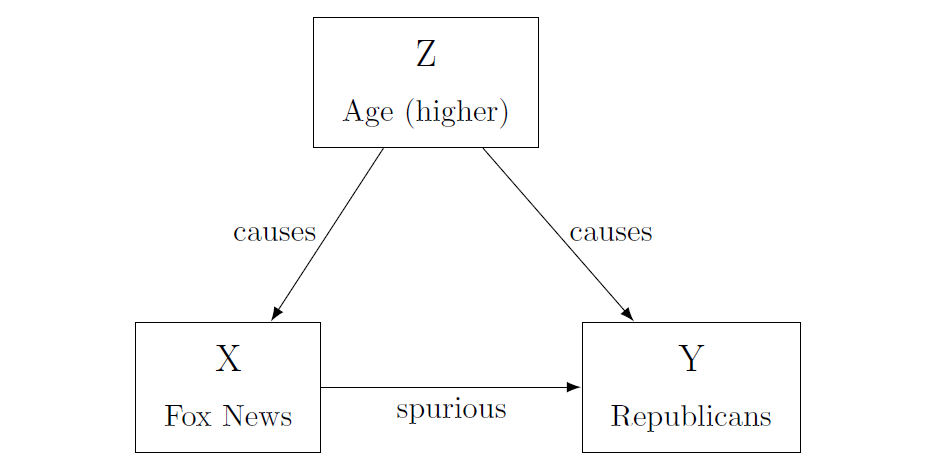
\includegraphics{images/CI/fig2-3.png}
\caption{Omitted Variable: actually, age explains both X and
Y!}\label{fig:fig2-3}
}
\end{figure}

In this case, people who watch more Fox News have higher rates of Republican
support, and those who watch less show lower support: the variables move
together. However, as we just discussed, this movement might be caused by a
third factor. When we take this factor into account, the relationship between
viewership and votes might disappear.

Alternatively, a spurious relationship can simply occur by chance: sometimes
the data just indicate a relationship that is not there in reality. In our
survey of television viewers, we might by simple chance have interviewed a set
of viewers that both watch lots of Fox News and vote Republican, even if this
association does not exist for the general population. If we have done the
sampling well, that is unlikely -- but not impossible.

If we do not watch out for omitted variables, and spuriousness more broadly,
we might claim a causal relationship because of a chance occurrence in the
data or because we have not considered all factors. In practice, this is a
difficult task. It is hard to isolate only one variable, especially when we do
not have measures of every single variable that could also be affecting our
outcome. Actually, in some cases we can't even \emph{think} of all the
possible confounding variables
(\protect\hyperlink{ref-bullockMediationAnalysisHarder2011}{Bullock and Ha
2011, 510})

\begin{enumerate}
\def\labelenumi{\arabic{enumi}.}
\setcounter{enumi}{4}
\tightlist
\item
  Another element to keep in mind when dealing with causality refers to the
  \textbf{causal mechanism}. Can we think of a plausible mechanism linking X
  to Y? Why would viewing more Fox News cause people to vote for Republican
  candidates? Perhaps the channel increases people's knowledge of candidates
  or it may promote certain viewpoints clearly favoring the party.
\end{enumerate}

In any case, having an idea of why two variables are related makes us more
confident that the causal relationship exists.

If we address these questions, then we might have a chance at identifying a
cause-effect relationship. Some methods are better than others at addressing
these issues. Although later chapters will go into more detail on some of
these methodologies, we will briefly introduce them here, focusing
particularly on their strengths and weaknesses towards achieving causal
inference. As mentioned above, causal inference is not restricted to
quantitative methods. Causal relationship can also be revealed through
qualitative methods, such as Process Tracing and Counterfactuals. These tools
rely on in-depth analysis of particular cases by, for instance, examining
historical documents and conducting interviews, and you'll learn more about
them in the chapter on ``Small N''.

\textbf{"Development causes democracy": explain how reverse causality could be operating here.}

\begin{shaded*}

Just as development could cause democracy, it is also plausible that democracy
causes development. For instance, foreign countries and international
organizations could be more willing to provide aid to a democracy than to a
non-democracy. Introducing more freedoms and allowing people to trade and
engage in commerce freely could enhance development as well.

\end{shaded*}

Among quantitative methods, there are two types of methods that try to achieve
causal inference: experimental studies and observational studies. Experimental
studies are the most potent tool for causal inference. Why? Because of
randomization. The essential characteristic that makes experiments so powerful
is the fact that we can randomly assign the treatment (our independent
variable) to our units. Through this seemingly simple action, we are able to
overcome many of the problems mentioned above. Recall that the fundamental
problem of causal inference is that we can never test the counterfactual;
there is no way of holding everything equal except the manipulation of our
independent variable. However, through randomization we can make - on average-
all other things equal across treatment and control group. By randomly
assigning the treatment to units, we can say that the only thing that differs
between the treatment and the control is the presence/absence of the
treatment. This means that these two groups are even similar across variables
we cannot observe, and thus, we are less likely to face a confounding variable
problem.

Although experiments are the preferred tool for causal inference, they are not
always available to use, either because of lack of resources, ethical issues,
or because they are unattainable given our research topic. Experiments are
also most common when dealing with individuals. In cross-country comparisons,
it is practically impossible to carry out experiments.

Very often, we need to take data that is observational in nature and try to
approximate an experiment using more or less complicated statistical
procedures. The term \textbf{observational} comes from the fact that we are
not manipulating the treatment; instead, we are simply observing the data that
was collected. These methods include Difference in Difference, Regression
Discontinuity, Matching, and Instrumental Variables. Explaining these is
beyond the scope of this book but you can find an introduction to them in
(\protect\hyperlink{ref-angristMasteringMetricsPath2015}{Joshua David Angrist
and Pischke 2015}).

Historically, many scholars have made causal claims using simple regressions.
These claims should be approached with caution, as you will learn in more
detail in the chapter on ``Large N''. The way we approximate "all else equal"
with regressions is by controlling for possible confounding variables. We
assume that, once we have controlled for these variables, all that remains is
the cause-effect relationship. Yet, as mentioned earlier, it is practically
impossible to control for all relevant variables. This, and other reasons, are
why some scholars believe that is impossible to make causal claims with
observational data. Indeed, you should be very cautious in concluding causal
relationships from your regression. Notwithstanding, they are a very useful
tool to describe relevant relationships and trends in data.

Finally, it is worth mentioning again that causal inference is not limited to
quantitative work. In the chapter on ``Small N'', you will learn about process
tracing and other approaches that work better for qualitative data and
situations where you have a small number of cases. Some scholars also believe
in the use of both qualitative and quantitative methods within one study,
complementing large-n statistical work with in-depth case work to strengthen
their argument. The interplay between qualitative and quantitative work also
happens at a broader level. Nothing is decided on one study alone. The most
convincing findings in political science are those that have been confirmed by
a variety of scholars using a range of methods.

\textbf{Explain why correlation does not imply causation.}

\begin{shaded*}

When two variables are correlated it means that there is some association
between them: maybe they both increase/decrease at the same time, or they move
in opposite directions at the same time. But this does not mean that the
movement of one variable is causing the movement of the other. For example,
aspirin use is correlated with headaches (aspirin use increases when headaches
appear) but this does not mean that aspirins cause headaches.

\end{shaded*}

\hypertarget{conclusion}{%
\section{Conclusion}\label{conclusion}}

In this chapter we have discussed in broad strokes some of the concerns that
matter when conducting research in political science. The first lesson is
about the importance of the scientific method. Following this framework is the
first thing that separates punditry from political science. Anyone can comment
on politics and offer an explanation on why things are the way they are. Your
job is to scrutinize and analyze facts to come up with empirically based
explanations of reality. The best way to do so is by following the scientific
process: posing a question, engaging with existing theory, hypothesizing
explanations for your puzzle, testing your hypothesis, and interpreting the
evidence.

As has been mentioned throughout the chapter, research goals are varied, yet
we have focused here on one of the most ambitious goals: establishing causal
relationships. Determining a clean relationship between X and Y is not an easy
task. Causality in the social sciences is messy and few times (if ever) is our
outcome caused solely by one variable. So we must deal with the difficulties
of isolating the factor we are interested in, identifying or eliminating all
others that could be standing in the way.

We have stressed the obstacles that stand in the way of causal inference not
to discourage you from attempting it, but for you to be a conscious researcher
and consumer of research. There are still several scholars in the field that
irresponsibly claim to have identified causal relationships when their methods
cannot support such a claim. By having a sense of the challenges behind causal
inference, you can evaluate the validity of these findings. The difference
between good and bad causal research is not primarily in the method used, but
in how careful the researcher has thought about the relationships at hand.
Hopefully this chapter has given you some tools in that regard.

\hypertarget{application-questions}{%
\section{Application Questions}\label{application-questions}}

Imagine you have a research hypothesis: As people become more aware of the
unequal distribution of income in our society, the more they will support a
tax on the wealthy.

\begin{enumerate}
\def\labelenumi{\arabic{enumi}.}
\item
  How would you test this with an experimental study? How would you test it
  with an observational study?
\item
  Perhaps you find that increased awareness of the distribution of income is
  related to less support for a tax on the wealthy. Can you think of any
  confounding variable that could be driving this relationship?
\item
  If you decide to carry out an observational study, what variables should you
  control for? What are possible confounding variables?
\item
  What would the counterfactual in this case look like?
\end{enumerate}

\hypertarget{answers-to-application-questions}{%
\section{Answers to Application
Questions}\label{answers-to-application-questions}}

\begin{enumerate}
\def\labelenumi{\arabic{enumi}.}
\item
  Experiment: randomly assigning people to treatment/control; treatment is a
  video/explanation showing how income is distributed in society; then people
  are asked what they think of the tax. An Observational study: A survey that
  asks people about how they think income is distributed and then asks them if
  they support a tax on the wealthy.
\item
  Maybe those who know how income is distributed are the wealthiest, and they
  are not in favor of being taxed more heavily.
\item
  Education, media consumption, place of residence, race, age.
\item
  A person that knows how income is distributed and then shows level of
  support for tax; then, erasing that person's memory and making the person
  unaware of how income is distributed and asking level of support for tax.
\end{enumerate}

\hypertarget{theory}{%
\chapter{Theory}\label{theory}}

\textbf{By Salih O. Noor}

\hypertarget{introduction-2}{%
\section{Introduction}\label{introduction-2}}

Most people may not know much of anything about theory. Theory is either so
``esoteric and complicated as to be incomprehensible" or "so commonplace and
obvious as to be platitudinous''
(\protect\hyperlink{ref-shoemakerHowBuildSocial2003}{Shoemaker, Jr, and
Lasorsa 2003, 5--6}). Either way, to most people, theories seem to be of
little use. In reality, however, people use theories every day about
friendship, dating, success, and so on. Political scientists rely on theory to
analyze public opinion or predict election results, and weather analysts apply
theory to forecast weather conditions. Most people, however, misunderstand
what a theory is and what a theory does.

In this chapter we will study the meaning, significance, and building blocks
of theory as well as theory-building and theory testing procedures. In the
second section, we will discuss what theory is and is not, and how empirical
theory differs from other kinds of claims or theories in its application of
the scientific method. In the third section, we will learn some
characteristics that define a good theory, discussing four very important
elements of a well-crafted theory. In the fourth section, we will try to
understand literature review and its importance to theory. In the last
section, we will study the relationship and differences between
theory-building and theory-testing, in addition to inductive and deductive
reasoning and procedures in theory-building. For elaboration, we will draw at
all stages on various examples from the social (and when necessary the
natural) sciences, including two check boxes on the scientific method and on
examples in theory-building and testing.

\hypertarget{what-is-a-theory}{%
\section{What is a theory?}\label{what-is-a-theory}}

A \emph{scientific theory} is a set of logically consistent statements that
tell us why the empirical social and political phenomena we observe, or the
relationships between them, occur in the way they occur. More formally, a
theory ``is a system of constructs (concepts) and propositions (relationships
between those constructs) that collectively present a logical, systematic, and
coherent explanation of a phenomenon of interest within some assumptions and
boundary conditions''
(\protect\hyperlink{ref-bacharachOrganizationalTheoriesCriteria}{Bacharach
1989, 496}). In short, a theory is an interrelated set of propositions about
empirical reality. These propositions are comprised of (1) concepts that
introduce basic terms of the theory; (2) assumptions that relate the basic
concepts to each other; and (3) generalizations that relate the statements to
a set of observations or, simply, report the findings on observed
relationships. It is important that these propositions are ``logically
consistent'' in that they must all be true at the same time; the theoretical
concepts, assumptions, statements should be coherent with each other.
Concepts, variables, and hypothesis are the building blocks of theory.

For example, the ``logic of collective action'' is a theory that aims to
explain the dilemma of collective action and public goods. Formulated by
political scientist Mancur Olson, Jr.
(\protect\hyperlink{ref-olsonLogicCollectiveAction2003}{Olson 1965}), the
theory explains when (and why) do some collective groups (such as trade
unions, social movements, or college students) organize better to achieve
public goods (like increased wage, policy change, or improved campus security)
than other groups. Olson found that the interests of highly coherent minority
groups can be overrepresented, and the interests of majorities get
marginalized due to the ``free-rider'' problem. Collective action is difficult
because individual members always have incentives to "free ride" on the
efforts of others, because ``public goods'' --- goods or services that are
available to every member --- are by definition non-excludable (i.e.~one
member cannot reasonably prevent another from consuming them) and
non-rivalrous (i.e.~one person's consumption of the good does not affect the
others' chances). As a result, some members (e.g.~workers) can expect to enjoy
public goods, such as increased wages and improved workplace conditions
without bearing the costs of participating in a strike (e.g.~time, money, or
physical harm). In particular, large groups face tremendous challenges for
collective action than small groups, because individuals in large groups gain
less per capita of a successful collective action due to diminishing returns.
On the contrary, small groups can provide selective incentives to their
members and a prospect of greater rewards for each a successful collective
action due to small number of members. As a result, Olson concludes, it is
highly possible that a minority group bound together by concentrated selective
incentives can dominate a majority social group. In so observing, Olson
refuted previous theories that held (a) individuals in a group (of any size)
will act collectively to achieve their common interests, and (b) the greatest
threat in a democracy is, due to the majority's sheer numbers, ``the tyranny
of the majority''.

A theory should \emph{explain} why things happen, rather than just describe or
predict. It is entirely possible to predict events or behaviors using a set of
predictors, without necessarily explaining why such events are taking place or
why they take place together. For instance, stock market analysts predict
fluctuations in the stock market based on market announcements, earnings
reports of major companies, and/or new data from the Federal Reserve, based on
previously observed correlations. In contrast, theoretical explanations
require causation, or the understanding of cause-effect relationships.
Establishing causation requires four conditions: (1) correlations between two
concepts, (2) temporal sequence (the cause must precede the effect in time),
(3) causal pathway (causal mechanism that link cause to effect), and (4)
rejection of alternative hypotheses through testing
(\protect\hyperlink{ref-bacharachOrganizationalTheoriesCriteria}{Bacharach
1989, 496--515})

Theoretical explanations can be \emph{idiographic} or \emph{nomothetic} that
vary in their theoretical premise and explanatory scope. Idiographic
explanations are those that explain a single situation or event, say
unemployment in the state of Illinois, in idiosyncratic detail. The
explanation is detailed, accurate, and valid, but it may not apply to other
similar situations, say other states, and is hence not broadly generalizable.
In contrast, nomothetic explanations seek to explain a class of situations or
events, for example unemployment in several US state, rather than a specific
situation or event. Because nomothetic explanations are designed to be
generalizable across contexts (events, or people, countries), they nonetheless
tend to be less precise, less complete, and less detailed. As such,
idiographic and nomothetic explanations rely on different assumptions of
causality, different analytical tools, and different approaches to
theory-building. Methodologically speaking, therefore, the two approaches to
social science theory often fall along the qualitative-quantitative divide;
the first typically uses small-N methods of analysis (e.g.~cross-case
analysis, within-case analysis or process tracing, and set theory) for one or
few number of cases, while the second applies large-N methods of quantitative
analysis (e.g.~large-scale surveys, statistical analysis, regression) to a
large number of cases. Further on these methods, read the chapters on
\href{/small-n.html}{small-N} and \href{/large-n.html}{large-N} analysis.

Theories are important in the social and political sciences. They help us,
among other things, to understand the nature of political and social phenomena
(such as political events, behavior, institutions, and processes), to explain
observed regularities among these phenomena (i.e.~causal relationships between
events or processes), to make predictions about as yet unobserved
relationships (e.g.~the possible effect of immigration policy on the 2020 US
presidential elections), and to take a particular policy action
(e.g.~universal healthcare to reduce high healthcare costs). Without theories
it is hard to have valid knowledge of political events, behavior, and
processes, or tools to understand the relationships between different
political events and processes.

However, theories can also have their own share of (systematic or
non-systematic) limitations. As simplified explanations of reality, theories
may not always provide adequate explanations of the phenomenon of interest.
While social reality is often more complex, theories are designed to be simple
and parsimonious explanations based on a limited set of concepts/variables and
concept/variable-relationships. Furthermore, theories may impose cognitive
blinders or limit researchers' ``range of vision,'' causing them to miss out
on important concepts that are not identified by the theory (i.e.~omitted
variable). The nature of these limitations sharply vary between small-N and
large-N theories, with the strengths of one being the limitations of the
other.

For a better understanding of what theory is, it is good to think in terms of
what theory is not. First and foremost, the theory -- i.e.~\emph{empirical
theory} -- we are concerned with here, such as Olson's ``logic of collective
action,'' is epistemologically different from normative \emph{political
theory} in political or general philosophy. Empirical theory is concerned with
the examination of empirical political and policy matters through the
scientific assessment of empirical evidence rather than, as political theory,
with the realm of political ideas, values, and norms from a normative
perspective. The latter is typically concerned with questions of overtly
normative nature, such as: What system of government best guarantees freedom,
justice, and equality in society?; When is obedience to a ruling power
justified, and when is disobedience not justified?; Or how citizens ought to
behave towards their rulers or the state? Empirical social theory rather
inquires, for example, how and why a particular political system
(e.g.~democracy, dictatorship, military regime) emerges, why citizens behave
in a particular way towards their government or leaders, or what caused voters
to support the Democratic Party over the Republican Party in the 2016 U.S.
Presidential Elections. The latter also differs from normative theory in terms
of the tools, methods, and techniques applied in answering questions about the
social and political world around us.

Social science theories are generated through the application of the
\emph{scientific method} -- or the principles and procedures of interpreting
the empirical world through objective, value-neutral observation of facts. Put
simply, the scientific method is a process of guessing and verifying to reach
descriptive or causal explanations---i.e.~making assumptions/ hypotheses about
the real social/political world, examining evidence (data) gathered from that
world, and confirming (or disconfirming) those hypotheses in view of the
evidence. Even though there is no social scientific method clearly written
down that is followed by all scientists, it is possible to identify five steps
associated with the method:

\begin{enumerate}
\def\labelenumi{\arabic{enumi}.}
\item
  Formulate a \textbf{question} after observing a social/political puzzle;
\item
  Develop a \textbf{theoretical model/framework} to explain it;
\item
  Propose a \textbf{hypothesis/testable implication};
\item
  \textbf{Test hypotheses} against evidence; and
\item
  \textbf{Confirm/reject} the hypothesis after analyzing the evidence.
\end{enumerate}

The scientific method stipulates clear and logical steps (Checkbox 1) that
must be strictly followed in our search for explanations. Social scientists
develop theories through the formulation of a question, proposing hypotheses
about what they think the answers are, testing the hypothesis against evidence
collected and examined in an objective and systematic manner, and drawing
theoretical conclusions that are falsifiable through the iterative application
of the scientific procedures. Therefore, empirical theory is different from
normative political theory in that the latter relies on tools other than the
scientific method to deal with normative and ethical questions. Normative
questions ask for a normative response, seeking an indication of what is good
or of what should be done; ultimately, the answers involve what someone likes
or dislikes, values or rejects. The scientific method cannot provide the
answers without regard for an individual's personal values or preferences.

\textbf{Checkbox 1: The Social Scientific Method}

\begin{itemize}
\item
  STEP1: Research Question,The first step in the scientific method is to
  observe the world and come up with a question. The very need for a theory
  begins when we observe something that is so puzzling that we ask ``why did
  it occur?'' or ``what caused it to occur?'' What makes the observation a
  puzzle worth exploring is that the observation does not fit with some prior
  expectation or theory that we held to be true about how the world works.
  Therefore, we always have a preexisting theory or expectation when we
  observe the world that leads to a new puzzle or question.
\item
  STEP 2: Theory or model The next step after observing something puzzling is
  to develop a theory (also sometimes called theoretical framework or model)
  to explain it. This is a set of logically consistent statements that tell us
  why the things that we observe occur in the way they do. The task here is to
  propose an explanation for the phenomenon the researcher is interested in
  understanding. Developing a theory requires imagination and creativity to
  fathom the social world, to impose some analytical order on an otherwise
  complex world. In short, the model will be a simplified picture of the
  world; it will be something that helps us understand some relationships
  between two or more empirical phenomena. A good model, therefore, contains
  only what is needed to explain the phenomenon that puzzles us and nothing
  else. At times, this step involves developing a theoretical framework or
  structure that can hold or support the theory. A theoretical framework
  consists of concepts, variables, and the theoretical assumptions of the
  theory that explains the problem under study. It is the conceptual basis for
  understanding, analyzing, and designing ways to investigate relationships
  within social systems.\\
\item
  STEP 3: Hypothesis (Implications) Once we have a model, the third step in
  the scientific method is to deduce implications from the model. Our model
  will presumably provide a logical explanation for the puzzling observation
  that we started with; after all that is what it was designed for. To
  actually test the model and allow for the possibility that it can be
  falsified, we will have to find other implications that can be deduced from
  it. We must ask ``If the prior world that we created to explain the
  phenomena that we originally found puzzling really did exist, what else
  ought to exist? What else should we be able to observe?'' Good models are
  those that produce many different implications because each prediction
  represents another opportunity for the model to fail and, thereof, makes the
  model easier to falsify. If the model fails to be falsified, we gain more
  confidence in its usefulness. Good models also produce small surprising
  implication --i.e.~they tell us something we would no know without the
  model. Models are not particularly useful if they tell us only what we
  already know.\\
\item
  STEP 4: Test Hypotheses The fourth step is to examine whether the
  implications of the model are consistent with observation. We should not
  dogmatically uphold the implications of our model or defend them to prove
  they are right. On the contrary, we should try our best to falsify them
  because it is only after a theory has withstood these attempts that we can
  reasonably have confidence in it. Testing the implications that are most
  likely to be falsified is particularly important. Always subject a model to
  the harshest test that you can devise. It is also standard to ask if other
  (existing) models might also explain the phenomena of interest. In this
  case, the researcher should compare the implications of those other models
  with the implications of her own model. It is always the case that competing
  models have some of the same implications, yet they will differ in some
  other implications (otherwise they are not different models). The trick is
  to identify these points of conflict between the different models and the
  relevant observations in the real world that would help decide between them.
  This --called critical test -- allows the analyst to use observation to
  distinguish between two or more competing explanations of the same
  phenomenon. After all there is only one world and only one of the models can
  be consistent with the real world.
\item
  STEP 5: Evaluation Confirmation or refutation of the theory is the last step
  in the scientific method. Our theory has been confirmed if we observe the
  implications deduced from our theory. Note that we cannot say our theory has
  been verified or proven because we can never prove or disprove a scientific
  explanation. Scientific method is a means to ``provisionally'' understand
  the world, and scientific theories serve as provisional explanations of the
  world contingent on better methods, better analytical tools, and better
  evidence. Our theory may or may not be true. All we can conclude, if the
  observations are consistent with our theoretical implications, is that our
  theory has not yet been falsified. We cannot rule out the possibility that
  it can be falsified the next time it is tested.
  (\protect\hyperlink{ref-clark2017principles}{Clark, Golder, and Golder
  2017})
\end{itemize}

Second, a theory is not the same as a \emph{model} or paradigm. Theory and
model are related terms and not infrequently confused. But the two are
different from each other in their definition, purpose, and application.
First, as defined above, theory is a conceptual framework or general
explanation of an idea. A model (not the same as theoretical model) by
contrast is a verbal or a visual representation of a concept in order to make
the understanding of something easier and clearer. Second, the purpose of a
theory is to explain things and is less practical, whereas a model is meant to
simplify things and is more practical. The social and political world is
immensely complex; models present a simplified picture of the world that
puzzles us. Models present in simple and concise manner concepts, assumptions,
and claims, which are the building blocks of theory. Models are commonly used
in all political science, but game-theoretic models in rational-choice
approaches represent the most popular forms of modelling the behavior and
actions of rational actors like voters, politicians, special interest groups,
and states. For example, in Olson's theory of collective action individuals
are modelled as rational, interest-maximizing actors who act only under
circumstances that maximize their interests. This simple model illustrates an
otherwise complex social and mental reality of actors interacting in large
group contexts. Therefore, theory and model coexist in the same world of
social science inquiry, yet they differ, and the failure to realize this
difference can lead to confusion and perhaps in disillusionment. Theories
should be understood as explanations or conclusions about certain situations
or problems, while models as heuristic devices that help us understand,
through concepts and theories, how some aspects of the world work and explain
it to others. Models, therefore, can represent a theory but they cannot be a
substitute for theory.\\
Read (\protect\hyperlink{ref-shoemakerHowBuildSocial2003}{Shoemaker, Jr, and
Lasorsa 2003}), chapter 7, for a greater discussion of theory versus model,
and (\protect\hyperlink{ref-clarkPrinciplesComparativePolitics2013}{Clark,
Golder, and Golder 2013}), pages 121-137, for examples of game-theoretic
models.

Third, a theory is not a \emph{paradigm}. A paradigm is a broad, general
framework or approach that defines a particular scientific discipline. It is a
distinct set of concepts and assumptions, including theories, research
methods, postulates, and standards that guide scientific inquiry in a
particular community of scholars. It determines the kind of questions supposed
to be asked and their structure, the assumptions made, the methods used, and
how the results should be interpreted
(\protect\hyperlink{ref-kuhnStructureScientificRevolutions1996}{Kuhn 1996,
10}). Scientific paradigms set the standards for studying the empirical world,
while theories are explanations of some aspects of that world. In addition,
unlike theory, a paradigm is not actually testable per se. Examples of
paradigms in political science include systems theory, rational choice theory,
comparative historical analysis, neo-liberal institutionalism, and
constructivism.

Fourth, and last, social scientific theories are general explanations, and not
``covering laws'' of political and social behavior. It is possible to have
law-like theories in the natural sciences with universal applicability to all
natural phenomena; theories of electromagnetism, evolution, and relativity are
some examples. This because natural phenomena display behavior and (causal)
regularities that are uniform across time or space. For example, water boils
at 100 degree centigrade almost always whereas, according to Albert Einstein,
light travels at a speed of 186,000 miles/second, and is unchanging. As Max
Weber argued, the laws that regulate social relations are quite different from
the laws that govern nature; regularities in human behavior and the physical
world are fundamentally different because the former display a great degree of
irregularity, fluidity, and heterogeneity. Unlike natural events, political
events and processes do not lend themselves to the same explanatory logic as
is found in physics and the other hard sciences.

This is to neither say that human behavior is devoid of regularities nor
law-like generalizations to explain it are entirely impossible. It is not rare
that social scientists seek to identify such regularities and develop general
explanations; examples include: Duverger's law of plurality voting and
two-party system
(\protect\hyperlink{ref-duvergerPoliticalPartiesTheir1954}{Duverger 1954}),
modernization theory on modernization and democracy
(\protect\hyperlink{ref-lipsetSocialRequisitesDemocracy1959}{Lipset 1959});
and Moore's ``No bourgeoisie no democracy'' hypothesis on the middle class and
democracy (\protect\hyperlink{ref-mooreSocialOriginsDictatorship1966}{Moore
1966}). These theories validly explained a broad range of historical
observations, but their applicability turned out to be limited to a particular
context---i.e.~mostly advanced Western democracies before mid-twentieth
century---which signifies that the utility of social scientific theories is
context- and time-specific because regularities in human behavior hinge on the
given cultural, political, and economic context. Most social scientists aspire
to produce generalizations about the world; in fact, a central goal of
scientific analysis is to generate concepts, models, and theories that travel
across time and space. However, social and political phenomena are
characterized by complexity, randomness, and diversity to yield themselves to
law-like, universal theories. Cause and effect greatly vary across countries,
cultures, regions, and historical contexts. What obtains to observations in a
specific context often does not apply to other observations in a different
context. The demise of modernization theory after the 1960s was precisely
because education, urbanization, and industrialization (i.e.~modernization) in
the Third World did not cause democracy but instability, revolutions and
dictatorships. Moreover, the more general a theory is (i.e.~it explains too
many observations), the less is its explanatory power concerning each
observation. In fact, a social science theory that explains everything does
not explain anything. Due to the complexity of causality, therefore, social
science theories are judged less by their universal applicability than by
their validity and robustness in explaining a particular set of observations.
Theoretical generality and specificity are two competing goals in
theory-building, with large-N (quantitative) analysis associated with the
former and small-N (qualitative) with the latter.

\hypertarget{what-is-a-good-theory}{%
\section{\texorpdfstring{What is a \emph{good}
theory?}{What is a good theory?}}\label{what-is-a-good-theory}}

A good theory should explain previously puzzling facts, be logically
consistent, and produce potentially falsifiable predictions. It builds on
existing theories, has clearly specified concepts (valid conceptualization)
codified as measurable variables (valid measurement), and clearly shows the
relationship between the concepts (causal pathway). Even though the standards
for a good theory are debatable, particularly among qualitative and
quantitative traditions, social scientists agree on some basic elements of
what makes a good theory. We will discuss here four major characteristics of a
good theory.

\emph{Parsimony} is the first such element. How simple is the explanation? The
simplest theory (i.e.~one that uses the smallest number of variable or makes
the fewest assumptions) is considered the best. A theory is considered as
parsimonious when it has the ability to explain often complex phenomena in
relatively few terms and statements. A parsimonious theory can specify the
causal relationship (X---\textgreater Y) in clear terms using a causal model
(which might involve multiple variables and relationships) that reasonably
simplifies a complex empirical reality in to something comprehensible.

The second feature is \emph{generalizability} or theoretical coverage. A good
theory is generalizable when it has the power to explain a broad range of
similar cases or phenomena outside the context of that study. In other words,
the conclusions of a scientific theory are applicable to other contexts not
included in the study, which is also referred to as the external validity of a
theory. In qualitative research, this criterion is less important because
theory is generated from a small set of cases and is less applicable to other
contexts. Qualitative analysis rather puts greater emphasis on the internal
validity of a study or the extent to which the theoretical claims are based on
valid methods of analysis and evidence about cause and effect. Theoretical
claims or inferences possess internal validity if claims of a causal
relationship between two variables demonstrate that the "cause" occurrence
before the "effect" (temporal precedence), the "cause" and the "effect" tend
to occur together (covariation), and there are no alternative channels or
mechanisms that explain the observed variation (nonspuriousness).

\emph{Observable implications} or the ability of a theory to help make more
accurate predictions about new unobserved instances is the third quality of a
good theory. Strong theories have strong observable implications or the things
we would expect to observe in the real world if our theory is right. For
example, the preference theory of judges states that judges want the law to
reflect their ideological preferences; and, because they lack an electoral
connection, they are free to vote in accord with their ideological
preferences. If this theory is correct, we should observe judges generally
voting in accord with their ideological preferences, such that conservative
judges cast conservative votes and liberals, liberal votes.

The fourth and last criterion used to judge a social scientific theory is
\emph{falsifiability} or its refutability. A good theory must be falsifiable
or liable to refutation when subjected to tests using new observations or new
evidence; it must be possible to identify a possible outcome of test or
observation that conflicts with predictions of a given theory. In fact,
according to the philosopher of science Karl Popper who introduced the concept
as the basic principle of scientific inquiry, statements and theories that are
not falsifiable are unscientific or not based on the scientific method. The
most common way in the social sciences to support falsifiability (or safeguard
against invalid refutation of a theory) is to specify the scope conditions or
assumptions under which a theory is applicable. Scope conditions are
parameters or boundaries specified by the analyst that identify the types of
empirical contexts or observations to which the theory applies. For example,
we can state that the preference theory of judges is applicable under the
condition that judges vote in accordance with their ideological preferences
only in the absence of a liberal (i.e., a potential whistle-blower) on the
panel. The theory may be falsified when we observe that, say, conservative
judges fail to cast conservative votes even in the absence of a potential
whistle-blower.

\hypertarget{literature-reviews-and-theory}{%
\section{Literature Reviews and Theory}\label{literature-reviews-and-theory}}

We noted in the first section that developing an explanation begins with a
puzzle and a research question. The first major task in a research effort
often is to find a puzzling topic and to translate a general interest in a
topic into a manageable research question or series of questions. Framing an
engaging and appropriate research question will get a research project off to
a good start by defining, and limiting, the scope of the investigation while a
poorly specified question inevitably leads to wasted time and energy. But most
students, when confronting a research project for the first time, either do
not have a well-formulated research question as their starting point or any
specific interest or topic in mind at all. We may also not know whether
explanations, that fully or partially address the puzzle we have observed,
already exist. To address these challenges the first major task is to conduct
a literature review; i.e.~to examine systematically scholarly literature that
is relevant to the puzzle. Why is this important? How does thoroughly studying
extant literature contribute to theory?

A literature review is a survey of books, scholarly articles, and other
sources relevant to a particular issue, area of research, or theory, and by so
doing, provides a description, summary, and critical evaluation of these works
in relation to the research problem at hand. It is designed to provide an
overview of sources you have explored while surveying a particular topic and
to demonstrate to your readers how your research fits within a larger field of
study (\protect\hyperlink{ref-finkConductingResearchLiterature2013}{Fink 2013,
5}). Good research involves reviewing previous work to motivate and sharpen a
research question. Reviewing relevant literature also contributes to theory
development for several other reasons. Among these are: (1) to gauge what has
and has not been studied, (2) to develop general explanations for observed
variations in a behavior or a phenomenon, (3) to identify potential
relationships between concepts and to find hypotheses, (4) to learn how others
have defined and measured key concepts, (5) to identify data sources that
other researchers have used, and (6) to develop alternative research designs.
Lets further discuss some of the reasons that are more crucial to theory
development.

Often times, a researcher or student will start off by expressing only a
general interest in a topic, such as gun violence or the effects of campaign
advertising, but the specific research question has yet to be formulated; for
example, ``What is the social background of individuals who engage in mass
shooting?'' or ``Do negative TV campaign advertisements sway voters?'' A
review of previous research on these topics can help you carve a research
topic by identifying research questions that others have addressed.

A researchers, on the other hand, may start with an overly specific research
question such as "Do evangelicals have different views on abortion policy than
non-evangelicals?" Reading the literature on public opinion on abortion will
likely reveal that your specific research question is one of many aimed at
answering the more general research question: What are the social attributes
of people who are opposed to abortion, and do they differ from those who
support abortion access? Compared to the former question, which is too narrow
to sustain a research paper, the latter research question constitutes a topic
that is likely to lead to theoretically crucial conclusions and more
observable implications.

A literature review also can help you to identify gaps or analytical
shortcomings in the literature. Here, you may find that, after reading the
scholarly work in an area, previous research does not adequately answer the
question for lack of effective research tools, sufficient data, and/or
appropriate theoretical approach. You may design a new research project to
answer an old question in a novel way using new data. A study may also
replicate a previous study to confirm or challenge a hypothesis or expand our
understanding of a concept. Replication is one of the cornerstones of
scientific work; by testing the same hypothesis through different research
design or confirming the results from previous research using the same data
and methods, we can increase our confidence that the results are valid.

At other times, a researcher may begin with a hypothesis to develop an
explanation for a relationship that has already been observed. Here, a
literature review may reveal similar observations made by others previously
and may also help you develop general explanations for the relationship by
identifying theories that explain the phenomenon of interest. Your research
will be more valuable if you can provide a general explanation of the observed
or hypothesized relationship rather than simply a report of the empirical
verification of a relationship.

A researcher, on the other hand, should be alert for competing or alternative
hypotheses rather than just seeking theories that support the plausibility of
own hypothesis. Here, you may start with a hypothesis specifying a simple
relationship between two variables. Since it is rare for one political
phenomenon to be related to or caused by just one other factor or variable
(i.e.~causal complexity), it is important to look for other possible causes or
correlates of the dependent variable (i.e.~omitted variable). Data collection
should include measurement of these other relevant variables so that you may
rule out competing hypotheses or at least specify more clearly the nature of
the relationship between the variables
(\protect\hyperlink{ref-johnsonPoliticalScienceResearch2016}{Johnson,
Reynolds, and Mycoff 2016, 82--84}).

A thorough understanding of existing scholarly work, therefore, is key to
formulate an interesting question, test an existing hypothesis or craft new
hypotheses, and the development of scientifically valid and useful
explanations. Developing skills to understand key concepts and models in the
subfield, to critically evaluate and synthesize expert knowledge, and to
summarize complex arguments in often a large body of literature are essential
for an excellent literature review. Furthermore, personal insight and
non-scholarly sources (e.g.~newspapers, broadcast media, internet) can be
quite helpful in selecting a research topic, and a literature review can
encompass virtually anything published on your topic. However, at the very
least familiarity with the scholarly literature is strongly encouraged.
Relying on scholarly rather than non-scholarly sources greatly improves the
quality of a literature review. After all, a literature review is supposed to
assess the knowledge about a topic that has been attained and communicated
according to scientific principles. Finally, how many books and articles is
one supposed to review depends on the purpose and scope of the project, as
well as source availability. Obviously, a more complex research topic, or a
subject with a larger literature, may require a more in-depth literature
review than will a less complex topic or one with a smaller literature.
Further readings on: the importance of literature review
(\protect\hyperlink{ref-johnsonPoliticalScienceResearch2016}{Johnson,
Reynolds, and Mycoff 2016};
\protect\hyperlink{ref-finkConductingResearchLiterature2013}{Fink 2013};
\protect\hyperlink{ref-hartDoingLiteratureReview1998}{Hart 1998};
\protect\hyperlink{ref-ridleyLiteratureReviewStepbyStep2012}{Ridley 2012};
\protect\hyperlink{ref-knopfDoingLiteratureReview2006}{Knopf 2006};
\protect\hyperlink{ref-jessonDoingYourLiterature2011}{Jesson, Matheson, and
Lacey 2011}) and structure and writing techniques
(\protect\hyperlink{ref-cookLiteratureReviewSkills2014}{Cook and Murowchick
2014}; \protect\hyperlink{ref-finkConductingResearchLiterature2013}{Fink
2013}; \protect\hyperlink{ref-hartDoingLiteratureReview1998}{Hart 1998};
\protect\hyperlink{ref-jessonDoingYourLiterature2011}{Jesson, Matheson, and
Lacey 2011};
\protect\hyperlink{ref-onwuegbuzieSevenStepsComprehensive2016}{Onwuegbuzie and
Frels 2016};
\protect\hyperlink{ref-ridleyLiteratureReviewStepbyStep2012}{Ridley 2012};
\protect\hyperlink{ref-boothSystematicApproachesSuccessful2016}{Booth, Sutton,
and Papaioannou 2016}).

\hypertarget{theory-building-vs-theory-testing}{%
\section{Theory-building vs Theory
testing}\label{theory-building-vs-theory-testing}}

Social scientific research may involve many activities such as interpretation
of constructs or concepts, describing a social phenomenon (descriptive
inference), and identifying links between two or more related phenomenon
(causal inference). But the two core activities and goals that underlie most
activities (in causal inference in particular) are theory-building and theory
testing. Both are interrelated scientific endeavors that apply the scientific
method, but they vary in important respects that should be properly
understood. As table 1 summarizes, they vary in terms of their epistemological
approach, main goals and tasks, and end results. At the end of section, we
will discuss three exemplary theory-building and theory testing works in the
political science for elaboration; but in the meantime, we will use natural
science examples to easily highlight -- for the latter are relatively
straightforwardness -- the differences between the two.

\begin{longtable}[]{@{}
  >{\raggedright\arraybackslash}p{(\columnwidth - 4\tabcolsep) * \real{0.1538}}
  >{\raggedright\arraybackslash}p{(\columnwidth - 4\tabcolsep) * \real{0.5128}}
  >{\raggedright\arraybackslash}p{(\columnwidth - 4\tabcolsep) * \real{0.2692}}@{}}
\toprule
\begin{minipage}[b]{\linewidth}\raggedright
\end{minipage} & \begin{minipage}[b]{\linewidth}\raggedright
Theory building
\end{minipage} & \begin{minipage}[b]{\linewidth}\raggedright
Theory testing
\end{minipage} \\
\midrule
\endhead
Main approach & Inductive reasoning & Deductive reasoning \\
Research goal & Estimating a relationship/ offer an explanation & Evaluating
an explanation/ test existing hypothesis \\
Main task & Developing hypothesis; test hypothesis against evidence & Finding
evidence to test existing hypothesis \\
Outcome & New or modified theory offering new explanation & Old theory
confirmed or refuted \\
\bottomrule
\end{longtable}

\textbf{Table 1: Theory-building and theory testing compared}

Theory testing, as the phrase suggests, is the process of testing (verifying)
whether a certain theory is a plausible explanation of a phenomenon you would
like to investigate. Its goal is to test the validity of an explanation often,
but not always, through a research design, new data, and/or data analysis
tools. The main focus of theory testing is to discover whether there is
evidence that supports (or does not support) a particular theory. Theory
testing is relatively easier than theory building. While researchers (scholars
and post-graduate students) undertake a much more challenging research task of
theory building, students often do research primarily aimed towards theory
testing. Still, though, it is critical to deeply understand the theory and how
it is used to frame empirical research before you can adequately test it
yourself.

To clarify theory testing, take the Anthropogenic Global Warming (AGW) Theory,
which asserts that human-caused greenhouse gas emissions are the main cause
for the rising global warming levels observed in recent years. Carbon dioxide
comprises one of the greenhouse gasses. Carbon dioxide causes water on the
surface of the earth to evaporate; increased water vapor in the atmosphere in
turn can trap heat coming from the earth thus cause global warming. To test
this theory, the first step is to look into the humidity levels associated
with carbon dioxide emissions because the theory posits that carbon dioxide
causes water to evaporate and trap heat. Greater carbon dioxide means greater
water vapor in the atmosphere measured using, say, a wet and dry bulb
thermometer. The next step is to find out if there is a correlation between
surface humidity and temperature, which should be positive for the theory to
be true. The main task of theory testing is thus to find evidence to confirm
or refute a theory.If the evidence supports the theory, then no further action
is required. If the evidence rejects the theory then you can conclude either
the theory is incorrect or the data is inadequate.

Theory building by contrast is an attempt to explain something as yet obscure
do novo or in different perspective than has previously been suggested. The
goal of theory-building is to provide a framework for analysis to better
understand puzzling empirical issues and to help address real world problems.
As such, it requires knowledge of the plausible theories explaining the
phenomenon currently are, and how they are used in empirical research. Theory
building demands the application of higher-level thinking skills compared to
theory testing. It requires the synthesis of a broad range of literature,
concept formation, the formulation of testable hypotheses, the collection and
systematic analysis of data, and evidence-based confirmation or refutation of
the hypothesized relationships between cause and effect. To be sure,
theory-building can also take place by extending or modifying existing
theories to new contexts. Here, a researcher attempts to replicate and/or
reexamine previously theorized relationships, identifies new causal mechanisms
(or pathways), uncovers previously unexplored relationships between variables,
and introduces a new concept (or significantly re-conceptualizes an existing
one).

In general, there are four major ways of theory-building:

\begin{enumerate}
\def\labelenumi{\arabic{enumi}.}
\item
  Grounded theory-building: building theory inductively based on observed
  patterns of events of behavior in one or few more cases.
\item
  Conceptual analysis: building theory inductively by conducting a bottom-up
  conceptual analysis to identify different sets of predictors relevant to
  phenomenon of interest using a predefined framework. In one such framework,
  a researcher looks for different categories of inputs (factors) related to
  the output (effect), and explain the underlying process that links the two
  categories or concepts.
\item
  Extend/modify existing theory: building theory deductively by extending or
  reformulating existing theories to explain a new context.
\item
  Apply existing theory in new context: building theory deductively by
  applying theories developed in one context to an entirely new context by
  drawing up on the structural similarities between the two contexts.
\end{enumerate}

To further clarify the idea of theory building, let's now consider another
example from the hard sciences. To this day, scientists debate what caused the
sudden extinction of dinosaurs in what is known as the Cretaceous-Tertiary
extinction event, or the K-T event, at approximately 66 million years ago. The
leading hypotheses predicted that a giant volcano, sudden cooling down of
earth climate, and an asteroid strike was the cause. In the early 1980s,
father-and-son scientists Luis and Walter Alvarez suddenly discovered (in
Italy) a distinct thin layer of iridium--an element found in abundance only in
space--that corresponds to the precise time the dinosaurs died. The
researchers deduced that the thin layer of iridium at the K-T boundary was
deposited following the impact of a large meteor, comet or asteroid with the
earth. Furthermore, this bolide impact (the meteor, comet or asteroid
colliding with the earth's surface) could have caused the extinction of the
dinosaurs. However, conclusive evidence -- especially evidence of the meteor,
comet or asteroid collision with earth -- was required to support the theory
and to eliminate rival hypotheses. Then, in the 1990s, scientists discovered a
massive meteor crater (the Chicxulub Crater), 110 miles in diameter, on the
edge of the Yucatán Peninsula, extending into the Gulf of Mexico, which dates
to the period in question. Scientists concluded that the 6-mile-diameter
bolide that formed the crater struck the earth at 40,000 miles per hour and
released 2 million times more energy than the most powerful nuclear bomb ever
detonated. The resulting darkness could have plunged the earth's temperatures
into the freezing zone, killing some three-quarters of the plant and animal
species on Earth, including dinosaurs, within weeks.

Scientists reached the above conclusion through inductive reasoning
--i.e.~they used a small piece of evidence (iridium) about a specific
observation to reach a more general conclusion. Inductive and deductive
analysis -- analytical approaches discussed in the previous chapter -- play
different roles in theory-building and theory testing. The inductive approach
(inductive-statistical) is often associated with theory development. t's a
grounded theory-building approach whereby a researcher makes a detailed
observation of a case or few cases, to derive broad generalizations and ideas
that apply to a broader set of similar cases. Characteristic of qualitative
small-N analysis, this approach aims to generate meanings from the data set
collected in order to identify patterns and relationships to build a theory.
Patterns, resemblances, and regularities are observed in order to reach
conclusions (or to generate theory). The deductive (hypothetico-deductive)
approach is most often useful in theory testing. Characteristic of
quantitative large-N analysis, in deductive analysis a researcher begins with
a theory, then conducts research in order to test whether that theory or
hypothesis is supported by specific evidence. Extending or modifying an
existing theory to fit new reality is a deductive exercise in theory testing.

Whether one applies inductive or deductive analysis, theory-building involves
a series of steps from the identification and definition of concepts to the
expression of their relationship in a theoretical statement, the construction
of a rationale, and the specification of measurements
(\protect\hyperlink{ref-shoemakerHowBuildSocial2003}{Shoemaker, Jr, and
Lasorsa 2003}) {[}170-171{]} detail ten steps in theory building, in ``How to
Build Social Science Theories,'' the most important of which are:

\begin{enumerate}
\def\labelenumi{\arabic{enumi}.}
\item
  \textbf{Observation}: Start with a problem, some unexpected results, an
  anomaly, an observation of something unusual, something you would like to
  know the effects of, or something you would like to know the causes of.
\item
  \textbf{Conceptualization}: Identify (or formulate) the key concepts
  involved in the phenomenon of interest. Try to come up with concepts that
  are observable and measurable.
\item
  \textbf{Hypothesizing}: On the basis of careful observation and literature
  review, try to think of as many causes (or as many effects) of the key
  concepts as you can. Postulate causal linkages (between your concepts).
\item
  \textbf{Measurement}: operationalize key concepts and specify how you will
  measure them in terms of independent and dependent variables.
\item
  \textbf{Theoretical linkage}: Specify the theoretical rationale for the
  hypotheses. Why should they be expected to be true? Use logic and/or other
  theories to show your argument is reasonable, to convince that the concepts
  are causally linked in the way you have specified.
\item
  \textbf{Hypothesis testing}: Try to think in terms of multiple hypotheses
  that are alternative explanations for the same phenomenon. Empirically
  demonstrate why one (your) hypothesis is true and the other is false.
\end{enumerate}

\textbf{Checkbox 2: Case Studies in Theory-building and Theory Testing}

Theory Building: Some Social Requisites of democracy, S. M. Lipset (1959)

Lipset developed one of the most influential theories of democracy which
suggested that some social changes associated with economic development are
requisite for the emergence and functioning of democracy. Does economic
development lead to the emergence of democracy? And, if so, why? The key
concept in his analysis is ``modernization'' or the transition from
traditional, rural, agrarian society to a secular, urban, industrial society.
Lipset observed that the average wealth, degree of industrialization and
urbanization, and level of education is much higher for the more democratic
countries. He then hypothesized that economic development, which he estimated
through measures of income, urbanization, industrialization, and education,
and the associated basic changes in the class structure, values, and attitudes
of society, are the causes for the development of democracy in industrialized
countries. In his words ``the more well-to-do a nation, the greater the
chances that it will sustain democracy'' (p.~75). Lipset reasoned that
increase in wealth provides economic security to the working class (a guard
against revolution); enlarges the size of the middle class, which moderates
conflict by rewarding moderate parties and punishing extremist ones; and
alleviates lower class threats to the upper class, which opposes democracy
when wealth inequalities are extreme. Moreover, increased income levels also
improve society's receptivity to norms of democratic tolerance, and increase
voluntary associations that constitute key institutional intermediaries in
democracy. Modern education is particularly relevant for cultivating a
political culture -- i.e.~greater voting choice, political participation,
tolerance, and media consumption -- associated with democracy and political
stability. In short, Lipset concluded, without such changes in social
structure and values that come with modernization it is impossible for a
country to experience transition to democracy and its consolidation. Theory
Testing I: Modernization: Theories and Facts, A. Przeworski and F. Limongi
(1997), Przeworski and Limongi test Lipset's theory by reexamining the
relationship between economic development and democracy put forth by him. They
formulate and test two hypotheses derived from Lipset's explanation: (a)
democracy may be more likely to emerge as countries develop economically --
i.e.~the endogenous explanation or modernization theory or (b) democracy may
be established independently of economic development but may be more likely to
survive in developed countries -- i.e.~the exogenous explanation. Przeworski
and Limongi test these hypotheses through a quantitative analysis of 135
countries (224 political regimes in total) for the period 1950-1990, using
data on levels of development measured by income per capita. They refute the
endogenous explanation by, first, observing that transitions to democracy are
``increasingly likely as per capita income of dictatorships rises but only
until it reaches a level of about \$ 6,000, above which''dictatorships become
more stable as countries become more affluent'' (p.~159). Their findings
confirm the second hypothesis by showing that economic development has a
strong impact on the survival of democracies; in fact, ``the probability that
democracy survives increases monotonically with per capita income.'' Except in
Argentina, no democracy ever fell in a country with a per capita income higher
than \$6,055, while thirty-nine out of sixty-nine democracies did fall in
countries that were poorer (p.~165). Przeworski and Limongi further observe
that the emergence of democracy is linked to economic development in ``old''
industrialized Western countries, because development didn't have much of an
impact on the collapse of dictatorships in ``new'' countries postwar and the
stability of democracy increases much more with economic development in the
old than in the new countries. In sum, modernization theory is correct only
with regard to the old countries. ,Theory Testing II: Indigenous
Democratization, C. Boix and S. Stokes (2003) ,In yet another test of Lipset's
theory, Boix and Stokes reexamine the causal relationship between economic
development and democracy more rigorously. Directly challenging Przeworski and
Limongi on theoretical and empirical grounds, they hypothesize that
development is both an endogenous and exogenous cause of democracy.
Empirically, they replicate Przeworski and Limonigi's results to show that the
latter's findings fail on three tests of robustness. First, Boix and Stokes
reason out, their observation that few transitions to democracy at high levels
of income is in fact consistent with endogenous democratization, because ``at
a per capita income of \$7,000, the effects of development on political regime
have already taken place: countries that were going to develop and democratize
had already done so before reaching the range of the very rich'' (p.~524).
Second, Przeworski and Limongi's sample is subject to ``selection problems''
because the year 1950 (where their data begins) is late to draw a complete
story of democratization in rich countries. Using additional data for the
period 1800-1949, Boix and Stokes demonstrate that per capita income has a
strong positive and statistically significant effect on transitions to
democracy from the mid-nineteenth century until World War II. Finally,
Przeworski and Limongi's analysis suffers from omitted variable bias. Boix and
Stokes control for additional factors (i.e.~international forces and oil) to
find out that economic development still makes democratization more likely.
Furthermore, rather than higher income per se income equality is the causal
mechanism that links economic development to democracy; as countries develop,
incomes are more equally distributed, which makes the wealthy to countenance
democracy as the median voter favors an equitable system.

\hypertarget{conclusion-1}{%
\section{Conclusion}\label{conclusion-1}}

A social scientific theory is a generalized explanation of causally related
patterns of events, behaviors, or processes. A theory is not data, facts,
typologies, or mere empirical findings because theories must go well beyond
objective facts or conceptual constructs to include propositions,
explanations, and observable and testable falsifiable statements. Theories
differ from various other forms of non-scientific claims or knowledge because
they are established using objective scientific methods (theory-building), and
they are amenable to further testing, confirmation, and refutation using the
same scientific methods (theory testing). Theory-building and testing are two
interrelated scientific endeavors that apply the scientific method, but they
vary in their epistemological approach, main goals and tasks, and their end
results.

Social reality is much more complex than we can possibly comprehend or fully
explain. As such our theories tend to be limited, if not outright wrong, for
reasons related to limited data, unobserved relations, or systematic bias,
among other shortfalls. Despite these limitations, however, social scientific
theories are still our only hope to better understand our social and political
world. Theories are invaluable to describe events and processes, explain
relationships between two or more events and process, and to make more
accurate predictions whether some events or processes are bound to occur in
relation to other events or processes. As a result theories should be
informative, objective, accurate, and broadly useful. Different traditions in
the social sciences may hold different standards of what constitutes a good
theory, but it is generally understood that parsimony, generalizability,
observable implication, and falsifiability are some basic elements of what
constitutes a well-crafted theory.

\hypertarget{application-questions-1}{%
\section{Application Questions}\label{application-questions-1}}

\begin{enumerate}
\def\labelenumi{\arabic{enumi}.}
\item
  Suppose a political science student is interested in voters who are fed up
  with ``human'' politicians and demanding to vote for divine, all-powerful
  alien leaders. What are the valid steps in developing a theory of benign
  alien dictatorship?
\item
  Suppose another student wants to estimate the effect of oil wealth on
  democratic backslide in Venezuela in the past two decades. We already know
  that oil wealth is highly detrimental to democracy and boosts authoritarian
  regime durability in low income countries. Is the student engaged in
  theory-building or theory testing exercise? How is she supposed to proceed
  in offering an explanation of recent political experience of Venezuela in
  conjunction with its oil-dominated economy?
\end{enumerate}

\hypertarget{key-terms}{%
\section{Key Terms}\label{key-terms}}

\begin{itemize}
\item
  Concept: the basic unit of thinking in theory building or an abstract idea
  that offers a point of view for understanding our experiences or
  observations, an idea of a phenomenon formed by mentally combining its
  attributes, or a mental image that, when operationalized, helps to organize
  the analysis of data.
\item
  Falsifiability: the possibility of a claim, hypothesis or theory to be
  proven wrong.
\item
  Hypotheses: tentative answers to a research question. In causal analysis, a
  hypothesis is an "educated guess" or a conjecture about the relationship
  between one or more empirical phenomena (i.e.~independent variable) and
  another phenomenon (i.e.~dependent variable). Since hypotheses are proposed
  relationships, they may turn out to be incorrect and not supported by the
  empirical evidence.
\item
  Literature review: a systematic examination and interpretation of the
  existing scholarship for the purpose of informing further research on a
  topic.
\item
  Theory: the conceptual and explanatory understanding that is an essential
  point of departure in conducting research, and that in turn is revised in
  light of research. Different (i.e.~qualitative and quantitative) analytic
  traditions have divergent norms about the appropriate structure and content
  of these understandings.
\end{itemize}

\hypertarget{answers-to-application-questions-1}{%
\section{Answers to Application
Questions}\label{answers-to-application-questions-1}}

\begin{enumerate}
\def\labelenumi{\arabic{enumi}.}
\item
  The student is trying to develop a theory that explains why voters are
  frustrated with politicians and favor an alien dictatorship. The valid steps
  are to: a. formulate a question. b. define the key concepts ``human''
  politician, corruption, and alien dictatorship. c.~formulate a hypothesis,
  that is, to assume the venality of moral human politicians leads voters to
  support incorruptible aliens or alien leaders are charismatic compared to
  ordinary politicians, using use careful observation or literature review.
  d.~measure corruption among politicians and the incorruptibility of aliens.
  e. test both hypotheses against empirical evidence. f.~empirically
  demonstrate why one (your) hypothesis is true and the alternative hypothesis
  is false.
\item
  The students is involved in theory testing because existing theories of
  petroleum and political regimes show oil is corrosive to new democracies.
  She gathers data on annual oil revenues for Venezuela in the past twenty
  years and figure if increase or decrease in oil revenues are correlated with
  the decline of democracy in the country. She has to explain why oil have had
  a damaging effect on Venezuela' democracy by empirically showing that it
  corrupted democratic institutions, destabilized the national economy, and/or
  strengthened the coercive capacity of the regime.
\end{enumerate}

\hypertarget{data}{%
\chapter{Data}\label{data}}

\textbf{By Pilar Manzi}

\hypertarget{introduction-3}{%
\section{Introduction}\label{introduction-3}}

Authoritarianism, corruption, ideology, partisanship, populism, public mood,
civil war, social movements... these are all common phenomena studied in
Political Science. Yet what exactly do these terms mean? (Un)fortunately,
there is no single way to define them. Although there is, of course, some
consensus as to what these terms generally refer to, a clear definition of the
concept can vary across researchers according to what best fits their research
question. Defining a concept is one of the most essential steps in the
research process.

Once a concept has been precisely defined, the next step is to determine what
the concept looks like in reality. In this stage, researchers need to think
about what observable characteristics will help them identify which units are
representations of the concept. The measurement of the concept involves
deciding what information must be collected and how that information will be
interpreted. For instance, what does it mean for a country to have ``low
levels of political freedom"? First, we need to determine what
constitutes''political freedom" (eg. does it include freedom of speech?
Freedom of the press? Freedom to compete in elections?). Then, we must
identify what information is available in order for us to evaluate the level
at which these freedoms are respected. Will we consider the number of
journalists or political opponents under arrest? The presence or absence of
constitutional rights guaranteeing free speech? Finally, what makes a level of
political freedom high or low?

At the heart of this discussion is data, since we cannot measure a concept
without it. Although the word data is used to describe different things (such
as a data point or a dataset), we can understand it as the information we
collect to characterize the units we are studying. There are many methods of
data collection, some of which are discussed throughout the book. But be it
through surveys, experiments, or secondary sources, we need to understand what
type of information we have at hand. Data can vary according to the unit of
analysis, the level of analysis, the time period and the level of measurement.
They can refer to a sample, or to a population. In every case, we must
identify what we are working with and what each type of data will allow us to
do.

With the data in hand, we can proceed to summarize and describe this
information. This is called \textbf{descriptive statistics}, and it allows
researchers to present data in meaningful ways and potentially discover
interesting patterns. The basic tools of descriptive statistics include
measures of central tendency (mean, median and mode) and measures of spread
(eg. range and standard deviation). Descriptive statistics only allow
researchers to speak about the data at hand. Yet, in many cases, the final
goal is to make predictions about a larger population, which is the task of
\textbf{inferential statistics}. Different statistical tools allow researchers
to use information from the sample to then make generalization (or inferences)
about the broader population from which the sample was taken.

\hypertarget{types-of-variables}{%
\section{Types of Variables}\label{types-of-variables}}

In order to use data to operationalize your concept, first we must understand
that not all of our variables are of the same kind. Since we are working with
numerical data, they will fit into one major category of ``quantitative''
variables. This means that, even if our data is not necessarily a number, it
is being represented by one and fit into a dataset. ``Qualitative'' variables,
on the other hand, are things such as extracts of speeches or historical
documents. These cannot be fit into a dataset without serious transformation
or coding.

Within quantitative variables, we have important distinctions. The first way
to separate them is between categorical and numerical variables. As its name
suggests, categorical variables are those that represent categories, or
groups. Categorical variables can be further grouped into two distinct types:
nominal and ordinal. \textbf{Nominal} variables are those that hold categories
that cannot be hierarchically ordered in any way. Country names, regime types
(eg. democracy, monarchy, dictatorship) and party identification (eg.
Democrat, Republican), are all examples of nominal variables. \textbf{Ordinal}
variables, on the other hand, can be ordered in a sequence yet we cannot
establish an exact distance between them. In surveys, it is common to see
response scales such as: strongly disagree, disagree, agree, strongly agree.
Although we know that a person who answered "strongly disagree" has a stronger
negative stance than a person who "agrees", we cannot say how much more that
person is in disagreement.

The second broad type of variables are numerical. These variables are
operationalized as numbers and thus allow us to both establish an order and to
determine the exact distance between one observation and another. Within
numerical variables we find \textbf{continuous} variables, which can take on
any number. This is the case of a country's GDP or a family's household
income, for example. \textbf{Discrete}, or count variables, are only integer
numbers. For instance, a measure of the amount of votes in the House of
Representatives is a discrete variable, since there cannot be 155.3 votes.

\begin{shaded*}

\textbf{Check-in question:} How could age be operationalized (turned into) as
different types of variables?

\end{shaded*}

As we will discuss later, the type of descriptive analysis we can carry out
varies according to the type of variable. Generally speaking, numerical data
gives us more room for statistical analysis. With categorical data, the
descriptive analysis is more limited. For this reason, it is advisable to
collect data at the most detailed level, when possible. Say you are interested
in measuring a generational effect over political participation. One way to do
so would be to ask people in what age bracket they fall into (corresponding to
each generation). However, if further in your research you realize there might
be a more fine-grained age effect, you would need people's actual age in
years. With a measure of people's age, you can both analyze the direct age
effect and also group people into generations. Indicators of democracy are
usually based on indices of continuous or discrete nature, and are then
\textbf{aggregated} into ordinal or nominal variables for ease of description.
The Economist Intelligence Unit's Index Democracy Index ranges from 0 to 10
and is then classified into: Authoritarian regime (scores under \(4\)), Hybrid
regime (\(\geq{4}<{6}\)), Flawed democracy (\(\geq{6} and <{8}\)), and Full
democracy (\(8-10\)). Similarly, the Polity IV score is a number from \(-10\)
to \(10\) and this score is then categorized into Autocracy (\(-10\) to
\(-6\)), Anocracy (\(-5\) to \(5\)), and Democracy (\(6\) to \(10\)).

\hypertarget{types-of-data}{%
\section{Types of Data}\label{types-of-data}}

These quantitative variables will be compiled in the form of a dataset, which
can also be categorized according to the type of information they hold. The
first thing to note in a dataset is what the unit of analysis is. A
\textbf{unit of analysis} is that for which information is being collected.
For instance, most surveys are at the individual level, since they collect
information about people's point of view on different subjects. Household
surveys, which are usually carried out by national institutions to collect
information about the population, ask both for data on individuals and for the
household/family level. Questions regarding access to water and heat, value of
the property, and expenditure on groceries are measured for the household as a
whole. In a study on the position of Representatives, the unit of analysis are
legislators, while in a study on the characteristics of bills passed, the unit
of analysis are the bills. Many available datasets on
socioeconomic/demographic statistics of the world have countries as the unit
of analysis. Research on Regional Trade Agreements (eg. NAFTA, Pacific
Alliance, Southern Common Market) has an even broader unit of analysis, since
these agreements encompass several countries.

One distinction to keep in mind is between unit of analysis and \textbf{level
of analysis}. The unit of analysis is where information is collected. Yet, we
might want to present data at a more aggregate level. Survey data is
frequently compared across groups. In this case, although the unit of analysis
is individuals, their opinions are averaged across variables such as race,
educational level or urban/rural, among others. Similarly, global comparisons
of welfare or economic indicators tend to be presented at the regional level
(eg. Western Europe, Latin America, Sub-Saharan Africa) or by income groups
(eg. High Income, Lower-Middle Income) though the data was collected for each
country.

Another way of categorizing data is by considering units and time.
\textbf{Cross-sectional data} is one where several units are compared, yet
only at one point in time -- like a survey or a measurement collected once. A
dataset that has multiple measures over time is called \textbf{time series
data}. However, the multiple measures are not collected from the exact same
unit. If a poll is repeated every three months, yet the respondents vary each
time, it falls under this category. Regional surveys, such as the
Afrobarometer, Latinobarometro and the European Social Survey are conducted at
regular intervals. If only one wave of the survey is being analyzed, it is
considered a cross-section data; when several waves are included in the
analysis, it becomes a time-series, cross-section data.

If the same respondents answered the poll every time the survey is conducted,
it is considered a \textbf{panel data}. Panel data is distinct because it
follows the exact unit over time. The British Household Panel Survey (BHPS) is
an example of a panel study. In 1991, the BHPS began surveying a sample of
around 5,500 households (10,000 individuals). Every year since, the BHPS
returns to these households to re-survey its members. The resulting data has
enormous potential for researching variation across a person's life, such as
the effects of parenting on employment and gender roles or how political
interest evolves as a person ages (\protect\hyperlink{ref-fraile2019}{Fraile
and Sánchez-Vítores 2019};
\protect\hyperlink{ref-borell-porta2018}{Borell-Porta, Costa- Font, and
Phillip 2018}; \protect\hyperlink{ref-kuziemko2018}{Kuziemko et al. 2018}). A
dataset with country indicators across time (such as the World Development
Indicators) can also be considered panel data. In this case, the measurement
of a certain indicator is being collected in several occasions, and thus we
can follow the changes of that indicator across time.

\begin{shaded*}

\textbf{Check-in question:} Consider the following description of a survey
carried out in Uruguay: "Estudio Longitudinal del Bienestar en Uruguay (ELBU)
is a cohort study carried out (...) to perform multidimensional well-being
assessments. The study follows a representative sample of households with
children that were attending the first year of primary school at public
institutions in Montevideo and urban areas in 2004 (...) To date, four waves
have been carried out in 2004, 2006, 2011/12 and 2015/16 and the fieldwork of
a fifth one is being carried out." \footnote{http://fcea.edu.uy/estudio-del-bienestar-multidimensional-en-uruguay.html}
What type of data is this? What is the population being studied?

\end{shaded*}

\hypertarget{samples-and-sampling}{%
\section{Samples and Sampling}\label{samples-and-sampling}}

Before embarking on data collection, we must be clear as to what population we
are interested in exploring. Most of the time, especially when our population
is composed of individuals (as opposed to more aggregate units, such as
countries), it is very hard to collect information about the entire population
of interest. This is why we have \textbf{samples}: we collect information
about a group of people from that population to learn about the population as
a whole. We want this sample to be as similar as possible to the population,
so who we select for our sample is of paramount importance for the reliability
of our findings. There exist two major sampling methods: probability and
nonprobability sampling. \textbf{Probability sampling} means that the
probability of a certain sample of being selected is known, whereas in
\textbf{nonprobability sampling} it is unknown. Good research will be
typically based on probability sampling.

Probability sampling is also known as random sampling. A \textbf{random
sample} means that every person in the population of interest has the same
probability of being chosen for the sample; and that every sample of size
\(n\) has an equal chance of being chosen. Random samples can be simple or
take on slightly more complex forms, discussed below. A special property of
all random samples, if large enough, is that they guarantee they will resemble
the actual population. This is derived from the Law of Large Numbers: as the
sample size increases, the sample statistics (like the mean of the sample) get
closer and closer to the population parameters (like the population mean).

As mentioned, there are different kinds of random samples. The first,
\textbf{simple random sample}, refers to a basic randomization of all subjects
in the population. If we were to research university professors at a certain
school, a simple random sample could be constructed by obtaining a list of all
the hired professors (our \textbf{sampling frame}), assigning a number to each
individual, and then randomly selecting a certain amount of numbers,
previously determined by considering the amount of resources available as well
as establishing a certain minimum number of cases to reduce bias in the
sample.

In some cases, sample selection requires more sophisticated methods. Two
additional types of random sampling are stratified random sampling and cluster
random sampling. Note that these too belong to the groups of probability
sampling. \textbf{Stratified sampling} is useful when we want to compare
groups ("strata") and thus we want to guarantee that our sample will have a
certain amount of subjects from each group. Once the population is divided
into these groups, a random sample is selected from each one. Stratified
sampling is only possible if we have the necessary data to group our
population according to the category of interest. For instance, if the main
interest of the professor survey is to compare differences among professors of
different ranking, we could conduct a stratified sample based on this
information, since it is readily available. Yet, it would be harder to
stratify the sample based on personal income. Recall that, to stratify sample
on a given variable, the information needs to be available for the whole
sampling frame.

\textbf{Cluster sampling} is sometimes confused with stratified sampling, yet
they are used for different purposes and the sampling procedure is distinct.
Clusters are also groups of subjects, yet they are not constructed to compare
them with each other. On the contrary, clusters should ideally have
heterogeneity within, yet not differ greatly from other clusters. Once
subjects are grouped in clusters, clusters are selected through a simple
random method; all of the individuals within the selected clusters are in the
sample. Following the above example, instead of walking around all campus in
search of our survey respondents, we could cluster professors by Department
and survey all professors of the randomly selected clusters (Departments).

\begin{figure}
\hypertarget{fig:samples}{%
\centering
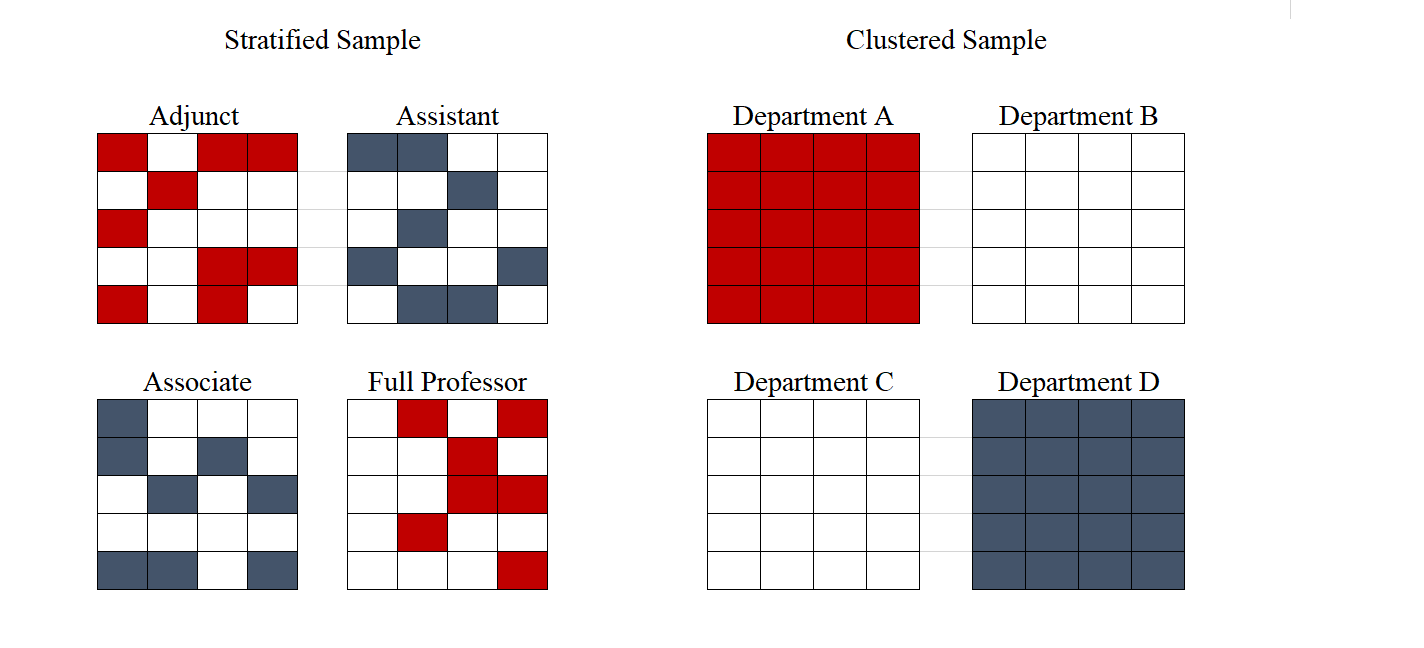
\includegraphics{images/data/samples.png}
\caption{Stratified vs.~Clustered sampling}\label{fig:samples}
}
\end{figure}

Not all surveys use probabilistic sampling, and you should be very wary of
these. One type of sampling method under this category is \textbf{convenience
sampling}. As its name suggest, this method implies selecting individuals that
are most accessible. Most online polls have this characteristic: the sample
will be composed of people who accessed certain websites where the poll was
posted and decided to take their time to answer it. A convenience sample could
also consist of surveying your soccer team when your research is about soccer
fans across the country. \textbf{Snowball sampling} is another type of
nonprobability sampling. This method is usually used when studying certain
vulnerable or hidden populations that are harder to reach through normal
sampling methods (eg. people with AIDS). With this technique, a survey
respondent will provide referrals who will be recruited to become part of the
study.

Nonprobability samples suffer from a major problem called \textbf{sampling
bias}. With these techniques, the resulting sample is far from reflecting the
actual population. The online poll example will be a representation only of
those people who are exposed to the poll and who feel compelled to answer it,
which has been shown to be nonrandom. Deciding to only survey your soccer team
will yield biased results as well. You will be representing only a certain age
group, from a certain neighborhood who probably share socio-economic status
and educational level. The results from this poll will not provide any
information on soccer fans across the country, but only of one limited,
unrepresentative portion of them.

Although the risks of falling into sampling bias is much lower with random
sampling, this might still occur. For instance, while it used to be common to
survey people through landline telephone surveys, this will nowadays exclude a
significant part of the population. For this reason, pollsters such as Pew
Research Center combine random sampling from both landline and cellphone
numbers. This method ensures that practically all of the U.S. population will
be covered (according to Pew, only 3\% of households have no phone
access).\footnote{https://www.pewresearch.org/methods/u-s-survey-research/our-survey-methodology-in-detail}

There are other types of biases that researchers must be aware of, both for
random and nonrandom samples. One of these is \textbf{non-response bias},
referring to subjects that do not wish to participate or answer certain
questions, or when subjects cannot be reached. The differences between those
that chose to respond and those that do not are usually nontrivial. For
instance, people who participate in a poll of a given subject tend to have
stronger feelings for it. If a pollster is calling people at 10am, people who
are at work will probably refuse to answer, and the differences between their
opinions and non-working people opinions are usually not random. This is why
pollsters attempt contact at different times of day and different days of the
week. Other types of biases can arise from question wording, social
desirability or respondent fatigue. You can learn about these in the chapter
on \emph{surveys}.

Finally, no matter how well designed your sampling method is, your results
will always have some \textbf{sampling error}. Sampling error accounts for the
fact that your results do not correspond to the population, but to your
sample. Inevitably, there exists variation between these two. The sampling
error is also called \textbf{margin of error}, and it depends on how many
subjects are in your sample and on how dispersed our data is. As mentioned
previously, the law of large numbers states that, the larger the sample, the
closer the estimate will be to the actual population value. Note, however,
that usually around 1,500 observations is large enough to represent a country.
In fact, most of the regional survey mentioned above, such as Afrobarometer
and Latinobarometer, survey between 1000 and 1200 subjects in each country.
Though the margin of error continues getting smaller as the size surpasses
1500, the gains are usually not worth the costs of surveying more people. On
the other end, the margin of error does vary substantially for lower sample
sizes.

Since we can never be 100\% confident that our result is exactly the same as
the population value, we must always calculate the margin of error to
represent the uncertainty of our estimates. Failing to consider this
uncertainty is one of the most common ways of misinterpreting survey results.
Going back to the example of your survey of university professors: imagine
your sample size is of 200 cases, with a margin of error of 8 percentage
points. Your estimates show that, among tenured professors, the average score
of student evaluations is of \(72\%\) , while for non-tenured professors it is
78\%. This could lead you to erroneously conclude that non-tenured professors
have higher student evaluations. In reality, given such high margin of error,
we cannot claim any difference between the scores. Our estimate of non-tenured
teacher evaluations are actually between \(71\%\) and \(86\%\)
(\(78\% \pm 8\)), while tenured professor evaluations are between \(64\%\) and
\(80\%\) (\(72\% \pm 8\)).

In sum, surveys are an essential tool in data collection, but must be designed
carefully in order to avoid common pitfalls. First, be aware of problems
related to sampling. When encountering surveys, always evaluate if the sample
on which the study was done is representative of the population for which
conclusions are being drawn. A study performed on a sample of students from
your cohort will only speak to the opinions of students from your university
and your cohort. Finally, yet very importantly, recall that survey estimates
will always have some variation from the actual "reality". You must take into
account this uncertainty and evaluate the results with their corresponding
margin of error.

\begin{shaded*}

\textbf{Check-in question:} The headline of a news article reads: "Candidate X
will win the elections by a large margin: poll shows 52\% of people support
her, while Candidate Y is only backed by 43\%." Why is this headline
misleading? What key piece of information is missing to correctly interpret
the difference in electoral support between the candidates?

\end{shaded*}

\hypertarget{measurement}{%
\section{Measurement}\label{measurement}}

Another aspect we must take into consideration before data collection is
specifically how our concept will be measured, or operationalized. Whichever
our data collection process is, we must be certain that what we are measuring
corresponds to the concept we wish to study. A good measurement must be
reliable and valid. \textbf{Reliability} means that every time you measure you
should obtain the same results. \textbf{Validity} refers to the fact that the
measure actually represents the concept we are interested in. As the figure
below illustrates, a measure can be reliable if all measures consistently
capture the same phenomenon, yet not valid if this phenomenon is not the same
as our concept. It can be neither reliable nor valid if it does not
consistently measure the same thing and that thing is not our concept. A
measure that is both reliable and valid will be correctly capturing our
concept in every iteration.

\begin{figure}
\hypertarget{fig:target}{%
\centering
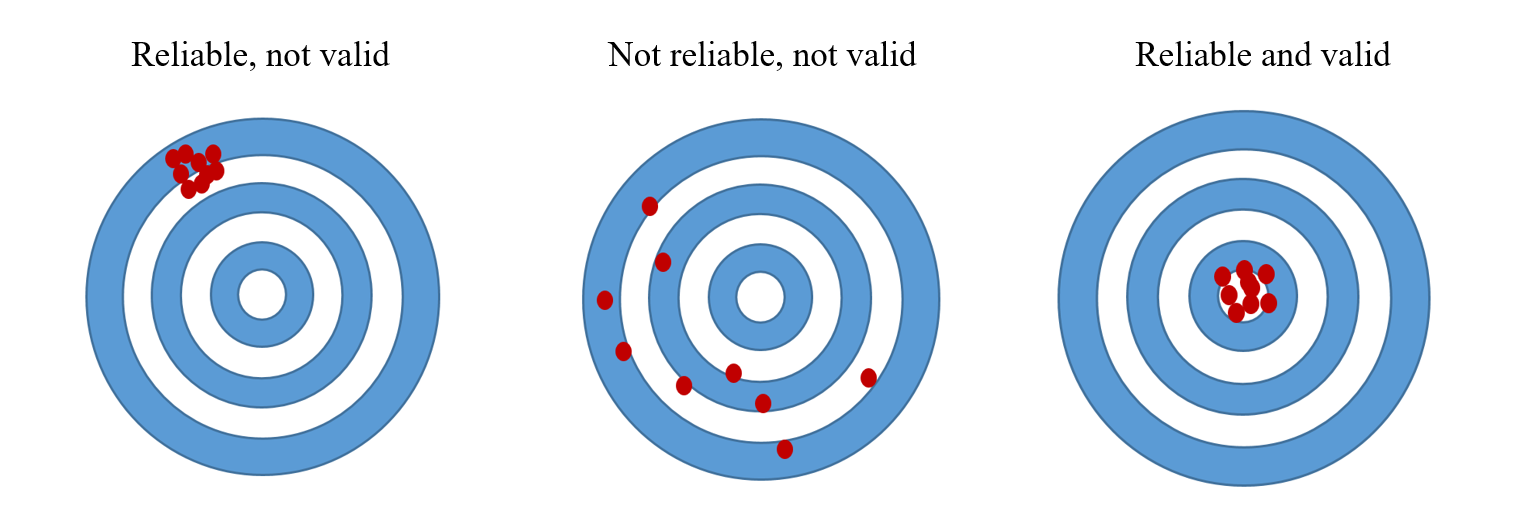
\includegraphics{images/data/target.png}
\caption{Validity and reliability}\label{fig:target}
}
\end{figure}

Problems of measurement are present beyond the use of surveys. Take the
concept of democracy, for which we can find at least 10 different measures.
The first differences among these measures is the way they are conceptualized,
or defined. This step requires researchers to establish which attributes will
be considered. Democracy measures usually include some combination of:
political rights, political participation, freedom of speech, civil liberties,
competitive elections, free and fair elections, etc. Then they vary according
to which indicators they chose for each attribute. What piece of information
do I consider to evaluate if a country has free elections? Will I code this as
a simple dichotomous variable (free/not free)? Or will it be a numerical
variable that captures the degree of freedom in elections? Lastly, since all
measures of democracy are in the form of an index, there must be an
aggregation rule. Are the scores of each attribute added or multiplied? Does
each indicator weight the same? All of these decisions will yield different
results. Table \protect\hyperlink{table:ux5cux2520data_democracy}{{[}table:
data\_democracy{]}} below, adapted from
(\protect\hyperlink{ref-munck2009}{Munck 2009}) illustrates how three
different measures of democracy are constructed. Note that the table omits two
further elements that distinguish the measures: the specific indicators chosen
for each component and the aggregation rules.

\begin{longtable}[]{@{}
  >{\raggedright\arraybackslash}p{(\columnwidth - 6\tabcolsep) * \real{0.3187}}
  >{\raggedright\arraybackslash}p{(\columnwidth - 6\tabcolsep) * \real{0.3077}}
  >{\raggedright\arraybackslash}p{(\columnwidth - 6\tabcolsep) * \real{0.1758}}
  >{\raggedright\arraybackslash}p{(\columnwidth - 6\tabcolsep) * \real{0.1758}}@{}}
\toprule
\begin{minipage}[b]{\linewidth}\raggedright
Name of index
\end{minipage} & \begin{minipage}[b]{\linewidth}\raggedright
Attributes
\end{minipage} & \begin{minipage}[b]{\linewidth}\raggedright
Components of attributes
\end{minipage} & \begin{minipage}[b]{\linewidth}\raggedright
Measurement level
\end{minipage} \\
\midrule
\endhead
3*(alvarez1996) & Contestation & & Nominal \\
(1)3-4 & 2* Offices & Election executive & Nominal \\
& & Election legislature & Nominal \\
6* (bollen1980) & 3* Political liberties & Press freedom & Interval \\
& & Freedom of group opposition & Interval \\
& & Government sanctions & Interval \\
& \textbackslash multirow\{3\}\{*\}\{Popular sovereignty\} & Fairness of
elections & Interval \\
& & Executive selection & Interval \\
& & Legislative selection and effectiveness & Interval \\
52.5cm Polity IV (marshall2001) & Competitiveness of participation & &
Ordinal \\
& Regulation of participation & & Ordinal \\
& Competitiveness of executive recruitment & & Ordinal \\
& Openness of executive recruitment & & Ordinal \\
& Constraints on executive & & Ordinal \\
\bottomrule
\end{longtable}

\textbf{Table 4.1: Conceptualization and measurement of democracy, according
to different authors, source: Adapted from (Munck 2009)}

One concrete example of how a "small" change in measurement can substantially
change a measure of democracy comes from Paxton
(\protect\hyperlink{ref-paxton2000}{Paxton 2000}), who analyzes scholarly
literature that indicates when a country democratized. She scrutinizes
authors' definitions of democracy, which in most cases consider a country to
become democratic when suffrage is universalized. However, these definitions
are not always consistent with the dates coded as transitions, since female
suffrage is introduced much later. Switzerland is one of the most clear cases:
women were allowed to vote only in 1971, yet all of the authors contemplated
in Paxton's study consider it to have been a democracy since the 19th century.

No matter how careful we are in the operationalization of our concept, there
will always be some error in our measurement. Yet, not all errors will have
the same effect on our results. Systematic errors, or systematic bias, are the
most damaging. \textbf{Systematic bias} occurs when we are consistently making
a mistake in our measurement. In a scientific lab experiment, for instance,
our experiment will have systematic bias if our measuring tool is not
calibrated correctly, and so every single measure will be off to some extent.
When conducting surveys, systematic bias results from errors in sampling
(sampling bias), but also from factors such as question wording and order.
This bias also occurs with other data collection methods. Following Paxton, if
an author identifies a transition to democracy when suffrage is truly
universalized, yet considers countries where women did not have the right to
vote as democracies, then this is a case of systematic bias.

While systematic bias generally follows a pattern, \textbf{random measurement
error} is due to chance. As opposed to systematic bias, random error does not
have a distinct upward or downward bias, and thus it does not have a
significant impact on our results. In other words, we might be off in our
measurement, but our errors are randomly distributed throughout our data; they
do not have a distinct upward of downward direction. Essentially, all or the
errors should balance each other out and average out to zero. When we use
Likert scales in surveys (e.g.~"In a scale of 1 to 10, where 1 is strongly
disagree and 10 is strongly agree..."), some might respond too high and others
too low, but, on average, we will capture the spirit behind it. When we have
an \textbf{unreliable measurement}, however, our amount of random error has
become too large. What exactly is too much error is not clear, however.

\begin{shaded*}

\textbf{Check-in question:} A researcher wants to obtain a measure of average
wages in a country. To do so, she collects data from the social security
agency, which centralizes information from each company's payroll. Yet, this
country has a large informal economy, meaning many workers are paid "under the
table", and thus will be left out of her measure. What type of error does this
represent?

\end{shaded*}

\hypertarget{measures-of-central-tendency}{%
\section{Measures of Central Tendency}\label{measures-of-central-tendency}}

Once we have collected our data, our first step is to become familiarized with
it before doing any complex statistics. We need to get a picture of what the
data looks like. A first way of summarizing data is through tables and graphs,
such as frequency tables, histograms, bar graphs, etc. Effectively
illustrating data is an enormous advantage. In this section, though, we will
focus not on tables and graphs but on statistical measures that summarize
data. The first family of statistics, the measures of central tendency, are
useful to describe the center of the data, what a typical observation is like.
There are three measures of central tendency: the mean, the median, and the
mode.

The \textbf{mean}, also known as the average, is calculated by adding up all
the values of that variable and dividing by the amount of observations. It is
the most widely used summary statistic since it a balancing point in the
distribution and gives a sense of where most values fall near. Of course,
given that it involves a mathematical operation, it is only applicable to
numeric variables, as opposed to nominal and ordinal ones. One disadvantage of
the mean is that it is sensible to outliers. Outliers, or values that are
substantially higher or lower than the rest, can pull the mean in that
direction, thus resulting in a misleading representation of the typical
observation. This is especially true as the sample gets smaller; the smaller
the sample, the more each observation weighs. For example, lets consider the
average income of the people in a small seminar. The ten attendees are
students, whose monthly incomes range from \(\$1,000\) to \(\$2,600\). Yet,
the speaker in the room is a famous businessman who earns \(\$60,000\) a
month. The average income of the room is \(\$7,054\), yet all ten students
earn less than \(\$3,000\). In this case, the mean is not the most appropriate
measure of the "typical" observation.

A second measure of central tendency, the \textbf{median}, could be a better
fit for the above example. The median is the number that marks the center of
the distribution when the values are listed in numerical order. It divides the
distribution in exactly half. When the number of values is even, the two
numbers at the center are averaged. To calculate the median from the above
example, we first order the incomes from lowest to highest: \$1,000, \$1,000,
\$1,000, \$1,100, \$1,200, \$2,300, \$2,400, \$2,500, \$2,500, \$2,600,
\$60,000. Then we identify the midpoint in the distribution: \$2,300. This is
a far better representation of the room's average income. Thus, when a certain
variable has outliers, the median is usually the preferred method to describe
the center. Another advantage it has over the mean is that it can also be used
to describe ordinal (but not nominal) data. However,in cases with few response
categories, the median can give little information about a distribution. Two
sets of numbers could have the same median yet different patterns.

The last measure of central tendency is the \textbf{mode}. The mode is the
value that is occurs most often. This measure can be used with any type of
variable, yet it is especially useful for categorical data. However, if the
most common value is not a significant portion of the distribution, the mode
might be trivial. Note that a distribution may have more than one value with
an exceptionally high occurrence. In our example, the mode was 1,000. Bi-modal
distributions are such cases, where the distribution will have two peaks at
distinct values. Distributions can also be multimodal, or uniform in cases
where all the values have the same frequency.

All three measures are complementary when describing the center of data.
Furthermore, having these three measures provides a sense of how the data is
shaped. If the mean, median and mode are similar, the distribution is
symmetrical. When the mean is below the median and the mode, it means there
are extreme values in the lower half of the distribution that are pulling the
mean towards that end. This results in a \textbf{negatively skewed
distribution}. On the contrary, high extreme values pull the mean towards the
upper end, thus resulting in a \textbf{positively skewed distribution}. In
addition, based on the number of modes, we have information on the modality of
the distribution.

\begin{figure}
\hypertarget{fig:plots}{%
\centering
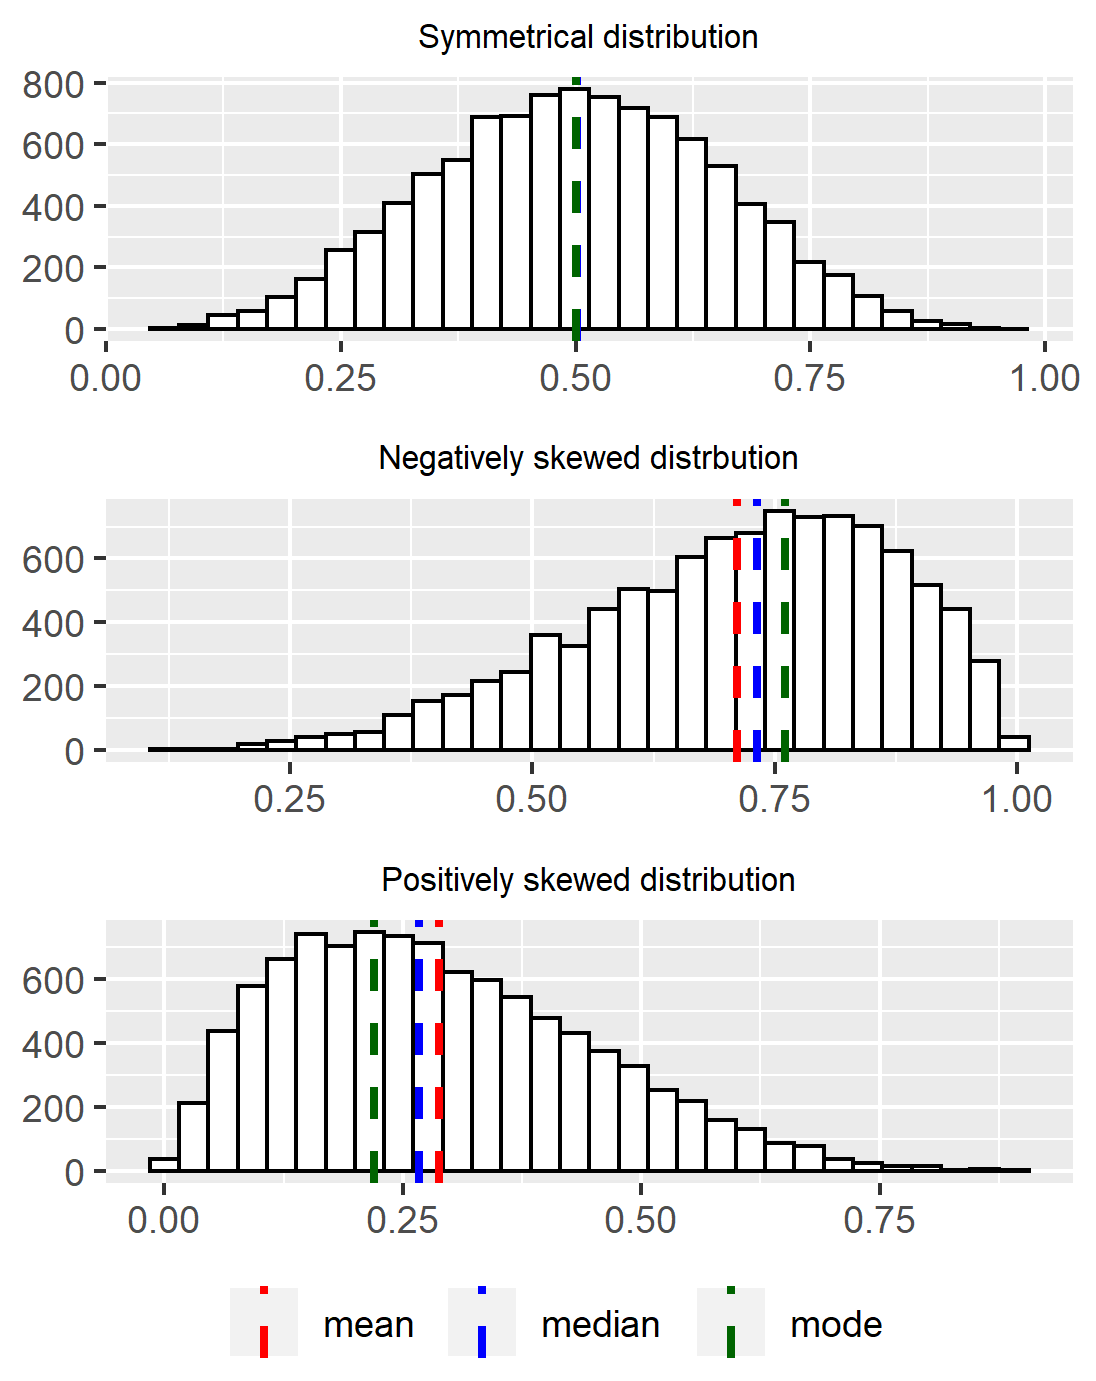
\includegraphics{images/data/plots.png}
\caption{Types of distributions}\label{fig:plots}
}
\end{figure}

Whereas the measures of central tendency give us insight into the center of
the data and the typical values, measures of dispersion characterize how
spread out the data is. One of such measures is the \textbf{range}. A range
measures how far apart the highest and lowest value are. If votes for Party A
are as low as 10\% in one region and as high as 90\% in another, the range is
of 80\%. If Party B obtains 25\% in the least supportive region and 60\% in
the most supportive, its range is of 35\%. Party B has less variability.

Two other measures of dispersion widely used in statistic are the
\textbf{variance} and the \textbf{standard deviation}. The standard deviation,
which is a slight transformation of the variance, is more widely used because
it is easier to interpret. Simply put, they measure the average distance of
each observation from the mean. Larger standard deviations indicate more
dispersion in the data. Note that standard deviation must always be positive:
there is no such thing as a negative distance. The calculation of the variance
and standard deviation is straightforward, yet requires a few steps:

\begin{itemize}
\item
  Calculate the mean
\item
  Subtract each observation from the mean, and square the result
  (\((x_i -\bar{x})^2\))
\item
  Add up all squared deviations (\(\sum_{i=1}^{N}(x_i -\bar{x})^2\))
\item
  Divide by the number of observations (n) when dealing with a population or
  by the number of observations minus 1 (n-1) when dealing with a sample. Up
  to this point, you have calculated the average distance from each
  observation to the mean, squared. This is what we call the variance
  (\(\frac{\sum_{i=1}^{N}(x_i -\bar{x})^2}{(n-1)}\)). For a more intuitive
  interpretation, though, we add one more step:
\item
  Take the square root of the variance to obtain the standard deviation
  (\(\sqrt{\frac{\sum_{i=1}^{N}(x_i -\bar{x})^2}{(n-1)}}\))
\end{itemize}

In sum, an essential description of any variable should include these basic
measures to describe both its typical values and to describe their variation.

\hypertarget{broader-significanceuse-in-political-science}{%
\section{Broader significance/use in political
science}\label{broader-significanceuse-in-political-science}}

The issues discussed in this chapter are encountered in every single research
process. In Political Science, and social sciences in general,
conceptualization and measurement are particularly contested issues. Given the
nature of the discipline, most, if not all of our approaches to research have
some degree of subjectivity. This does not mean, however, that they fail to be
scientific. But in order to make legitimate and persuasive arguments, we need
to make extra efforts to create robust measures of our concepts. These topics
are so relevant that an important part of methodological training is focused
specifically on them (\protect\hyperlink{ref-goertz2006}{Goertz 2006};
\protect\hyperlink{ref-sartori1970}{Sartori 1970};
\protect\hyperlink{ref-collier2009}{Collier and Gerring 2009}).

Sampling is also very tightly linked to the Political Science discipline.
Particularly when studying individuals, you will frequently encounter research
questions that refer to a broad population which is impossible to completely
collect data from. This is why good samples are fundamental to the process.
Valid and reliable results hinge upon well designed samples.

\hypertarget{conclusion-2}{%
\section{Conclusion}\label{conclusion-2}}

Data is (are)\footnote{Some prefer data as plural while others refer to data
  as singular. Either way is fine!} the building blocks of research. Without
it, we cannot do science. Yet not all data is equally valuable, and no data is
ever objective. Whichever the source of our data is we must be very well
acquainted with it and be aware that every one of its characteristic will have
different impacts on our results. Keep in mind all the types of bias data may
have. Starting with concept formation, be wary that no concept is the same,
and make transparent and thoughtful decisions as to why you chose to build and
measure the concept the way you do. Also, pay close attention to how the data
is being collected. Recognize that none of these choices are neutral, that
they all have limitations, and that they will have different consequences on
your research. Once you have your data collected, dedicate time to describing
your dataset. This will reveal interesting trends and patterns that are
valuable in and of themselves, as well as provide you with a useful guide for
more advanced statistical analysis.

\hypertarget{application-questions-2}{%
\section{Application Questions}\label{application-questions-2}}

\begin{enumerate}
\def\labelenumi{\arabic{enumi}.}
\item
  Consider the distribution of poverty rates in Latin America. Calculate the
  measures of central tendency. Which do you think best summarizes the data?
  What happens if you exclude Haiti from your calculations? What happens if
  you exclude Uruguay from your calculations?

  \begin{longtable}[]{@{}lc@{}}
  \caption{Poverty headcount ratio at \(\$3.20\) a day (2011 PPP), \% of
  population.}\tabularnewline
  \toprule
  Country & Poverty rate \\
  \midrule
  \endfirsthead
  \toprule
  Country & Poverty rate \\
  \midrule
  \endhead
  Argentina & 2 \\
  Bolivia & 11.8 \\
  Brazil & 9.6 \\
  Chile & 1.8 \\
  Colombia & 10.8 \\
  Costa Rica & 2.7 \\
  Dom. Rep. & 5.9 \\
  Ecuador & 8.7 \\
  El Salvador & 8.5 \\
  Guatemala & 24.2 \\
  Haiti & 50.8 \\
  Honduras & 31.6 \\
  Mexico & 11.2 \\
  Nicaragua & 12.8 \\
  Panama & 6.3 \\
  Paraguay & 5.6 \\
  Peru & 9.8 \\
  Uruguay & 0.4 \\
  \bottomrule
  \end{longtable}
\item
  A researcher wants to study ethnic diversity in the city of Chicago. Explain
  why each of these sampling strategies could work (or not) for this purpose:

  \begin{enumerate}
  \def\labelenumii{\arabic{enumii}.}
  \item
    Interviewing the first 200 people they see at their neighborhood Whole
    Foods.
  \item
    Randomly sampling 2 neighborhoods in Chicago and interviewing all their
    residents.
  \item
    Randomly sampling 100 people in each neighborhood of Chicago.
  \end{enumerate}
\item
  Consider Paxton's study referenced above. Are the measures of democracy that
  Paxton criticizes valid, reliable, both, or neither?
\end{enumerate}

\hypertarget{key-terms-1}{%
\section{Key Terms}\label{key-terms-1}}

\begin{itemize}
\item
  aggregation
\item
  bias
\item
  cluster sampling
\item
  conceptualization
\item
  continuous
\item
  convenience sample
\item
  coverage bias
\item
  cross-sectional
\item
  dichotomous (dummy) variables
\item
  disaggregation
\item
  level of analysis
\item
  longitudinal data
\item
  margin of error
\item
  mean
\item
  median
\item
  mode
\item
  nominal
\item
  ordinal
\item
  panel data
\item
  population
\item
  sample
\item
  sampling error
\item
  sampling frame
\item
  skewness
\item
  standard deviation
\item
  systematic measurement error
\item
  time series data
\item
  unit of analysis
\end{itemize}

\hypertarget{answers-to-application-questions-2}{%
\section{Answers to Application
Questions}\label{answers-to-application-questions-2}}

\begin{enumerate}
\def\labelenumi{\arabic{enumi}.}
\item
  How could age be operationalized as different type of variables? Age could
  be a discrete variable if asked in whole years or it could be an ordinal
  variable if asked in intervals (eg. Under 18 years old, Between 18 and 50
  years old; Above 50).
\item
  Description of Uruguayan Survey. What type of data is this? A panel data.
  What is the population being studied? Children that attended first grade at
  public primary schools in Montevideo and urban areas in 2004.
\item
  Why is this headline misleading? What key piece of information is missing to
  correctly interpret the differences in electoral support between the
  candidates? In order to accurately describe the difference among candidates
  we need to know what the margin of error is. If the margin of error is of
  9\%, for example, the support of each candidate would not be different.
  Support for Candidate X would be between \(43\%\) and \(61\%\) and support
  for Candidate Y would be between \(34\%\) and \(52\%\).
\item
  If a researcher wants to measure average wages in a country with a large
  informal economy, yet she is only considering data from the formal economy,
  her measurement will have a systematic error because she is leaving out a
  large portion of workers. Her measure of average wages will probably be
  inflated, since informal workers tend to get paid less than formal workers.
\item
  \begin{enumerate}
  \def\labelenumii{\arabic{enumii}.}
  \item
    Mean: \(11.9\), Median: \(9.15\), Mode: - , Range: \(50.4\), Standard
    Deviation: \(12.04\)
  \item
    By excluding Haiti, the mean lowers to \(9.6\), the median \(8.7\), the
    range to \(31.2\) and the standard deviation to \(7.7\).
  \item
    By excluding Uruguay, the mean increases to \(12.6\), the median to
    \(9.6\), the range to \(49\), and the standard deviation to \(12.05\).
  \item
    The case of Haiti is particularly disruptive to the mean. When it is
    included in the calculations, the median is a better representation of the
    typical poverty levels of the region.
  \end{enumerate}
\item
  \begin{enumerate}
  \def\labelenumii{\arabic{enumii}.}
  \item
    Interviewing the first 200 people in the neighborhood Whole Foods is an
    example of a convenience sampling. This will surely bias the results for
    the study since there is low probability that the interviewees represent
    the ethnic heterogeneity of Chicago's residents.
  \item
    Randomly sampling 2 neighborhoods in Chicago and interviewing all their
    residents could work better than the first alternative, but it still has
    problems. Given that Chicago is such a segregated city, we run the risk of
    sampling two very homogeneous neighborhoods. Maybe we sample one
    neighborhood with mostly White residents and one with mostly Hispanic
    residents, in which case we would not be considering all other races and
    ethnic backgrounds.
  \item
    Randomly sampling 100 people in each neighborhood of Chicago would be the
    best option. It would be the most costly, but the sample would probably
    include people from many ethnic backgrounds.
  \end{enumerate}
\item
  If an author considers that a country's transition to a democracy occurred
  when they had universal suffrage, yet they code cases as transitions where
  only male suffrage was universalized, then this is an example of a reliable,
  yet not valid measurement. It is reliable if every single case is measured
  the same way, but not valid because the concept they are measuring does not
  correspond to their definition of democracy.
\end{enumerate}

\hypertarget{hypothesis-testing}{%
\chapter{Hypothesis Testing}\label{hypothesis-testing}}

\textbf{By Zhihang Ruan}

\hypertarget{introduction-4}{%
\section{Introduction}\label{introduction-4}}

Either in our daily lives or in scientific research, we come across a lot of
claims. We may formulate our own hypotheses based on our knowledge, available
information, or existing theory. These hypotheses can be descriptive, e.g., we
may hypothesize that a certain percent of U.S. voters support the policy of
universal basic income. Or the hypothesis can be causal, e.g., we may believe
that education leads to stronger support for gender equality. The measures
(for example, mean or standard deviation) used to describe a population
distribution are called \textbf{population parameter}. If we have access to
everyone among the population we are interested in, then we may easily tell
whether our hypothesis of a population parameter is true or false (e.g., if we
know every voter's support for the policy of universal basic income, then we
can prove/disprove our hypothesis concerning the support rate for the policy).
But in many cases, we do not have access to the population to firmly prove or
disprove our hypotheses. For example, it may cost too much to ask each U.S.
voter about their opinions on specific policies. In these cases, statistical
theory and methods provide us some effective ways to test a hypothesis, or
more accurately, assess whether the observed data is or is not consistent with
a claim of interest concerning the population. In this chapter, we will go
through the idea of hypothesis testing in statistics and how it is applied in
political science.

\hypertarget{background}{%
\section{Background}\label{background}}

There are different understandings of hypothesis testing. In this chapter, we
will follow the Neyman-Pearson paradigm
(\protect\hyperlink{ref-rice2007math}{Rice 2007, 331}), which casts hypothesis
testing as a decision problem. Within this paradigm, we first have a null
hypothesis and an alternative hypothesis concerning the population. A null
hypothesis is a claim or hypothesis we plan to test, or more specifically,
something we decide whether to reject or not. It can be descriptive (e.g., the
support rate for the president among all U.S. voters) or causal (education
leads to stronger support for gender equality among all human beings). An
alternative hypothesis is also called the research hypothesis, which is
opposite to the null hypothesis. It is what we believe to be true if we reject
the null hypothesis. Then with what we observe in a random sample from the
population, we make a decision to reject or not reject the null hypothesis
concerning the population. This approach does not enable us to say the exact
probability that the null or alternative hypothesis is true.\footnote{This may
  be a bit confusing. But you may consider it this way. Let's say, we
  hypothesize that the average height of all Northwestern undergrads is 5.7
  feet. If we do the hypothesis testing as we will learn in this chapter, we
  will not reject the null hypothesis unless we get a random sample whose
  average height is much higher than 5.7 or much lower than 5.7 feet. In many
  cases, we may not reject the hypothesis. However, how likely is the
  hypothesis true, even if we do not reject it? Almost 0, because the exact
  average height can be any number slightly different from 5.7 feet, e.g.,
  5.700001 or 5.697382. As a result, the hypothesis is almost always wrong,
  but we do not always reject it. Thus, whether to reject the hypothesis or
  not does not tell us whether it is true or false. Nor does it tell us the
  probability that it is true.} To do that, we need more information and maybe
another paradigm (e.g., so-called prior probability within the Bayesian
paradigm), and we will not go in details in this chapter. But, even though the
approach we discuss in this chapter does not directly tell us how likely a
hypothesis is true or false, the approach is very useful in scientific studies
as well as daily lives, as you will see in this chapter.

As mentioned in the introduction of this chapter, the classic idea of
hypothesis testing concerns a sample and a population. In the previous
chapter, we learned what the terms population, random sample and random
sampling mean. The techniques we discuss in this chapter mostly assume a
random sample. Below, we will quickly review the idea of random sampling and
random sample and explains how random sampling enables us to make inference
about the population with what we observe in the sample.

\hypertarget{samples-and-sampling-1}{%
\section{Samples and Sampling}\label{samples-and-sampling-1}}

As mentioned in the beginning of this chapter, in many cases, we do not have
the access to all the units of the population we are interested in. For
example, if we are interested in the support rate for the president, it would
be perfect if we know the opinion of every single person (i.e., unit of the
population) in the U.S. However, it is almost impossible to get access to
everyone's opinion. In many cases, we can only get access to a small group of
individuals, which we call a sample from the population. When the sample is
randomly chosen from the population (i.e., everyone in the population has an
equal chance to be selected, or at least has a specific chance known to the
researchers before the sample is drawn), then we may learn about the
population with what we observe in the random sample we have. More
specifically, statistical theory enables us to make inference about the
population from the random sample. In the next part, I will explain how we may
make inference from a random sample to the population and test a hypothesis
concerning the population with a random sample.

\hypertarget{magic-of-the-central-limit-theorem}{%
\subsection{Magic of the Central Limit
Theorem}\label{magic-of-the-central-limit-theorem}}

Let's say, we roll a fair die. We know the probability of getting 1 is 1/6. In
other words, the probability that the mean of the number we get from one trial
equals 1 is 1/6. Then, if we roll the same die twice, we get two numbers. We
can calculate the mean of the two numbers. What is the probability that the
mean equals 1? Is the probability still 1/6? No, because if the mean is 1, we
have to get 1 twice, the probability of which would be 1/36 (which equals 1/6
times 1/6). Very likely, the mean we get is larger than 1. Similarly, if we
roll the die three times, the mean of the three numbers we get would probably
be larger than 1. If we roll the die many times (e.g.~1,000 times), it is
almost impossible that the mean would be 1 or even close to 1 (since it means
we need to get 1 in all or most of the trials). Then what would the mean be?
The mean would not be an extreme number like 1 or 6. Instead, it would be very
close to the expected value we get from rolling it once, which is 3.5, the
average of all possible numbers we get. Among the 1,000 trials, the number of
1s we get would be close to the amount of 2s we get, or the amount of 3s, etc.
If we take the average of all numbers we get in the 1,000 trials, we would get
a number very close to 3.5, which equals (1+2+3+4+5+6)/6.

This is what we call the weak law of large numbers: the sample average
converges in probability towards the expected value or the population average,
or in other words, the average of the sample gets close to the population
average when the sample size is large (e.g., when rolling the die 1000 times).

One step further from the law of large numbers, we can rely on something
called the central limit theorem to make inference. The \textbf{central limit
theorem} suggests that the mean of a sufficiently large number of independent
draws from any distribution will be normally distributed. A normal
distribution is a bell-shaped probability density. From the example above, we
already know the mean of a large amount of draws is very close to the expected
value of the population. But in most cases, the average of the draws will not
be exactly equal to the expected value of the population (which is 3.5 in the
example of rolling a fair die). The central limit theorem enables us to
calculate/quantify the probability that the sample average falls into
intervals around the expected value of the population. As long as the expected
value and variance of a normal distribution is known, we can calculate the
probability that we get a sample mean within a specified interval. For
example, with some calculation based on the central limit theorem (which we
will not go into details here), we know that if we roll a fair die 1,000
times, the chance that the mean of the 1,000 numbers we get falls between
3.394 and 3.606 is roughly 0.95 (or 95 percent).

What if, after rolling the die 1,000 times, the average of the 1,000 numbers
we get is much smaller than 3.394 or much larger than 3.606? Then we may want
to check whether there is some problem with the rolling process, or whether
the die is fair. Similarly, if we hypothesize that the support rate for the
president is 50 percent, but after interviewing 1,000 people randomly drawn
from the population, we find that the support rate is much lower than 50
percent, then we may doubt whether the support rate is really 50 percent. This
makes sense when the sample is drawn randomly from the population. But if the
sample is not drawn randomly (e.g., all the people in the sample are drawn
from a gathering of a specific party), then the result does not tell us much
about the support rate among the population. This is like a magician who uses
tricks and gets 1 every time rolling a fair die. We cannot learn anything
about the die based on the mean the magician gets.

These examples show us how central limit theorem works and how it makes
hypothesis testing possible. In the next part, I will explain more
specifically how we may estimate the population average/expected value based
on what we observe from the sample, as well as how to test a hypothesis.

\hypertarget{estimates-and-certainty}{%
\section{Estimates and Certainty}\label{estimates-and-certainty}}

Based on the central limit theorem, we can make inferences about the
population with the data we observe. One way to estimate the population
parameter is called \textbf{point estimate}, which is a sample statistic used
to estimate the exact value of a population parameter. We may consider the
point estimate as our best guess to the population parameter based on what we
observe in the sample. For example, if we learn that the mean of a random
sample from simple random sampling is 3.5, then we may say that the point
estimate of the population mean is 3.5.

But in most cases, the point estimate does not equal the true value of the
population parameter (e.g., the population mean can be 3.5001, 3.4986 or other
number when the sample mean is 3.5). Another way to estimate the population
parameter is interval estimation. With the information we learn from the
sample, we may calculate an interval that may include the population average.
The central limit theorem enables us to quantify how confident we are that the
interval will include the population average. The interval is called
\textbf{confidence interval}, which defines a range of values within which the
population parameter is estimated to fall. If we want to estimate the
confidence interval of the population mean, we need the sample mean, the
estimated population variance, and the sample size. A 95 percent confidence
interval for the population mean equals \(\bar{X}\pm 1.96 * (S_{\bar{X}})\).
\(S_{\bar{X}}\) is the estimated standard error of the sampling distribution
of the sample mean. It is equal to the standard error (or the square root of
the variance) of the population divided by the square root of the sample
size.\footnote{We have 1.96 in the formula because statisticians tell us if we
  randomly draw a number from a normal distribution, we have a 95 percent
  chance of getting a number no more than 1.96 standard errors above or below
  the mean of the distribution.} We can see from the formula that the range of
the interval will decrease when the population variance is small, and the
sample size is large. This makes sense intuitively because when there is
little variation among the population, or when we have a large sample, the
sample mean may be close to the population mean, and thus our estimation will
be more precise.

In short, we can estimate the confidence interval of the population mean based
on the sample we get. Similarly, if we have a hypothesis about the population
average, then we can calculate an interval which the sample mean may fall
into, and quantify how confident we are that the sample average will fall onto
this interval.

It is intuitive to say that if we increase the range of our estimated
interval, we are more confident that the interval will include the population
mean. The trade-off is that our estimation is less precise. The likelihood,
expressed as a percentage or a probability, that a specified interval will
contain the population parameter, is called \textbf{confidence level}. For
example, if we learn from a random sample (with a sample size of 1,000) that
the support rate for the president is 52 percent, then a 95 percent confidence
interval of the support rate among the population is between 50.5 and 53.5.
And a 99 percent confidence interval is roughly 50.0 to 54.0 percent. As we
can see, the confidence interval becomes wider (in other words, our estimation
becomes less precise) if we want to be more confident that the population mean
is within the confidence interval we estimate (i.e., we have a higher
confidence level). More specifically, a 99 percent confidence interval for the
population mean equals \(\bar{X}\pm 2.58 * (S_{\bar{X}})\).\footnote{We have
  2.58 in the formula because if we randomly draw a number from a normal
  distribution, we have a 99 percent chance of getting a number no more than
  2.58 standard errors above or below the mean of the distribution.} As we can
see, the interval is wider than the 95 percent confidence interval, which is
\(\bar{X}\pm 1.96 * (S_{\bar{X}})\), and the 90 percent confidence interval,
which is \(\bar{X}\pm 1.64 * (S_{\bar{X}})\).

\hypertarget{steps-of-hypothesis-testing}{%
\section{Steps of Hypothesis Testing}\label{steps-of-hypothesis-testing}}

Hypothesis testing becomes more straightforward once we understand the central
limit theorem and confidence interval. As mentioned earlier, if we have a
hypothesis of the population mean, then we can calculate a confidence interval
that the sample average will fall into. But if the sample average is very
different from the population average we hypothesize, or in other words, falls
outside the confidence interval at a specific confidence level, then we may
reject the null hypothesis with a specific level of confidence. For example,
if we hypothesize a die is a fair one, then the expected value (or the
population mean) we get from rolling the die once is 3.5. However, if we roll
the die many times (e.g., 1000 times), and the mean of all the numbers we get
is 2.003, then we may be very confident to say that the die is not a fair die
(i.e., we will reject the null hypothesis that the die is a fair one).

More specifically, there are four steps of hypothesis testing. First, we need
to have a statement about a population parameter evaluated with a test
statistic. The parameter can be the population mean (e.g., the average number
of basketball games Americans go to), proportion (e.g., the support rate for
the president among all U.S. voters), or some other characteristics of the
population, like the variance of heights among all first-grade children. Any
statement concerning the population implies a null hypothesis and an
alternative/research hypothesis concerning the population. The
\textbf{research hypothesis} is the hypothesis we're putting forward to test,
which reflects the substantive hypothesis. It is also called `alternative
hypothesis', but some prefer `research' to convey that this hypothesis comes
from an understanding of the subject area and is often derived from theory.
The research/alternative hypothesis is in contrast to the \textbf{null
hypothesis}, which is the `default' one that we wish to challenge. For
example, if most people believe that on average individuals in the U.S. go to
more than 1 basketball game annually, and we hypothesize that on average
Americans go to fewer than 1 basketball game every year. Then we can set our
hypothesis as the research hypothesis and the common belief as the null
hypothesis.

Then, we collect a random sample, calculate the statistic from the sample, and
compare the statistic with the null hypothesis and the alternative hypothesis.
What kind of statistic is calculated depends on the kind of hypothesis we have
and statistical methods we use in hypothesis testing. For example, if we are
interested in the population mean, then we need to calculate the mean and
standard error of the sample.

Then we determine the rejection of the null hypothesis or of failure to reject
the null. If the statistic we observe differs significantly from what we
hypothesize, then we will reject the null hypothesis. Otherwise, we fail to
reject the null hypothesis. As stated earlier, in most cases what we get from
the sample is different from what we state in the null hypothesis. But we
reject the null hypothesis only when what we observe in the sample is really
weird or significantly different from the null hypothesis. What counts as
weird, depends on the rule we set before, as well as common practices in the
field. In social science, we usually take a pretty strict standard concerning
the rejection of the null hypothesis. In many cases, only when the sample mean
is outside the 95 percent, 99 percent or 99.9 percent of the confidence
interval, do we reject the null hypothesis. This means, that we would expect
to get a result as `weird' as ours less than 5\% of the time, if the null
hypothesis is true. Since the probability is so low (e.g., 0.05), we reject
the null hypothesis.

We tend to be conservative and decide not to reject the null hypothesis. Thus,
failing to reject the null hypothesis does not mean the hypothesis is true,
but just means that we do not have enough evidence to reject it. Similarly,
rejecting the null hypothesis does not mean we prove that it is false, but it
only suggest that we have pretty strong evidence (that we feel confident
about) that it is false, if all the assumptions of the sampling process and
statistical methods we use are met (e.g., the sample is a random sample from
the population).

\hypertarget{types-of-hypothesis-testing}{%
\section{Types of Hypothesis testing}\label{types-of-hypothesis-testing}}

In our lives, we may have different types of claims or hypotheses. It can be a
hypothesis about the mean of the population (e.g., the support rate for the
president, the average income, etc.) or the variance of the population (e.g.,
the variance of people's income). Or it can be a hypothesis concerning the
difference between two groups, or a hypothesis about the correlation between
two variables. Statisticians have developed different tests for different
types of hypotheses. In this section, we will introduce some basic methods of
hypothesis testing.

\hypertarget{single-mean-hypothesis-testing}{%
\subsection{Single Mean Hypothesis
Testing}\label{single-mean-hypothesis-testing}}

The single mean hypothesis testing concerns the mean of the population we care
about. In many cases, we are interested in the population average. For
example, in an election, we may want to know the support rate for a specific
candidate, which is important for the development of campaign strategy. We may
hypothesize that the support rate for the candidate is a specific number, and
we can test the hypothesis with a random sample we get from the population. If
the support rate for the candidate among the sample is very different from the
rate stated in our hypothesis, we may reject the hypothesis. If the rate we
get from the sample is not very different from the number stated in the
hypothesis, we may fail to reject the hypothesis.

Here is how a single mean hypothesis works. As we have discussed, the central
limit theorem suggests that the mean of a random sample with a sufficiently
large sample size is normally distributed. The normal distribution of the
sample mean is an example of \textbf{sampling distribution}, which is a
theoretical distribution of all possible sample values for the statistic which
we are interested. For example, when we have a sample (with the sample size of
1,000), we can calculate the sample mean. If we do the sampling multiple times
(e.g., 1 million times), we get 1 million samples and 1 million sample means
(each sample still has 1000 cases). From the central limit theorem, we know
that the 1 million sample means follow a normal distribution. This
distribution is the sampling distribution of the sample mean, for samples with
the sample size of 1,000.

If we get a simple random sample (explained in the previous chapter), the
expected value of the sampling distribution of the mean equals the population
mean, and the variance of the sampling distribution is determined by the
population variance and the size of the sample. When there is less variation
among the population, or we have a larger sample, the variance of the sampling
distribution is smaller, which means the sample mean is expected to be closer
to the population mean.

Since the sampling distribution of the mean is a normal distribution, we can
calculate the probability that the sample mean falls into a specific range
given the hypothesis is true. If the sample mean we get is very different from
the hypothesized population mean, we may think there is some problem with the
null hypothesis and we may reject the null hypothesis. Statisticians have
learned a lot about the normal distribution, and we know that if we randomly
draw a number from a normal distribution, we have roughly 95 percent chance of
getting a number within two (or more accurately, 1.96) standard deviations
(which equals the square root of the variance) away from the expected value of
the normal distribution. Since the sampling distribution of the sample mean is
a normal distribution, the chance that the distance between the sample mean we
observe and the expected value of the normal distribution is more than two
standard deviations of the normal distribution is roughly 5 percent. Thus, if
we observe a difference between the sample mean and the hypothesized
population mean that is larger than twice the standard deviations of the
sampling distribution, we may reject the null hypothesis at the significance
level of 95 percent. It is weird (e.g., less than 5 percent chance) to get a
sample mean as extreme as the one we have if the null hypothesis is true, so
we decide to reject the null hypothesis. We can also set a stricter standard
(e.g., a significance level of 99 percent, or 99.9 percent) and reject the
null only when the difference between the sample mean and the population mean
is more extreme.

\hypertarget{difference-of-means-hypothesis-testing}{%
\subsection{Difference of Means Hypothesis
Testing}\label{difference-of-means-hypothesis-testing}}

Sometimes, we are not interested in the mean of a single group, but more
interested in the difference of means between two groups. Testing the
difference of means is especially useful when we aim to make causal inference
with an experiment. It can also be useful when we compare two groups without
aiming to make causal inference. For example, in an election, especially an
election within the majority system, we may be interested in whether one
candidate has a higher support rate than another candidate. In this case, we
are dealing with a hypothesis concerning the difference of means. The
hypothesis may take the forms of \(A>B\), \(A<B\), \(A=B\), or \(A-B=c\). If
our research hypothesis is \(A>B\), the null hypothesis would be \(A<B\). Then
we test the hypothesis with what we observe in the random sample. For example,
if the null hypothesis is that Candidate A has a higher support rate than
Candidate B and we get a random sample in which Candidate A has a support rate
much lower than Candidate B, then we may reject the hypothesis.

Similar to the single mean test, testing the difference of means hypothesis
requires the standard deviation of the sampling distribution. We observe the
difference of means among the two samples (groups), and then compare the
difference to the standard deviation of the sampling distribution. If the
difference is much larger than (e.g.~more than two times) the standard
deviation, then we may reject the null hypothesis that there is no difference
between the two groups and suggest that there is \textbf{statistically
significant difference} between the two groups.

\hypertarget{regression-coefficients-hypothesis-testing}{%
\subsection{Regression Coefficients Hypothesis
Testing}\label{regression-coefficients-hypothesis-testing}}

In other cases, we are not only interested in describing the population, but
analyzing the correlations of different variables concerning the population.
We may want to test whether two characteristics or variables within the
population are correlated with each other. To test the correlations, we may
put them into a regression model, which we will discuss more in later chapters
on regressions. Here we can briefly explain how testing regression
coefficients works.

A bivariate regression model is like this. \[Y=\beta_{0} + \beta_{1} X\] If
there is no correlation between a variable X and another variance Y, then any
change of X will not be correlated to any change of Y. Thus, \(\beta_{1}\) in
the regression model should be 0, which implies the value of Y will not change
with the value of X. When we do the hypothesis testing, the null hypothesis is
that the coefficient is 0. Then we put the data we get from a random sample
into the regression model. The model will provide us an estimate of the
coefficient. Then we do statistic tests (e.g., \(t\) test which compares the
difference with the standard deviation) to see whether the coefficient
estimated differs significantly from 0. If it differs significantly from 0, we
may reject the null hypothesis and suggest that there may be some correlation
between X and Y.

\hypertarget{conclusions-you-can-draw-based-on-the-type-of-test}{%
\subsection{Conclusions you can draw based on the type of
test}\label{conclusions-you-can-draw-based-on-the-type-of-test}}

Based on the type of tests we conduct, we may draw certain types of
conclusions. For example, with the single mean test, we may reject the null
hypothesis that the single mean is a specific number or within a specific
interval. With the test of the difference of means, we may reject that the
null hypothesis that there is no difference between two groups. Based on the
test of the regression coefficient, we may reject the null hypothesis that
there is no correlation between two variables. But as stated above, in many
cases we may fail to reject the null hypothesis. This does not suggest the
null hypothesis is true, but that we do not have strong enough evidence to
reject it.

\hypertarget{applications}{%
\section{Applications}\label{applications}}

The single mean hypothesis testing is very straightforward in statistics and
one of the basic tools in social science research. Once we get a random sample
and get the sample mean and sample variance, we can easily estimate the
confidence interval for the population mean, e.g., the public opinions on
specific policies. Then we can compare the null hypothesis with the sample
mean or the confidence interval, and decide whether to reject the null
hypothesis or not. The main challenge in these descriptive works is not
statistical theory or method per se, but the sampling process. As we emphasize
earlier in this chapter, to make inference about the population with a sample,
we need to first have a random sample from the population, otherwise it is
like trying to make inference based on magicians' tricks. But it is extremely
difficult to get a random sample in real lives. Many factors, like the
non-response rate, lack of access to specific groups, financial and time
constraints, make it unlikely to get a perfect random sample from the
population. Researchers have tried different techniques to get a
representative and random sample from the population. To test whether a
sampling method is reliable, one way is to compare the findings we get with
the new technique with census data or others authoritative data. In an article
by Ansolabehere and Schaffner, they compare three sampling techniques (over
the Internet, by telephone with live interviews, and by mail) with other data
sources (\protect\hyperlink{ref-ansolabehere2014does}{Ansolabehere and
Schaffner 2014}). Comparing the confidence interval estimated from the sample
with validating source, provides us some inputs on whether the sampling
process provides a good enough (though not perfect) sample.

Testing hypotheses concerning the difference of means and regression
coefficients are even more widely used in political science. In most studies
in political science nowadays, researchers care about correlations or causal
relations between different variables. Different methods, like regression and
experiments, have been developed to explore the relations between different
variables in the world, e.g., democracy and economic growth
(\protect\hyperlink{ref-boix2003endogenous}{Boix and Stokes 2003}), social
network and welfare provision (\protect\hyperlink{ref-tsai_2007}{Tsai 2007}),
media frame strategy and public opinion
(\protect\hyperlink{ref-bonilla_mo_2018}{Bonilla and Mo 2018}), etc. In these
works which aim to explore relations between different variables, we often
have a null hypothesis that there are no correlations between two variables,
and researchers aim to find strong evidence to reject the null hypothesis.

More specifically, in an experiment, the null hypothesis is often that there
are no difference between the treatment group and the control group. If we
find statistically significant difference in the means between the treatment
and the control groups, we may reject the null hypothesis and suggest that
there are some difference between the two groups. And since the two groups
differ in getting the treatment or not, researchers may suggest that the
treatment is the cause for the difference between the two groups. Here is an
example for of an experiment. As some may know, the general support for aid to
foreign countries is low among U.S. citizens. This is a descriptive finding.
But what explains the low support? Some researchers
(\protect\hyperlink{ref-scotto_reifler_hudson_vanheerde-hudson_2017}{Scotto et
al. 2017}) suggest, one reason is that people in the United States and other
developed countries tend to overestimate the percent of government budget
spend on overseas aid. To test this research hypothesis, they designed an
experiment in the United States and Great Britain, in which one group of
people (i.e., the control group) are provided the amount of dollars/pounds
spent on foreign aid each year, and the other group (i.e., the treatment
group) of people are provided the amount of money as well as the percentage of
government budget on overseas aid. Then they ask the two groups of people
about their opinions on foreign aid, and test the difference of means between
the two groups. They find out that the group of people informed the percentage
as well as the amount of overseas aid are less likely to think that the
governments have spent "too much" on foreign aid. The difference is
statistically significant at the confidence level of 99 percent, which enables
them to reject the null hypothesis that there are no difference between the
two groups and argue that overestimating the percentage of budget spent on aid
is one cause for the low support for foreign aid.

In many cases, we cannot randomly assign people into different groups and
change the treatment they get. Other techniques, like regression discontinuity
designs (RDD), may be used for testing whether there are differences between
groups that were similar before the treatment. For example, some researchers
are interested in whether advantaged individuals may see the world through the
lens of the poor after engagement with disadvantaged populations
(\protect\hyperlink{ref-mo_conn_2018}{Mo and Conn 2018}). To do that, they
surveyed top college graduates who were accepted into Teach For America
program and those who were not. The former group of students had selection
scores just above the threshold score and the later group had scores fall just
short of the threshold score. Since the two groups differed only slightly in
the scores, so it may be reasonable to suggest that the two groups were
similarly to each other, and then we can see whether the experience in the
program changes how the students view the world.

When we use regressions based on observational data instead of experiments,
the idea of hypothesis testing is similar. Researchers often have a null
hypothesis that the coefficient for a specific variable \(X\) is 0, which
implies no correlations between the explanatory variable \(X\) and the outcome
variable \(Y\). If from the sample we find that the estimated coefficient
differs significantly from 0, then we may decide to reject the null hypothesis
and suggest that there is some correlation between \(X\) and \(Y\). Whether
the correlation implies causal relations, requires a closer look on the
research design, but is not something hypothesis testing can tell. For
example, a study explores the correlation between anti-Muslim hostility and
the support for ISIS in Western Europe; on Twitter, ISIS followers who are in
constituencies with high vote shares for far-right parties are more likely to
support ISIS. But the correlation does not necessarily mean that anti-Muslim
hostility causes the support, and thus the researcher looks closer into the
tweets before and after major events related to ISIS to show that the support
is indeed linked to the anti-Muslim hostility
(\protect\hyperlink{ref-mitts_2019}{Mitts 2019}). Another example is from the
field of American politics; a researcher tests whether people whose family
members are arrested or incarcerated become mobilized to vote or not
(\protect\hyperlink{ref-white_2019}{A. White 2019}).

\hypertarget{is-it-weird}{%
\section{``Is it weird?''}\label{is-it-weird}}

The idea of hypothesis testing can be formulated as some kind of "Is it weird"
question. We start from a hypothesis concerning the population, then we
observe the data from a sample, and ask ourselves, someone with training in
statistical methods, "is it weird that we get a sample like this, if the null
hypothesis is true?" If it is weird (AKA statistically unlikely), in the sense
of statistical method, then we will reject the null hypothesis. Otherwise, we
decide not to reject the null hypothesis, though that does not mean we prove
or accept the null hypothesis.

\hypertarget{broader-significanceuse-in-political-science-1}{%
\section{Broader significance/use in political
science}\label{broader-significanceuse-in-political-science-1}}

The Neyman-Pearson paradigm of hypothesis testing may be a bit obscure if we
have not gone through the idea behind it. Students without a firm
understanding of the statistical theory behind may make mistakes when
interpreting the result of hypothesis testing. In recent years, there have
been some heated discussions on whether we should continue this paradigm and
use some jargon with this paradigm, e.g., \(p\) value, statistical
significance, et al. (\protect\hyperlink{ref-ziliak2008cult}{Ziliak and
McCloskey 2008}; \protect\hyperlink{ref-amrhein2019scientists}{Amrhein,
Greenland, and McShane 2019}). One concern with this paradigm is whether we
should set a threshold value (e.g., the confidence level of 95 percent) to
reject the null hypothesis and suggest there is statistically significant
correlation once the threshold is met, since this may mislead someone without
much training in statistical methods to think that we are more than 95 percent
confident that the alternative hypothesis is true.\footnote{As I have tried to
  explain, the level of significance is not the probability that the research
  hypothesis is true.} Another concern is that the paradigm of hypothesis
testing may not tell us much about substantial relationship. When the sample
size is very large, it may be very easy to reject the null hypothesis and
suggest that one variable may have statistically significant correlation with
another variable, but the effect/correlation may be trivial.\footnote{For
  example, the finding that 1 million investment in education for one student
  may increase her annual income by 100 dollars after graduation may be
  statistically significant, but the effect is too small to tell any
  substantial relations.} Besides, the paradigm may bring the problem of
publication bias. Researchers and journal editors may tend to report findings
that show statistically significant correlations, but not findings that do not
show significant correlations. This may make our understanding of the world
biased.

Other than that, for studies that do not involve random sampling, how the
Neyman-Pearson paradigm of hypothesis testing works is not very clear. For
example, when we have a sample which is not randomly drawn from the
population, we cannot test a hypothesis concerning the population with the
sample we have. And if we have access to information concerning every unit of
the population (e.g., if the unit of interest is country, then in many cases
we get access to the whole population as long as we learn specific information
of all countries in the world), what hypothesis testing means and how the
method we introduced above tells us about the population is less clear.

Other paradigms of hypothesis testing, like Bayesian approach, may provide
more intuitive ways for us to understand and explain hypothesis testing and
quantitative results to new learners and the general public. But these
paradigms are not necessarily incompatible with the paradigm introduced in
this chapter. The main issue is when we use this approach of hypothesis
testing, we should be clear what each step and the results mean, and what we
can and cannot say with our findings.

\hypertarget{conclusion-3}{%
\section{Conclusion}\label{conclusion-3}}

Hypothesis testing is a basic tool in contemporary political science studies,
especially in quantitative political science. In the following chapters, we
will introduce specific methods that explore the relations between different
variables in our society. Hypothesis testing is the basic idea behind most of
these methods. Understanding how hypothesis testing works will make it easier
for us to understand experiments, large-N analysis and other quantitative
methods.

\hypertarget{application-questions-3}{%
\section{Application Questions}\label{application-questions-3}}

\begin{enumerate}
\def\labelenumi{\arabic{enumi}.}
\item
  Before an election, a political analyst argues that the support rate for a
  candidate is above 60 percent. With a sample from all voters (assuming the
  sample is a random one), researchers find that the 95 percent confident
  interval of the support rate for the candidate is between 56.2 percent and
  58.9 percent. Does this provide strong evidence that the analyst is wrong?
  Why or why not?
\item
  In an experiment, 80 students are randomly divided into two groups. The
  first group of students are asked to read a news article on the negative
  effects of climate change on peasants in developing countries, and the other
  group of students are asked to read an article on a new electronic device.
  Then both groups of students are asked about their opinions on the role of
  the United States in fighting climate change. Researchers find compared to
  the second group, the first group of students show slightly higher support
  for the U.S. government to take more responsibility in fighting climate
  change, but the difference is not statistically significant at the level of
  95 percent. Does it mean that reading the news article on climate change has
  no effects on students' opinions on U.S.'s responsibility in fighting
  climate change? Why or why not?
\item
  A student is interested in the average amount of courses Northwestern
  undergrads took last quarter. In total, there were 8,231 Northwestern
  undergrads last quarter. With a random sample from all Nothwestern
  undergrads, whose sample size is 196, she learned that on average, a student
  took 4.0 courses last quarter. With the sample, she estimated that the
  population variance is 1.21. Can you calculate a 95 percent confidence
  interval for the average amount of courses Northwestern undergrads took last
  quarter?
\end{enumerate}

\hypertarget{key-terms-2}{%
\section{Key Terms}\label{key-terms-2}}

\begin{itemize}
\item
  Central Limit Theorem
\item
  confidence interval
\item
  mean
\item
  null hypothesis
\item
  population
\item
  population parameter
\item
  point estimate
\item
  quantitative data
\item
  random sample
\item
  regression coefficient
\item
  research hypothesis
\item
  sample
\item
  standard deviation
\item
  standard error
\item
  statistically significant difference
\end{itemize}

\hypertarget{answers-to-application-questions-3}{%
\section{Answers to Application
Questions}\label{answers-to-application-questions-3}}

\begin{enumerate}
\def\labelenumi{\arabic{enumi}.}
\item
  Yes. This provides strong evidence that the analyst is wrong. The confidence
  interval of the support rate among the population suggests that we are 95
  confident that the support rate will not be higher than 58.9 percent or
  lower than 56.2 percent. Since the prediction of the analyst (higher than 60
  percent) is well beyond the confidence interval we calculated from the
  random sample, we are pretty confident the prediction is wrong. But this is
  based on assumptions that the sample is a random one, respondents in the
  survey tell their true preference for the candidate, etc. If these
  assumptions are not met, the sample does not tell us anything about the
  population and we cannot tell whether the analyst is right or wrong.
\item
  Finding no statistically significant difference between the two groups makes
  us fail to reject the null hypothesis, which is that there are no difference
  between the two groups. However, it does not tell us that the null
  hypothesis is true. We can only say that we do not find enough evidence to
  show that there are difference between the two groups based on one study,
  but we cannot say the difference is exactly 0.
\item
  A 95 confidence interval is \(\bar{X}\pm 1.96 * (S_{\bar{X}})\). The sample
  mean is 4.0. The estimated standard error of the sampling distribution
  equals the square root of the population variance divided by the square root
  of the sample size, which is \(\sqrt{1.21}/\sqrt{196}=0.0785\). Thus the 95
  confidence interval is
  \(\bar{X}\pm 1.96 * (S_{\bar{X}}) = 4.0\pm 1.96* 0.0785= [3.846, 4.154]\).
\end{enumerate}

\hypertarget{surveys}{%
\chapter{Surveys}\label{surveys}}

\textbf{By Irene Kwon}

\hypertarget{introduction-background}{%
\section{Introduction \& Background}\label{introduction-background}}

Topically, political science deals with regimes, policies, elections, parties,
and most importantly, the people. The majority of countries now have
democratic political systems; people choose their own leaders, and politicians
choose their policy platforms to serve the needs of the people. In doing so,
surveys provide a useful means to navigate through individuals' opinions and
preferences regarding various issues. However, surveys are more than just
asking people about their opinions. A good survey is surprisingly hard to
design and implement. In this chapter, we will examine each stage of a survey
research, how to design and implement a good survey, and how surveys have been
used in political science studies. We will also take a look at the advantages
and disadvantages of the survey method.

\hypertarget{brief-history-of-survey-research}{%
\section{Brief History of Survey
Research}\label{brief-history-of-survey-research}}

Survey research is a quantitative and qualitative method with two important
characteristics: (1) the variables of interest rely on respondents'
self-reported measures rather than surveyors' observations, and (2) sampling
plays an important role in survey research
(\protect\hyperlink{ref-price2015research}{Price et al. 2015}). Surveys can be
used to describe single variables (e.g., the percentage of Americans who
support abortion), or to explore statistical relationships between variables
(e.g., the relationship between income and partisanship).

Although the concept of survey has long been around, most developments in
surveys began in the early to mid-20th century. Groves identify the three eras
of survey research: the Era of Invention (1930-60), the Era of Expansion
(1960-90), and 1990 to the Present
(\protect\hyperlink{ref-groves2011three}{Groves 2011}). The basics of survey
research were established in the First Era: survey designs, data collection
methods and designs, and institutions conducting surveys in various sectors.
For example, the now-widely used Likert-scale responses were invented in this
era. However, due to the limited technology back then, the primary means of
data collection was limited to face-to-face interviews and mailed
questionnaires.

The Second Era witnessed a vast growth in the use of the survey method.
Academically, quantitative social sciences began to grow; the U.S. federal
government increased the funding for social sciences; and technological
development allowed a cheaper and easier data collection via CATI (computer
assisted telephone interviewing). Telephone played an essential role in data
collection -- automated telephone calls replaced human-administered surveys,
while telephone directories were also used as sampling frame (which were often
limited to certain populations).

In the next era, from the 1990s onward, technology has presented both
opportunities and challenges to survey research. On the one hand, mobile
phones began to replace the use of traditional telephones, landline telephone
registries declined in coverage, and caller identification services further
declined the response rates. On the other hand, the rise of new communication
media, notably the Internet, provided new means of data collection. With most
people now having access to the Internet, online surveys have increasingly
substituted telephone or mail surveys. Also, volunteer Internet panels arose
as an alternative to the telephone registries. In sum, throughout each era,
survey research methods have adapted to changes in the society and have
exploited new technologies.

\hypertarget{designing-a-survey-research}{%
\section{Designing a Survey Research}\label{designing-a-survey-research}}

Whether it is to explore American public opinion about same-sex marriage or to
explore Swedish public's thoughts about immigration policies, surveys provide
a good means to infer what our \emph{population} of interest have in mind. A
survey research consists broadly of four stages: (1) developing the survey,
(2) sampling, (3) fielding the survey and (4) analyzing the results.

\hypertarget{developing-the-survey}{%
\subsection{Developing the Survey}\label{developing-the-survey}}

The first step of a survey research is to outline the big picture of the
survey. Before writing the survey questions, we have to think about the
following questions first: what is the purpose of the survey? What are we
trying to uncover through this survey? Whose opinions are we interested in?
How could we best ask them?

Often, surveys ask about specific issues or topics. Therefore, the first step
to be taken in designing a survey is to specify \emph{what it is we are making
inferences about}. This process of defining our variables of interest is
called \textbf{conceptualization}. For example, assume that we are interested
in exploring the relationship between globalization and democracy. Although we
use both terms frequently in political science courses and in our everyday
lives, they are open to different interpretations. To prevent confusion and
even reaching different conclusions, we have to first clearly establish what
we mean by globalization and democracy. By globalization, are we interested in
economic or cultural integration? What do we mean by democracy -- would the
presence of popular voting suffice? Or should we consider more substantive
elements of globalization, such as competition between candidates,
check-and-balance principle, or free speech and press? Depending on our own
research questions, theories, and hypotheses, we can either narrowly or
broadly define the key concepts and variables.

To empirically examine the relationship between variables, it is also
important to define our variables in a manner that can be measured. This
process of \textbf{operationalization} turns an abstract or qualitative
concept into something empirically measurable. That is, operationalization is
what enables measurement. For example, suppose that we define democracy as the
presence of regular and effective elections. We might then want to
operationalize democracy as a binary variable, so that 0 refers to
non-democracy whereas 1 indicates democracy. Alternatively, we could
operationalize democracy as a continuous variable such that the larger the
variable value is, the more robust democracy it has; the lower the value is,
the closer it gets to authoritarian regimes.

After we clarify our research topics, key concepts and how to
operationalize/measure them, we then write survey questions. Keep in mind that
poorly worded questions can affect responses, and therefore, it is important
to write clear, understandable, and answerable questions. Following are some
criteria for good survey questions:

\begin{itemize}
\item
  \textbf{Understandable}: all respondents should be able to understand the
  question in the same way. Otherwise, it is impossible to aggregate, analyze,
  and compare the responses. Avoid ambiguous expressions; if you have to use
  `jargon' in the question, provide definitions and explanations for the term
  so that everyone can be on the same page. Also, ask only one question at a
  time -- avoid \textbf{double-barreled questions}. For example, rather than
  asking ``do you like cats and dogs?'', ask ``do you like cats?'' and ``do
  you like dogs?'' separately.
\item
  \textbf{Clear}: questions should also be clear. Write the questions in
  simple and plain words. Make the questions specific enough so that only one
  kind of answer is possible. For example, it is better to ask how the
  president is handling the job in each specific issue area rather than simply
  asking whether the president is handling his/her job well. Instead of asking
  ``do you approve or disapprove of the way President Trump is handling his
  job as a president?'', specify the questions: ``do you approve or disapprove
  of the way the President is handling domestic economy?" or "do you approve
  or disapprove of the way the President is handling foreign policy issues?"
  These specific and hence clearer questions enable you to better get at the
  concepts you are trying to measure through the survey.
\item
  \textbf{Answerable}: keep the questions answerable -- for one thing, avoid
  asking hypothetical questions. The goal of a survey is to measure attitudes
  or opinions of the respondents; however, hypothetical questions generate
  hypothetical answers, which do not provide clear, consistent data that
  represent real opinion.
\end{itemize}

Besides the three criteria mentioned above, it is also important to avoid
\textbf{leading questions}, and be cautious of asking sensitive questions.
Leading questions might force people into answering people in a particular
direction. Faced with leading questions, respondents are more likely to give
biased answers or even drop out of the survey, and we cannot capture accurate
opinions of the respondents. An example of a leading question would be:
``\emph{how stupid} do you think President Trump's immigration policy
initiatives are?'' Note that this question already has a negative word
(stupid) in it, pushing people to think of President Trump's immigration
policy negatively. Instead, use neutral wording: ``how much do you approve of
President Trump's immigration policy initiatives?''

Moreover, sensitive questions might also discourage people to give honest
answers. People might be pressured to give an answer that comports with
socially desired norms rather than their honest opinions (i.e., \textbf{social
desirability bias}). To minimize social desirability bias, ask sensitive
questions in the end so that respondents feel more comfortable in answering
the questions, and emphasize the anonymity and confidentiality of the survey.

\hypertarget{sampling}{%
\subsection{Sampling}\label{sampling}}

After we conceptualize and operationalize our key variables of interest, we
choose whom to ask the questions. Although in some cases we do survey the
whole population (e.g., the Census), it is logistically implausible to conduct
the population survey every time. Instead, we rely on a \textbf{sample} to
infer about the \textbf{population}.

\begin{figure}
\hypertarget{fig:population_sample}{%
\centering
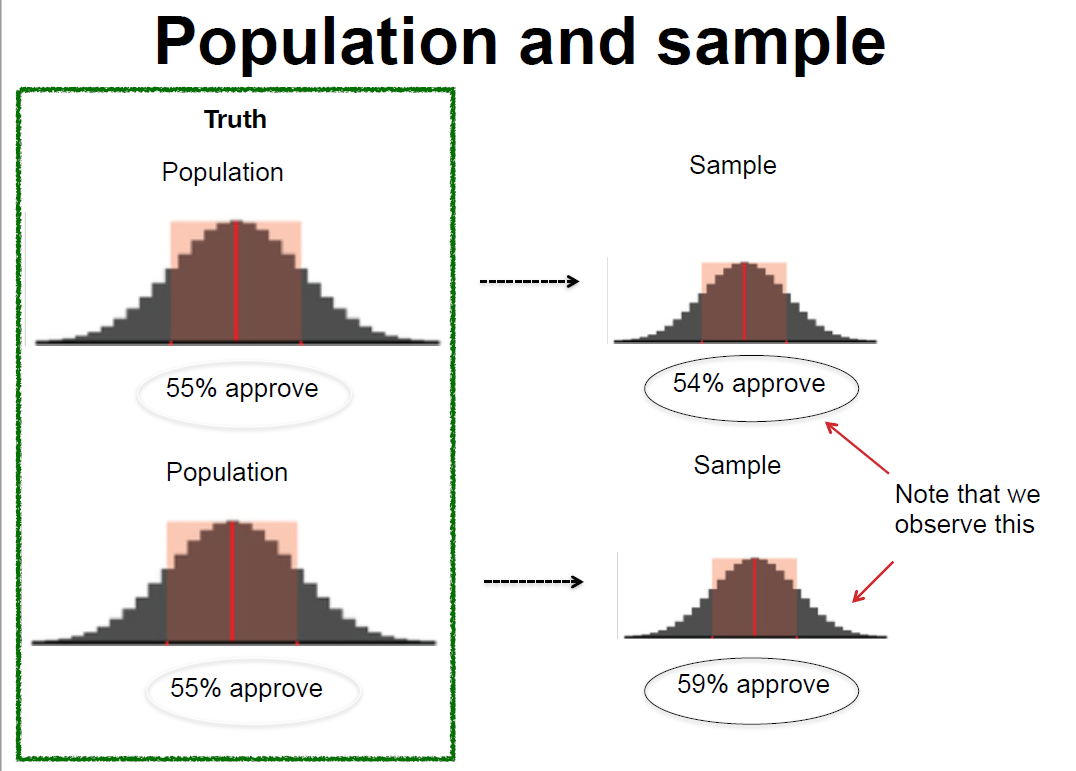
\includegraphics{images/surveys/population_sample.png}
\caption{Population and Sample}\label{fig:population_sample}
}
\end{figure}

A \emph{population} refers to our entire target group that we are trying to
understand. For example, if we are trying to understand how adult Americans
feel about same sex marriage, our population would be U.S. adults. On the
other hand, if we are interested in American college students' opinions about
same sex marriage, then our population would only include college students in
the United States. In drawing the sample, then, researchers must first be
clear about the population that they wish to make inferences about. In order
to get at the population, we often infer from a subset of the entire
population: a sample. A \emph{sample} consists of one or more observations
drawn from the population. Therefore, to draw a meaningful inference about the
population, it is important to have a reliable sample representative of the
population. Ideally, the sample is a miniature version of the population.

\begin{figure}
\hypertarget{fig:Virginia_sampling}{%
\centering
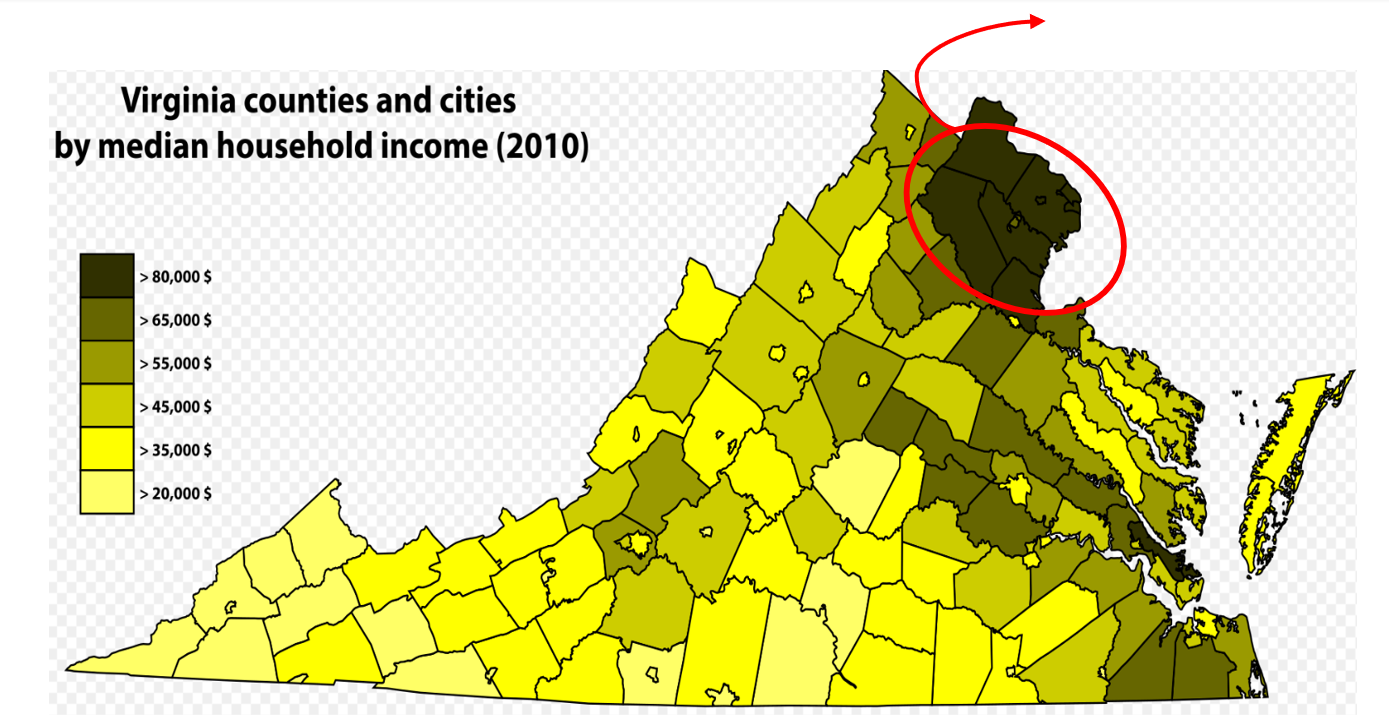
\includegraphics{images/surveys/Virginia_sampling.png}
\caption{How Sampling Can Go Wrong}\label{fig:Virginia_sampling}
}
\end{figure}

Figure 2 presents the map of Virginia counties by median household income. The
upper, darkest counties include some of the richest counties in the United
States, notably Loudoun, Arlington, and Fairfax.\footnote{\url{https://www.worldatlas.com/articles/richest-counties-in-the-united-states.html}}
Interested in American public opinion towards tax policies, let's say that a
professor at George Mason University, located near Fairfax, obtains a
convenience sample of nearby residents (n=50) to conduct a survey about income
property tax. Could you say that the results from this survey reasonably
represent an average American's preferences and opinions about tax policies?

Probably not! As you can see from Figure 2, even within the same state,
counties vary tremendously in their income levels. It is highly likely that
those living in the western-southern part of Virginia are more likely support
higher tax on the rich and more generous welfare benefits. Also, the survey
responses of only fifty people do not provide enough data to render correct
inference about average Americans' attitudes about tax policies. In sum, this
sample of fifty people from the rich Virginia counties is not a miniature
version of the U.S. population. Using such skewed samples prohibits us from
reaching a correct conclusion.

Then how do researchers select samples? Recall from Chapter 4 that there are
two major sampling methods: probability sampling and non-probability sampling.
SRS, stratified sampling, and cluster sampling are all the examples of
probability sampling.

\hypertarget{simple-random-sampling-srs}{%
\subsection{Simple Random Sampling (SRS)}\label{simple-random-sampling-srs}}

Simple random sampling (SRS) is a sampling method to ensure that (1) every
member of the population has an equal probability of being chosen, and that
(2) every combination of N member has an equal chance of being chosen. SRS is
an intuitive and simple technique to extract a sample from the population of
interest. Lottery or random number generator-based sampling is an example of
SRS. If we draw a sufficiently large sample, then we can reasonably assume
that the sample will be somewhat representative of the population (i.e., law
of large numbers). With a large enough sample, random sampling guarantees that
our sample will be like the population on all variables. As a rule of thumb, a
sample size of 1,000 is large enough to make meaningful inferences about
American population.

Then why do we not just always use simple random sampling Why do we have all
these different ways of probability sampling? First, we often face budget
constraints. Or, even though we have enough budgets, our research questions
sometimes dictate that it is better to use other sampling methods than simple
random sampling. For example, there are cases when if we just take the simple
random sample, it is hard to ensure a large-enough observations for certain
groups of people. Then researchers oversample certain subgroups to ensure
sufficient observations to draw meaningful inferences. In exploring the role
of race and ethnicity in political participation in the United States,
Leighley and Vedlitz used oversamples of African Americans, Mexican Americans
and Asian Americans in Texas
(\protect\hyperlink{ref-leighley1999race}{Leighley and Vedlitz 1999}).
Similarly, in examining how racial group categorizations influence
individuals' policy attitudes in the United States, Masuoka and Junn also used
an oversample of Afro-Caribbeans
(\protect\hyperlink{ref-masuoka2013politics}{Masuoka and Junn 2013}).

\textbf{Stratified Sampling}

Stratified sampling differs from SRS in that it first divides the entire
population into smaller homogeneous sub-groups of strata. That is, each
stratum is composed of similar observations -- e.g., based on income,
educational level, race or gender. Then, we take the random samples from each
stratum and pool them together. If we have distinct subgroups based on shared
characteristics, we might use stratified sampling to highlight these
inter-group differences.

\begin{figure}
\hypertarget{fig:stratified-random-sampling}{%
\centering
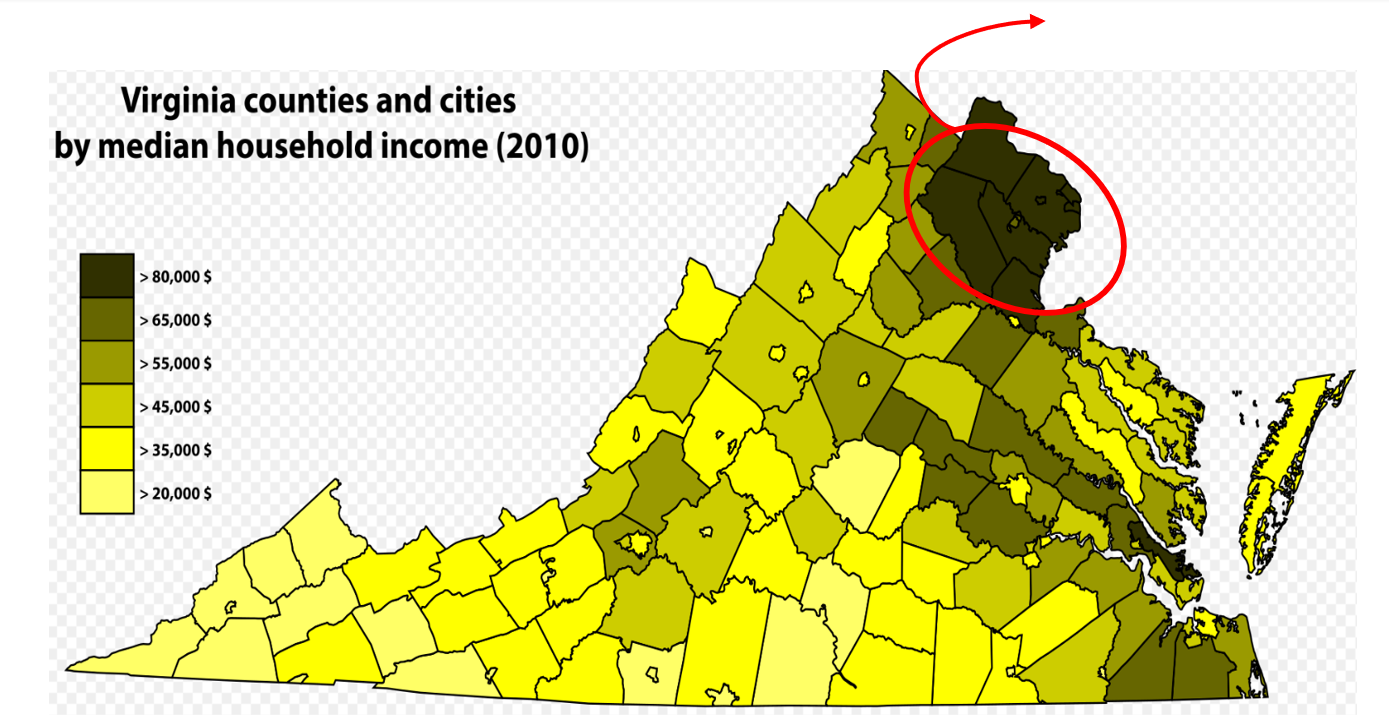
\includegraphics{images/surveys/Virginia_sampling.png}
\caption{Stratified Random Sampling. Note: The population is grouped into
strata based on shared characteristics}\label{fig:stratified-random-sampling}
}
\end{figure}

Because stratification takes into characteristics of the original population,
stratified sampling can better capture the key population characteristics in
the sample. Through stratified sampling, researchers can ensure that certain
subgroups are include in the sample. Moreover, stratification gives a smaller
error in estimation and greater precision than SRS especially when the
inter-group differences are large. For example, in surveying Americans' racial
perceptions and policy attitudes, Masuoka and Junn used stratified sampling to
recruit minority respondents
(\protect\hyperlink{ref-masuoka2013politics}{Masuoka and Junn 2013}), as SRS
possibly would not have guaranteed sufficient number of Asian or Latino
participants. Likewise, YouGov also uses stratified sampling to ensure that
the survey sample resembles the composition of the American population; age,
race, gender and education are typically used as stratification variables.
Cassesse et al.~used YouGov's Cooperative Congressional Election Study, which
used stratified sampling of 50,000 Americans, to examine how white Americans'
racial attitudes affect anti-gender discrimination policy supports
(\protect\hyperlink{ref-cassese2015racializing}{Cassese, Barnes, and Branton
2015}).

Despite its strengths, stratified sampling cannot be used when stratification
is simply impossible -- e.g., when there is very little information available
about the population or when there are only few distinct characteristics (not
enough features) in the population so that we could not divide it into various
subgroups.

\textbf{Cluster Random Sampling}

\begin{figure}
\hypertarget{fig:Cluster-sampling}{%
\centering
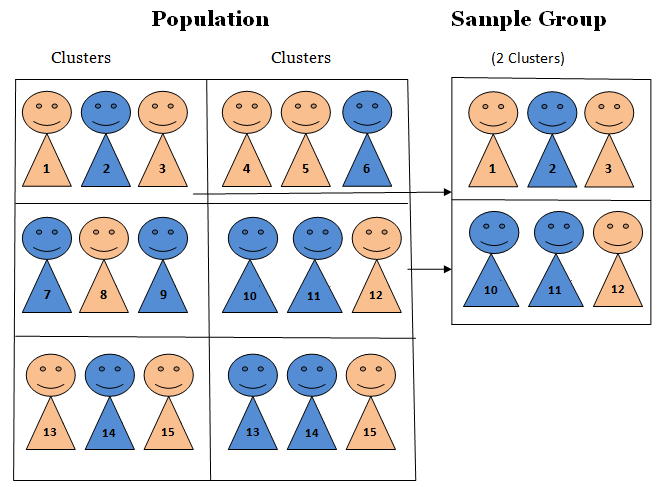
\includegraphics{images/surveys/Cluster-sampling.png}
\caption{Cluster Sampling. Note: Here, the population is divided into several
clusters; note that the entire cluster is sampled}\label{fig:Cluster-sampling}
}
\end{figure}

As in stratified random sampling, the population is divided into sub-groups,
this time called clusters. Unlike strata, however, clusters are not made up of
homogeneous observations. After clustering the population into various
subgroups, we now take the random sampling of the groups (i.e., clusters). In
cluster sampling, each cluster is treated as the sampling unit; in other
words, sampling is done on clusters. Therefore, all the observations in the
cluster are selected in the sample.

The biggest advantage of cluster sampling is that it is relatively cheap and
easier to implement. Intuitively, it is cheaper and easier to observe the
units in a cluster (e.g., based on geography -- like a town or a city) than
observe the sample dispersed across the state. Also, unlike stratified
sampling where researchers are required to have enough information about the
population, cluster sampling can be used even when we cannot obtain sufficient
information about the population as a whole. For example, it would be
tremendously costly or even impossible to construct a complete list of the
entire college undergraduates in the United States. However, it would be
possible to randomly select a subset of the population based on geographical
unit -- e.g., by states, by cities, etc. -- and then conduct surveys on them.
Moreover, as we survey more clusters, we can accumulate the results to get at
the knowledge about the target population; that is, cluster sampling permits
accumulation of samples.

Nevertheless, compared with SRS or stratified sampling, cluster sampling has
the largest possibility of generating biased/skewed samples. Depending on how
you cluster the population, cluster sampling can result in a sample that does
not adequately represent the population. For example, suppose that you are
interested in Illinois residents' opinion towards free trade. Because of the
constraints in time and budget, you did cluster sampling; the clusters you
surveyed were from Evanston and Winnetka (a wealthy town located at the
northern part of Evanston). Can we be confident that our results well
represent the opinion of the entire Illinois residents? Probably no! Chances
are, those clusters might have included one of the wealthiest and/or
best-educated people in Illinois.

Alternatively, we might choose to use non-probability samples.
\textbf{Convenience samples} are a notable example. Rather than being a
representative subset of the population, a convenience sample simply consists
of the cases that are easily available. Our political science department's
research pool, made up of Northwestern undergrads taking political science
courses, is an example of a sample of convenience.

Compared with probability samples, convenience samples provide a relatively
cheaper and easier access to survey implementation. For this reason, before
they field the experiment on a representative sample, researchers often
``pilot'' their survey on convenience samples to figure out whether there are
errors, or logistical and administrative problems in the survey design and
implementation.

Nevertheless, researchers should keep in mind that convenience samples tend to
be skewed -- e.g., student samples are more liberal, largely Democrats and
more politically aware compared to the entire American adults. Likewise, since
these samples are most likely not representative of our population of
interest, we cannot say that survey results from convenience samples provide
accurate insights about the population of interest.\footnote{For more
  discussion, see (\protect\hyperlink{ref-druckman2011students}{Druckman and
  Kam 2011})}

\textbf{Check-in question:} what is probability sampling? Is probability
sampling better than non-probability sampling? What are the pros and cons of
each probability sampling method?*

\hypertarget{fielding-the-survey}{%
\subsection{\texorpdfstring{\textbf{Fielding the
Survey}}{Fielding the Survey}}\label{fielding-the-survey}}

Now off to implementing the survey! Traditionally, surveys have been conducted
via mail, over (landline) phone, or in person. Although these platforms are
still being used, with the wide reach of the Internet, we are now able to
implement surveys more cheaply and effectively online.

Each survey method has its own pros and cons. The methods where a surveyor is
involved in implementation are usually more expensive but have higher response
and completion rates, whereas self-administered surveys are cheaper but may
have lower response and completion rates. Researchers should decide how to
implement their surveys given their research questions, population and sample,
and each method's tradeoffs. Is our biggest expected problem respondent
fatigue or low response rates? Who is our target population: e.g., Chicago
residents or all Americans nation-wide? How big is our budget? If the response
rate is a bigger problem than budget constraint, then we might consider
employing trained surveyors; if our surveys contain questions touching upon
sensitive information, then we might want to employ a method to better ensure
anonymity.

\textbf{Face-to-Face Survey}:

\begin{itemize}
\item
  \uline{Pros}: because this implementation method involves personal
  interactions, it yields higher response and completion rates. Also,
  researchers can monitor/observe participants and ensure that respondents
  followed the instructions. It is also easier to make sure that respondents
  understood the questions. Moreover, this method is particularly suitable if
  we want to include a specific set of sample -- e.g., the elderly, the
  disabled, or the illiterate who cannot easily access to online surveys.
\item
  \uline{Cons}: because it involves the interaction between the respondents
  and the interviewer, the principle of anonymity is compromised. Therefore,
  it is more prone to social desirability bias. Also, compared with
  self-administered surveys, this method is more expensive and logistically
  harder to administer. If the sample is geographically dispersed, researchers
  need extra coordination to implement a face-to-face survey.
\end{itemize}

\textbf{Telephone Survey}

\begin{itemize}
\item
  \uline{Pros}: along with face-to-face surveys, telephone surveys also have
  higher response rates and completion rates than self-administered mail
  surveys. Compared with face-to-face surveys, telephone surveys provide
  better anonymity because respondents do not have to directly meet the
  implementer.
\item
  \uline{Cons}: as the survey is implemented via phone, it is not suitable for
  lengthy surveys. Also, respondents included in the sample might simply
  choose not to pick up the call -- leading to lower contact rates.
\end{itemize}

\textbf{Online Survey}

\begin{itemize}
\item
  \uline{Pros}: even via online, researchers can employ various sampling
  methods -- e.g., SRS or stratified sampling. Through online, we can also
  reach out to a huge sample quickly and cheaply; moreover, we are able to
  reach out to the sample widely dispersed. It guarantees better anonymity
  because respondents do not have to personally face the interviewer (and
  often, they are given de-personalized identification numbers). Researchers
  can get creative with the survey -- online surveys allow researchers to
  include audiovisual components more effectively.
\item
  \uline{Cons}: because it is a self-administered survey, researchers are not
  able to monitor the compliance and the completion of the question. Fatigued
  respondents might just give ``straight-line'' answers. The quality of
  responses might not be as great as that from a face-to-face survey or a
  telephone survey. Also, online survey requires access to a website and
  computer literacy, yielding the net sample of ``computer-literate people.''
  Often, old, disabled people may not be able to conduct the survey.
\end{itemize}

\textbf{Mail Survey}

\begin{itemize}
\item
  \uline{Pros}: as with an online survey, a mail survey also guarantees better
  anonymity than face-to-face surveys. It is relatively easy to administer;
  researchers send out mails with questionnaires, and after completing them
  respondents send those back. Also, respondents can take the survey at their
  own pace; computer-illiterate participants can take the survey as well.
\item
  \uline{Cons}: mail surveys take longer than other methods, and it has low
  response rates as well. There are limitations to employing audio-visual
  materials unlike as in online platforms.
\end{itemize}

\textbf{Check-in question:} suppose that we are interested in how the elderly
(65 years and older) think about universal healthcare. We are interested in
how political liberal-conservative ideology of the elderly is correlated with
their support for universal healthcare. How would you field the survey, and
why?

\hypertarget{analyzing-the-results}{%
\subsection{\texorpdfstring{\textbf{Analyzing the
Results}}{Analyzing the Results}}\label{analyzing-the-results}}

In analyzing the survey results, we must keep in mind that we are trying to
estimate \textbf{parameters} about the population with sample
\textbf{statistics}.\footnote{As you recall, a measurable characteristic of a
  \emph{sample} is called a \textbf{statistic}. A measurable characteristic of
  a \emph{population} is called a \textbf{parameter}.} Because of the
potential errors stemming from the sampling process, we cannot be sure the
sample statics are exactly identical to population parameters. Hence, it is
necessary to build uncertainty in our inference about parameters.

\textbf{Margin of error} quantifies the random sampling error. We cannot be
one hundred percent confident that our sample statistic is the exact value of
the population parameter; because we are using samples, any survey or poll
will differ from the true population by a certain amount. Therefore, by
constructing a \textbf{confidence interval} around a point estimate (i.e.,
sample statistic), we are acknowledging that there is room for error for our
estimates. Margin of error is the range of values below and above the sample
statistic in a confidence interval.

Confidence interval = sample statistic \(\pm\) margin of error

\begin{figure}
\hypertarget{fig:Marginoferror}{%
\centering
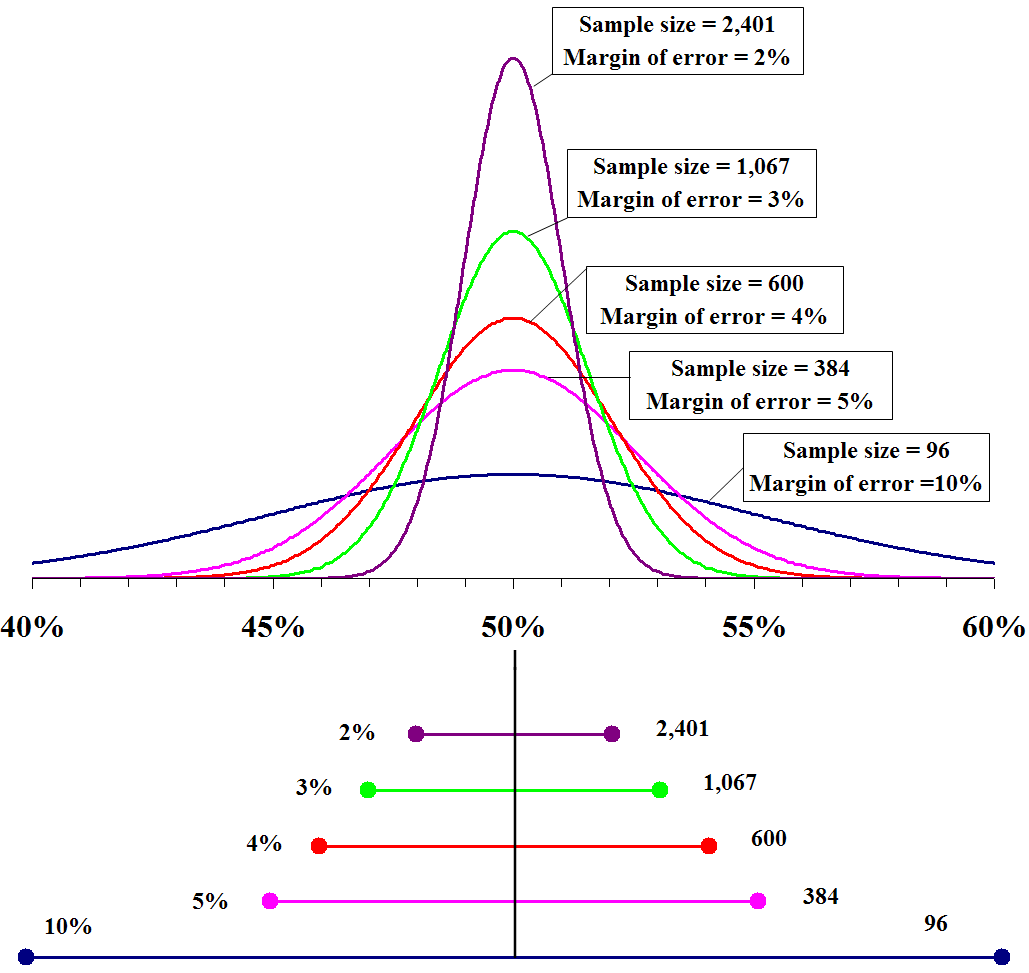
\includegraphics{images/surveys/Marginoferror.png}
\caption{Margin of Error and Confidence Interval}\label{fig:Marginoferror}
}
\end{figure}

As we have seen in the hypothesis testing chapter, confidence intervals mean
that we are confident that the true parameter lies within that range.
Conventionally, political scientists use 95 percent confidence level; this
means that 95 percent of the time, the value obtained from a random sample
will fall within this interval. Note from the Figure 5 that the margin of
error gets smaller with a bigger sample.

\begin{figure}
\hypertarget{fig:Confidence_interval}{%
\centering
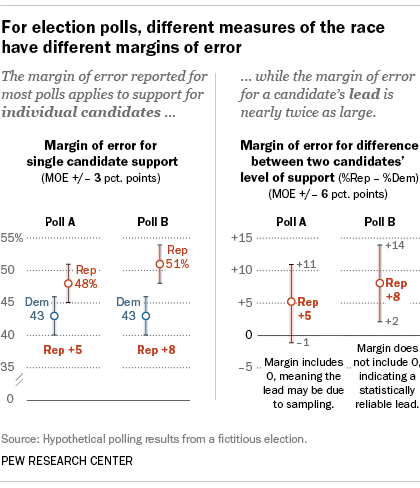
\includegraphics{images/surveys/Confidence_interval.png}
\caption{Confidence Interval in a Poll}\label{fig:Confidence_interval}
}
\end{figure}

\textbf{Check-in question:} Can we say that the Republican candidate is
leading based on the two polls presented in Figure 6? If so, why? If not, then
why not?

We have seen that margin of error takes random sampling error into account;
however, margin of error and confidence interval do not account for systematic
measurement error or systematic sampling error
(\protect\hyperlink{ref-barakso2013understanding}{Barakso, Sabet, and
Schaffner 2013}). Even if we took a random sample of the population, some
subgroups might be overrepresented in the sample -- e.g., Mechanical Turkers
tend to be younger, more college-educated and liberal than average Americans.
Or, because of the way the survey was implemented, there might be non-response
errors -- e.g., if we conduct an online survey, the elderly might be
undersampled. In such cases, treating all the responses from an
unrepresentative sample equally might lead to a failure to have a correct
inference about the population.

\textbf{Weighting} is a technique to correct for the sample's lack of
representativity. Data can be weighted by various variables such as age,
gender, race/ethnicity, or income, so that the sample could resemble the
population, and ultimately, get at a more accurate population parameter.

\hypertarget{applications-1}{%
\section{Applications}\label{applications-1}}

We can see surveys everywhere. Companies conduct surveys for market research
and customer satisfaction; newspapers and think tanks run surveys to see what
the public thinks about different issues and policies.

Surveys can be large -- as in ANES (American National Election Studies), GSS
(General Social Survey), WVS (World Value Survey) and Eurobarometer. These
surveys ask questions ranging from respondents' values, life goals, to
political and social issue salience, and to basic demographics. With the
extensive lists of questions, these survey data can provide us with
quasi-qualitative data about respondents. Similarly, WVS asks what respondents
value as important qualities of a child, desirable traits of neighbors,
essential features of democracy, and how much confidence they have in various
institutions (e.g., Labor Unions or the Police), religiosity, etc\footnote{Because
  the same questions are asked in different countries around the same time
  frame, it allows us to compare what people value and how people think in
  various countries. You can access to WVS here:
  \url{http://www.worldvaluessurvey.org/wvs.jsp.}}. We can often see political
science and sociology works employing these surveys; Kane and Whipkey, for
example, use the General Social Survey to reveal the motivations behind the
support for gender-related affirmative actions
(\protect\hyperlink{ref-kane2009predictors}{Kane and Whipkey 2009}).

Surveys can also be small, often as in polls. Note that by a ``small" survey,
social scientists are not referring to a survey with a small sample size but
one with few questions. Gallup's presidential approval rating
polls,\footnote{\url{http://www.presidency.ucsb.edu/data/popularity.php}} for
example, has only one question! Such short surveys, often with just one or two
key question(s), are called polls rather than surveys. Pew Research Center
conducts polls for various topics, which are widely used in academic works and
also quoted in the media.

\hypertarget{advantages-of-method}{%
\section{Advantages of Method}\label{advantages-of-method}}

A lot of political science theories are based on micro-level foundations.
Political scientists are interested in uncovering how individuals think and
feel about certain policies and social phenomena, and why they think so.
Surveys are valuable for empirically examining these theories, since they
allow the direct measure of public opinion and individual-level variables. For
example, as Open Economy Politics scholars predict, does relative economic
standing of an individual affect his/her attitudes toward free trade? Or are
there more than mere economic factors, such as gender or socialization via
labor unions, that determine trade policy preferences? Surveys allow
researchers to directly investigate these research questions.

The use of surveys is not limited to asking respondents about their policy
preferences or political ideology. Instead, surveys also allow us to explore
various topics. GSS and WVS (as explained above) are notable examples -- the
range of questions asked is very wide; we can ask respondents' moral values,
environmental concerns, policy preferences and their issue salience via
surveys. Moreover, standardized surveys over a long period of time can provide
a valuable resource for time trend analysis.

Especially with the advancement of online survey platforms, surveys are often
relatively easy -- despite all the considerations to be taken before actually
implementing the survey -- to field. Researchers are able to reach out to a
large number of respondents with fewer geographic limitations. Furthermore,
compared to other data collection methods (e.g., in-depth interviews, case
studies, archival research), surveys take less time. Moreover, with proper
statistical analytical tools, surveys provide an effective, flexible way of
generating knowledge.

\hypertarget{disadvantages-of-method-surveys-easier-said-than-done}{%
\section{Disadvantages of Method: Surveys, Easier Said than
Done}\label{disadvantages-of-method-surveys-easier-said-than-done}}

However, even a well-designed survey could go wrong -- sometimes for reasons
outside the researchers' control! In addition to errors pertaining to the
sampling stage, there are other potential errors and disadvantages because
surveys involve human responses.

\textbf{\uline{Respondent fatigue}}: Because human beings have limited
attention span, participants might become tired (and/or bored) of answering
the survey questions, and as a result, the quality of their responses
deteriorates. People might just click ``don't know,'' give out random
responses, or simply skip the questions and not answer at all. We can expect
survey respondents to be fatigued especially when the survey questionnaire is
lengthy.

\textbf{\uline{Question wording and order effect}}: Depending on how the
question is asked, respondents might give different answers. Even small
differences in wording can alter the survey results (more in the
\href{./experiments.html}{Experiment chapter} -- framing effect). Pew Research
Center's surveys on American public opinion about the Iraq War provide a good
example. When the question was worded ``would you favor or oppose taking
military action in Iraq to end Saddam Hussein's rule?'', 68\% of participants
responded that they favored military action against Iraq while only 25\%
answered that they are against the military action. When the question was
worded differently -- ``would you favor or oppose taking military action in
Iraq to end Saddam Hussein's rule even if it meant that U.S. forces might
suffer thousands of casualties?'' -- the results changed substantially. Now,
48\% of the respondents said they opposed the military action while only 43\%
said they favored it! Question order can also impact survey results. Schuman
and Presser present an interesting example. In a survey during the Cold War,
Americans were asked whether journalists should be allowed to travel between
the US and the USSR. When they were first questioned whether Soviet
journalists should be allowed to visit the U.S. to write articles for Soviet
newspapers (and then were asked about American journalists), respondents
showed lower support for cross-country travel of both Soviet and American
journalists. However, when they were first questioned regarding American
journalists traveling to the Soviet Union, respondents were more likely to
support the reciprocal travel of Russians and Americans
(\protect\hyperlink{ref-schuman1996questions}{Schuman and Presser 1996}).

\textbf{\uline{Limitation in human capacity to recall}}: People might not
accurately recall past events, and simply because they failed to properly
recollect the past, it is also likely that respondents could not provide their
actual attitudes or opinions.

\textbf{\uline{Conflict of incentives}}: Nowadays, researchers can easily
recruit survey participants via online platforms such as Amazon Mechanical
Turk (MTurk). These respondents are paid per task completed; therefore, their
interests lie in maximizing the number of surveys completed. Contrary to the
researchers' incentives to ensure well-contemplated responses, these online
survey platforms can encourage respondents to finish surveys as quickly as
possible and move on to the next tasks, resulting in low-quality answers.

\textbf{\uline{Social desirability bias}}: Respondents may also be pressured
to answer questions in a manner that will be viewed `favorably' by others. A
famous example for social desirability bias is that when asked about the
number of their sexual partners, women tend to attenuate their numbers while
men tend to inflate theirs. Since health-related studies often rely on
self-reported measures, it inevitably suffers social desirability
bias\footnote{Van der Mortel (2008) finds that social desirability-motivated
  responses were present in approximately 43\% out of 14,275 health studies
  (\protect\hyperlink{ref-van2008faking}{Van de Mortel et al. 2008}).}
Similarly, family planning is an area vulnerable to this bias; people tend to
underreport the frequency of unprotected sex while overprotecting the
contraceptive use (\protect\hyperlink{ref-stuart2009social}{Stuart and Grimes
2009}). They also found that people extensively underreport induced abortion.
Hadaway et al.~revealed that church attendance rates based on respondents'
self-reported responses substantially overstates actual religious attendance
in the U.S. (\protect\hyperlink{ref-hadaway1993polls}{Hadaway, Marler, and
Chaves 1993}). To mitigate social desirability bias, anonymous
self-administration (e.g., via the Internet) might help -- it can ensure that
respondents do not feel directly and personally involved, and can decrease
social desirability bias. Researchers can also emphasize that the responses
will be kept confidential and anonymous and that the responses therefore will
not be used against the respondents \footnote{On the other hand, some studies
  find that social desirability bias does not significantly affect the
  conclusion. Heerwig and McCabe find no evidence the college-educated
  people's support for a black president were inflated due to social
  desirability bias (\protect\hyperlink{ref-heerwig2009education}{Heerwig and
  McCabe 2009})}.

By nature, a survey is a \textbf{\uline{large-N, observational study}};
in-depth exploration of the motivations behind the answers could not simply be
observed via survey. Interviews might be more appropriate in this case.
Alternatively, we can add open-end questions in the survey to ask ``why''
questions which would require other analyses such as text and/or content
analysis. \textbf{Inter-coder reliability} is especially important for content
analysis of open-end responses. Inter-coder reliability is the widely used
term for the extent to which independent coders evaluate a characteristic of a
message or artifact and reach the same conclusion
(\protect\hyperlink{ref-lombard2002content}{Lombard, Snyder-Duch, and Bracken
2002}). For example, surveys such as ANES often ask respondents why they
support certain candidates over others. Respondents provide various reasons
for supporting specific candidates, and it is necessary to sort out what the
most salient reasons are for the respondents. Inter-coder reliability in this
context refers to the extent to which different coders classify the content of
the answers into the same category. It is a critical component of content
analysis -- when it is not established, the data and interpretation of the
data cannot be considered valid
(\protect\hyperlink{ref-lombard2002content}{Lombard, Snyder-Duch, and Bracken
2002}).

\textbf{\uline{Non-response bias}}: When respondents differ from
non-respondents in meaningful ways. Unlike coverage bias, non-response bias
occurs when some respondents included in the sample do not respond. This might
be because the respondents refuse to participate, or the researchers failed to
reach some participants. For example, if you are running a survey about
immigration and assimilation, and if your survey includes a question about
respondents' legal status, it is highly likely that those who are undocumented
would feel more uncomfortable filling out the survey and therefore, more
likely to opt out. Although the research question was about how both
undocumented and documented immigrants and their assimilation patterns, this
survey will result in a net sample of legal/documented immigrants (which is
different from the original sample). As expected, surveys asking for legally
sensitive information are more sensitive to non-response bias; also, if the
survey explicitly states that the government or organizations of authority are
collecting the data, we might face more serious non-response bias.

\textbf{\uline{Coverage error}}: This error occurs when there is not a
one-to-one correspondence between the target population and the sampling frame
from which a sample is drawn. A Sampling frame is the list of all the units
within a population that could be sampled. It could include not only
individuals, but also households, schools, companies or other institutions
depending on our research question and unit of analysis. Ideally, the sampling
frame perfectly coincides with the target population; but when it does not
coincide, we have coverage error.

\begin{figure}
\hypertarget{fig:coverage_error}{%
\centering
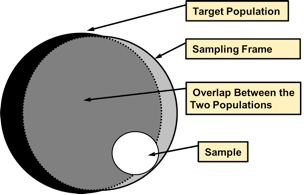
\includegraphics{images/surveys/coverage_error.png}
\caption{Coverage Error}\label{fig:coverage_error}
}
\end{figure}

\textbf{Check-in question:} what could be the solutions to social desirability
bias or non-response for sensitive questions included in the survey? Be
creative!

\hypertarget{broader-significanceuse-in-political-science-2}{%
\section{Broader significance/use in political
science}\label{broader-significanceuse-in-political-science-2}}

When and how will we encounter surveys in political science? Almost all
subfields -- ranging from American Politics to International Relations -- in
political science have adopted survey research as their empirical strategy.

\textbf{1. Use in IPE: What Determines Individual Support for Economic
Openness?}

International political economy (IPE) theorists, for example, use surveys to
show the determinants of individuals' economic policy preferences. Using
cross-country surveys for Asian and European countries, Mayda et al.~find that
if individuals perceive risk (or instability) to increase along with trade
openness, (s)he favors more restrictive policies such as tariffs or quotas.
Using the same survey data, they also find that ideational factors, such as
nationalism, also matter in determining individuals' trade protectionism
(\protect\hyperlink{ref-mayda2007risk}{Mayda, O'Rourke, and Sinnott 2007}). In
a similar vein, also using survey data, Mutz and Kim find that in-group
favoritism influences Americans' attitudes toward international trade
(\protect\hyperlink{ref-mutz2017impact}{Mutz and Kim 2017}). Rather than
maximizing their own pocketbook gains, Americans tend to choose policies that
maximize the well-being of fellow Americans. They also find that when
Americans think that the trading partner country loses so that the U.S.
achieves a greater relative advantage, trade policy garners greater support.

\textbf{2. Use in American Politics}

American politics scholars also use survey to study public opinion. For
example, to reveal factors driving Trump's electoral success in 2016, Ferguson
et al.~also use survey data (ANES); they find that (unsurprisingly) Trump's
populist rhetoric resonated with Americans' economic concerns, racism and
sexism. They reveal that the roots of Trump's victory in 2016 lie in
Americans' economic and social concerns
(\protect\hyperlink{ref-ferguson2018economic}{Ferguson et al. 2018}).

\textbf{3. Use in Everyday Politics}

In addition to their academic uses, surveys are also used for our everyday
lives. Because their professional careers depend on reading public opinion
accurately, politicians refer to various polls to grasp the public's attitudes
toward current policies and future policy options
(\protect\hyperlink{ref-erikson2015american}{Erikson and Tedin 2015}). The
American public is becoming more engaged in politics, leading them to
increasingly follow the polls more closely.\footnote{In 1944, only 19 percent
  of Americans said they regularly or occasionally followed poll results; this
  figure rose to 41 percent by 1985, to 65 percent in 2001, and to 89 percent
  in 2008 (\protect\hyperlink{ref-erikson2015american}{Erikson and Tedin
  2015}).} As they write, ``academic polls advance our knowledge of public
opinion, and commercial pollsters satisfy the public's (and private clients')
curiosity regarding trends in public opinion.''

\hypertarget{conclusion-4}{%
\section{Conclusion}\label{conclusion-4}}

A lot of political science theories are either explicitly or implicitly based
on micro-level foundations. Surveys provide a good means to directly probe how
individuals think, allowing the empirical testing of political science
theories. With the same survey questions repeatedly asked over a long time,
surveys can provide insights about the trends in the public opinion. Surveys
are also very versatile; they can be combined with other data collection
methods and analysis techniques such as experiments and regressions. Surveys
are important for politicians as well, since they rely on surveys/polls to
base their electoral strategies and policy platforms. However, as social
scientists, we should also remember that although the idea of survey research
seems very intuitive, a good survey is surprisingly hard to design and
implement as we have seen in this chapter. Errors can arise at every stages of
survey design, and only with caution can we reap the full benefits from a
survey research.

\hypertarget{application-questions-4}{%
\section{Application Questions}\label{application-questions-4}}

\textbf{1. True or false?}

\begin{itemize}
\tightlist
\item
  Surveys offer better external validity than experiments.
\item
  Surveys offer better external validity than case studies.
\item
  Surveys are particularly good at exploring subgroup differences and
  historical trends because they usually have large enough sample sizes.
\end{itemize}

\textbf{2. Define and provide an example of each of the following errors.}

\begin{itemize}
\tightlist
\item
  Sampling error
\item
  Non-response error
\item
  Measurement error
\end{itemize}

\hypertarget{key-terms-3}{%
\section{Key Terms}\label{key-terms-3}}

\begin{itemize}
\tightlist
\item
  conceptualization
\item
  convenience sample
\item
  coverage bias
\item
  double-barreled question
\item
  inter-coder reliability
\item
  margin of error
\item
  non-response bias
\item
  response rate
\item
  sample
\item
  sampling frame
\item
  validity
\item
  weighting
\end{itemize}

\hypertarget{answers-to-application-questions-4}{%
\section{Answers to Application
Questions}\label{answers-to-application-questions-4}}

\textbf{True or false question:} True, True, False

\hypertarget{experiments}{%
\chapter{Experiments}\label{experiments}}

\textbf{By S.R. Gubitz}

\hypertarget{introduction-5}{%
\section{Introduction}\label{introduction-5}}

Perhaps you have wondered what might have happened along a path you did not
take. Or perhaps you have speculated about how differently history would turn
out if some key event did not occur the way it did in reality. For example, if
the Supreme Court of the United States in 2000 had allowed presidential
election recount efforts to continue in Florida, might Al Gore have beaten
George W. Bush to become president? Or, if you had not skipped breakfast this
morning, might you feel a little less groggy right now? In practice, a path
not taken is the same as one that never existed; we do not get to run history
twice like a computer simulation to observe the path not taken. But, in some
scientific contexts, you can observe both paths at once. This is the nature of
an experiment; we get to cheat history, time, and space to observe the
otherwise un-observable.

Political science finds experiments especially useful, because oftentimes the
path not taken has serious political or societal ramifications. For example,
what happens to voter turnout rates when political parties decide to ignore
communities of color, and what might happen if they do not? In politics, many
wish that they can turn back the clocks and run history twice. In political
science, that is sometimes entirely possible in an experimental research
design.

\hypertarget{background-1}{%
\section{Background}\label{background-1}}

The first recorded experiment occurred in 1835, in Nuremberg, Germany
(\protect\hyperlink{ref-jamison_entry_2019}{Jamison 2019}). The researchers
conducting this experiment were interested in the effects of a certain
homeopathic medicine: the inclusion of small amounts of salt in water. The
researchers divided 100 local residents into a treatment group of 50 that
received salt in a vial of water, and a control group of 50 that only received
a vial of water. Participants were later examined to see the effect of the
salt water on any physical ailments; the researchers found that the
intervention had no effects.

It took nearly 100 years for political science to attempt its first recorded
experiment (although the discipline was fairly new at the time, having just
split off from history and economics). Harold Gosnell conducted an experiment
around the 1924 US presidential election to test the effects of mailed
postcards on voter turnout
(\protect\hyperlink{ref-gosnell_getting_1927}{Gosnell 1927}). Gosnell sent out
postcards to certain wards, randomizing which half of the ward would get the
postcards and which would not. He found modest effects, setting the stage for
future work on randomized get-out-the-vote (GOTV) efforts.

But Gosnell's work was not immediately appreciated by political scientists,
and it took nearly another 60 years before serious experimental work began to
be taken seriously in the discipline. Shanto Iyengar, Mark Peters, and Donald
Kinder invited participants to watch television news programs at the
University of North Carolina, Chapel Hill
(\protect\hyperlink{ref-iyengar_experimental_1982}{Iyengar, Peters, and Kinder
1982}). What the participants did not know, however, is that they were
randomly assigned to watch some newscasts that had been edited to emphasize
certain stories over others. These manipulations resulted in the control group
assessing the president's performance differently, based on the issues they
were exposed to in the television news program.

And from that point, experiments began steadily becoming a mainstay research
method in political science. The figure below shows the number of experiments
published every year in the \emph{American Political Science Review}, one of
the top publications in political science. As the figure shows, following
Iyengar, Peters, and Kinder's work in the 1980s, experiments started to be
published in this journal at an increasing rate. However, it is important to
keep in mind that experiments are not even close to being the dominant
research method. If you have already read in the chapter on \emph{surveys},
then you already know a good deal about the most dominant quantitative
research method: surveys.

\begin{figure}
\hypertarget{fig:trend}{%
\centering
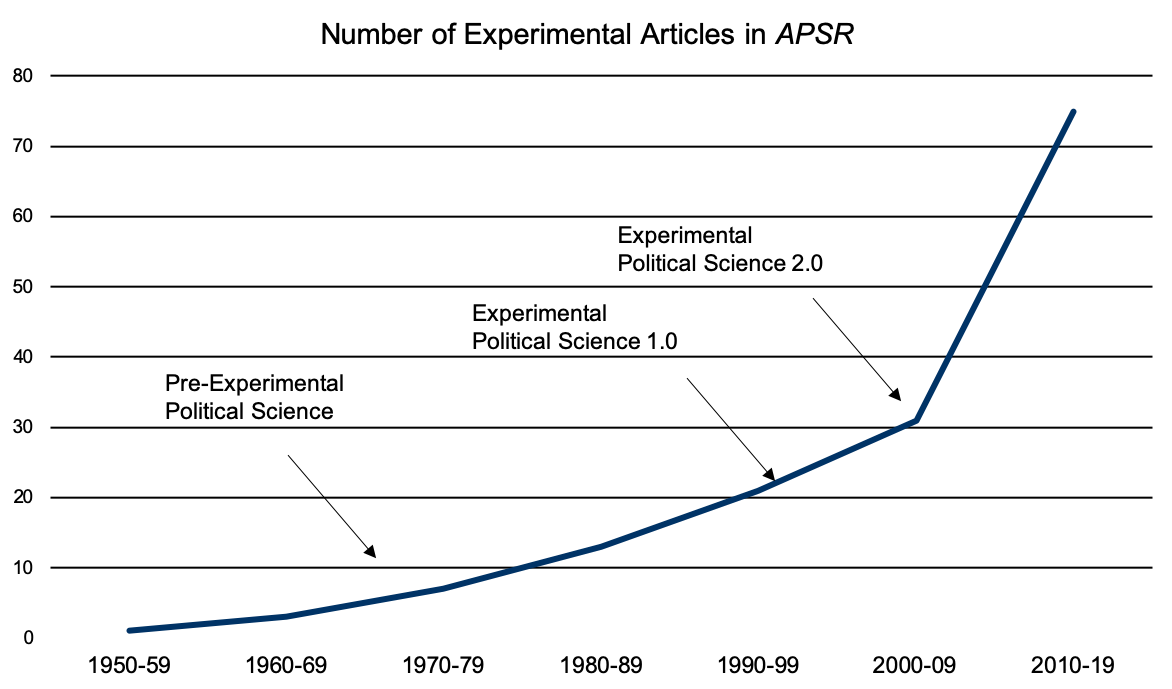
\includegraphics{images/trend.png}
\caption{totals are aggregated per decade}\label{fig:trend}
}
\end{figure}

\hypertarget{method-setupoverview}{%
\section{Method: setup/overview}\label{method-setupoverview}}

Experiments, or RCTs (randomized control trials) as they are often called,
involve the randomized assignment of individuals into one of two groups (in
the most basic design): a \textbf{treatment group} that receives some
intervention; and a \textbf{control group} that does not. This design allows
the researcher to determine the effect of some intervention (e.g.,
individualized tutoring) by comparing the value of some outcome (e.g., test
scores) in the treatment group to the control group that did not receive the
intervention. Do note, however, that most experiments have several treatment
groups and some even have several control groups depending on to what they
need to make their comparison.

It is important to differentiate the random assignment necessary to conduct an
experiment from the random sampling you learned about in the chapter on
\emph{surveys}. In that chapter, it was explained that random sampling is when
you randomly select individuals from some population you are interested in
studying to be a part of your survey. But random assignment has nothing to do
with that sampling technique. Rather, random assignment means taking your
sample, however it was collected, and randomly assigning them to your
treatment group(s) or control group(s). This random assignment is necessary to
ensure that the treatment and control groups have nearly the same odds of
being comparable to each other in terms of demographic characteristics of your
overall sample. So, if you have 50 African Americans in your sample of 250
people, and you have four treatment groups and one control group, then random
assignment should result in groups of near 50 people each, with 10 African
Americans per group.

A consequence of this requirement that the sample be randomly assigned to
experimental groups means that how the sample was collected is less important.
This, again, is a deviation from what you learned about surveys earlier in
this book, where sampling mattered a great deal. But a good experiment can
rely on what is called a \textbf{convenience sample}, or a sample that is made
up of easy to reach people. For instance, for much of the 20th century,
researchers often placed newspaper advertisements to construct their samples.
Nowadays, however, there are entire online services built around getting
researchers participants for their experiments. But these convenience samples
do not undermine the legitimacy of the experiment, unless the researchers are
trying to generalize to a certain population. If you had a convenience sample
of your friends and family, you would be hard pressed to say that any results
from an experiment on that sample could generalize to the population of a
country.

\begin{shaded*}

\textbf{Check-in Question 1:} Is "random assignment" another way of saying
"random sampling" and vice versa? If not, how are they distinct from one
another?

\end{shaded*}

\hypertarget{method-detail-types-of-experiments}{%
\section{Method: detail (types of
experiments)}\label{method-detail-types-of-experiments}}

As you can probably gather from the few examples provided so far, there are
many different types of experiments. Each offer their own unique way of
answering certain scientific questions that the others cannot. In the
following sections, we will review four types of experiments and example from
political science for each.

\hypertarget{surveys-vs-survey-experiments}{%
\subsection{Surveys vs Survey
Experiments}\label{surveys-vs-survey-experiments}}

The growth of online survey platforms, such as Survey Monkey and Qualtrics,
have resulted in a similar growth in the use of survey experiments. While you
might already be familiar with surveys, it is important to differentiate
survey experiments. That is, \textbf{survey experiments} are experiments that
are embedded in surveys. Within such a survey, participants answer questions
and read materials just as they would in any survey. But at some point,
respondents are randomly assigned to a treatment or control group.

What is advantageous about experiments embedded in a survey like this is that
it is extremely easy to do. Because the surveys are often disseminated online,
that means the researcher does not need a physical space where the experiment
will be administered. Further, survey respondents are quite easy to obtain
while providing modest compensation. Survey firms like YouGov provide samples
to respond to researcher-provided surveys for a few dollars a respondent; the
samples can even be constructed in ways that resemble national
representativeness without true random sampling. For the more-frugal
researchers, survey experiments can be administered on Amazon's Mechanical
Turk (MTurk) service, which people perform various tasks online for monetary
compensation; these are usually menial tasks like testing website functions.
But, in recent years, political scientists have been using MTurk to
disseminate their survey experiments, as the service is far more affordable
than a professional survey firm.

For all of its advantages, survey experiments suffer from the limitations of
their medium; that is, a researcher can only craft treatment interventions
that can be disseminated via survey materials. Oftentimes, this means
text-based treatments that require the respondent to read (a burden that any
undergraduate student can sympathize with); this can be troublesome when the
researchers cannot prove the respondents read the treatment text, leading to
false conclusions about the effectiveness (or lack thereof) of the experiment.
Also, survey experiments rely on self-reported outcomes to draw their
conclusions, which means that the respondent was allowed to report how they
felt or thought at that time. This is problematic if there is greater
incentive to not be entirely forthcoming on the survey, or if people are
simply bad at assessing certain psychological states (e.g., "how angry are you
right now on a scale of 1-7?").

For example, Dingding Chen, Chao-yo Cheng, and Johannes Urpelainen
(\protect\hyperlink{ref-chen_support_2016}{Chen, Cheng, and Urpelainen 2016})
study how different ways of framing renewable energy in China affected Chinese
citizens' support for such programs. They disseminated a survey online to over
2,000 Chinese citizens collected by a professional company (i.e., this was a
convenience sample). Respondents were assigned to one of eight groups (six
treatment, two control) that varied the argument being used to support or
oppose greater investment in renewable energy in China. They measured support
for greater investment on a 1-5 scale, with 5 being the highest support. The
researchers find that support was at its highest when respondents were exposed
to a frame that presented greater investment in renewable energy as a means of
energy security, rather than as a means of combating global warming or air
pollution.

While this finding is only possible thanks to an experimental design, it is
also only feasible with the sample size they had (n = 2,000) because of how
cheap and efficient survey experiments can be. But, we should ask whether or
not the weaknesses of survey experiments harmed the study in question. For
instance, since support for renewable energy was self-reported, might there
have been some degree of bias toward greater support, regardless of the
respondents' true feelings? But, because this is a survey experiment, we can
never be entirely sure that the respondents were truthful in their responses.
But simply, survey experiments remove a great deal of control from the
experimenters.

\hypertarget{laboratory-experiments}{%
\subsection{Laboratory Experiments}\label{laboratory-experiments}}

While survey experiments lack control of the environment in which the
experiment takes place, \textbf{laboratory experiments} exercise near-complete
control. These experiments take place in controlled environments, or a
laboratory. Usually, for university professors, this means some room that
their department or university provided for that purpose. But, oftentimes,
labs can be made out of just about any room, so long as the experiment is not
disturbed. In fact, recent research has tried taking mobile labs to
communities that have been traditionally difficult to reach, all in order to
better study and understand those communities and the people living in them
(\protect\hyperlink{ref-neil_a._lewis_studying_2019}{Lewis Jr 2019}).

The greatest advantage of the laboratory experiment is that the researchers
have a greater degree of control than in survey experiments. They can ensure
that treatment is administered correctly, and that the people participating in
the experiment are actually people and not automated survey takers (a serious
concern for some online surveys). Further, while survey experiments are
limited to mostly text-based treatment designs, laboratory experiments can be
far more inventive. One of the classic reasons to conduct a laboratory
experiment is because the research question requires studying some complex
social interaction. A lab allows for researchers to create a physical space in
which they can observe nearly real-life social interaction. And one last
benefit of this method is that researchers can directly observe and record
real behaviors and speech, and are not limited to self-reported attitudes in
the same way survey experiments are.

That being said, the inherent problem with lab experiments is finding the
people to fill the lab. As opposed to ease in which a survey can be filled
out, participants in a lab experiment must actually travel to and from the lab
in order to participate. This may sound trivial, but imagine the difficulty
and expense for some to travel to lab sites. In some international contexts,
lab experiments can be extremely costly because proper compensation must
sometimes cover people's missed wages from a day's work. The end result of
this is that lab experiments usually have rather small sample sizes, usually
somewhere between 100 and 200 participants. Compare that to the thousands of
participants that a survey experiment can garner for roughly the same cost and
you begin to realize the issue with wanting to exercise greater control.
Smaller sample sizes often mean fewer people per experimental group, which
means less statistical power to calculate meaningful effects.

Again, it is worth noting that some questions are answerable in a lab setting.
For example, Ismail White, Chryl Laird, and Troy Allen
(\protect\hyperlink{ref-white_selling_2014}{I. K. White, Laird, and Allen
2014}) conducted a lab experiment two months before the 2012 presidential
election between Barack Obama, a Democrat, and Mitt Romney, a Republican. This
experiment took place in a historically black college/university (HBCU), which
gave the researchers access to a somewhat unique sample of exclusively young
African American living in a Black institution of higher learning. This was a
boon for the study because they were interested in seeing whether economic
self-interest could undermine these young people's partisanship. African
Americans in the United States are largely members of the Democratic Party
(over 80 percent), but these researchers were interested in testing the limits
of this partisan loyalty.

Participants were brought to the lab and instructed after a brief interview to
allocate \$100 between the two candidates running for President, Obama and
Romney. What they did not tell the participants (aside from the money not
actually being donated) was that some were randomly assigned to a cue that
told them that for every \$10 they gave to the Romney campaign, the
participant would receive \$1 for themselves, paid in cash. This meant that
participants in this condition, if they gave all \$100 to Romney, thus
undermining their likely Democratic Party loyalty, they would receive \$10.
But what made this lab experiment unique was the inclusion of another
treatment group, identical to the economic incentive condition, that
stipulated that their donation amounts would be made public in the
university's student newspaper, thus revealing their behavior to their peers;
this is the type of social interaction that is often impractical to replicate
in a survey setting. Ultimately, those in the control group donated an average
of \$90 to Obama, while those in the economic incentive condition's average
was \$68, and those with the additional stipulation had an average of \$86. In
short, because of the lab setting, the researchers could leverage the presence
of a Black institution in the minds of young African Americans to potentially
dissuade them from giving into their economic self-interest.

\begin{shaded*}

\textbf{Check-in Question 2:} What is the primary disadvantage of conducting a
lab experiment, compared to a survey experiment?

\end{shaded*}

\hypertarget{field-experiments}{%
\section{Field Experiments}\label{field-experiments}}

Oftentimes, researchers do not have the liberty of controlling where and when
they want to conduct their experiments. For instance, if you want to conduct
an experiment that tries to increase Asian American voter turnout in Los
Angeles, that means that you necessarily have to conduct the experiment weeks
or months before the election in question. These experiments are what are
called \textbf{field experiments}, or experiments that take place in the
physical location you are interested in studying.

The biggest advantage of this sort of experiment is that sometimes they are
the only option and offer a unique means of gleaning certain information about
the real world. That is, these experiments are much closer to observing real
world behaviors and outcomes than survey and lab experiments, in most cases.
However, a serious downside of a field experiment is that they are incredibly
expensive to run, even more so than a lab experiment. These experiments often
involve many researchers who must be compensated, and treatment materials that
often bear an additional cost than simply an online survey. For instance, even
if you have disseminating a survey in the field, you either have to print it
and collect those finished surveys via pre-paid mail, or bring a tablet device
for participants to use there. Needless to say, the costs quickly add up and
the sample sizes can vary quite a bit depending on available resources.

But in those instances where there is no other option, a field experiment can
find incredible results. For example, Victoria Anne Shineman
(\protect\hyperlink{ref-shineman_if_2018}{Shineman 2018}) conducted a field
experiment in San Francisco, CA during a 2011 local municipal election.
Shineman wanted to study how voter mobilization efforts not only increased
voter turnout, but also voter knowledge. She invited 178 subjects to complete
two surveys, one before the election and one afterward, in exchange for \$25.
It was during the first survey that Shineman randomly assigned participants to
receive different types of mobilization assistance (or none at all for the
control), some of which included the necessary forms to register to vote.
After the election, Shineman found that not only had mobilization been
increased as is typical in these GOTV experiments, but that those exposed to
mobilization efforts also exhibited greater political knowledge than those in
the control, as measured by the second survey conducted after the election.
Without being able to go into the field like this, Shineman could not answer
the question of whether mobilization effects spilled over to political
knowledge, as this would be impossible to glean from just a survey or in a
lab. However, it is worth noting just how expensive this study was for the
researcher; the amount of resources required to conduct a field experiment is
a serious disadvantage.

\hypertarget{natural-experiments}{%
\section{Natural Experiments}\label{natural-experiments}}

The final major type of experiment to review is one that is the most
infrequently used by political scientists, and not for lack of trying.
\textbf{Natural experiments} are experiments that are not exactly conducted by
the researcher; that is, the randomization process necessary to call it an
experiment was done by someone or something other than the researcher. This
could be an "act of God," like a natural disaster's effects on voter turnout,
or a local municipality's property tax's effects on desegregation efforts in
the local school system. No matter how the randomization happened, if it was
not the researcher who did it, then it is a natural experiment.

The advantage of analyzing a natural experiment (again, it is not accurate to
say one "conducts" a natural experiment) is that the outcomes observed could
not be any more realistic. In social science contexts, natural experiments
produce effects on real people in the real world; the stakes are at their
highest. However, there are a whole host of problems that come attached to a
natural experiment. First and foremost, because natural experiments are
conducted by nature or some third party, that means that you have to find the
natural experiments that have already happened. This entails identifying the
cause, some manner of measuring who was affected by the cause, and some manner
of measuring the outcomes you are interested in. If any of that information is
unavailable for any reason, you cannot analyze the natural experiment.
Further, and again because of the nature of natural experiments, the
randomization process may not be truly random, especially when it comes to
policy decisions, which are informed by political processes that are hardly
random.

Consider, for example, Maimonides' Rule and its effects on educational
outcomes. Maimonides was a rabbinic scholar in the 12th century who posited
that the maximum class size was 40 students per instructor, as any more than
that and the single instructor would be overwhelmed. Israel adopted this
informal rule and codified it in its public school system such that any class
with 41 students or more received an additional instructor. Joshua Angrist and
Victor Lavy (\protect\hyperlink{ref-angrist_using_1999}{Joshua D. Angrist and
Lavy 1999}) identified this as a possible natural experiment. After all, the
difference between classes of 40 and 41 students was essentially random, but
it had the potential to affect educational outcomes like test scores. It
stands to reason that going from a 40:1 student-teacher ratio to a 20:1 ratio
is a meaningful difference. the researchers, when comparing the test scores of
these classes just on the cusp of the 40-student cutoff, found that test
scores were higher for the classes just over the limit who had a better
student-teacher ratio.

But, let us consider the potential issues with this research design. First, we
need to ask ourselves, was the assignment treatment truly random? In this
case, treatment was receiving the extra teacher while only gaining a small
increase in the total number of students. What would happen if certain parents
were able to take advantage of Maimonides' Rule and bend the rules of their
public school to get their child into these classrooms with a better
student-teacher ratio? Randomization would be broken because students being
assigned to the treatment group would likely be from families from better
socioeconomic backgrounds (i.e., parents capable of moving their children to
advantageous classes are more than likely well to do, financially). This means
that the natural experiment was not really an experiment at all and that the
researchers were finding a \textbf{spurious relationship}, or a relationship
between treatment and outcome that was better explained by some confounding
factor. Indeed, the same researchers went back to replicate their research and
found that recent research that tried to replicate the original study have
found artifacts of such manipulation of an otherwise clever natural
experiment, leading to null effects once accounted for
(\protect\hyperlink{ref-angrist_maimonides_2017}{Joshua D. Angrist et al.
2017}).

\begin{shaded*}

\textbf{Check-in Question 3:} What steps must be taken to conduct a natural
experiment?

\end{shaded*}

\hypertarget{advantages-of-method-1}{%
\section{Advantages of Method}\label{advantages-of-method-1}}

What is hopefully made clear in the above review of the major types of
experiments is that experiments are versatile; as long as you can randomize
your participants into different groups and measure outcomes, you can conduct
an experiment. And perhaps the greatest advantage of experiments over other
methods of social inquiry is that experiments are the best at causal
inference, bar none. Because of the randomized assignment process, you can
often be confident that an analysis that compares the outcomes between
treatment and control groups is measuring the causal effect of the treatment
(the dependent variable) on the outcome (the independent variable). This means
that experiments often have very good \textbf{internal validity}, or answering
the question of whether the independent variable is actually affected by the
dependent variable and not some unseen confound. However, as noted in the
section on natural experiments, this is not always the case.

In short, no other research method in this textbook is quite as good as a
simple experiment at assessing causality or at achieving good internal
validity. Better yet, there are no complicated statistics necessary to analyze
the results of experiments, in most cases anyway; just a simple comparison of
averages.

\hypertarget{disadvantages-of-method}{%
\section{Disadvantages of Method}\label{disadvantages-of-method}}

That being said, there are plenty of disadvantages to be aware of when it
comes to experiments. While they are often seemingly easy to design, the
reality is less so. A great deal of work must be taken on the front-end to
ensure good \textbf{construct validity}, or the ability of the experiment to
actually speak to the theory or research question at hand. Just because you
can design an experiment easily does not mean that it is necessarily the best
approach or that it will provide good evidence for your hypotheses. The study
of the effects of Maimonides' Rule on educational outcomes is a great example
of a clever experimental design that, upon closer inspection, is not actually
measuring the effect of this rule on test scores; rather, it is testing the
effects of wealthy parents' ability to get their children into ideal
classrooms.

Further, and most importantly, a flaw of experiments is their often weak
\textbf{external validity}, or whether the experiment's results can be
generalized beyond the case being studied. Sometimes we have to seriously
worry about the artificial settings we place participants in during an
experiment. Consider the modal survey experiment: how often are you really
assessing your own attitudes on certain political subjects on a 1-5 scale, or
reading news articles about issues you may not really care about, like oil
pipelines? Or, better yet, consider the lab experiment example discussed
above: how often do you go into a strange room, and donate \$100 given to you
by strangers among two different presidential candidates, and how often are
you being given cash payouts for supporting a particular candidate over
another?

Few of the activities asked of experiment participants are realistic in any
sense, but some types of experiments are inherently better suited to good
external validity than others. As discussed above, field experiments and
natural experiments usually have much better external validity than their
counterparts because the effects being measured are on actual human behavior
in real-world situations. Further, recent work finds that external validity
may not be a serious concern for some survey experiment designs, as some
findings from artificial settings have been found to better approximate
real-world equivalents
(\protect\hyperlink{ref-hainmueller_validating_2015}{Hainmueller, Hangartner,
and Yamamoto 2015}). In Table 1, you can compare and contrast how each major
type of experiment we reviewed performs on construct validity, internal
validity, and external validity; note how across all of them, construct
validity varies because it is largely incumbent on the researchers to design
good experiments that speak to what they are interested in studying.

\begin{longtable}[]{@{}
  >{\raggedright\arraybackslash}p{(\columnwidth - 8\tabcolsep) * \real{0.2051}}
  >{\raggedright\arraybackslash}p{(\columnwidth - 8\tabcolsep) * \real{0.1667}}
  >{\raggedright\arraybackslash}p{(\columnwidth - 8\tabcolsep) * \real{0.1795}}
  >{\raggedright\arraybackslash}p{(\columnwidth - 8\tabcolsep) * \real{0.1923}}
  >{\raggedright\arraybackslash}p{(\columnwidth - 8\tabcolsep) * \real{0.2051}}@{}}
\toprule
\begin{minipage}[b]{\linewidth}\raggedright
\end{minipage} & \begin{minipage}[b]{\linewidth}\raggedright
Lab Experiment
\end{minipage} & \begin{minipage}[b]{\linewidth}\raggedright
Field Experiment
\end{minipage} & \begin{minipage}[b]{\linewidth}\raggedright
Survey Experiment
\end{minipage} & \begin{minipage}[b]{\linewidth}\raggedright
Natural Experiment
\end{minipage} \\
\midrule
\endhead
Construct Validity & depends & depends & depends & depends \\
Internal Validity & high & depends & high & low* \\
External Validity & low & high & high & high* \\
\bottomrule
\end{longtable}

\begin{quote}
\textbf{Note:} * denotes a "maybe," as assessing these types of validity for
natural experiments depends on a case-by-case basis.
\end{quote}

:::

\textbf{Check-in Question 4:} What is the difference between external and
internal validity?

:::

\hypertarget{broader-significanceuse-in-political-science-3}{%
\section{Broader significance/use in political
science}\label{broader-significanceuse-in-political-science-3}}

Experiments, as you have seen throughout this chapter, are a flexible research
method with some limitations. It is important to note how you will likely
encounter experiments in your studies and in the real world. While experiments
can vary in sample size, experiments are often only conducted once, and even
when they are conducted again, it is rarely on the same sample as the first
time. This means that experiments provide snapshots of political processes,
results that are very likely time-bound in the moment and political situation
in which they are captured. All of this means that you are unlikely to see the
same experiment repeated over time. Some researchers mitigate this feature of
experiments by using them to complement their other research methods conducted
to answer the same question. For example, you could conduct a focus group to
understand how a group of women engage with news media, and subsequently
conduct an experiment to verify their stated behaviors and preferences. This
means that experiments do not always need to be the only research method used
in order to answer complex questions about politics.

\hypertarget{conclusion-5}{%
\section{Conclusion}\label{conclusion-5}}

We do not get to run history twice to see what might be different along a path
not taken; that is just common sense. But, in some scientific contexts, we can
effectively cheat history and observe both paths at once to determine the
effect of some cause. This is thanks to the experiment, the best research
method available to us to assess causal effects. It is a research design with
as many forms as there are minds to imagine them, and with little
exaggeration. However, that does not mean that experiments are always the best
research method for the question at hand, and it does not mean that other
research methods cannot perform better in some areas than an experiment.
Experiments are deceptively easy to design and conduct, but great care must be
taken in order to design a meaningful experiment that actually measures the
effects it is supposed to, and can be generalized to the world outside an
artificial setting like a lab or survey. What we, as scientists, are trying to
do is study complex social interactions and the messy process of politics.
Experiments allow us to answer some questions about those messy processes, but
it is not a supplement for good theory and brilliant thinking.

\hypertarget{application-questions-5}{%
\section{Application Questions}\label{application-questions-5}}

\textbf{Given what you know about the different types of experiments, what type of experiment was the first recorded experiment (the one on homeopathic medicine at the start of the chapter)?}

\begin{shaded*}

The experiment on the effects of homeopathic medicine was primarily a field
study, but one could argue that it was a lab experiment as well because
treatment and control were administered in a controlled environment. So, in
other words, this was a so-called "lab in the field" experiment. These are
common in political science, especially in recent years as the need to study
difficult-to-reach populations has increased.

\end{shaded*}

\textbf{Suppose you wanted to provide evidence that huge changes in average temperatures affected people's perceptions about climate change. Briefly describe how you would design an experiment using one of the four types discussed in this chapter in order to do so.}

\begin{shaded*}

Example responses:

\begin{quote}
\textbf{Survey experiment:} providing some respondents with information about
above average summer temperatures and below average winter temperatures and
comparing their attitudes toward climate change to those who did not receive
that information.
\end{quote}

\begin{quote}
\textbf{Lab experiment:} put people in a particularly warm room on a hot
summer day and see if their attitudes toward climate change are different than
those in a different, air-conditioned room.
\end{quote}

\begin{quote}
\textbf{Field/natural experiment:} go to areas experiencing huge shifts in
average temperatures and compare people's attitudes toward climate change in
these areas to those in areas whose temperatures have remained stable over
time.
\end{quote}

\end{shaded*}

\hypertarget{key-terms-4}{%
\section{Key Terms}\label{key-terms-4}}

\emph{Totally fine to add/subtract terms -- just check with me as there are
pre-designed quizzes to accompany the text!}

\begin{itemize}
\item
  control group (x)
\item
  construct validity (x)
\item
  convenience sample (x)
\item
  external validity (x)
\item
  field experiments (x)
\item
  internal validity (x)
\item
  lab experiment (x)
\item
  natural experiment (x)
\item
  spurious relationship (x)
\item
  survey experiment (x)
\item
  treatment group (x)
\end{itemize}

\hypertarget{large-n}{%
\chapter{Large N}\label{large-n}}

\textbf{By Maximilian Weylandt}

\hypertarget{introduction-6}{%
\section{Introduction}\label{introduction-6}}

This chapter introduces the most common methods for working with `large-n'
data, or data where we have a lot of cases. If we want to study a phenomenon
across more than 100 countries, or have a survey covering thousands of
respondents, it's simply not possible to look at them one by one in great
detail. Even if we spent a lot of time and effort to do so, we would struggle
to make a systematic comparison because it's difficult to keep track of all
the relevant information with so many cases.

Two techniques, discussed here, help us in learning about the relationship
between variables across a large number of cases. First, we'll discuss the
concept of correlation, a term you will have heard before. It essentially
describes if two variables `move together': when one goes up, does the other
one go up as well?

Next, we turn to regression, a more powerful tool for identifying associations
between variables. Regression is the basic workhorse of quantitative political
science (and many other disciplines as well), and understanding linear
regression is important to understanding the many methodologies built as
extensions of this basic method. We begin with a \textbf{bivariate regression}
relating one explanatory variable to a response variable to look at the logic
underpinning regression. The basic idea is that we find one equation that best
describes the distribution of our data points, and therefore at a glance tells
us how our two variables are related.

Then we move on to variations of regression, how to interpret regression
results, and examples of how the method is used in political science.

\hypertarget{method-setupoverview-1}{%
\section{Method: setup/overview}\label{method-setupoverview-1}}

\hypertarget{correlation}{%
\subsection{Correlation}\label{correlation}}

You have two variables that you think might be related in a linear fashion.
Let's say you think that a country's level of education (measured in expected
years of education) will be related to its level of gender equality (we'll use
a points system based on the UN gender inequality index) . Using software, you
can quite easily calculate a linear correlation coefficient for these two
variables, denoted by \(R\). For these two variables, we get the result
\(R=0.83.\) That number is a bit abstract but the graph below, visualizes what
different correlations look like.

\begin{figure}
\centering
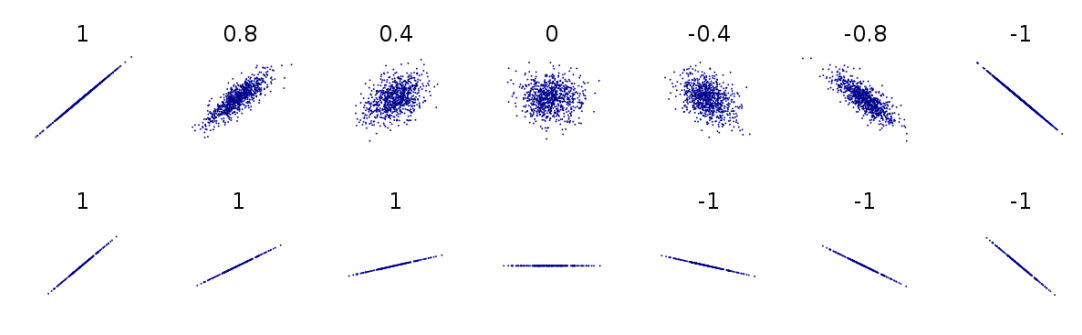
\includegraphics{images/largen/correlation.png}
\caption{Different correlations, visualized. The numbers represent correlation
coefficients. Based on Boigelot
(\protect\hyperlink{ref-boigelotdenisExampleCorrelationVarious2011}{2011}),
modified by Max Weylandt}
\end{figure}

Correlation coefficients can range from -1 to 1. Imagine that the different
graphs above represent the different possible relationships between education
(along the \(X\)-axis) and gender equality (on the \(Y\)-axis). As the top
line of figure 8.1 shows, a correlation coefficient closer to either pole
means a strong correlation while a number around 0 means a weak correlation.
If \(R=-0.8\), there is a strong negative correlation (at larger values of X,
Y tends to have lower values). If \(R=0.4\), there is a moderate positive
correlation (at larger values of X, Y tends to have higher values). The
correlation we got indicates that we have a fairly strong positive
correlation. In other words, countries with higher levels of education tend to
have higher gender equality overall.

But also note the difference between the two lines in the graph above. In the
bottom line, every image represents a perfect correlation, even though the
relationships between \(X\) and \(Y\) are clearly very different. On the first
graph from the left, \(Y\) increases a lot as \(X\) moves from its lowest to
its highest value. Two images over, \(Y\) still increases as \(X\) does, but
much less so. They both move in the same direction perfectly (they have a
correlation coefficient of \(R=1\)), but the slopes are different. This has
implications for our findings: is gender equality slightly higher in countries
with more education, or a lot higher? Correlation cannot answer that question.
Later, we'll see how regression accounts for this difference in slopes. By the
way, it is always a good idea to visualize your data. The graphs in the figure
below show three datasets that have almost identical means, medians, and
correlations - yet look quite different when plotted.

\begin{figure}
\centering
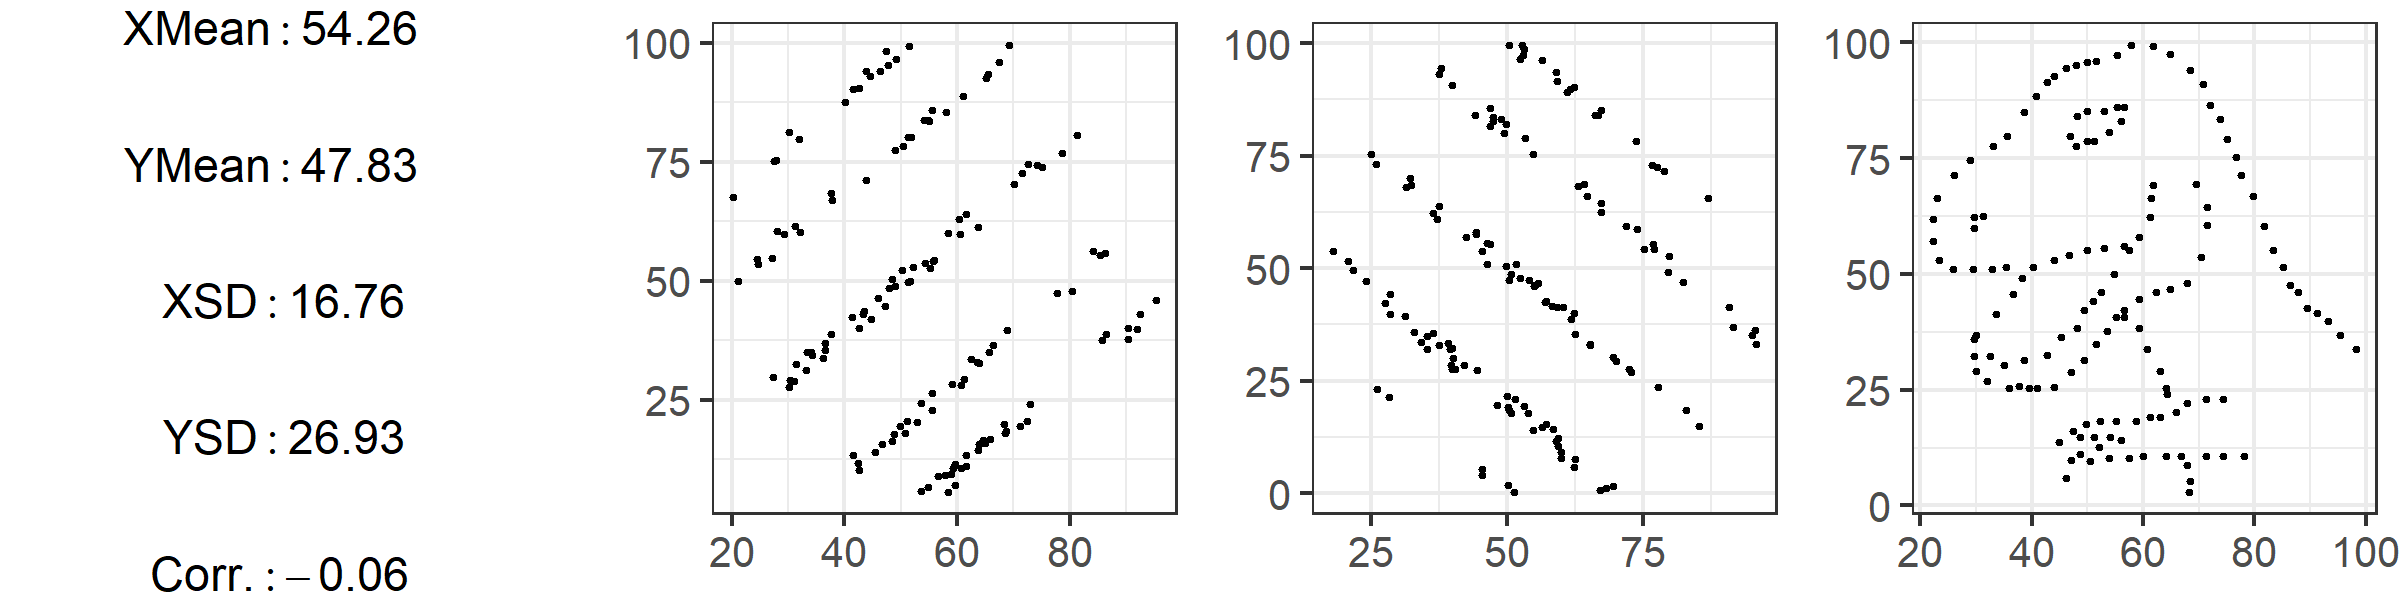
\includegraphics{images/largen/dino.png}
\caption{Based on the ``Datasaurus Dozen'' by Matejka and Fitzmaurice
(\protect\hyperlink{ref-matejkaSameStatsDifferent2017}{2017})}
\end{figure}

Correlations can easily be calculated with statistical software, and the
number of datasets available to researchers has exploded in recent years. This
means that, now more than ever, you can conduct exploratory analyses with a
large number of variables to see which ones are related to each other or the
outcome you are interested in. This process, of looking at large number of
variables and seeing how they relate, is sometimes called
\textbf{data-mining}. Data mining can be an acceptable part of an inductive
theory-building process (see ``Causal Inference and the Scientific Method''),
but it is a fraught process: when looking at a large number of variables you
are bound to find some that show a relationship, and it can be tempting (even
subconsciously) to write up only results that confirm our hypothesis rather
than those that don't.

\textbf{What does a correlation coefficient tell us? What does it *not* tell us?}

\begin{shaded*}

It tells us how strongly the variables in question are associated. It does not
tell us how large that association is. For example, variables can show a
perfect linear relationship, but we do not know if an increase in the first
variable is associated with a tiny or a large change in the second variable.

\end{shaded*}

\hypertarget{regression}{%
\subsection{Regression}\label{regression}}

Correlations are a useful first look at the relationship between two
variables, but linear regression is far more powerful. The intuition behind
linear regression is simple: we want to find the line that best fits all of
our data points. This is because the line that fits the data best summarizes
the relationship between variables, and we can use this line to learn not just
the direction of an association (positive or negative) but also its strength:
as \(X\) changes, \emph{how much} does \(Y\) tend to change? Regression also
lets us conduct significance tests to establish whether the relationship
between variables actually exists or just appears to occur due to chance.

\begin{figure}
\centering
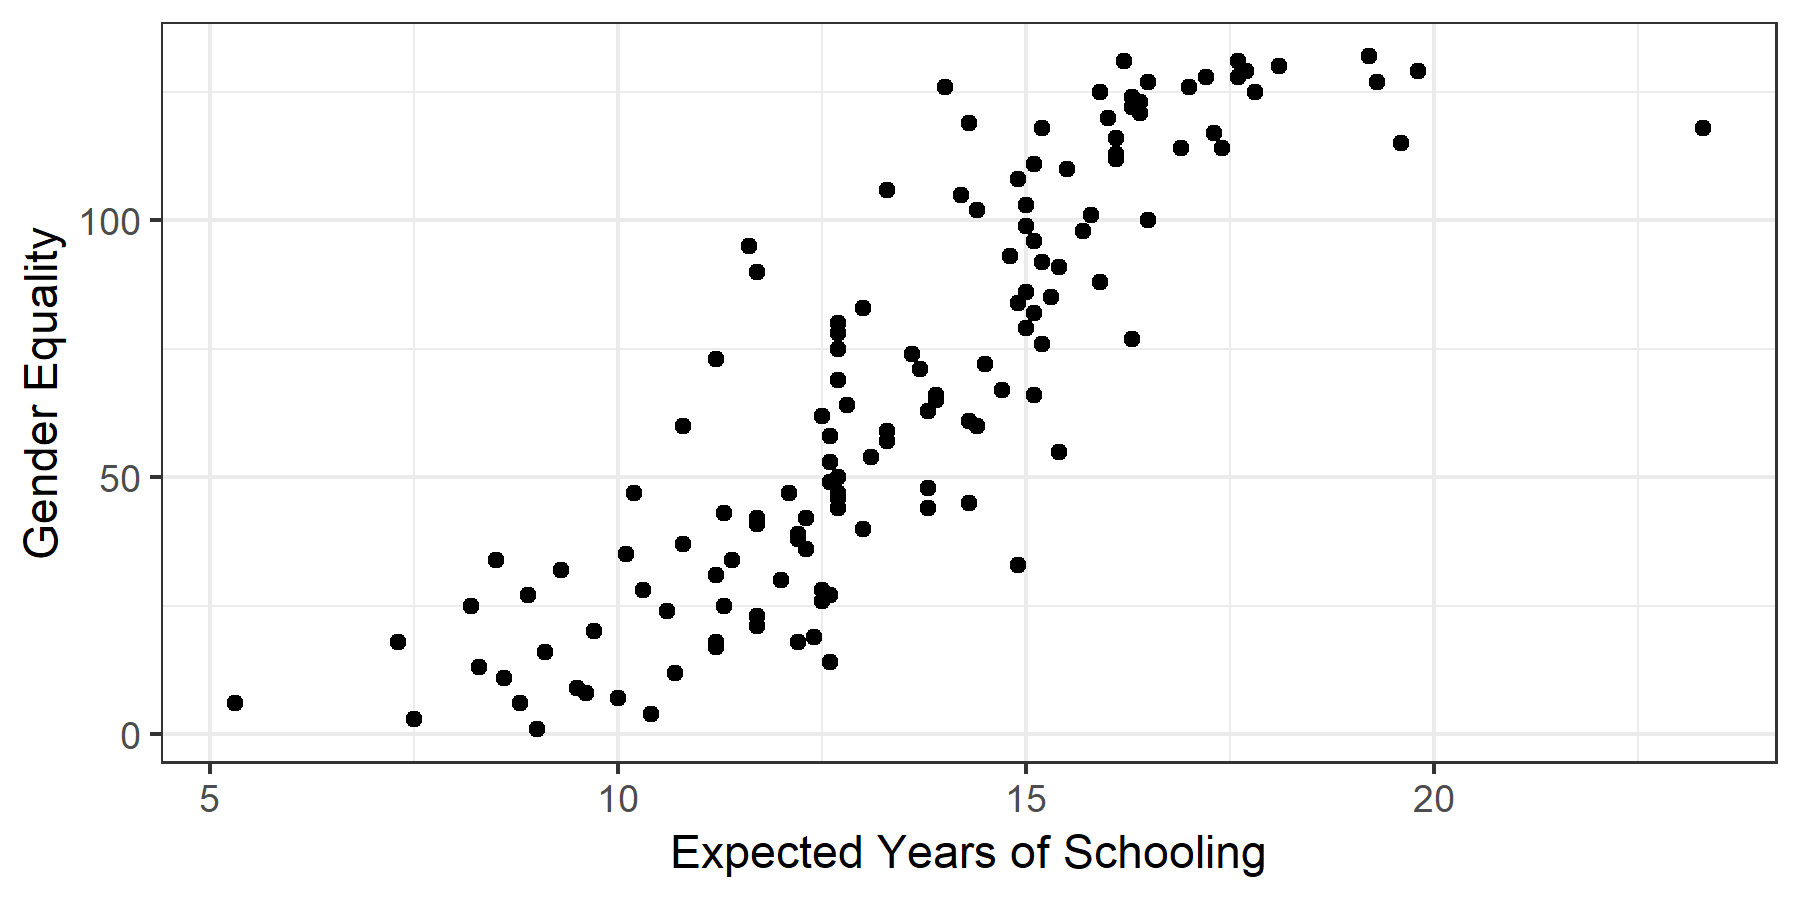
\includegraphics{images/largen/scatter.png}
\caption{A simple scatterplot}
\end{figure}

Perhaps it's best to start with an image. Figure ``A simple scatterplot''
charts the values for 147 countries' expected years of education against their
scores on the equality index, with each country represented by a dot. Just
from looking at it, you can see that countries with a high level of education
tend to have higher levels of overall gender equality, even if not all
countries neatly fit that description. In other words, as predicted by our
correlation coefficient of 0.85, it seems that there is a relationship between
education and gender equality. But how strong is this association?

To answer the question, we draw the line that best fits the data points in the
scatterplot. This straight line (this is \emph{linear} regression after all)
summarizes the relationship between the two variables we are interested in.
Imagine we wanted to explain the relationship to someone else but couldn't
show them the individual data points. We could still show them the line and
they would get a sense of how gender equality and education relate.

The regression equation takes the form: \[Y = a + bX\]

Take a second to appreciate what we have done here. We've taken data on two
variables for 147 countries, and summarized it with one line on the graph,
which we can in turn express as this simple formula. The formula may look
familiar to you, as it is simply the formula for a straight line. In the above
equation \(a\) is the intercept -- the value \(Y\) takes on when \(X=0\). In
other words, what is the level of gender inequality that a country with 0
years of expected schooling would have? \(b\) is the slope. Remember the
function the slope plays in a graphs: it gives you `rise over run', telling
you how much the \(Y\) tends changes in relation to the \(X\). This means that
in a regression equation, the slope is very important, because it expresses
the relationship between our variables: on average, a one-unit increase in the
X variable (in our case, one year of extra expected schooling) is associated
with a \(b\)-sized increase or decrease in the outcome variable (points on the
gender equality index). The slope \(b\) is often also called the
\textbf{regression coefficient}. In the case of our regression line,
\(b=11.6\). As you will see below, we often encounter regressions with
multiple variables, each of which has its own coefficient (i.e.~change in the
outcome variable associated with change in the independent/input variable).

In our example, the intercept \(a=-89.2\). This is a good time to warn you
about extrapolating using data from regression. That intercept is impossible,
because the way our outcome variable is set up, there are only positive scores
for equality. Yet because of the best fit line, our regression predicts an
impossible value for \(Y\) when \(X=0\). Always remember that regression fits
the line based on the data available. If you want to use it to make prediction
about data points far away from the data you actually have, it is possible the
prediction will be way off. (By the way, you can find the values for both
\(a\) and \(b\) in Table 8.1 below. We'll discuss how to interpret the table
in more detail below, but feel free to see how much you can get from it right
now).

\begin{figure}
\centering
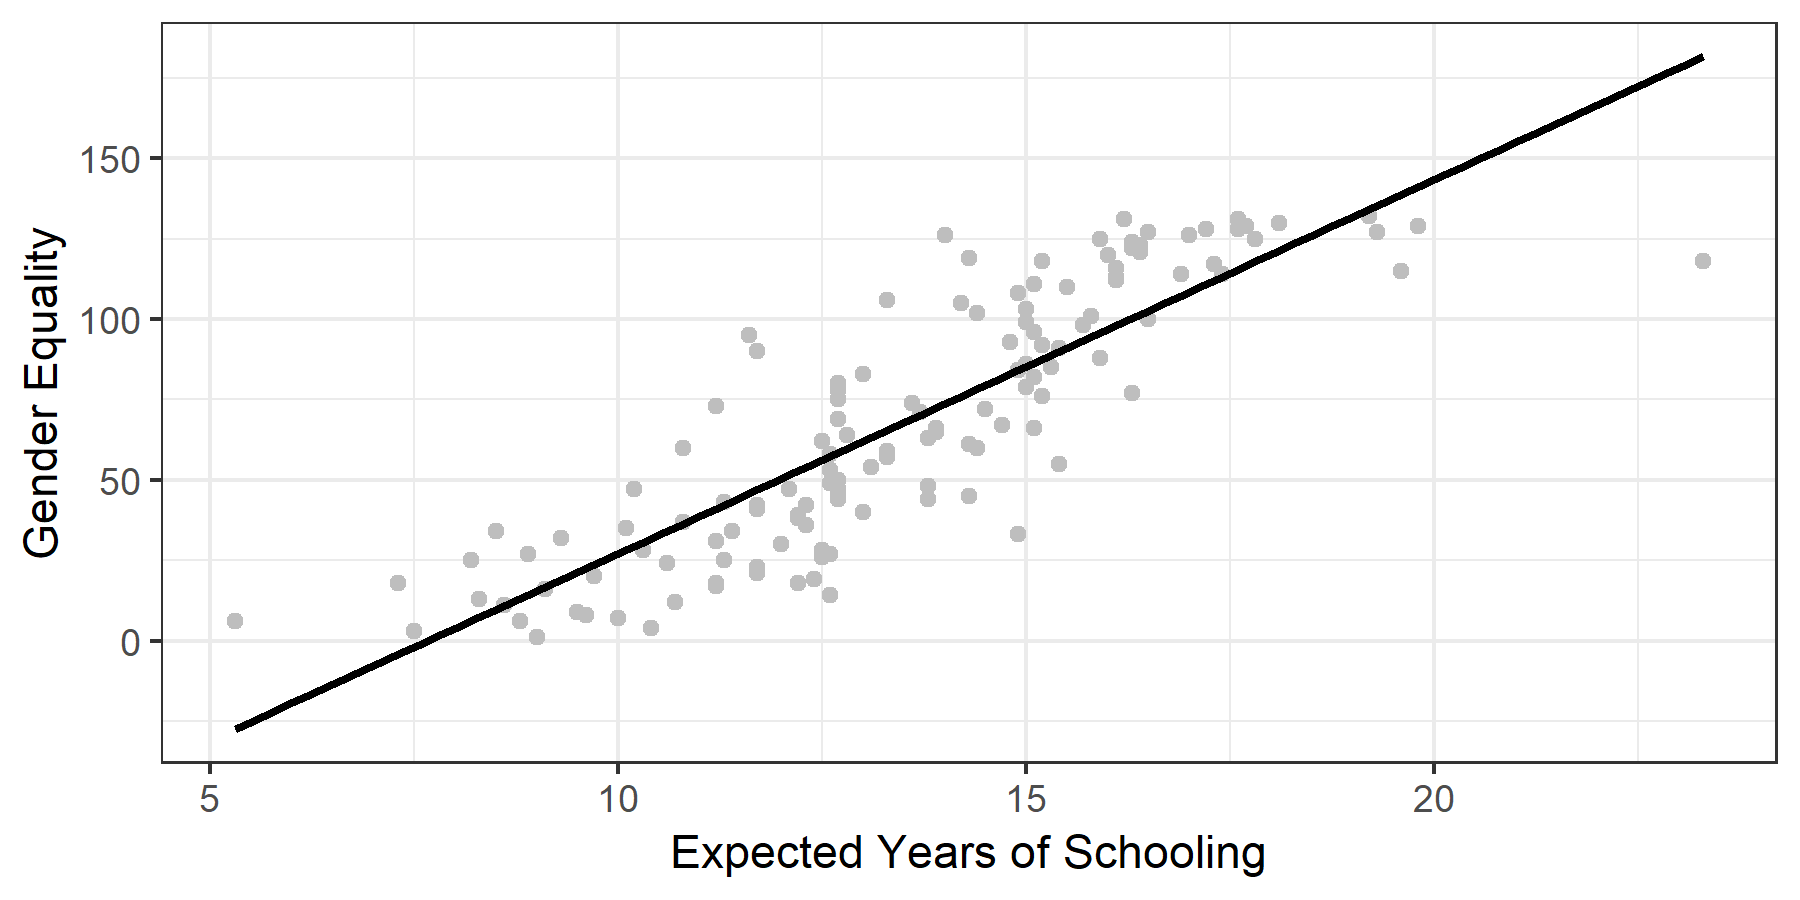
\includegraphics{images/largen/line.png}
\caption{The regression line}
\end{figure}

\hypertarget{method-detail}{%
\section{Method: detail}\label{method-detail}}

\hypertarget{finding-the-line-of-best-fit}{%
\subsection{Finding the Line of Best Fit}\label{finding-the-line-of-best-fit}}

How do we find the line that fits the data best? Let's restate our aim: we
want a line where, given a certain \(X\) value, the \(Y\) value predicted by
the line is really close to the actual value in the data. That seems like a
reasonable definition of `good fit.' Rephrased in mathematical terms, we want
to be as small as possible. The thing we want to minimize is called a
\textbf{residual}. For example, in ``The regression line'', Serbia has an
expected years of schooling value of \(14.6\) and a gender equality score of
\(106\). Those are the actual values in the dataset. However, the regression
line predicts that an education (i.e.~\(X\)) value of \(14.6\) is associated
with a gender inequality score of \(82.94\)
{[}{\(Y= a+ bX= -89.2 + 11.6 \cdot(14.6) = 80.16\)}{]}. The residual amounts
to \(25.4\) {[}{\(106 - 80.16=25.4\)}{]}, and is highlighted with a blue line
in ``Visualizing Residuals'' below.

\begin{figure}
\centering
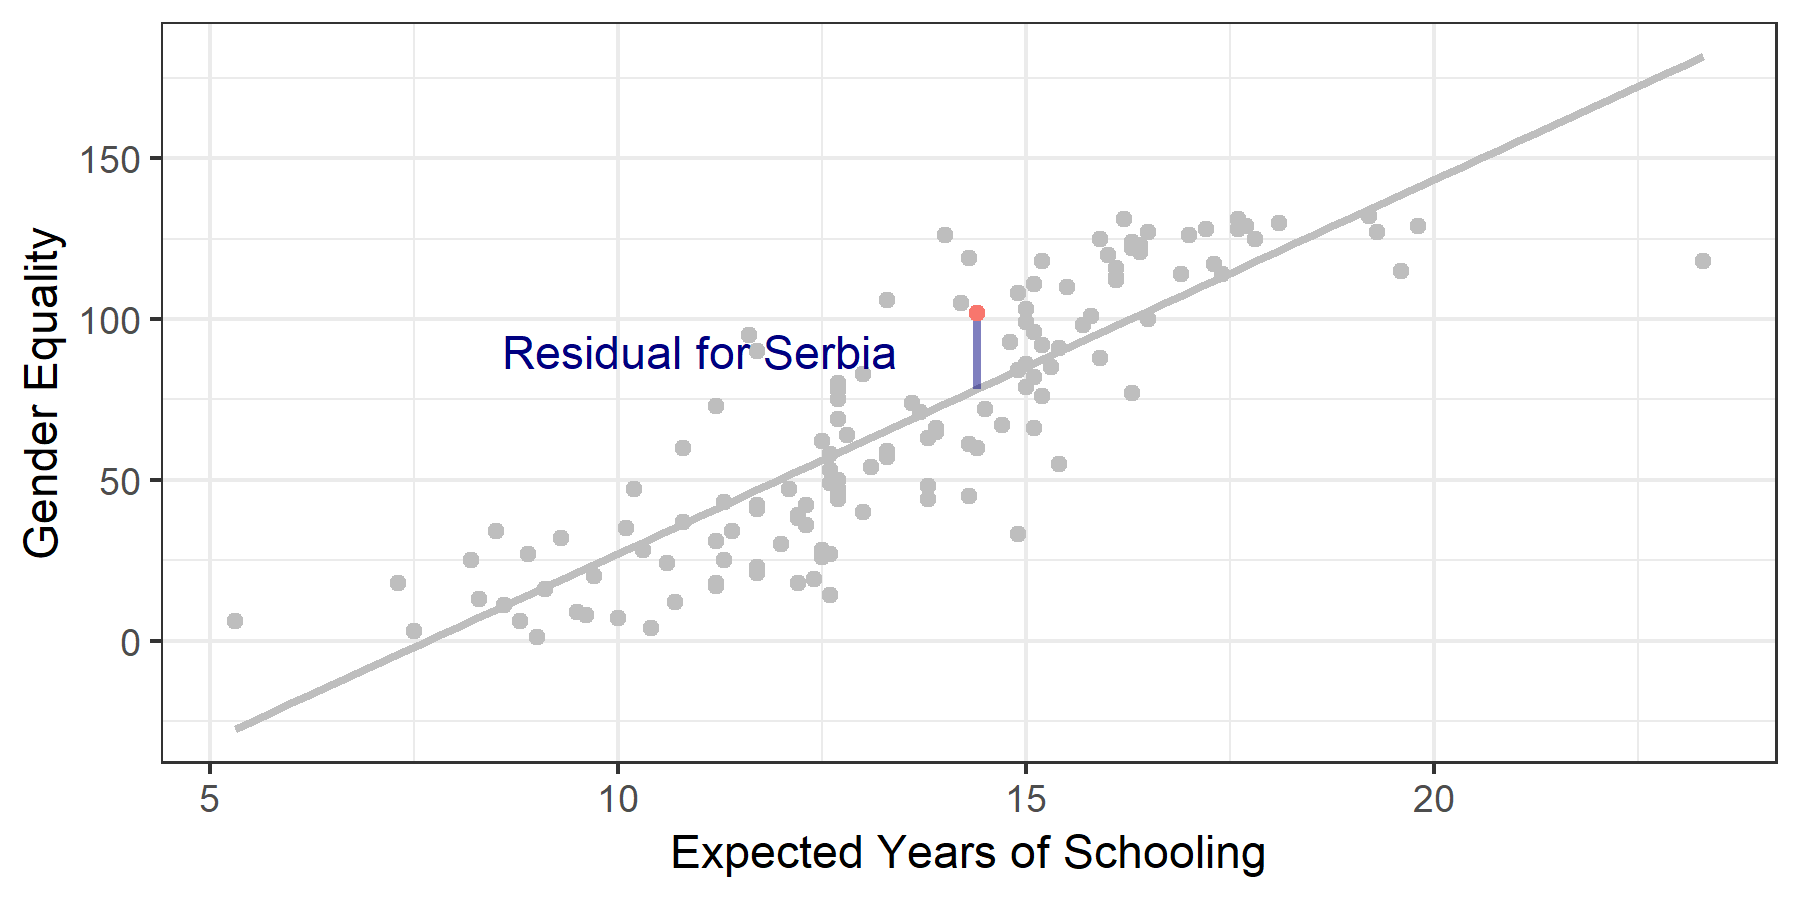
\includegraphics{images/largen/residuals.png}
\caption{Visualizing Residuals}
\end{figure}

We take a cumulative look at all of our residuals to see which line fits best.
There are several possible methods for doing this. Simply adding up the
residuals would give us misleading results: some are negative and some are
positive, and they would cancel each other out. To deal with this problem we
square each residual. This makes all values positive, and has the added
benefit of penalizing larger differences between our line and actual values.
We find the line that best fits our data by minimizing the squared residuals.
This procedure is called \textbf{ordinary least squares}.

The line you see in figure ``Visualizing Residuals'' is the line of best fit.
Still, as you can also see, there are residuals. This is because in linear
regression we are trying to find one single straight line to best predict the
data, which always results in some points being off the line. A line that hits
all points is possible but its equation would be so complicated it would be
impossible to interpret. The key is that any other line would have residuals
that are overall further away. The image below shows how different lines have
drastically different squared residuals. For an interactive example that lets
you adjust the line and see how the squared residuals change, check out the
second image on
\href{http://setosa.io/ev/ordinary-least-squares-regression/}{this page}.

As you can see, we can draw an infinite number of lines through our data, but
the one where the squared residuals are lowest is the line of best fit -- the
line that best describes the relationship between our variables X and Y.

\textbf{Why do we want to fit a line through our scatterplot?}

\begin{shaded*}

The line that best fits the data gives us a simplified, approximate summary of
the relationship between our variables.

\end{shaded*}

\hypertarget{significance-tests}{%
\subsection{Significance Tests}\label{significance-tests}}

Regression lets us test whether the relationship between our variables is
statistically significant. We begin by setting up a hypothesis test in the
format with which you are already familiar. Our null hypothesis is that the
relationship between variables \(X\) (education) and \(Y\) (gender equality)
--- AKA the coefficient \(b\) -- is zero.

\[H_0: b = 0\] \[H_a: b \neq 0\]

In our example, we find a beta that is not zero, \(11.6\) in the bivariate
regression we conducted. How weird is this? We can calculate how unlikely it
is to get \(11.6\), if \(b\) is actually 0 like our null hypothesis
stipulates. This calculation gives us a p-value for the coefficient. If the
p-value is lower than a threshold we set ahead of time, we call the
coefficient statistically significant. This just means that we have a high
degree of certainty that \(b\) really is not zero.

You can see the details of this calculation in the
\href{./mathematical-appendix.html}{Mathematical Appendix}.

Another way of approaching this issue is to calculate a 95\% confidence
interval for the coefficient -- a range for which we have 95\% certainty that
the coefficient falls within its confines. In our example, the 95\% confidence
interval for the coefficient \(b\), which captures the association between
education and gender equality, is \([10.4, 12.8]\). (You can see the
calculation in the ). If the entire range is positive (as it is for us) or
negative, it means that we are 95\% certain that the true coefficient is not
zero. The null hypothesis says that there is no relationship between \(X\) and
\(Y\). But our interval is so far away from zero that we can feel safe
rejecting the null hypothesis.

\hypertarget{multivariate-regression}{%
\subsection{Multivariate Regression}\label{multivariate-regression}}

As social scientists, the phenomena we investigate are usually very
complicated, and we seldom deal with bivariate relationships alone. In terms
of our above example, there are many factors other than education that could
affect gender equality. For example, what if wealth is the variable we are
looking for, not education? What if it's simply countries where people are
wealthier that have higher levels of gender equality?

A bad way of addressing this issue would be to simply run a second regression,
looking at the relationship between wealth and gender inequality, and then
compare the results. If we do this, we miss potential relationships between
all of our variables. (You may remember this discussion from ``Causal
Inference and the Scientific Method''). Maybe wealth brings more education and
also more gender equality, explaining why we think we see a relationship
between education and equality. If we are just looking at the effect of
education on equality, we are probably giving education credit for some of the
variation in equality that is due to wealth. Education's actual effect would
be lower. This is a general rule: When we leave out variables that affect our
main relationship, we tend to overestimate the regression coefficients of the
variables in our regression. This is called \textbf{omitted variable bias}:
leaving out relevant variables results in faulty (usually inflated) estimates.

Luckily, regression allows us to control for other variables. At this point it
becomes harder for us to rely on graphs: representing two variables on a graph
is easy, but once we add more we are dealing with too many dimensions to
represent on a screen (or grasp with a human brain, at some point!). What you
need to know is the following: we can remove the influence other variables
have on the outcome variable and look at the effect of only our variable of
interest. When you read a paper that talks about ``controlling for'' or
``keeping constant" other variables, this is what they are doing -- once we
have accounted for the variation in the outcome explained by `control
variables', what is the relationship between the variable we care about and
the outcome? The neat thing is that the output we get from running a multiple
regression doesn't just report on our main variable and the outcome, now
controlling for other factors. Instead, it gives us the association between
every single variable and the outcome, controlling for all the other variables
included in the calculation. Thus including several variables in one
regression is desirable for two reasons: first, because we simply want to know
the effect of several variables, and second, because leaving out relevant
variables would give us less accurate results.

A multiple regression with two explanatory variables can be written as:
\[Y = a + b_{1}X_{1} + b_{2}X_{2}\] Academic papers will often use \(\beta\)
instead of \(b\), \(\alpha\) instead of \(a\), and sometimes even write
variable names directly into the formula. In terms of our example we could
write: \[Ineq = a + \beta_{1}EDU + \beta_{2}GDP\]

Here, \(\alpha\) is the intercept (the value of gender equality we predict
when both education and GDP are at \(0\)), \(\beta_1\) tells us what change in
gender inequality is associated with a 1-unit increase in education, and
\(\beta_2\) tells us about the association between GDP and education.

\textbf{Why do we control for other variables?}

\begin{shaded*}

For two reasons. First, we might be interested in how other variables relate
to the outcome. Second, we want to hold constant the effect of other variables
to avoid omitted variables.

\end{shaded*}

\hypertarget{reading-a-regression-table}{%
\subsection{Reading a Regression Table}\label{reading-a-regression-table}}

When reading quantitative papers, chances are you will read a regression
table. Reading regression results is a key skill for engaging with political
science research. It will save you a lot of time, giving you results at a
glance, and help you critically compare the actual results of an analysis with
the findings the authors present.

Let's look at a regression table that shows the results of our analyses, Table
8.1. As you can see, each variable gets its own row -- often the main variable
of interest is in the top row. Also, each model gets its own column. Broadly,
a model is a different way of looking at the statistical relationship between
our variables. In our case, model just refers to different combinations of
variables. Other times, different models can feature more complicated
differences in statistical calculation. Column (1) shows the results of our
first model, which is the simple bivariate regression we began with. Here, in
the line for expected years of schooling, you can see the f the variable. You
interpret this as discussed above: a one-unit increase in the variable
(education) is associated with a 11.6 unit increase in the outcome variable
(gender equality). In other words, one extra year of expected schooling is
associated with an almost 12 point higher score on the gender equality index.

\begin{figure}
\centering
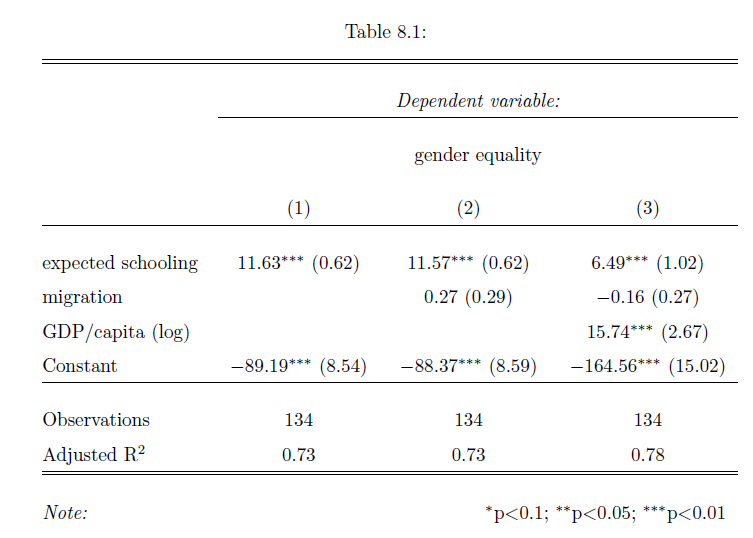
\includegraphics{images/largen/large-n-results-table.png}
\caption{Table: 8.1}
\end{figure}

The little asterisk next to the coefficient is a very common symbol to denote
statistical significance. A legend at the bottom of the table (as in our
example) will explain what different symbols mean, but the standard meanings
are shown in Table 8.1. You can see that education is statistically
significant at the 0.01 level - we are quite certain the coefficient is not
zero, and therefore quite confident that there is an association between
education and gender equality. Right next to the coefficient and the asterisks
is the standard error - our measure of uncertainty regarding our estimate of
the coefficient.

Column (2) shows the results of a second model where we also add the net
migration of a country. We can also read the association with this variable
from the table: the ndicates that a 1-unit increase in the migration index
results in a 0.27 increase in the gender equality index \emph{holding all
other variables constant}, but the finding is not statistically significant.

In Column (3) we add GDP/capita to account for different levels of wealth, and
you can see that the s substantially lower than in the previous two models.
The table indicates that a one-unit increase in education is now associated
with a 6.5 point increase in gender equality, \emph{holding all other
variables constant}. This change in coefficient illustrates the problem of
omitted variable bias. Before we explicitly looked at the relationship between
wealth and gender inequality, we were giving education too much credit. It
seems that GDP explains some of the variation in gender equality that we had
previously attributed to schooling. Indeed the s sizable and statistically
significant.

\begin{figure}
\centering
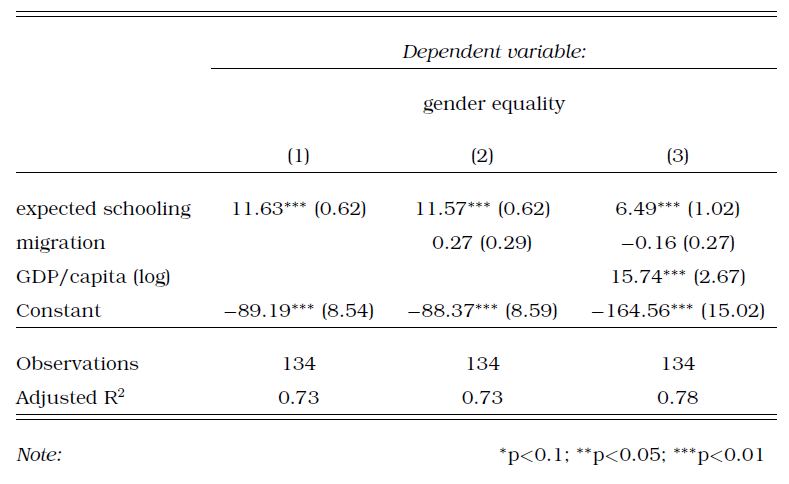
\includegraphics{images/largen/table8.2.png}
\caption{Table: 8.2}
\end{figure}

The coefficient of our main variable of interest - education - changes a fair
amount when we change the model. When an association remains despite us
changing the models around, we say that it is \textbf{robust}. If our variable
remains significant across different models, it gives us more confidence that
the association is actually there. If introducing control variables means that
the main interest is not significant, we would question whether our
association is actually there or not. There is no hard and fast rule for
judging robustness. In our case, controlling for GDP did mean that the effect
size of education went down by quite a lot. This is somewhat worrying. On the
other hand, education did retain a statistically significant association
throughout.

You'll note that the variable is called GDP/capita (log). This reflects a
common practice when dealing with GDP, which is to convert the values first
before using them in the regression. This is statistically sound, but makes
interpretation more difficult -- see the for more details if you are
interested.

The final line among our variables, \emph{Constant}, denotes the intercept.
Sometimes this is at the bottom, sometimes at the top of the table. We already
discussed how to interpret this: if all \(X=0\), the regression line predicts
that \(Y\) will equal the value of the intercept.

Let's move further down the table. The \(\mathbf{R^2}\) tells us how much of
the variation in Y is explained by our regression line. The regression line
above (model 1 in the table) has an \(R^2\) value of 0.73. This is also
referred to as ``goodness of fit" (i.e.~how well does the data fit the line?).
This \(R^2\) indicates that our regression line accounts for \(73\%\) of the
variation in gender equality.

It is tempting to simply scan the table to see which variables have stars
associated with them, and conclude only they matter because they have
statistical significance. But statistical significance is not everything. We
also have to consider \textbf{substantive significance}, which is linked to
the size of the coefficients. If a regression shows that a variable is
significant at the .01 level, but it has a tiny coefficient, what does it
mean? It means the variable may well be associated with a change in the
outcome variable, but that this change is tiny. As social scientists, we are
studying real-life phenomena and so we should care about the substantive
impact of different variables on our outcome. We want to see effects that are
perceptible in real life, not just in the data! On a practical note, however,
do not be surprised at small effect sizes. The phenomena we study are complex
and so it often makes sense that any given factor only has a small effect. As
research methods have improved over the last decades, we have seen a decrease
in effect sizes which suggests some older research suffers from omitted
variable bias (remember that term?)

In short, here's how to read a regression table:

\begin{enumerate}
\def\labelenumi{\arabic{enumi}.}
\item
  Begin with the first column and read it top to bottom. Note variables'
  coefficient sizes and whether they are statistically significant.
\item
  Move to the next column and do the same. See which coefficients change and
  in what direction. Which coefficients are no longer significant once other
  controls are added or the model changes in other ways?
\item
  Track the main explanatory variable across models. Is it robust to the
  inclusion of controls and across different model specifications?
\item
  Compare your impressions with the descriptions of the authors. Do they
  discuss all relevant findings, or do they leave something out?
\end{enumerate}

In recent years, more authors have begun to display regression results in a
graphical way. Consider figure 8.6 below, which displays the result of Dionne
and Horowitz's 2016 article
(\protect\hyperlink{ref-dionnePoliticalEffectsAgricultural2016}{Dionne and
Horowitz 2016}). Their regression estimates the probability of farmers
receiving agricultural subsidies. The dots represent the coefficient estimates
from their regression, and the horizontal whiskers show the 95\% confidence
interval. At a glance, you can see that two confidence intervals do not
contain 0, meaning we are 95\% sure that the real value of these coefficients
is not 0 -- they are statistically significant. We also see that their value
is negative, meaning that households with a female head and those that had
seen death or illness were less likely to receive aid.

This figure also shows an example an example of something you should know
called a \textbf{dummy variable}. The term `dummy' bears no relation to what
these variables do: they only take two values (yes or no, 1 or 0) and can be
used to compare groups. When we include a dummy variable in a regression, the
output tells us the difference in average Y values across the two groups. In
this example, females receive aid at lower rates than males (the two values of
these dummy variables). If you look at the variables in figure 8.6 you will
see that many of them are dummies: they denote membership in ethnic groups,
partisanship, and more. Rather than interpreting the coefficient as "a one
unit increase in X is associated with a \(b\) increase in Y," we think "being
X rather than not is associated with a \(b\) increase in Y."

\begin{figure}
\hypertarget{fig:dotwhisker}{%
\centering
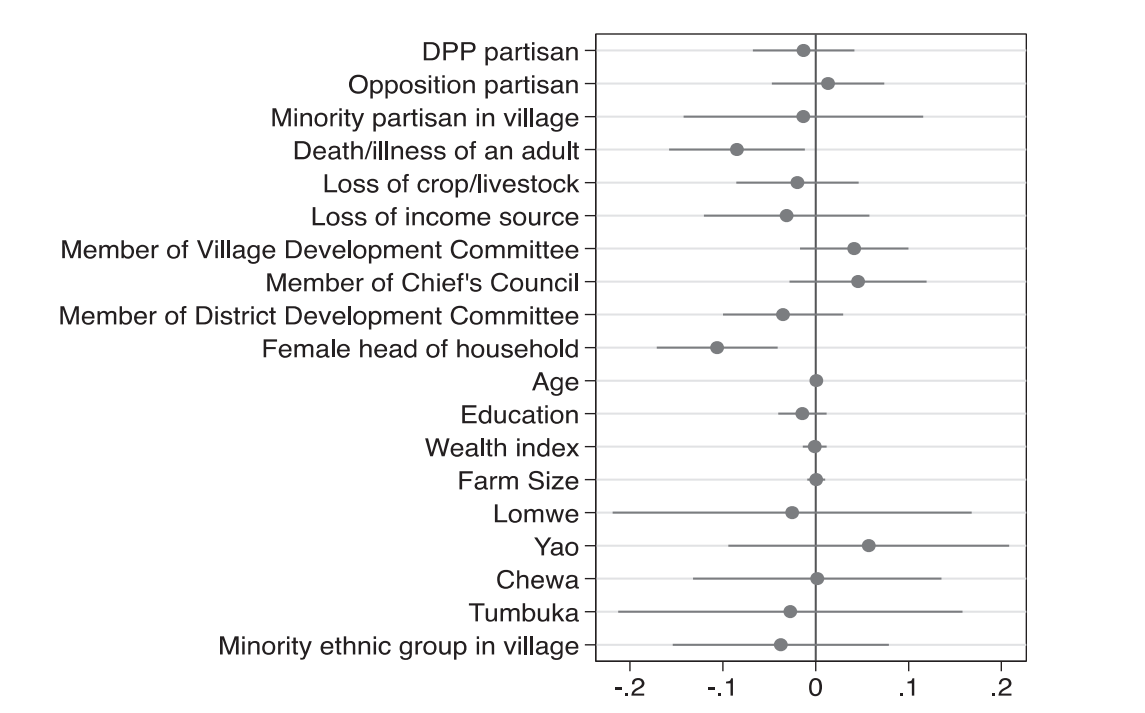
\includegraphics{images/largen/dotwhisker.png}
\caption{Adapted from Dionne and Horowitz 2016, 220}\label{fig:dotwhisker}
}
\end{figure}

\hypertarget{applications-2}{%
\section{Applications}\label{applications-2}}

\hypertarget{correlation-1}{%
\subsection{Correlation}\label{correlation-1}}

Simple correlations are not as often found in recent scholarship as
regression, mostly because regression is far more powerful and flexible than
correlation, and hardly more difficult to calculate. Still, as noted above,
correlations can be useful for an initial look at the data and when describing
data. Take Whitaker and Lynch
(\protect\hyperlink{ref-whitaker2011explaining}{2011}), who are trying to
understand the success of the UK Independence Party at the 2009 European
Parliament Election. The first thing they do is simply to see whether support
for UKIP correlates with support for the conservative or labour parties in the
same geographical area, before moving on to a more sophisticated regression
that relates support for UKIP to a number of demographic factors.

You will also encounter correlations in more technical sections of papers,
when authors discuss which variables to use to measure certain concepts. For
example, there are several different measures of democracy: Polity, the V-Dem
Institute, and Freedom House all offer datasets that score each country's
level of democracy for a given year. In papers using democracy as a variable
(be it outcome or explanatory), authors often pick one of them rather than
running the analysis several times. They might note, however, that the indices
are highly correlated -- suggesting that results would be similar regardless
of the dataset chosen. Below, we will look at a study by Kuenzi amd Lambright
where the outcome is level of democracy. They write:

\begin{quote}
...the polity scores for these 33 cases are highly correlated with the other
measures of democracy. For example, the polity scores are also highly
correlated with the Freedom House total scores for 2000 (r = --0.88; higher
values on the Freedom House measure correspond to a lower level of democracy).
(\protect\hyperlink{ref-kuenziPartySystemsDemocratic2005}{Kuenzi and Lambright
2005, 428})
\end{quote}

\hypertarget{regression-1}{%
\subsection{Regression}\label{regression-1}}

We are talking about large-N data in this chapter, and regression is most
useful when applied to a fairly large number of cases. Some of this research
takes data from different geographical or political units to look at a
phenomenon across many cases, like the example about education and gender
equality earlier on in this chapter.

\begin{figure}
\centering
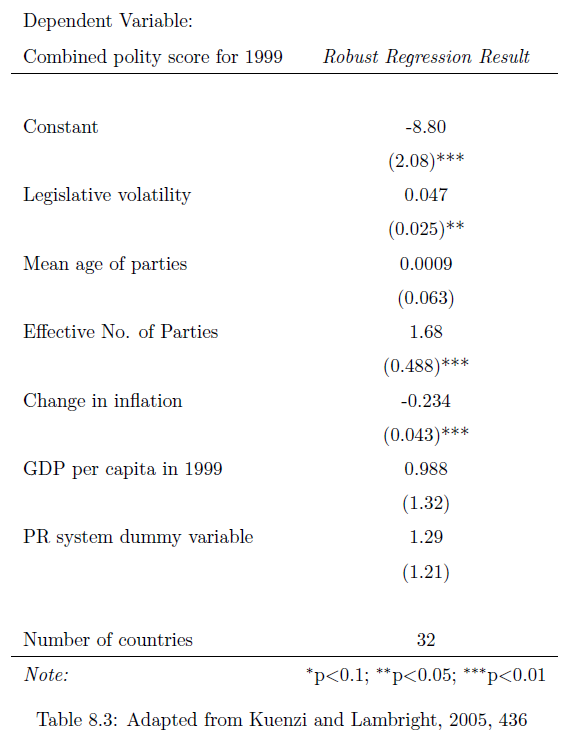
\includegraphics{images/largen/table8.3.png}
\caption{Table 8.3}
\end{figure}

Kuenzi and Lambright want to look at the relationship between party systems
and the level of democracy along a number of African countries. Their outcome
is a country's score on the Polity scale, and their variables of interest are
legislative volatility, the effective number of parliamentary parties, and the
average age of parties
(\protect\hyperlink{ref-kuenziPartySystemsDemocratic2005}{Kuenzi and Lambright
2005}).

Look at Table 8.3 to get a sense of the results. Let's interpret these
coefficients. We can see that a one-unit increase in legislative volatility is
associated with 0.047 more points on the polity index, holding all other
variables constant. This is significant at the 0.05 level.

\textbf{Interpret the coefficient for the effective number of parties. What does the coefficient tell us?}

\begin{shaded*}

Looking across countries with different party systems, one additional
effective party is associated with a 1.68 point increase on the polity score,
controlling for the other variables in the regression.

\end{shaded*}

\hypertarget{logistic-regression}{%
\subsection{Logistic Regression}\label{logistic-regression}}

Logistic regression is a type of regression where the outcome variable, \(Y\)
can only take on two values, 1 or 0. (Our discussion about dummies earlier was
focused on explanatory (\(X\)) variables).

This is what Garcia (2006)
(\protect\hyperlink{ref-garcia-riveroRaceClassUnderlying2006}{García-Rivero,
n.d.}) does, studying respondents' feelings about the ruling party in South
Africa, the ANC. The outcome variable is whether or not voters felt close to
the ANC (1) or did not feel close to it (0). He looks at several demographic
indicators to see which factors are associated with support for the ANC. You
will find a lot of logistic regressions of this type in the study of
elections, where voting intention is often a categorical variable.

Logistic regressions are slightly more tricky to interpret than regular
regressions. To illustrate, let's look at the main table from Ferree (2006)
(\protect\hyperlink{ref-ferreeExplainingSouthAfrica2006}{Ferree 2006}), who
wants to understand why South Africa's election results seem to have split
along racial lines. The outcome variable is whether voters intended to vote
for the ANC (1) or did not plan to vote for it (0). She looks at several
exploratory variables, as you can see in Table 8.4.

\begin{longtable}[]{@{}lc@{}}
\toprule
& Support for the ANC \\
\midrule
\endhead
Performance rating & 0.817 \\
& (0.431) \\
Believe DP is exclusive & -.196 \\
& (0.611) \\
Believe NNP is exclusive & 3.719** \\
& (0.604) \\
ANC partisan & 3.026** \\
& (0.582) \\
Female respondent & -1.454** \\
& (0.547) \\
Age & 0.040 \\
& (0.126) \\
Low schooling (no high school) & 0.998 \\
& (1.016) \\
High schooling (post matric) & -4.400** \\
& (0.713) \\
Political interest & .530** \\
& (0.251) \\
Pseudo R2 & .85 \\
N & 810 \\
\bottomrule
\end{longtable}

In the second column of Table 8.4, the coefficient for the variable `High
schooling' is -4.4. How do we interpret this? Clearly, we cannot do as we did
above: we can't say that having high schooling is associated with a 4.4 unit
decrease in the intention to vote for the ANC, because the only possible
values are either 0 or 1.

Instead we can do an anti-log on the coefficients to get odds ratios. What are
odds ratios? If the odds of something happening are 50-50, the odds ratio is
\(\frac{50}{50}=1\), if they are 80-20, the ratio is \(\frac{80}{20}=4\).
These ratios are hard to interpret. We can convert them to probabilities, but
these ratios change depending on the value of \(X\). While the interpretation
is tricky, know the basic intuition: the coefficients tell us whether the
variable is associated with a higher (or lower) likelihood of observing the
outcome.

\begin{figure}
\hypertarget{fig:trippkang}{%
\centering
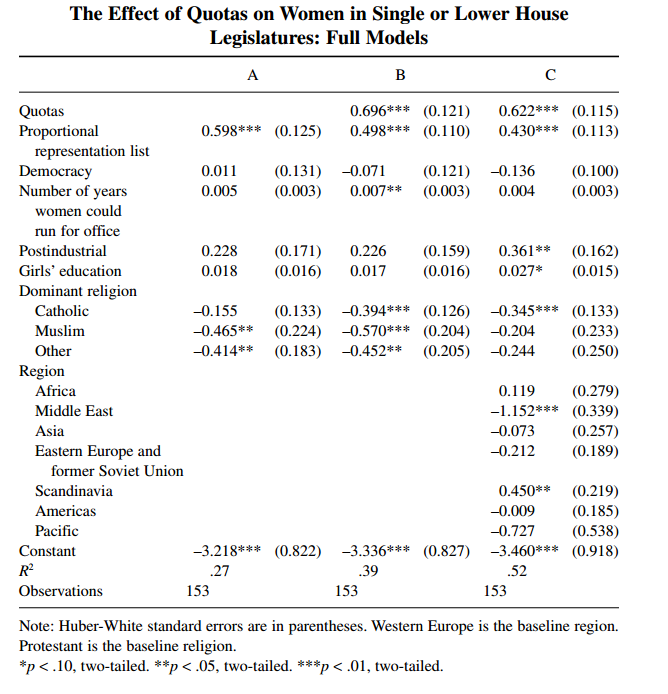
\includegraphics{images/largen/trippkang.png}
\caption{Adapted from Tripp and Kang 2008, 350}\label{fig:trippkang}
}
\end{figure}

\hypertarget{experiments-1}{%
\subsection{Experiments}\label{experiments-1}}

\begin{figure}
\hypertarget{fig:mengel}{%
\centering
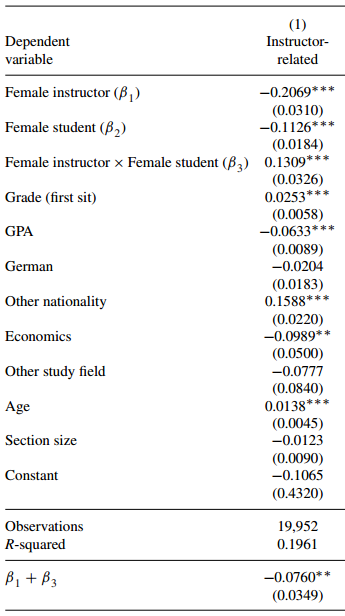
\includegraphics{images/largen/mengel.png}
\caption{Adapted from Tripp and Kang 2008, 350}\label{fig:mengel}
}
\end{figure}

You will also likely encounter papers using experiments or quasi-experiments,
which also use regression. As we discussed above, we can use dummy variables
to compare means across groups. In experiments, this means we can use
regressions to see how the treatment affected the treatment and control groups
in the experiment, but also how the effects differ for different demographic
groups, which we can add as control variables.

For example, Mengel, Sauermann, and Zölitz
(\protect\hyperlink{ref-mengelGenderBiasTeaching2019}{2019}) study how gender
affects teaching evaluations. There are by now
\href{http://www.rebeccakreitzer.com/summaries-of-research-articles/}{more
than 70 studies} indicating that women and people of color receive lower
teaching evaluations than their colleagues, all else equal. Mengel et al.~use
a `quasi-experiment': they look at data from courses where students were
randomly assigned to sections that could be taught by women or men. They write
that ``female faculty receive systematically lower teaching evaluations than
their male colleagues despite the fact that neither students' current or
future grades nor their study hours are affected by the gender of the
instructor" (\protect\hyperlink{ref-mengelGenderBiasTeaching2019}{Mengel,
Sauermann, and Zölitz 2019, 536}) The regression table to your right provides
more detail on controls: economics students, for example, tend to give lower
evaluations than students in other fields, and students with high grades in
the class tended to give higher scores. Overall, female instructors received
lower scores, as indicated by the negative coefficient on the explanatory
variable.

\hypertarget{advantages-of-method-2}{%
\subsection{Advantages of Method}\label{advantages-of-method-2}}

Regression is flexible, relatively easy to conduct, and intuitive. It enjoys
many advantages:

\begin{itemize}
\item
  \emph{Results are generalizable.} If the analysis is done carefully, we
  might be able to claim that the results we get from our analysis apply in
  other contexts too.
\item
  \emph{Regression gives precise results}. A regression output will give
  effect sizes, so not only do we know that one variable is associated with
  another, but also how large that association is. We can also construct
  confidence intervals for our estimates, giving us a sense of how certain we
  can be about the results.
\item
  \emph{Regressions make it easy to control for other variables}. We almost
  never deal with only bivariate relationships. Regression allows us to hold
  other variables constant while looking at the relationship we care about,
  minimizing our fear of omitted variable bias.
\item
  \emph{Regression allows for iteration}. Because of the relative ease of use
  of regression, other researchers can easily replicate research -- and build
  on it.
\end{itemize}

\hypertarget{limitations-of-method}{%
\subsection{Limitations of Method}\label{limitations-of-method}}

\begin{itemize}
\item
  \emph{Measurement}. One big problem of large-n quantitative research is that
  we can only compute statistics for variables we can measure. There are many
  things that have no measures (for example political will). On issues where
  we have measures, they are often controversial. For example, many scholars
  have tried to come up with databases that rate each country on a scale of
  democracy. But, as you have learned in the chapter on \emph{Data}, coming up
  with a single measurement for concepts is extremely complicated and always
  involves trade-offs. What is a democracy in the first place? Which aspects
  of a society should we consider? How should they be weighed? Many subjective
  decisions have to be made, all of which can greatly affect the measure given
  -- and therefore statistical results when entered into an analysis.
\item
  \emph{Average effects}. Regression is useful because it gives us a handy,
  simple output: for each variable it gives us a single coefficient that
  describes how much changing this variable affects the \(Y\)-variable.
  However, this is the average effect across all data points in our
  calculation. Look again at graph \protect\hyperlink{fig:scatter}{1}. The
  line, which gives us the regression coefficient, describes the data quite
  well (remember, we chose it because it is the straight line that does the
  best job of fitting the data!). Still, we can see that for some countries
  the line does a much better job at predicting the actual values than for
  other countries. In other words, \emph{on average} an increase of one unit
  in education is associated with a \(b\) increase in gender equality. But we
  should not conclude that this sort of relationship would hold for any one
  country we look at.
\item
  \emph{Bad application 1: unrealistic claims of causal inference.} The
  downsides of regression come often not from the method itself, but from how
  it has been used. Ironically, its ease of use has led to a large number of
  bad studies, because the ability to control for other variables has led
  scientists to feel a false sense of security. In reality, we often cannot
  control for all variables, either because we cannot measure them, or because
  it is difficult to think of all factors that might affect our outcome
  variable.

  There are many examples of authors claiming a multiple regression shows a
  causal relationship, using language about ``the effect of" one variable on
  another, and so on. These claims are often unrealistic. As you learned
  in''Causal Inference and the Scientific Method'', it is difficult to show
  causality. To show causality, we need to deal with endogeneity, including
  reverse causality (does Y cause X?) and omitted variable bias (is a third
  variable Z responsible for the relationship between X and Y we see in the
  data?). Another thing that can help is evidence for a mechanism through
  which X might affect Y. In the absence of such evidence, regression cannot
  show that one variable causes another.
\item
  \emph{Bad application 2: kitchen sink regressions.} Another thing
  researchers can do is to investigate a large number of variables until they
  find some relationship that either confirms their preferred hypothesis, or
  is at least interesting enough to warrant publication. This is similar to
  the practice of datamining discussed above, and is sometimes also called
  `p-hacking.' In fact, it is what I did to make figures 2-4 above: I was
  interested in a clear chart and regression table, and looked at different
  variables until I found a combination of variables that worked. With large
  datasets containing many variables so easily accessible, conducting a number
  of different regressions is dangerously simple.
\end{itemize}

\hypertarget{broader-significance-in-political-science}{%
\section{Broader significance in political
science}\label{broader-significance-in-political-science}}

Regression is perhaps the most commonly used quantitative technique in
political science. You've seen that the basic regression is very flexible and
gives us important information -- the strength of association between one
variable and another, even holding other factors constant. This is very
powerful! You've also seen one variation of it, logistic regression, but there
are many more extensions of the basic concept for a variety of applications.
Regression is used to analyze survey data, compare trends across place and
time, and to interpret the results of experiments. If you will conduct
research using large-N quantitative data, chances are you'll use linear
regression (or a method based on it). If you read research based on large-N
quantitative data, chances are you'll be reading a regression table.
Hopefully, this chapter got you closer to being able to do so.

\hypertarget{application-questions-6}{%
\section{Application Questions}\label{application-questions-6}}

\textbf{Explain the meaning of the coefficients \$a\$ and \$b\$ in the bivariate regression equation.}

\begin{shaded*}

\(a\) tells us the predicted value of \(Y\) when all of the \(X\)-values are
set to 0. On the scatterplot which visualizes the bivariate relationship, it
is the intercept.

\(b\) summarizes the relationship between \(X\) and \(Y\). It tells us how
much of a change in \(Y\) is associated with a 1-unit change in \(X\).

\end{shaded*}

\textbf{You collect data on two variables and get the computer to calculate a regression equation for you. To check it, you plug an X-value from the dataset into your equation. The Y-value that results from this calculation is different from the Y-value in the dataset. Is it a problem if the regression's predicted values differ from the actual values in the data?}

\begin{shaded*}

No.~In linear regression we are trying to fit a straight line through a large
number of data points. This means that one line will never perfectly fit all
points. It's fine if there is some difference - the importance is that we keep
those differences (residuals) as small as possible, in a process we call
ordinary least squares.

\end{shaded*}

\hypertarget{key-terms-5}{%
\section{Key Terms}\label{key-terms-5}}

\begin{itemize}
\item
  bivariate regression
\item
  data mining
\item
  logistic regression
\item
  multiple regression
\item
  omitted variable bias
\item
  regression coefficient
\item
  reverse causality
\item
  robust
\item
  statistically significant relationship
\end{itemize}

\hypertarget{small-n}{%
\chapter{Small N}\label{small-n}}

\textbf{By Justin Zimmerman}

\hypertarget{introduction-7}{%
\section{Introduction}\label{introduction-7}}

The field of political science has traditionally focused on the importance of
hypothesis testing, causal inference, experiments and the use of large n data.
Quantitative methods in all its capacities is without a doubt important, but
what can be lost at times is the value of small n methods of inquiry within
the field of political science. Researchers such as Kathy Kramer, Cathy Cohen,
Reuel Rogers, and Jennifer Hochschild et. al.~have all used small n methods to
tell stories about particular groups that have rarely been highlighted in
political science. Whether its identifying rural consciousness in Wisconsin
(\protect\hyperlink{ref-kramer2016a}{Kramer 2016}), researching the secondary
marginalization of the most disfranchised in the black community
(\protect\hyperlink{ref-cohen1999a}{Cohen 1999}), explaining the unique
political stances of Afro-Caribbean immigrants
(\protect\hyperlink{ref-rogers2006a}{Rogers 2006}), or highlighting the
politics of a new racial order
(\protect\hyperlink{ref-hochschild2012a}{Hochschild, Weaver, and Burch 2012}),
small n data can allow for a researcher to discover new information not easily
attainable through quantitative methods alone. Small n methods allow for a
more in depth assessment of a particular area and people.

This chapter will focus on the importance small n research. The chapter will
highlight the various methods for conducting small n research including:
interviews, participant observation, focus groups, and process tracing, as
well as the various procedures for determining case selection. First, the
chapter will elaborate the differences and goals of small n research as
compare to quantitative research.

\hypertarget{background-2}{%
\section{Background}\label{background-2}}

To be a well-rounded political scientist it is important to understand that
not every question can be answered through quantitative methods alone. There
are times when small n methods are the more appropriate option. Yet, how does
a researcher decide when small n methods are appropriate for their research?
The researcher must be able to identify the differences and purposes of small
n qualitative research and quantitative research. First, quantitative research
focuses on the effects of causes, while qualitative methods is focused on the
causes of effects. In other words, quantitative research, especially with
regards to causal inference, aims to figure out if a particular treatment
causes a particular outcome, such as an increase in an individual's education
causes them to be more political mobilized.

Small n qualitative research on the other hand focuses on understanding how
the outcome came to be. American Political Development (APD) scholars are a
great reference to this line of thinking. APD scholars look to track why
certain outcomes came to be, such as Paul Frymer's work on Western expansion
in the United States of America (\protect\hyperlink{ref-frymer2017a}{Frymer
2017}) or Chloe Thurston's research on housing policy and how it has
historically discriminated against women, African Americans, and the poor
through the use of public-private partnerships
(\protect\hyperlink{ref-thurston2018a}{Thurston 2018}). Small n qualitative
research also includes oral histories such as those provided by Yolande Bouka
concerning the Rwandan genocide (\protect\hyperlink{ref-bouka2013a}{Bouka
2013}) and the interviews and historical context to explain the coercive power
of policing in Latin America as researched by Yanilda María González
(\protect\hyperlink{ref-gonz2017a}{González 2017}). In short, small n
qualitative research aims to tell a story of how an event or policy came to
be, and what are the experiences of particular groups because of a particular
event or policy.

Thus, a small n qualitative researcher must take care to ensure their work is
able to satisfy three characteristics of good qualitative research. First,
their research must emphasize the cause and the implications it has. Second,
good small n qualitative theories must explain the outcome in all the cases
within the population. Lastly, qualitative questions must answer whether
events were necessary or sufficient for an outcome to occur, with the cause
providing the explanation. To setup qualitative research it is important to
that understand that qualitative methods are interested more in the mechanisms
behind things. Small n approaches can help us explore the underlying process
such as how institutions evolve and change by gathering data about
institutions, but it can also be answered through looking at institutional
change in one or two contexts. Small n qualitative research can be inductive
as a researcher builds the theory and hypotheses from the data, or deductive
by testing theories and hypotheses with the data. What is critical in building
qualitative research whether inductively or deductively is case selection.

\hypertarget{case-selection}{%
\section{Case Selection}\label{case-selection}}

Case selection for small n qualitative research setup to use a small number of
cases in order to go into a deep dive into a specific subject. For instance, a
researcher may use a specific neighborhood to explain a specific political
characteristic of the community. Reuel Rogers conducts this exact research
when he interviewed Afro-Caribbean residents in New York City about their
political preferences as new immigrants of the United States of America
(2006). This case selection allowed for Rogers to assess the veracity of an
age old claim that pluralism allows for immigrants to eventually assimilate
into American culture and government participation by highlighting the
complexity that comes from immigrants that are identified as black. Rogers
finds that Afro-Caribbean immigrants suffer from discrimination that may
hinder their ability to assimilate into American society. Yet, how does a
researcher decide what cases to use? Seawright and Gerring provide some
insight by identifying seven case selection procedures
(\protect\hyperlink{ref-seawright2008case}{Seawright and Gerring 2008}). For
the purposes of this text, this chapter will focus on four of these case
selection procedures. The cases focused on will be most similar, most
different, typical, and deviant. The chapter will also briefly describe
extreme, diverse, and influential cases.

\hypertarget{most-similar}{%
\subsection{Most Similar}\label{most-similar}}

Seawright and Gerring instruct the use of the \textbf{most similar} case
selection must have at least two cases to compare. Ideally, when using most
similar cases all independent variables other than the key independent
variable or dependent variable would be similar. For example, we may compare
neighborhood with similar variables for income, religion, and education with
the key independent variable such as race being the only difference. Thus, a
researcher could use small n case selection to research differences or
similarities that black middle class residents of particular neighborhood have
with a white middle class neighborhood. It should be noted that matching any
particular cases by exact characteristics is essentially impossible in the
social science. Thus, this technique is daunting to say the least. Yet, part
of the compromise of political science and social science in general is doing
the best with the information you have and being honest about the limitations.
This is especially important in the use of the most similar case selection
procedure.

\hypertarget{most-different}{%
\subsection{Most Different}\label{most-different}}

Gerring and Seawright also identify the use of the \textbf{most different}
case selection procedure. The most different case refers to cases that are
different on specified variables other than the key independent variable and
dependent variable. For instance, maybe there are class, education, and
religion differences between two neighborhoods, but the key independent
variable of race remains the same for both. Gerring and Seawright argue that
this tends to be the weaker route to take in comparing two case but
nonetheless it is an option to use for a small n researcher under the right
circumstances.

\hypertarget{typical-case}{%
\subsection{Typical Case}\label{typical-case}}

The \textbf{typical case} refers to common or representative case that a
theory explains. According to Gerring and Seawright, the typical case should
be well defined by an existing model which allows for the researcher to
observe problems within the case rather than relying on any particular
comparison. A typical case is great for confirming or disconfirming particular
theories. Referring back to the work of Reuel Rogers and his work on black
Caribbean immigrants in New York City, Rogers was able to disconfirm Dahl's
argument on plurality allowing for the eventual full inclusion of immigrants
by pointing to the racism and discrimination black Caribbean immigrants face
that hinders their ability to be fully incorporated into the American polity.
What is most important for understanding the typical case is that it is
representative and that this representation must be placed somewhere within
existing models and theories to be useful.

\hypertarget{deviant-case}{%
\subsection{Deviant Case}\label{deviant-case}}

Conversely to the typical procedure, the \textbf{deviant case} cannot be
explained by theory. A researcher can have one or more deviant cases and these
cases serve more as a function of exploration and confirming variation within
cases. The deviant case is essentially checking for anomalies within an
established theory and allows for the finding of previously unidentified
explanations in particular cases. An example may be finding that liberalism is
defined differently depending on certain populations which runs counter to
Haartz' assertion that liberalism assumes a certain amount of unity throughout
the country. What is most important for understanding the deviant case is for
a researcher to check for representativeness of a theory, which allows for
much of the value of small n methods. A researcher can tell a story of a
particular group that is often assumed to fit the general understandings of
political science but through the use of qualitative methods is shown to be
more complex than previously understood.

\hypertarget{other-selection-approaches}{%
\subsection{Other Selection Approaches}\label{other-selection-approaches}}

Along with the four main case selection procedures are other are three other
approaches worth noting. The first being the \textbf{extreme case}. The
extreme case is characterized by cases that are very high or very low on a
researchers' key independent or dependent variables. It can provide the means
to better understand and explore phenomena through the means of maximizing
variation on the dimensions of interest in the selection of very low and high
cases (Seawright and Gerring, 2008). Unlike in linear regression, where
extreme values can provide an incomplete or inaccurate picture, in small n
approaches, extreme cases can offer the opportunity for deepening the
understanding of a phenomenon by focusing on its most extreme instances.
(Collier, Mahoney and Seawright 2004; 4-5)

Second, \textbf{diverse cases} highlight range of possible values. A
researcher can choose low/medium/high for their independent variable to
illustrate the range of possibility. Two or more cases are needed and this
procedure mainly serves as a method for developing new hypotheses. These cases
are minimally representative of the entire population

Lastly, \textbf{influential cases} are outliers in a sense that they are not
typical and may be playing an outsize role in a researcher's results. It is
unlikely that small n methods will play a significant role as influential
cases rely on large n methods.

\begin{shaded*}

\textbf{Check-in Question 1:} How should a researcher go about choosing a case
selection procedure?

\end{shaded*}

\hypertarget{method-setupoverview-2}{%
\section{Method: setup/overview}\label{method-setupoverview-2}}

Small n methods are characterized by an emphasis on detail. A researcher has
to be able to see the environment that they are studying. The purpose of small
n methods is to gain an in depth knowledge of particular cases. Field notes
will be a researcher's best friend. A researcher should take notes on the
demographics, noises, emotions, mores, and much more to gain an accurate
understanding of the population they are studying. Additionally, small n
methods are about building rapport with the population being studied and
constantly taking into account one's own biases and thoughts as they conduct
fieldwork. It is not uncommon for researchers to eventually live in the places
they are studying. During her work on the black middle class, Mary Pattillo
would eventually move into the South Side Chicago neighborhood of Groveland.
The neighborhood was the subject of her book \emph{Black Picket Fences}
(\protect\hyperlink{ref-pattillo2013a}{Pattillo 2013}). Pattillo would attend
community meetings, shop, and cultivate lasting relationships with the
community, which would guide her research. There is a level of intimacy needed
to do good small n research. Not always to the extent of needing to live with
one's participants, but still a need for insight that goes beyond a shallow
understanding of a particular community. Small n qualitative researcher gets
at these insights through several methods.

\begin{shaded*}

\textbf{Note:} Take sometime to think about for your own research what you are
noticing during your fieldwork? How is this informing your study?

\end{shaded*}

\hypertarget{method-types}{%
\section{Method: types}\label{method-types}}

The typical methods used in small n research are interviews, participant
observation, focus groups, process tracing, and ethnography. Each method has
its advantages and disadvantages and a researcher can utilize more than one
these methods depending on the aims of their research. In deciding on a small
n method a researcher must consider the goals of the research, validity, and
conceptual framework that will feed the researcher's broader question. The
diagram below illustrates that a small n qualitative researcher should be
purposeful in their research design. They must consider their overall
question. Specify the goals of their research, consider the theories that are
driving the conceptual framework of their research, and consider the validity
(does it make sense) of their research design.

\begin{figure}
\hypertarget{fig:questiondiagram}{%
\centering
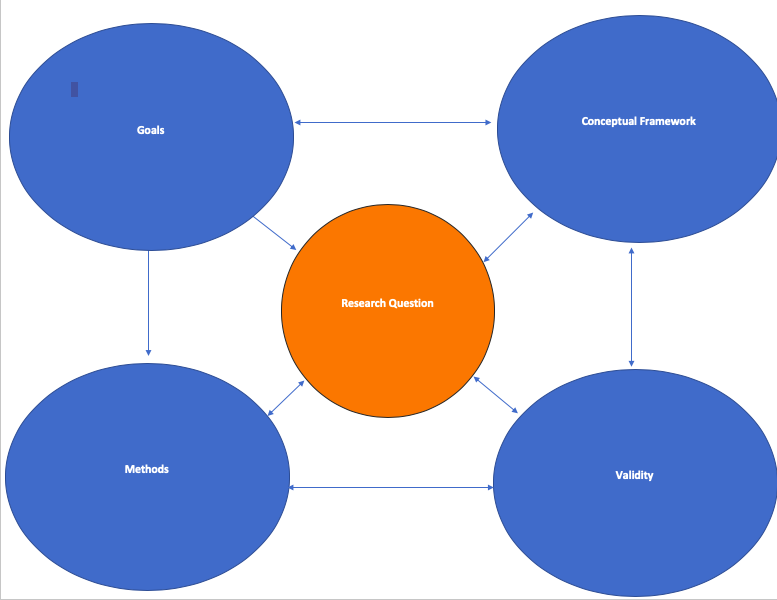
\includegraphics{images/questiondiagram.png}
\caption{Research Methods Diagram}\label{fig:questiondiagram}
}
\end{figure}

Focusing on the methods portion of the diagram, this chapter will discuss in
further detail each small n qualitative method.

\hypertarget{interviews}{%
\subsection{Interviews}\label{interviews}}

Conducting interviews can seem like a daunting experience. A researcher has to
develop a comfort in approaching diverse sets of people, many times in
unfamiliar environments. A researcher has to be able to build rapport, get
their questions answered within a limited amount of time and encourage the
participant to elaborate and clarify answers. Interviews are challenging but
the good news is there are ways to make the process smoother through
organization, commitment, and earnestness.

Before contacting anyone for an interview, a researcher should take sometime
to organize their interview guide and decide whether they want to conduct
structured or semi-structured interviews. The interview guide highlights the
questions and themes the researcher plans to cover during the interview. The
format of the interview guide is determined by whether the researcher has a
rigid structure of questions they plan to ask each participant (Structured
Interview) or a more flexible interview strategy that allows for the
researcher to deviate from questions and allow for a more exploratory
conversation within the confines of the research question (Semi-Structured
Interview).

Once a researcher has decided on an interview structure and completed their
interview guide, they can decide who they want to recruit to participate in
the interview. The researcher will need to consider the \textbf{key
informants} and \textbf{representative sample} they want to recruit. Key
informants are experts that can discuss the population of interest including
but not limited to academics, community leaders, and politicians. The
representative sample is the population that your research is based on. For
example, Wendy Pearlman's text \emph{We Crossed a Bridge and it Trembled:
Voices from Syria} has a representative sample of Syrians displaced during the
civil war (\protect\hyperlink{ref-pearlmanWeCrossedBridge2017}{Pearlman
2017}). What is important to understand about the difference between the
representative sample and key informants is that the sample is giving a
firsthand account of their experiences, while a key informant is mainly given
their observation and experiences of the representative sample from an outside
perspective.

Moving on to recruitment, Robert Weiss' \emph{Learning From Strangers} lists
several reasons that affect whether an individual is willing to participate in
an interview including: occupation, region, retirement status, vulnerability,
and sponsorship from others within their network
(\protect\hyperlink{ref-weiss1994a}{Weiss 1994}). Unfortunately, there is no
easy way to recruit but from experience face to face discussions with
potential participants and immediate follow up are quite effective. Also use
\textbf{snowball sampling} to use previous participants acquaintances and
networks to participate in interviews. These strategies are not full proof but
a layer of personal interaction through face to face contact or networks does
have advantages in making many people more receptive to participating in
interviews.

Lastly, when the day to interview finally arrives a researcher should have two
recorders, tissue, interview guide, consent form, and a gift card for the
participant if possible. The interview should not take any longer than an hour
as a sign of respect for the time of your participant. A researcher should
take meticulous notes during the interview. Also, the researcher must gain the
permission of the participant to conduct a follow up interview if necessary.

\begin{shaded*}

\textbf{Check-in Question 2:} What is this difference between a representative
sample and a key informant?

\end{shaded*}

\hypertarget{participant-observation}{%
\subsection{Participant Observation}\label{participant-observation}}

\textbf{Participant observation} is a variation of ethnographic research where
the researcher participates in an organization, community, or other
group-oriented activities as a member of the community. Typically used in
anthropology, it involves a researcher immersing themselves within a
community. Participant observation requires that the research build a strong
bond of trust with the observed community. A researcher (with the help of IRB)
will need to decide if participation will be active or passive and whether it
should be overt or covert. This can be a particularly sticky situation, as a
passive and covert observation may mean community members have no idea they
are being studied, while active and overt participation can lead to the
environment changing as the community is aware of the presence and role of the
researcher. Referring back to the work of Mary Pattillo, recall that she
eventually became a citizen of Groveland and participated as any other citizen
in community activities (\protect\hyperlink{ref-pattillo2013a}{Pattillo
2013}). This included leading the local church choir, joining the community's
local action group, and coaching cheerleading at the local park. Pattillo saw
her participant observations as essential to describing the black middle class
in Groveland and even speaks of the parallels between the Groveland
neighborhood and her upbringing in Milwaukee.

The key purpose of participant observations is to provide deeper insight into
process and how things function. This exercise is good for `theory building,'
but it may be best to include another method, such as interviewing, to allow
for the community to tell their story as well, a supplemental method Pattillo
uses as well. What is most important when using participant observation (in
qualitative methods in general) is to take meticulous field notes with
attention to accuracy. A researcher should be cognizant of their own biases
and constantly thinking through their analysis to make sure they a capturing
an accurate story. In order to tell an accurate story a researcher should keep
both mental notes and a notepad. After the end of an event it is important to
write everything down while the researcher's memory is fresh.

:::

\textbf{Check-in Question 3:} What are the advantages and disadvantage of
covert and over participant observation?

:::

\hypertarget{focus-groups}{%
\subsection{Focus Groups}\label{focus-groups}}

\textbf{Focus Groups,} similar to individual interviews requires a researchers
to set questions, recruit participants and follow up with participants as
necessary. As with an individual interview, the researcher should have an
interview guide to help structure the questions and themes of the focus group.
The advantage of a focus group is that a researcher is able to facilitate
multiple respondents at once, which can lead to additional details and
information you might not get in series of single interviews. As seen in
Melissa Harris Perry's \emph{Sister Citizen}, focus groups are great for
spurring discussion about topics such as stereotypes
(\protect\hyperlink{ref-harris-perry2011a}{Harris-Perry 2011}). A researcher
should note impressions, points of contention, and general interactions within
the group. Group dynamics and discussions can be used for theory building as
well as getting a deeper understanding of a particular group of people.

\hypertarget{process-tracing}{%
\subsection{Process Tracing}\label{process-tracing}}

\textbf{Process tracing} is a method of causal inference using descriptive
inference over time. Notably used by APD scholars, the goal of process tracing
are to collect evidence to evaluate a set of hypotheses through the framing of
historical events. There are four tests when discussing process tracing.

The first is the \textbf{straw in the wind test}. The straw in the wind test
can increase plausibility but cannot determine that any event necessary nor
sufficient criterion for rejecting. It can only weaken hypotheses. The
\textbf{hoop test} establishes necessary criterion. Though the hoop test does
not confirm any particular hypotheses, the test can eliminate hypotheses. The
\textbf{smoking gun test} provides a sufficient but not necessary criterion
for hypotheses. The test can give strong support for a given hypothesis and
can substantially weaken competing hypotheses. Lastly, the doubly decisive
test illustrates evidence that is necessary sufficient. Necessary being when
the necessary causes occur when the effect occur and sufficient being when
causes always occur after effects.

What is important to understand about process tracing beyond the numerous
tests is that process tracing is a good way in political science to draw
evidence for certain events and phenomena. Chloe Thurston uses process tracing
to track the development of the public-private partnership with regards to
housing policy (\protect\hyperlink{ref-thurston2018a}{Thurston 2018}). Through
numerous historical text including archives, testimonial, and presidential
records, Thurston is able to develop a story of how public-private
partnerships led to home owning policies that discriminated according to
gender, race, and socioeconomic status and how advocacy groups were able to
combat these policies.

Thus, process tracing looks for historical evidence to explain certain events
or policies.

\hypertarget{ethnography}{%
\subsection{Ethnography}\label{ethnography}}

\textbf{Ethnography} involves studying groups of people and their experiences
(\protect\hyperlink{ref-emerson2011a}{Emerson, Fretz, and Shaw 2011}). As
mentioned earlier with participant observations, the purpose of ethnography is
for a researcher to immerse themselves in the environment they are studying.
The researcher will need to develop relationships with the community and
detail the environment through constant note taking and reflection. This is
reflected in the work of many of the researchers already detailed in the
chapter. Done correctly a researcher can document the emotions, attitudes, and
relationships in a community that are sometimes impossible to capture in
quantitative work.

In his text \emph{Wounded City: Violent Turf Wars in a Chicago Barrio}, Robert
Vargas is able to capture the fear, frustration, and empowerment felt by the
residents of Chicago's Little Village as they negotiate turf wars between
gangs, police, and alderman {[}vargas2016a{]}. The insight he is able to
gather cannot simply be surveyed, but must be observed in the environment in
order to develop trust within the community.

Ethnography is about relationship building and allows for latent findings that
may give proper context for understanding particular groups. This is
especially important for underrepresented communities, where in depth research
is often lacking and responsiveness to a survey may not be likely under less
personal circumstances. Ethnography allows a researcher to take a more
holistic approach in understanding a community.

\begin{shaded*}

\textbf{Check-in Question 4:} What should a researcher be looking for when
taking ethnographic field notes?

\end{shaded*}

\hypertarget{applications-3}{%
\section{Applications}\label{applications-3}}

The application of small n qualitative methods is based on a researcher's
question. Sociologist, Celeste Watkins-Hayes, explains that qualitative
research is meant to tell specific stories about a community. Going back to
the diagram displayed in the beginning of the chapter, a researcher should
think of the story they are trying to tell and goals, whether the small n
qualitative methods they want to use are valid, and how does all of this
relate to the research question. Most importantly when applying small n
qualitative methods, record keeping is of the utmost importance. A researcher
should make sure that their field notes are detailed and capture an accurate
depiction of the environment of study. This means not only self-reflecting on
one's own biases, but also using multiple small n and quantitative methods
when appropriate to tell the most complete story possible. Lastly, a
researcher needs a method of coding the themes and messages found through
their study. Recording encounters and taking good field notes will go far in
creating an organized system, which will allow for a researcher to tell an
accurate story that captures the nuances and characteristics of a particular
community.

\hypertarget{advantages-of-method-3}{%
\section{Advantages of Method}\label{advantages-of-method-3}}

Small n qualitative research thrives with gaining in depth information about a
limited number of cases. This will allow a researcher to provide insight of a
small number of communities that may be missing from large n studies. In this
same breath, small n methods allow for theory building that many times is
unique to many of the lessons taken for granted in the discipline of political
science. It is one thing to ask an individual participant to check an answer
on a question about immigration, race, or president. Yet, there is value is
going deeper and wrestling with the values, contradictions, as well as the
historic and present-day context that make up the politics of a particular
people. It is through small n methods that researchers are able to get a
better understanding of topics such as rural consciousness, neighborhood
violence, and linked-fate. Small n methods allow a researcher to tell the
stories that are often ignored, unheard, or misinterpreted through other
methods.

\hypertarget{disadvantages-of-method-1}{%
\section{Disadvantages of Method}\label{disadvantages-of-method-1}}

The major disadvantage of small n methods is that a researcher is working from
a small pool. This should not be confused with having less data. Interviews,
field notes, and archives bring an abundance of data but the sources are
limited. A responsible researcher will have to consider whether their case
selection is representative of the broader community and how best to ensure
that they are getting a diverse set of voices to hear from to avoid inaccurate
assessments of a community. Thus, it is difficult (but not impossible) to
generalize from the use of small n research. A researcher including
quantitative methods or multiple small n methods in their study will go a long
way in strengthening their arguments.

\hypertarget{broader-significanceuse-in-political-science-4}{%
\section{Broader significance/use in political
science}\label{broader-significanceuse-in-political-science-4}}

As has been noted numerous times in the chapter, small n qualitative methods
allow a researcher to explore groups that cannot necessarily be understood
merely with a survey, experiment, or causal inference. Small n allows for a
researcher to go into more detail about groups that cannot be fully understood
through quantitative research either because they are too small or too
unresponsive to quantitative methods. Additionally, small n qualitative
research also allows for political scientist to consider context and history
when developing claims regarding the political behaviors and institutions that
shape society. This context can help a political scientist go beyond
superficial understandings of particular groups. For instance, Michael
Dawson's text \emph{Black Visions} uses quantitative methods to show that
African Americans have a high support for Black Nationalism
(\protect\hyperlink{ref-dawson2001a}{Dawson 2001}). This finding alone could
be taken as example of mass black prejudice, as Black Nationalism has been
associated most notably with the bigoted views of Louis Farrakhan. Yet, Dawson
takes care to include the historical context, including testimonials by
leading black thinkers, detailing the long history of debate concerning Black
Nationalism, as well as the economic violence and discrimination committed
against the black community, which leads to support of some forms of Black
Nationalism. Small n qualitative research through the use of history,
interviews, and ethnography allows for the telling of these stories, adding
complexity and nuance to many of political science's well established theories
and perceptions.

\hypertarget{conclusion-6}{%
\section{Conclusion}\label{conclusion-6}}

Not all questions can be answered with a survey and experiment alone.
Sometimes a deeper study into a community and event can lead to new and
exciting insights in the discipline of political science. Admittedly, small n
qualitative research can be met with some cynicism in certain parts of the
political science community, but when done correctly through meticulous note
taking, coding, and preparation small n qualitative methods can provide
insights that have yet to be fully articulated in the discipline and assist in
answering some of the most important questions of the day including policing,
immigration, and race relations.

\hypertarget{application-questions-7}{%
\section{Application Questions}\label{application-questions-7}}

\textbf{What are some materials needed to conduct small n research?}

\begin{shaded*}

A researcher should have their interview guide prepared, tissues, and two
recorders if conducting interviews or focus groups. Additionally, a researcher
should have a notepad for field notes and consent forms if necessary. Business
cards are also useful when trying to recruit participants from the field.

\end{shaded*}

\textbf{When in the field, how does a researcher build rapport with the community?}

\begin{shaded*}

Rapport can be built through appearance including dress, race, gender,
regional, and class markers. Most importantly, a researcher should present
themselves as engaged and attentive to the participants. A researcher should
remain professional and read the room, rapport building for a group of blue
collar workers may be different than with college students. A researcher
should remain cognizant of this distinction and look for openings to build
connections when possible.

\end{shaded*}

\hypertarget{social-networks}{%
\chapter{Social networks}\label{social-networks}}

\textbf{By Erin Ochoa}

\hypertarget{introduction-8}{%
\section{Introduction}\label{introduction-8}}

From microblogging with Twitter to leaving comments on YouTube videos, the use
of online social media platforms has become a part of everyday life for many:
as of January 2020, Kemp (\protect\hyperlink{ref-Kemp2020}{2020}) estimates
that there are 3.8 billion active social media users---49\% of the global
population. With the inception of social media---the precursors of which
arguably date to the 1970s, if not earlier---and its proliferation since the
turn of the millennium, interest has grown around the theory and methods for
analyzing data from such networking platforms. This type of research is a form
of \emph{social network analysis}.

Social networks among humans, however, have existed as long as humanity
itself. This is because a social network exists whenever two or more social
entities \emph{interact} or otherwise \emph{relate} to each another. Many such
interactions and relations in contemporary society are fleeting: transactions
between workers and customers in retail or service settings, strangers riding
a train together, or students in the same class whose acquaintanceship ends
along with the school year. Others may be formal, structured, deliberate, or
otherwise durable: members of a given Senate committee serving in a given term
of Congress, a hierarchy of workers in a company division, a marriage
relationship between spouses, or kinship ties. It is these formal, structured,
deliberate, and durable networks that are the primary focus of social network
analysis.

\hypertarget{what-is-a-social-network-what-is-social-network-analysis}{%
\section{What is a Social Network? What is Social Network
Analysis?}\label{what-is-a-social-network-what-is-social-network-analysis}}

A \textbf{social network} is a set of \emph{relationships} among \emph{social
entities}. \textbf{Social network analysis}, then, is a body of methods used
to evaluate the characteristics of social networks and their elements. To
better understand what these terms mean, it is important to first address what
a \emph{network} is and what elements it comprises. We will also consider
examples of networks and approaches to representing them.

\hypertarget{netElem}{%
\subsection{Elements of a Network}\label{netElem}}

A network is a set of \emph{entities} and the \emph{relationships} among them.
The study of networks is rooted in a sub-field of mathematics called
\emph{graph theory}. From this perspective, a \textbf{network} is a data
structure modeling a collection of units, which are represented as points
called \textbf{nodes} or \textbf{vertices}, and the relationships among them,
which are represented by links, called \textbf{edges} or \textbf{ties},
between the nodes. Two nodes that are connected by an edge are said to be
\textbf{neighbors}. A network is also called a \textbf{graph}; here, both
terms are used interchangeably.

Networks can represent many different types of real-world phenomena. Consider
how a network could be used to model each of the following:

\begin{itemize}
\item
  The genealogical history of the Japanese royal family:

  \begin{itemize}
  \tightlist
  \item
    Nodes represent people; ties represent marriages and births.
  \end{itemize}
\item
  Email correspondence between workers in a corporation:

  \begin{itemize}
  \tightlist
  \item
    Nodes represent workers; ties represent emails exchanged between pairs of
    workers.
  \end{itemize}
\item
  Flights between all the international airports in the world:

  \begin{itemize}
  \tightlist
  \item
    Nodes represent airports; ties represent flights connecting airports.
  \end{itemize}
\item
  Predator--prey relationships among animals in an ecosystem:

  \begin{itemize}
  \tightlist
  \item
    Nodes represent different species; ties represent which animals prey upon
    others.
  \end{itemize}
\item
  Mentorship and advising among political scientists in academia:

  \begin{itemize}
  \tightlist
  \item
    Nodes represent scholars; ties represent mentor--student relationships
    among scholars.
  \end{itemize}
\item
  The order in which blocks of code in a computer program could be executed:

  \begin{itemize}
  \tightlist
  \item
    Nodes represent blocks of code; ties represent flow control between
    blocks.
  \end{itemize}
\item
  Advice-seeking relationships among all current federal circuit judges in the
  United States:

  \begin{itemize}
  \tightlist
  \item
    Nodes represent judges; ties represent whether a given judge has ever
    asked another judge for advice.
  \end{itemize}
\end{itemize}

When the nodes in a network represent people, organizations, or another type
of social entity, the graph can be called a \textbf{social network}.

\hypertarget{network-representations}{%
\subsection{Network Representations}\label{network-representations}}

There are different ways to represent a network. The two most accessible
methods are sociograms and adjacency matrices. The sociogram in figure below
and the adjacency matrix in Table 11.1 are representations of the same
network.

\begin{figure}
\centering
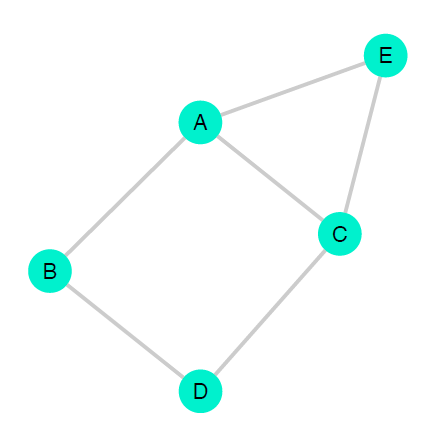
\includegraphics{images/social-networks/11-1.png}
\caption{A sociogram for a network with nodes {[}A, B, C, D, E{]}. Each circle
represents a node and each line represents a relationship between the two
nodes it connects}
\end{figure}

\begin{longtable}[]{@{}lccccc@{}}
\caption{Table 11.1: The adjacency matrix for a network with nodes
\([A, B, C, D, E]\). Rows and columns represent nodes; \(1\) denotes an edge
between two nodes and \(0\) denotes absence of edge, with dashes along the
diagonal to demonstrate that a node cannot have an edge to itself. In this
network, there exist relationships between nodes \(A \& B\), \(A \& C\),
\(A \& E\), \(B \& D\), \(C \& D\), and \(C \& E\).}\tabularnewline
\toprule
& \(A\) & \(B\) & \(C\) & \(D\) & \(E\) \\
\midrule
\endfirsthead
\toprule
& \(A\) & \(B\) & \(C\) & \(D\) & \(E\) \\
\midrule
\endhead
\(A\) & --- & \(1\) & \(1\) & \(0\) & \(1\) \\
\(B\) & \(1\) & --- & \(0\) & \(1\) & \(0\) \\
\(C\) & \(1\) & \(0\) & --- & \(1\) & \(1\) \\
\(D\) & \(0\) & \(1\) & \(1\) & --- & \(0\) \\
\(E\) & \(1\) & \(0\) & \(1\) & \(0\) & --- \\
\bottomrule
\end{longtable}

A sociogram is a diagram that displays the nodes as points and the edges as
lines or arrows.

To understand how an adjacency matrix works, first recall that a
\textbf{matrix} is a rectangular data structure containing numeric values
which are organized in rows and columns; the total number of \emph{cells} or
values in the matrix equals the number of rows multiplied by the number of
columns. An \textbf{adjacency matrix} is a square matrix that represents the
presence or absence of ties between pairs of nodes in a graph---it tells us
which nodes are \emph{adjacent}, that is, which nodes are neighbors. There
exists one row and one column for each node, and each cell value identifies
whether the nodes associated with that cell are adjacent.

\hypertarget{method-set-upoverview}{%
\section{Method: Set-up/Overview}\label{method-set-upoverview}}

\hypertarget{two-fundamental-network-attributes}{%
\subsection{Two Fundamental Network
Attributes}\label{two-fundamental-network-attributes}}

The two most fundamental attributes of a network are whether it is
\emph{directed} and whether it is \emph{weighted}.

\begin{figure}
\centering
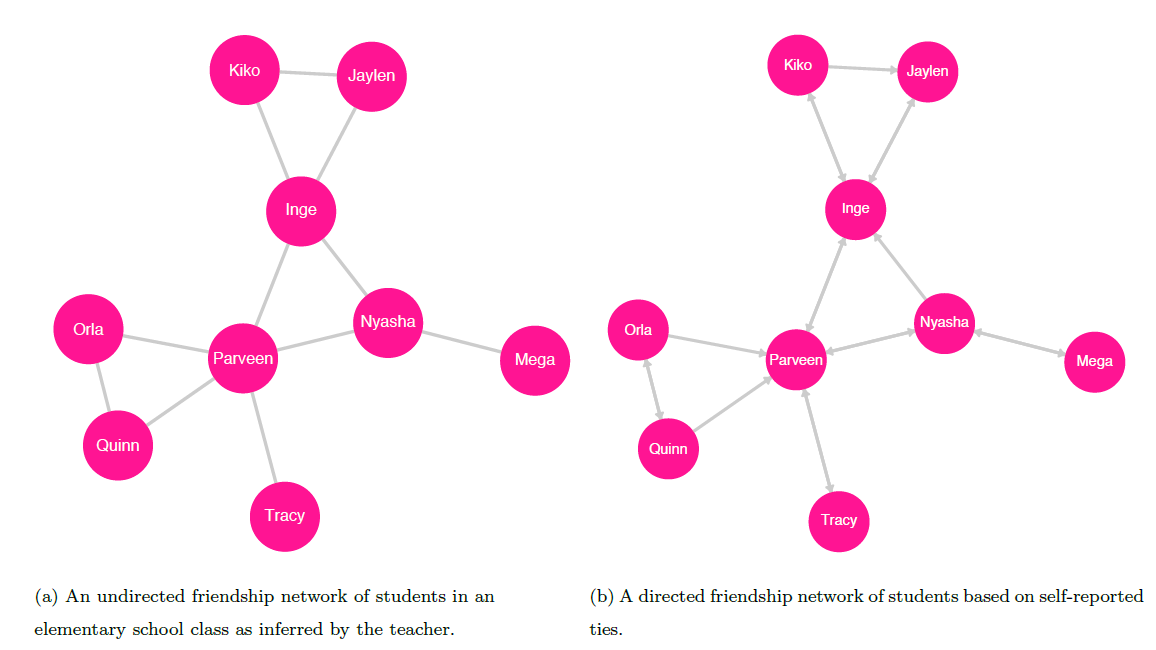
\includegraphics{images/social-networks/11-2.png}
\caption{An undirected (left) and directed (right) graph of a friendship
network among students. The ties in the undirected graph represent a mutual
friendship between pairs of students. For example, there is a tie between Orla
and Parveen, indicating that Orla is friends with Parveen and that Parveen is
friends with Orla\textbar their relationship is symmetric.}
\end{figure}

Note the arrows in the sociogram to the right; these indicate the direction of
perceived friendship from one node to another. For example: the two-way arrow
between Mega and Nyasha indicates that each considers the other a friend; the
one-way arrow pointing from Kiko to Jaylen, however, indicates that Kiko
considers Jaylen a friend, but also that Jaylen does not consider Kiko a
friend --their relationship is \emph{asymmetric}.

\textbf{Undirected and Directed Networks}

The first important attribute of a network is whether there is a direction
associated with the modeled relationships between nodes. There are two types
of graphs with respect to direction, \textbf{undirected} and
\textbf{directed}.

\textbf{Undirected Networks.} The most basic type is an undirected graph, in
which the edges represent \emph{symmetric}, or \emph{reciprocal},
relationships between nodes. The ties in an undirected graph are called
\textbf{undirected} or \textbf{symmetric ties}. Such ties indicate that for
any pair of connected nodes, both nodes have the same role in the
relationship.

One example of such a graph is the friendship network of students in an
elementary school class based on bonds observed by their teacher (see figure
above. In this network, an edge between two students means that their teacher
perceives them to have a mutual friendship; note that a tie does not indicate
any hierarchy among the connected nodes. If, for example, the teacher infers
that Inge and Jaylen are friends, then an undirected tie exists between them
in the graph. The edge between these two nodes means that to say \emph{Inge is
friends with Jaylen} is the same as saying \emph{Jaylen is friends with Inge}.

\textbf{Directed Networks.} In a directed graph, each tie has a direction: the
\textbf{directed ties} in a directed graph represent a \emph{one-way} or
\emph{asymmetric} relationship between nodes. We can think of asymmetric
relationships as those in which the roles of the source and destination nodes
differ.

Earlier, we described a network to model mentorship and advising between
political scientists (see figure below). For each tie in this network, one
node has the role of mentor and the other the role of student; note that each
node can take on one role or the other, or even \emph{both} depending on the
direction of its ties to other nodes. Let there be eight scholars in the
network: Akemi, Brett, Chi, Dani, Elvan, Farah, Gal, and Harvey. Akemi is the
most senior scholar and was an adviser to Brett and Chi when they were
graduate students. Later in their careers, Brett mentored Dani and Elvan, and
Chi mentored Farah, Gal, and Harvey. In this network, the direction of the tie
is a fundamental aspect of the relationship between two nodes: to say
\emph{Akemi mentors Brett} is not the same as saying \emph{Brett mentors
Akemi}.

A second example of a directed graph is the network of students in an
elementary school class based on friendship ties identified by the students
themselves 11.2: if Inge identifies Jaylen as a friend, then there exists a
friendship tie from Inge to Jaylen; if Jaylen identifies Inge as a friend,
then there exists a friendship tie from Jaylen to Inge. Kiko identifies both
Inge and Jaylen as friends, so there exist ties from Kiko to Inge and from
Kiko to Jaylen. Inge identifies Kiko as a friend, but Jaylen does not; thus,
there exists a tie from Inge to Kiko, but there is no tie from Jaylen to
Kiko---despite the tie from Kiko to Jaylen. The ability to denote such
asymmetric relationships is the key feature of directed graphs.

\begin{figure}
\centering
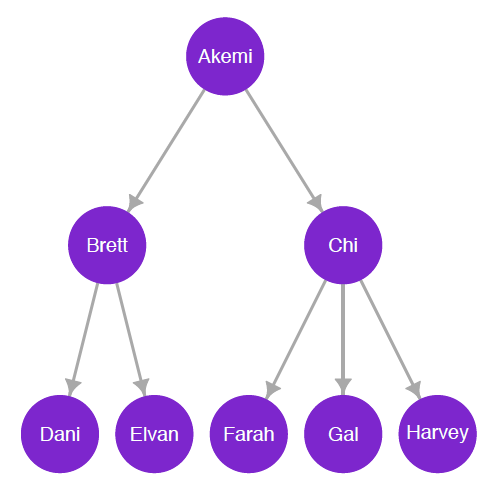
\includegraphics{images/social-networks/11-3.png}
\caption{A directed network of adviser--student relationships between
political scientists}
\end{figure}

\textbf{Weighting}

The second fundamental attribute of a graph is whether its ties are weighted.
There are two types of graphs with respect to weighting, \textbf{unweighted}
and \textbf{weighted}.

\textbf{Unweighted Networks.} In an unweighted graph, there are no values
associated with any of the edges. The relationships represented in the network
are modeled as equivalent, regardless of the circumstances surrounding each
relationship.

Consider the earlier example describing a friendship network among elementary
school classmates as observed by their teacher. In this undirected network, we
can consider ties as \emph{dichotomous} or \emph{binary}: between two nodes, a
tie either exists or not. Imagine that Inge and Jaylen have been neighbors,
friends, and classmates for five years, and both are now friends with Loren, a
new classmate who has recently moved to the neighborhood. In an unweighted
representation of the friendship network, the tie between Inge and Jaylen is
seen as equivalent to the tie between Inge and Loren: the network does not
capture the strength, duration, frequency of contact, or other qualities of
the friendship bonds, only whether the friendship bonds exist.

\textbf{Weighted Networks.} In a weighted graph, each edge has a numeric value
or \emph{weight} representing an attribute of the relationship between its two
nodes. Depending on the network, the value can measure the physical distance
between two nodes or some aspect of the strength or intensity of the
relationship between them or perhaps of the frequency of an event that occurs
between the two nodes.

A simple example of a weighted network is an undirected graph of several towns
and the highways existing between them. In this network, the weight of each
edge is the length of the highway connecting a pair of towns and thus measures
the distance between them.

For a directed weighted graph, recall the earlier example of the email
correspondence network among workers in a corporation. Consider the case of
two workers, Stéphane and Tracy, each of whom has sent emails to the other. To
make a directed weighted correspondence graph, assign to each edge the number
of emails sent by the source node to the destination node: Stéphane has sent
Tracy \(11\) emails, so the weight of the tie from Stéphane to Tracy is
\(11\); Tracy has sent Stéphane \(15\) emails, so the weight of the tie from
Tracy to Stéphane is \(15\). In this case, the edges represent the frequency
and direction of email contact between the two workers.

It is possible to convert a weighted directed graph to a weighted undirected
graph. This can be accomplished by summing the weights of ties between a pair
of nodes and assigning the result to a single undirected edge between the
nodes. For the email correspondence network, to replace the directed ties
between Stéphane and Tracy with an undirected tie, we add Stéphane's \(11\)
sent emails to Tracy's \(15\) and assign the value \(26\) to the link between
them. The edges now represent the frequency, but not the direction, of email
contact between Stéphane and Tracy.

\textbf{A Note on Node Attributes.} Real-world social entities vary in their
characteristics---that is, there are \emph{variables} associated with social
entities. For example, there exist many types of organizations, such as
non-profits, for-profit corporations, government agencies, and
intergovernmental bodies. Similarly, there are a plethora of aspects
associated with individual people. For example, consider the following: In the
United States, generally speaking, age cutoffs define the legal categories of
\emph{child} and \emph{adult}; persons with high-school degrees belong to one
category, while those who have not attained a high-school education belong to
a different one; and those with certain criminal convictions are labeled as
felons.

In general, each variable associated with a social actor measures a single
aspect of that actor: it may measure height or weight, but not both, for
example. These variables may be \emph{quantitative} (a \emph{number}, such as
the count of armed conflicts that have taken place in a district, or the fuel
efficiency of a vehicle in miles per gallon) or \emph{qualitative} (a
\emph{category}, such as a nation's form of government, or whether a state's
legal code allows for capital punishment). (For a thorough discussion of
variable types, see chapter on \emph{Data}.

We can represent the different values of a variable across the vertices in a
network using \emph{node attributes}. Here, we will only consider node
attributes that represent categorical variables, either nominal or ordinal. A
variable may take on a single value from a finite set of all possible
categories (the categories are \emph{exhaustive}), with each category being
distinct from all the others (the categories are \emph{mutually exclusive}).
Note, however, that discrete and continuous variables \emph{can} be converted
to ordinal variables by subsetting the possible values into categories.
Consider, for example, a variable that captures the count of shootings in a
neighborhood with categories such as 0-9, 10-19, 20-29, and \(\ge30\); or the
weight status associated with each range of BMI values as classified by the
CDC ((\protect\hyperlink{ref-CDC2017}{Centers for Disease Control and
Prevention 2017})): \(\le18.5\) is classified as \emph{underweight}, 18.5-24.9
as \emph{normal or healthy weight}, 25-29.9 as \emph{overweight}, and
\(\ge30\) as \emph{obese}.

In reality, social actors are associated with myriad characteristics,
conditions, and states of being. A given scientific study may measure many
such characteristics, with each constituting a single variable. While each
variable can only take on a single value for a given observation, a node in a
network may be associated with zero, one, or several variables. In the earlier
example of a friendship network among elementary-school students as inferred
by their teacher, there are no variables associated with any node: each vertex
represents a student, and no vertex attributes are taken into account. In the
case of organization types, each node has a \emph{type}, the categories of
which are (in this simplified case) \emph{non-profit}, \emph{for-profit},
\emph{governmental}, and \emph{intergovernmental}. As an example of a network
with two variables, consider a graph of ally relationships between
nation-states; the first variable captures whether the entity engaged in a
military conflict during the previous ten years (a binary variable that takes
the value \(True\) or \(False\)), and the second captures total per capita
military spending over that same period (an ordinal variable, with each
category capturing a range of spending amounts measured in thousands of
dollars, such as \([0, 10)\), \([10, 20)\), \([20, 30)\), \(\ge30\)).

To visualize node attributes in a network diagram, the physical aspects of a
node's presentation vary to represent different values; such aspects include
color, shape, and size. Sociograms with elements to represent more than two
attributes, however, become increasingly challenging to interpret with each
additional variable.

\hypertarget{network-node-measures-and-special-graphs}{%
\section{Network \& Node Measures and Special
Graphs}\label{network-node-measures-and-special-graphs}}

Now that we have covered the foundations of graph elements, we can consider
some concepts often implemented in the study social networks. We begin by
describing key characteristics that apply to an entire graph, followed by
definitions of node-specific measures. We then introduce some special types of
graphs.

\begin{figure}
\centering
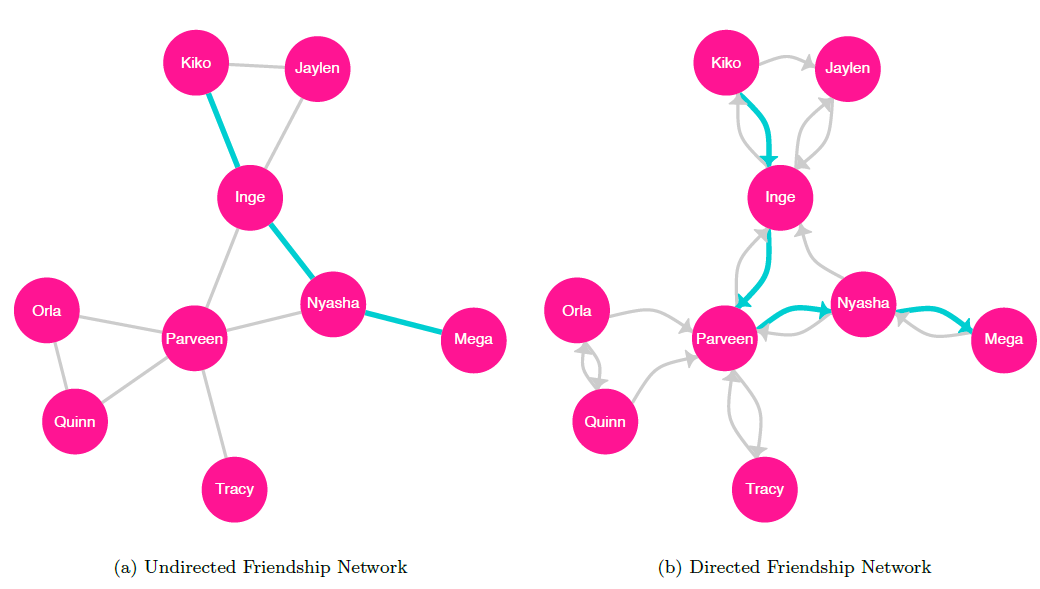
\includegraphics{images/social-networks/11-4.png}
\caption{Sociograms for undirected (left) and directed (right) graphs with
highlighted geodesics between Kiko and Mega}
\end{figure}

\hypertarget{graph-characteristics}{%
\subsection{Graph Characteristics}\label{graph-characteristics}}

\textbf{Distance}

There are many important concepts related to the traversal of a graph from one
specific node to another. To traverse a graph from one node to another, we
follow a \textbf{path}, a sequence of nodes connected by edges, spanning from
an origin node to a destination node without repeating any nodes or edges
(\protect\hyperlink{ref-WassermanFaust1994}{Wasserman and Faust 1994}). For a
directed graph, the path follows the direction of each edge. Note that for any
pair of nodes in a network, there may exist multiple paths.

The \textbf{path length} is the number of edges in a given path between two
nodes, and the shortest path between two given nodes is called their
\textbf{geodesic} (\protect\hyperlink{ref-WassermanFaust1994}{Wasserman and
Faust 1994}). The sociograms below highlight the geodesics between Kiko and
Mega for both undirected and directed representations of the student
friendship network.

The \textbf{distance} between any two nodes, also referred to as the
\emph{geodesic distance} is the length of their geodesic. For example, if
nodes \(A\) and \(B\) are connected by an undirected tie, then their geodesic
distance is \(1\).

We can find the \textbf{mean path length}, also called the \textbf{average
path length} or \textbf{characteristic path length}, by averaging the geodesic
distances between all pairs of nodes in the graph
(\protect\hyperlink{ref-WattsStrogatz1998}{Watts and Strogatz 1998}).

The \textbf{diameter} of a network is the maximum geodesic distance between
any two vertices in the network
(\protect\hyperlink{ref-WassermanFaust1994}{Wasserman and Faust 1994}). Note
that the path under evaluation is \emph{not necessarily} the \emph{longest
path} between any two vertices, but the longest of the geodesic paths in the
graph.

\begin{figure}
\centering
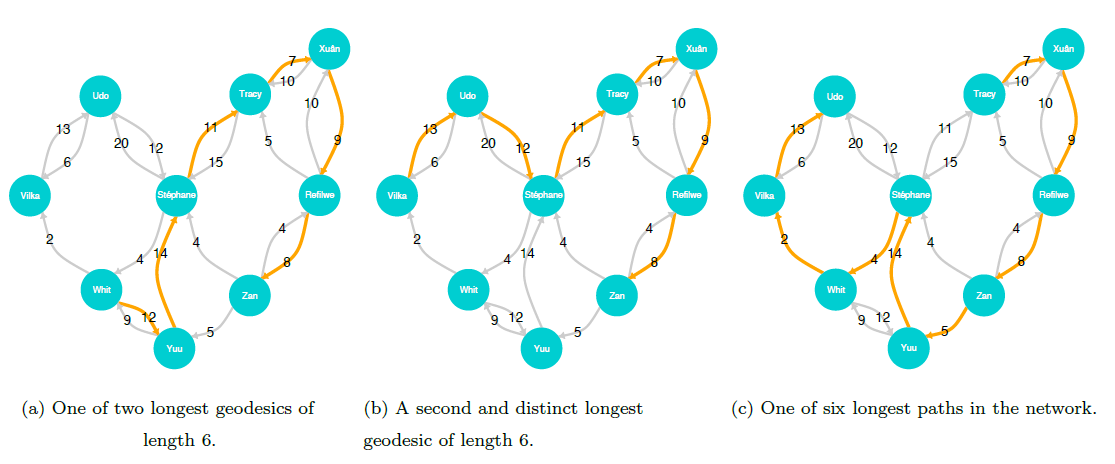
\includegraphics{images/social-networks/11-5.png}
\caption{Sociograms for the two longest geodesics (left and center) in the
directed weighted email correspondence network and one of the six longest
paths (right). The path length of each of the geodesics is 6, meaning that the
diameter of the graph is 6. Visiting each node only once, there are six
longest paths, each of length 8. Note that because the graph is directed, the
paths in each sociogram must follow the directions of the arrows}
\end{figure}

\textbf{Subgraphs and Components}

A network in which each node is directly connected to all the other nodes is
called a \textbf{complete graph} (see figure below; this is a special case of
a \textbf{geographic network}, which we will describe later.

A graph in which each node can reach all other nodes via a path is called a
\textbf{connected graph} (\protect\hyperlink{ref-WassermanFaust1994}{Wasserman
and Faust 1994}). The graphs shown in the above figures are connected graphs.
Note that while not every connected graph is a complete graph, all complete
graphs are connected graphs.

If we take a subset of the nodes in a graph, including some or all of the
edges among the subset of nodes (or, alternately, a subset of edges and all
the nodes attached to those edges), the result, called a \textbf{subgraph}, is
itself a graph (\protect\hyperlink{ref-WassermanFaust1994}{Wasserman and Faust
1994}).

Wasserman and Faust (\protect\hyperlink{ref-WassermanFaust1994}{1994}) define
three main categories of subgraphs (based on the number of nodes they contain)
with special names: \textbf{isolates}, \textbf{dyads}, and \textbf{triads}. An
isolate is a single node that is not connected to any other nodes. A dyad is a
subgraph of two nodes, either connected or not. A triad is a subgraph of three
nodes; in an undirected graph, there may be zero and three edges among the
nodes. Note that dyads and triads can include isolates.

If a subgraph is a connected graph---if every node is reachable from every
other node---\emph{and} there are no other nodes connected to the subgraph,
then the subgraph is called a \textbf{connected component}. This means that a
subgraph consisting of a single node---an isolate---is considered a connected
component. Every graph has at least one connected component.

A \textbf{disconnected graph} is one in which at least one node is not
reachable via a path from at least one other node
(\protect\hyperlink{ref-WassermanFaust1994}{Wasserman and Faust 1994}). An
equivalent definition describes a disconnected network as one in which at
least one connected component is not reachable from another. This means that a
disconnected graph has at least two connected components. The network shown
below is a disconnected graph with three connected components.

\begin{figure}
\centering
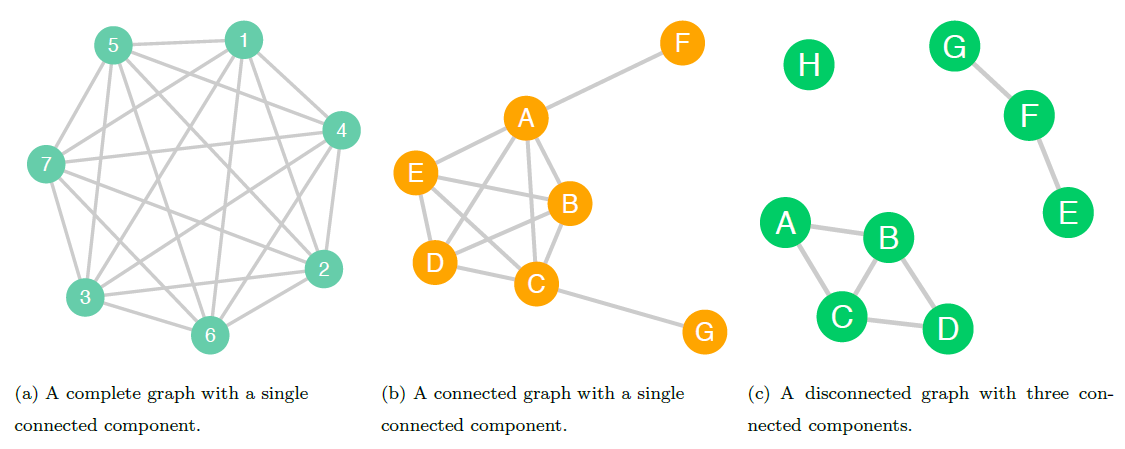
\includegraphics{images/social-networks/11-6.png}
\caption{In the complete graph (left), each node is directly connected to all
the other nodes; this graph is also a complete graph. In the connected graph
in the center, each node is reachable from all other nodes in the graph. The
disconnected graph (right) has three connected components; there is no way to
get from some nodes to certain others}
\end{figure}

\hypertarget{node-specific-measures}{%
\subsection{Node-specific Measures}\label{node-specific-measures}}

\textbf{Centrality}

A node's \textbf{centrality} can be used to gauge how important it is, for
various conceptualizations of \emph{importance}. There are many different
measures of centrality; here, we will discuss three such measures:
\textbf{betweenness centrality}, \textbf{closeness centrality}, and
\textbf{degree centrality}.

Note that though these metrics can be computed for all nodes in a graph, they
only make sense for nodes within a connected component; this is because the
distance between nodes that are not connected is undefined. These
node-specific measures are therefore only computed based on the other nodes in
a given node's connected component Recall, however, that a connected graph
contains a single connected component in which each node is connected to all
others.

\textbf{Betweenness centrality.} The \textbf{betweenness centrality} metric
evaluates a given node's ability to create connections \emph{between} other
nodes. According to Freeman, who formalized the definition of the metric,
betweenness is important because ``a vertex falling between two others can
facilitate, block, distort, or falsify communication between the two; it can
more or less completely control their communication''
((\protect\hyperlink{ref-Freeman1977}{Freeman 1977, 36})). For a given target
node, betweenness centrality is found by computing the sum, for all other
pairs of nodes in the component, of the ratio of the number of geodesics
between the pair of nodes that pass through the target node to the total
number of geodesics between the pair of nodes
(\protect\hyperlink{ref-Freeman1977}{Freeman 1977}). More formally, we can
write the definition of betweenness for a node \(v\) as:
\[Betweenness(v) = \sum_{i \neq j \neq v}^{n}\frac{g_{ij}(v)}{g_{ij}}\] where
\(g_{ij}\) is the number of geodesics between node \(i\) and node \(j\), and
\(g_{ij}(v)\) is the number of such paths that pass through node \(v\)
(\protect\hyperlink{ref-Freeman1977}{Freeman 1977}). The graph below displays
each node's betweenness.

\begin{figure}
\centering
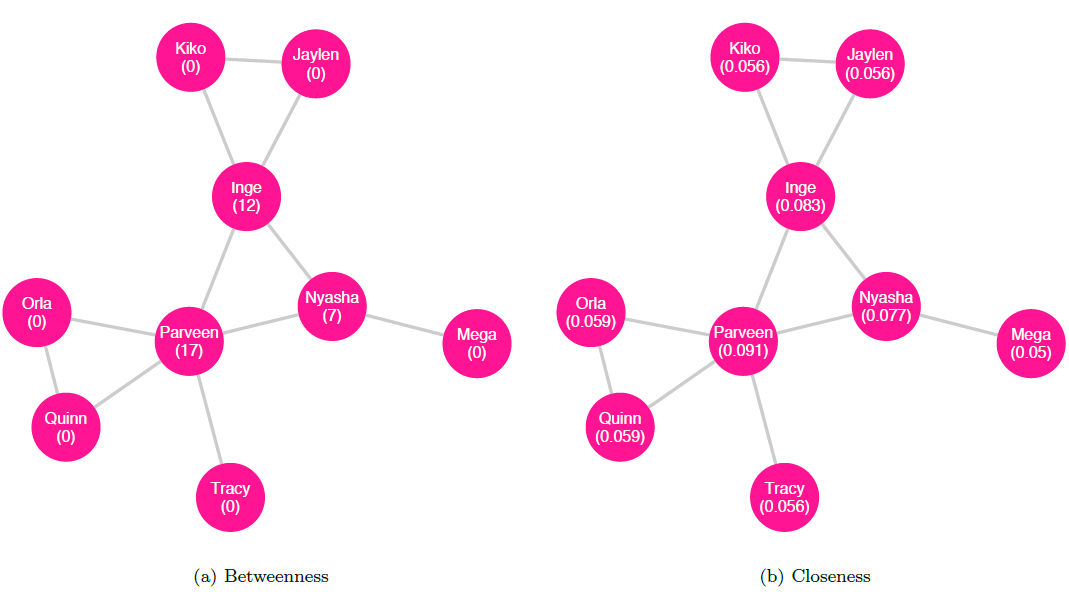
\includegraphics{images/social-networks/11-7.png}
\caption{Betweenness (left) and closeness (right) for the undirected
friendship network. Note that Parveen has the highest value for each measure}
\end{figure}

\textbf{Closeness centrality.} \textbf{Closeness centrality} measures how
\emph{close} a node is to others. For a given node in a connected component,
closeness centrality is found by computing the reciprocal of the sum of all
the distances between the given node and each other node in the component. We
can write the definition of closeness for a node \(v\) thus:
\[Closeness(v) = \frac{1}{\sum_{i \neq v}^{n}d(v, i)}\] where \(d(v, i)\) is
the geodesic distance between nodes \(v\) and \(i\)
(\protect\hyperlink{ref-WassermanFaust1994}{Wasserman and Faust 1994}). The
network in figure above displays each node's closeness centrality.

\textbf{Degree centrality.} A third measure of centrality is \textbf{degree
centrality}, which considers important nodes to be those that have many
neighbors. The \textbf{degree} of a vertex tells us its number of neighbors.
To calculate the degree of a vertex in an undirected graph, we can simply
count the number of edges it has
(\protect\hyperlink{ref-WassermanFaust1994}{Wasserman and Faust 1994}). Let us
return to the example of an undirected friendship network among classmates as
inferred by the teacher (shown in figure @ref(fig:fig11-8) with each node's
degree labeled); in this network, if Parveen is connected to Inge, Nyasha,
Orla, Quinn, and Tracy, then Parveen has a degree of \(5\).

\begin{figure}
\hypertarget{fig:11-8}{%
\centering
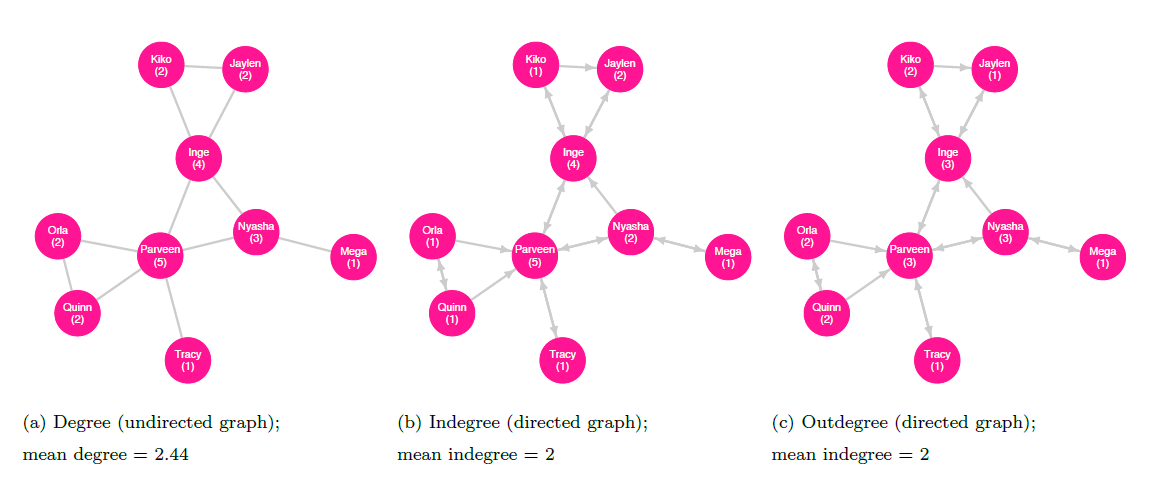
\includegraphics{images/social-networks/11-8.png}
\caption{Degree as measured in undirected (left) and directed (indegree,
center; and outdegree, right) networks}\label{fig:11-8}
}
\end{figure}

For a directed graph, a node's \textbf{indegree} is the number of edges
terminating there; the \textbf{outdegree} is the number of edges originating
from the node (\protect\hyperlink{ref-WassermanFaust1994}{Wasserman and Faust
1994}). As an example, we can consider the directed friendship network as
described by the students (shown with indegree and outdegree labeled in
figures @ref(fig:fig11-8) and @ref(fig:fig11-9), respectively). In this
network, the students Inge, Nyasha, Orla, Quinn, and Tracy consider Parveen to
be a friend, so Parveen has an indegree of \(5\). Parveen, in turn, considers
only Inge, Nyasha, and Tracy to be friends and so has an outdegree of \(3\).

A network's \textbf{degree distribution} describes the probability of a given
node in the graph having a degree of a certain value. In practical terms, we
can think of it as a set of numbers, where each reflects the count of nodes in
the graph with degree of \(0\), degree of \(1\), degree of \(2\), and so on.
The degree distribution for the undirected friendship network is displayed in
figure @ref(fig:fig11-9). The concept of degree distribution will be important
later when we discuss \emph{power-law networks}.

The \textbf{mean degree} of a graph is the mean average of the degrees for all
the vertices in the entire graph
(\protect\hyperlink{ref-WassermanFaust1994}{Wasserman and Faust 1994}). For
example, if an undirected network has four nodes with degrees
\([1, 1, 2, 2]\), then the mean degree for the network is \(1.5\). If a
directed graph has five nodes with indegrees \([0, 1, 3, 3, 3]\), and
outdegrees \([1, 2, 2, 2, 3]\), then the mean of the indegrees is \(2\) and
the mean of the outdegrees is also \(2\); note that these are equal because
every edge extending from some node points to another
(\protect\hyperlink{ref-WassermanFaust1994}{Wasserman and Faust 1994}).

\textbf{Clustering}

In order to evaluate clustering within a network, we must first introduce the
notion of a \textbf{triple}, sometimes called a \textbf{triplet}, which is a
connected component with three nodes---that is, it's a triad with at least two
edges. If a triple forms a complete graph---that is, if each node is connected
to both the others---then it is a \textbf{closed triple}, also known as a
\textbf{triangle}; otherwise, one pair of nodes in the triple are not adjacent
so it is an \textbf{open triple}. An \textbf{ordered triple} is one for which
the vertex order is a characteristic of the triple; for example, if the
vertices \([A, B, C]\) form a triangle, the ordered triples \(ABC\), \(ACB\),
\(BAC\), \(BCA\), \(CAB\), and \(CBA\) are each distinct---but note that the
\emph{triangles} formed by each triple are all the same.

\begin{figure}
\hypertarget{fig:fig11-9}{%
\centering
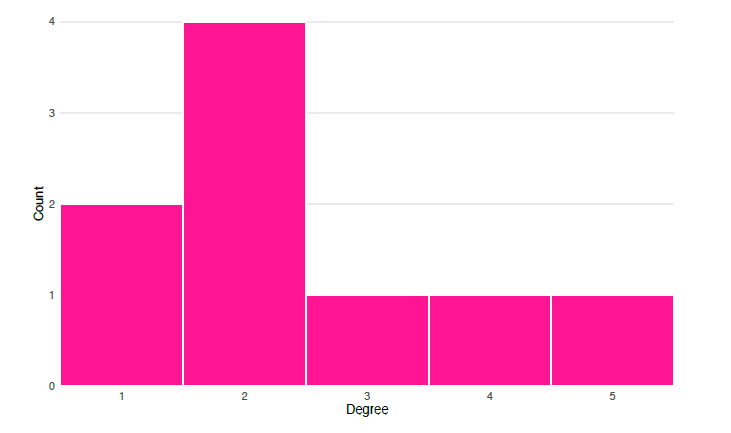
\includegraphics{images/social-networks/11-9.png}
\caption{A histogram of the degree distribution for the undirected friendship
network shows that there are two nodes with degree \(1\), four with degree
\(2\), and one each with degrees \(3\), \(4\), or \(5\)}\label{fig:fig11-9}
}
\end{figure}

For our purposes, we will assume that all edges are \emph{undirected} when
considering triples, triangles, and clustering. Note that in many applications
outside the scope of this chapter, this assumption will not hold.

We can now define, for any given node, its \textbf{local clustering
coefficient} (also called the \textbf{local transitivity}) by taking the
fraction of the pairs of the node's neighbors that are in turn neighbors with
one another---that is, the number of triangles including the node divided by
the number of possible triangles
(\protect\hyperlink{ref-WattsStrogatz1998}{Watts and Strogatz 1998};
\protect\hyperlink{ref-Opsahl2013}{Opsahl 2013}). An equivalent definition
given in Saramäki et al.~((\protect\hyperlink{ref-SaramakiEtAl2007}{Saramäki
et al. 2007})) is to compute the ratio of twice the number of triangles that
include the given node to the product of the node's degree and one less than
its degree:

\[Transitivity_{local}(v) = \frac{2 \times t_v}{degree(v) \times (degree(v) - 1)}\]
where \(t_v\) is the number of triangles that include node \(v\). (Note that
for nodes with degree of 1, this results in a zero in the denominator, which
means that local transitivity is undefined for such nodes. However, for the
purposes of computing the average local clustering coefficient, these
undefined values can be replaced with \(0\).) This metric measures cohesion
among a given vertex and its neighbors
(\protect\hyperlink{ref-BarratEtAl2004}{Barrat et al. 2004}). The local
transitivity for nodes in the undirected friendship network is shown in figure
@ref(fig:fig11-10) (with undefined values replaced with \(0\)).

We can compute the average local clustering coefficient for a graph \(g\) by
taking the mean across all nodes:
\[AverageLocalTransitivity(g) = \frac{\sum_{i = 1}^{N}Transitivity_{local}(n_i)}{N}\]
where \(n_i\) represents a node identified by its index and \(N\) is the
number of nodes in the entire network
(\protect\hyperlink{ref-BarratEtAl2004}{Barrat et al. 2004}). According to
Barrat et al. (\protect\hyperlink{ref-BarratEtAl2004}{2004}), this measure
``expresses the statistical level of cohesiveness measuring the global density
of interconnected vertex triples in the network''
((\protect\hyperlink{ref-BarratEtAl2004}{Barrat et al. 2004, 3750})).

Finally, to calculate the \textbf{global clustering coefficient}, also called
the \textbf{global transitivity}, for a graph \(g\), we take the ratio of
thrice the number of triangles to the number of all ordered triples---both
closed and open---in the graph:
\[Transitivity_{global}(g) = \frac{3 \times Triangles(g)}{Triples_{ordered}(g)}\]
where \(Triangles(g)\) is the total number of triangles in graph \(g\) and
\(Triples_{ordered}(g)\) is the total number of ordered triples in \(g\)
(\protect\hyperlink{ref-Opsahl2013}{Opsahl 2013}).

\begin{figure}
\hypertarget{fig:fig11-10}{%
\centering
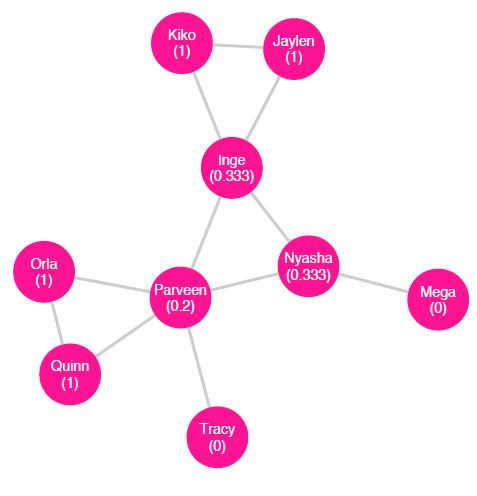
\includegraphics{images/social-networks/11-10.png}
\caption{Local transitivity for the undirected friendship network (with global
transitivity = \(0.3913\) and average local transitivity =
\(0.5407\))}\label{fig:fig11-10}
}
\end{figure}

\textbf{Density}

The \textbf{density} of a network is the ratio of the number of edges it
contains to the number of \emph{possible} edges. For example, in a network of
seven nodes, the number of possible edges is found by the combination
\(7C_2 = \frac{7!}{2!(7 - 2)!} = 21\). If there exist \(12\) edges among the
nodes, then the density of the network is \(\frac{12}{21} = .57\) or \(57\%\).

\hypertarget{special-graphs}{%
\subsection{Special Graphs}\label{special-graphs}}

\textbf{Geographic Networks}

A \textbf{geographic network} is one in which each node is connected to the
\emph{k} nearest nodes, with \emph{k} ranging from \(1\) to the total number
of nodes in the network minus \(1\). If \emph{k} takes on the maximum
value---that is, if each node is connected to all the other nodes---then the
network is called a \textbf{complete graph}. figure @ref(fig:fig11-11) shows a
geographic network with \(k = 4\).

\begin{figure}
\hypertarget{fig:fig11-11}{%
\centering
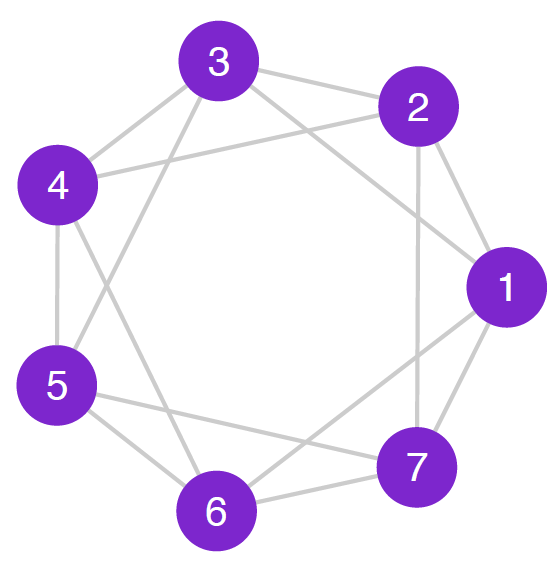
\includegraphics{images/social-networks/11-11.png}
\caption{A geographic network with \(k = 4\). Each node is connected to its
four closest neighbors}\label{fig:fig11-11}
}
\end{figure}

\textbf{Random Networks}

A \textbf{random network} is one in which, for each pair of nodes, there is a
probability \(p\) that there is an edge between them. This probability is a
constant for the entire graph and can range from \(0\) to \(1\). The sociogram
in figure @ref(fig:fig11-12) shows a random graph of \(15\) nodes and
probability \(p = 0.2\).

\textbf{Small-World Networks}

The small-world phenomenon describes the idea that in a large population, most
people are connected to each other by relatively short chains of
acquaintances. In a series of widely known experiments conducted within the
United States, Milgram and Travers asked arbitrarily chosen participants to
attempt to make contact with a specific target person by mailing or delivering
a provided document to someone the participant knew on a first-name basis who
was more likely to be personally acquainted with the target person; their
findings in one experiment showed that among successful contacts, the average
number of intermediaries between the initial participants and the target
person was \(5.2\) (\protect\hyperlink{ref-Milgram1967}{Milgram 1967};
\protect\hyperlink{ref-MilgramTravers1969}{Milgram and Travers 1969}). Dodds,
Muhamad, and Watts (\protect\hyperlink{ref-DoddsEtAl2003}{2003}) conducted an
international email study in a similar vein, finding that successful contacts
were transmitted across an average chain length of \(4.05\) steps.; when
accounting for attrition, they found a median chain length of \(7\) steps.

These experiments show that the small-world hypothesis appears to be
consistent with society at large: in just a few degrees of separation, one's
network of friends of friends grows very large.

Small-world networks exhibit two key characteristics: (1) the mean local
clustering coefficient is high---that is, on average, a node's neighbors are
highly connected to each other
(\protect\hyperlink{ref-WattsStrogatz1998}{Watts and Strogatz 1998}); and (2)
the mean geodesic distance is low---that is, on average, the distance between
nodes is short(\protect\hyperlink{ref-WattsStrogatz1998}{Watts and Strogatz
1998}). Given high average clustering, we might expect such networks to be
dense, but in fact, they tend to have relatively few edges
(\protect\hyperlink{ref-TakesKosters2011}{Takes and Kosters 2011}). Because
they have a small mean path length, the diameter---the largest geodesic
distance between any two nodes---is ``exponentially smaller than the size of
the network'' (\protect\hyperlink{ref-Kleinberg2000}{Kleinberg 2000, 845}).

\begin{figure}
\hypertarget{fig:fig11-12}{%
\centering
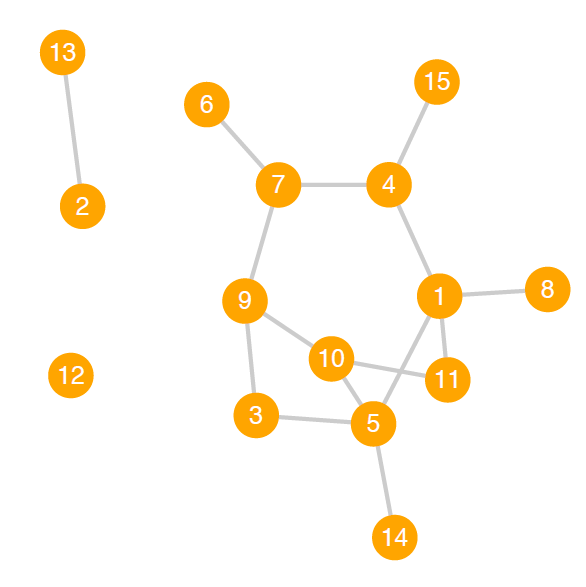
\includegraphics{images/social-networks/11-12.png}
\caption{A random network with N = 15 and p = 0:2}\label{fig:fig11-12}
}
\end{figure}

The combination of these features results in a network through which
information, preferences, and other conditions (such as infectious disease)
can diffuse quickly (\protect\hyperlink{ref-WattsStrogatz1998}{Watts and
Strogatz 1998}).

Figure @ref(fig:fig11-13) shows two representations of the same small-world
network, one with a diameter of \(4\), mean degree centrality of \(3.1\) and a
global clustering coefficient of \(0.155\).

\textbf{Power-Law Networks}

A \emph{power-law function} is a relationship between two variables, \(x\) and
\(y\), of the form \(y = cx ^ a\), where \(a\) and \(c\) are constants. This
equation models \(y\) as proportional to \(x ^ a\); as \(x\) changes, \(y\)
changes equal to the scale of \(x ^ a\), which is \(c\). The exponent \(a\)
can be any real number (though \(a = 0\) yields a horizontal line and
\(a = 1\) yields a diagonal line).

\textbf{Power-law networks} are those in which the degree distribution
approximates a special case of the power-law function where the scale constant
\(c = 1\) (thus why such networks are sometimes called \textbf{scale-free
networks}) and the exponent is negative: \(P(x) = x ^ {-a}\). In power-law
graphs, the degree distribution shows a large number of low-degree nodes (on
the left side of the distribution) and a small number of nodes with very high
degree (on the right side of the distribution). As Kadushin notes, for social
networks following a power-law distribution, the exponent \(a\) ``generally
lies between \(2\) and \(3\)'' ((\protect\hyperlink{ref-Kadushin2012}{Kadushin
2012, 114})).

Scientific studies across a variety of disciplines have indicated that
power-law networks abound; Newman, for instance, comments on the ``ubiquity of
power-law behaviour in the natural world''
(\protect\hyperlink{ref-Newman2005}{Newman 2005}). In new research, however,
Broido and Clauset challenge the general belief that power-law networks are as
widespread as many have claimed, finding specifically that ``social networks
are at best weakly scale free, and although a power-law distribution can be a
statistically plausible model for these networks, it is often not a better
model than a non-scale-free distribution''
((\protect\hyperlink{ref-BroidoClauset2019}{Broido and Clauset 2019})).

\begin{figure}
\hypertarget{fig:fig11-13}{%
\centering
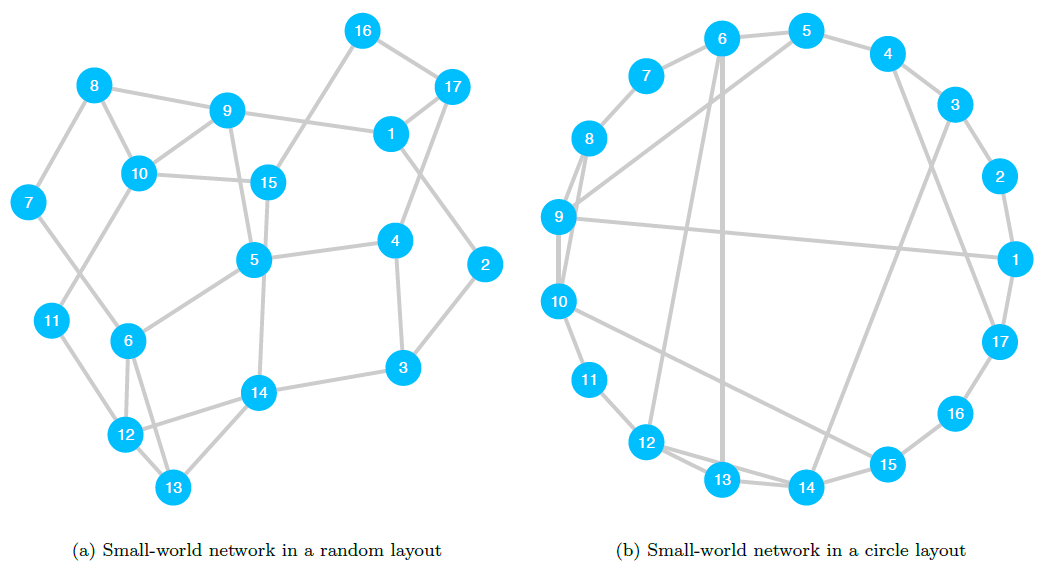
\includegraphics{images/social-networks/11-13.png}
\caption{Sociograms of a single small-world network with N = 17 nodes. This
graph has a diameter of 4, mean degree centrality of 3:1 and a global
clustering coefficient of 0:155}\label{fig:fig11-13}
}
\end{figure}

\hypertarget{applications-of-social-network-analysis}{%
\section{Applications of Social Network
Analysis}\label{applications-of-social-network-analysis}}

Here we describe in detail two studies of social networks in the domain of
political science.

\hypertarget{detecting-political-homophily-on-twitter}{%
\subsection{Detecting Political Homophily on
Twitter}\label{detecting-political-homophily-on-twitter}}

(\protect\hyperlink{ref-ColleoniEtAl2014}{Colleoni, Rozza, and Arvidsson
2014}) analyze the networks of Twitter users in an effort to measure
homophily---the extent to which nodes are linked to others with which they
share a given characteristic---among Democrats compared to that among
Republicans. Their primary research question (p.~317) focuses on the nature of
online social news platforms: do these provide their users access to diverse
political discourse (the \emph{public sphere} scenario), or are they more
likely to insulate users from others with differing political orientations
(the \emph{echo chamber} scenario)?

The authors implement a machine learning algorithm for an introduction to
machine learning methods) to label a set of Twitter users (the \emph{egos}) by
their political leaning based on the content of their politically oriented
tweets. Using the same classification method, they identify the egos'
neighbors based on outgoing ties---the users whom the ego \emph{follows} on
Twitter (the \emph{alters})---as either Democrats or Republicans (with alters
found to be non-political excluded). The result is a directed \emph{ego
network} around each ego, with alters labeled according to their own political
leaning.

\begin{figure}
\hypertarget{fig:fig11-14}{%
\centering
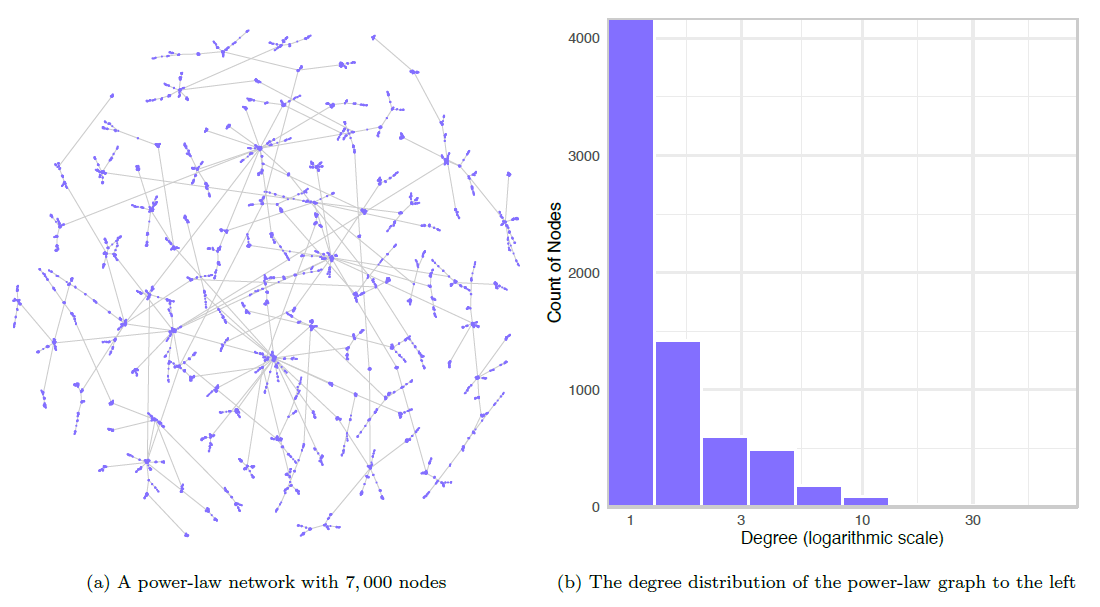
\includegraphics{images/social-networks/11-14.png}
\caption{A sociogram and histogram of the corresponding degree distribution
for a power-law network}\label{fig:fig11-14}
}
\end{figure}

Next, the researchers calculate each ego's homophily thus: ``the homophily
rate is defined as the number of outbound ties directed to alters who share
political orientation, divided by the overall number of outbound ties (i.e.,
directed to alters with similar political orientation plus directed to alters
with different political orientation)''
(\protect\hyperlink{ref-ColleoniEtAl2014}{Colleoni, Rozza, and Arvidsson 2014,
324}). We can write their equation for homophily as:
\[homophily(ego_i) = \frac{alters_{i.s}}{alters_{i.t}}\] where
\(alters_{i.s}\) is, for ego \(i\), the number of alters with the same
political orientation and \(alters_{i.t}\) is the total number of politically
oriented alters. Higher values of homophily (that is, greater than \(0.5\))
mean that a given ego is connected to a greater proportion of alters who share
the ego's political orientation compared to the proportion of alters with the
other orientation.

Finally, the authors create two subgraphs: the first is a network of egos and
their reciprocal alters (that is, the alters who also follow the ego); this
graph represents Twitter as a \emph{social platform} in which users form
reciprocal relationships with other users. The second is a network of egos and
their asymmetric ties (that is, the alters who do not follow the ego); this
graph represents Twitter as a \emph{news platform} in which egos follow
accounts that disseminate information, while those accounts do not form a
relationship with the ego (Colleoni et al.
(\protect\hyperlink{ref-ColleoniEtAl2014}{Colleoni, Rozza, and Arvidsson 2014,
320--21})).

With regard to their main research question---is Twitter a public sphere or
echo chamber?---the authors find that the results are contingent on whether
Twitter is conceptualized as a social or news platform: ``If we look at
Twitter as a social medium we see higher levels of homophily and a more echo
chamber-like structure of communication. But if we instead focus on Twitter as
a news medium, looking at information diffusion regardless of social ties, we
see lower levels of homophily and a more public sphere-like scenario''
(\protect\hyperlink{ref-ColleoniEtAl2014}{Colleoni, Rozza, and Arvidsson 2014,
328}). This means that the subgraph of reciprocal ties exhibits higher levels
of users who are mutually connected to other users sharing their political
ideology. The subgraph of asymmetric ties instead exhibits lower levels of
homophily, indicating that users \emph{are} being exposed to diverse political
news and opinions.

\hypertarget{measuring-the-effect-of-centrality-on-advocacy-output-in-a-network-of-transnational-human-rights-organizations}{%
\subsection{Measuring the Effect of Centrality on Advocacy Output in a Network
of Transnational Human Rights
Organizations}\label{measuring-the-effect-of-centrality-on-advocacy-output-in-a-network-of-transnational-human-rights-organizations}}

(\protect\hyperlink{ref-Murdie2014}{Murdie 2014}) explores a network of
transnational human rights organizations to assess whether an organization's
position in the network affects their level of political activity. The primary
research question is whether an organization's influence score affects its
advocacy output. The author hypothesizes that organizations with high
influence scores will engage in more advocacy events.

Murdie constructs a directed network based on inter-organization relationships
self-reported by the human rights organizations themselves. She then computes
each organization's influence score, operationalized by a centrality metric
called \emph{eigenvector centrality}. (Briefly, eigenvalue centrality
indicates the extent to which a node has many connections to other nodes which
themselves have many connections; higher values for eigenvector centrality
suggest that a given node wields higher levels of influence over its
connections.) The outcome variable is the count of each organization's
advocacy events; one example of an advocacy event is participating in an
official meeting with government officials
((\protect\hyperlink{ref-Murdie2014}{Murdie 2014, 18}).

Consistent with the author's hypothesis, the results show that higher
centrality scores are associated with greater levels of advocacy.
Additionally, the findings indicate that \emph{free riders}, those
organizations that self-report many ties to others but are not in turn
reported as connections by other organizations, are associated with somewhat
lower levels of advocacy output. Murdie concludes that attempts to foster
connections between organizations, particularly between those in the Global
South as well as between those in the Global South and the Global North, could
yield higher levels of advocacy output and further the organizations'
missions.

\hypertarget{advantages-of-social-network-analysis}{%
\section{Advantages of Social Network
Analysis}\label{advantages-of-social-network-analysis}}

To discuss the purposes and advantages of social network analysis, we must
first describe the different forms it can take. In that vein, Guille et al.
(\protect\hyperlink{ref-GuilleEtAl2013}{2013}) propose a taxonomy of three
general categories of social network analysis: identifying ``bursty topics'',
those that attract ``bursts of interest'' over a specific range of time;
modeling the spread of information, opinions, behavior, or conditions through
a network; finding nodes that effectively propagate such information,
opinions, or conditions ((\protect\hyperlink{ref-GuilleEtAl2013}{Guille et al.
2013, 19, 20}, and 24, respectively)). Here, we use the example of the
temporally bounded spread of politically oriented misinformation (sometimes
called \emph{fake news} or \emph{alternative facts}) as a vehicle to explain
the advantages of research within each category.

The first category, detecting topics that spike in interest over a given range
of time, can be useful for identifying matters of concern to a population.
These concerns, of course, could include those based on misinformation, and
pinpointing such themes may well be critical to explaining---or even
predicting---\emph{which} topics surge in interest, \emph{when}, and
\emph{why}. In a similar vein, modeling diffusion through a network---the
second category of social network analysis---could inform both inference and
forecasting with regard to \emph{where} and \emph{how} bursty topics emerge
and propagate. In the last category, research focuses on identifying
\emph{who} effectively spreads misinformation, as well as their
characteristics and position in the network.

Integrating misinformation research from all three categories could inform
efforts to highlight the scope and focus of misinformation, prevent its
emergence, or even combat its spread. These goals are especially salient given
the proliferation of online bots, which, as Ferrara et al.
(\protect\hyperlink{ref-FerraraEtAl2016}{2016}) describe in their review, can
and have been used, either negligently or intentionally maliciously, to
diffuse information---and misinformation---about politically oriented topics
and in other critical arenas.

The ability to detect topics that spike in interest over a given range of
time, combined with models that explain or predict
(\protect\hyperlink{ref-FerraraEtAl2016}{Ferrara et al. 2016}) the diffusion
of interest in such topics, could inform the study of fake news. As Ferrara et
al. (\protect\hyperlink{ref-FerraraEtAl2016}{2016}) describe in their review,
this is especially salient given that online bots can and have been used,
either negligently or intentionally maliciously, to propagate
information---and misinformation---about politically oriented topics and in
other critical arenas. Scholarship in this area could inform efforts to
prevent or combat the spread of such misinformation.

\hypertarget{disadvantages-of-social-network-analysis}{%
\section{Disadvantages of Social Network
Analysis}\label{disadvantages-of-social-network-analysis}}

The benefits notwithstanding, social network analysis is not without its
drawbacks. One critical area of concern is with the ethics of research on the
widespread relations among a population. Consider, for example, the case of
the now-infamous \emph{Tastes, Ties, and Time} (\emph{T3}) study
(\protect\hyperlink{ref-LewisEtAl2008}{Lewis et al. 2008}), which was
conducted from 2006 to 2009 (\protect\hyperlink{ref-Zimmer2010}{Zimmer 2010}).

In this study, T3 researchers accessed the private Facebook profiles of nearly
all the students in the 2005 freshman class enrolled in a specific American
university (\protect\hyperlink{ref-Zimmer2010}{Zimmer 2010}), all of whom were
members of a Facebook group for their class cohort
(\protect\hyperlink{ref-Parry2011}{Parry 2011}). Without the students'
knowledge or informed consent, the team collected data about users' media
preferences (such as music and literature) and friendship ties, once a year
for four years, and analyzed changes in the students' tastes and network ties
over time (\protect\hyperlink{ref-Zimmer2010}{Zimmer 2010}). Researchers then
released an ostensibly de-identified version of the dataset as well as its
accompanying codebook; these contained individual and aggregate information,
respectively. Without even accessing the dataset, Zimmer
(\protect\hyperlink{ref-Zimmer2008}{2008})---who was unaffiliated with the
study---quickly identified the university in question as Harvard College,
increasing public concern that individual students in the dataset could also
be uniquely identified.

The research project placed its subjects at risk of being publicly identified
and, perhaps most critically, linked to their preferences, some or all of
which may only have been accessible via the private portion of their Facebook
profile. At least one student has been identified and even named
(\protect\hyperlink{ref-Parry2011}{Parry 2011}). Such identification could put
students at risk of further harm, depending on each student's individual
situation: if, for example, a given student's preference for queer literature
became known to their disapproving family, there could exist the potential for
interpersonal tensions, restrictions on financial or other support, or, in an
extreme case, bodily harm or even death.

At the very least, the fallout from T3 calls into question data
de-identification practices as well as the expectation that any such method
could be infallible. Ultimately, the study highlights the need for careful and
ethical decision-making when planning, executing, and reporting on social
network analyses.

\hypertarget{broader-significance-of-social-network-analysis-in-political-science}{%
\section{Broader Significance of Social Network Analysis in Political
Science}\label{broader-significance-of-social-network-analysis-in-political-science}}

Studies in political science that employ social network analysis methods exist
in a variety of forms; here we will consider three classes of studies, each
categorized according to the level represented by its network's nodes. Note,
however, that these three classes are by no means exhaustive.

Perhaps most intuitively, nodes in social network analyses may represent
individual persons. Some such studies focus on the effects a network may have
on its members; Gidengil and Stolle
(\protect\hyperlink{ref-GidengilStolle2009}{2009}, see, for example,) on the
effect of networks and their embedded resources on the political incorporation
of immigrant women in Canada. Others consider how individual members influence
the nature of the network itself, such as in the aforementioned Colleoni,
Rozza, and Arvidsson (\protect\hyperlink{ref-ColleoniEtAl2014}{2014}) Twitter
study.

In another class of studies, nodes represent organizations. These may be
transnational human rights organizations, as in Murdie's
((\protect\hyperlink{ref-Murdie2014}{Murdie 2014})) investigation, mentioned
in an earlier section. Another is Fowler et al.'s
((\protect\hyperlink{ref-FowlerEtAl2007}{Fowler, Grofman, and Masuoka 2007}))
evaluation of job placement in a network of university political science
departments across the United States.

A third class of inquiry focuses on intergovernmental relations in which nodes
represent nation-states. Alcañiz's
((\protect\hyperlink{ref-Alcaniz2010}{Alcañiz 2010})) analysis of
trans-governmental scientific collaboration among Latin American countries
falls into this group.

\hypertarget{conclusion-7}{%
\section{Conclusion}\label{conclusion-7}}

Social networks exist nearly everywhere that social entities exist. We can
analyze these networks to learn about their structure and processes, as well
as about the characteristics of their members and the relationships between
and among actors. This growing field of inquiry will continue to contribute to
political science.

Technological innovations, in particular, have broadened the means by which we
generate and manage social network data: in addition to traditional methods,
we can now collect or access data with online surveys; from repositories
containing datasets automatically produced by computational routines; as well
as by combing through administrative, cultural, genealogical, historical, and
other records stored in digital archives. Through these avenues, diverse
datasets of increasing sizes are becoming more readily available to a larger
audience of researchers. Political scientists and other scholars in the social
sciences can ask an expanding range of research questions about social
networks, and study these networks with an evolving body of methods.

\begin{figure}
\hypertarget{fig:fig11-15}{%
\centering
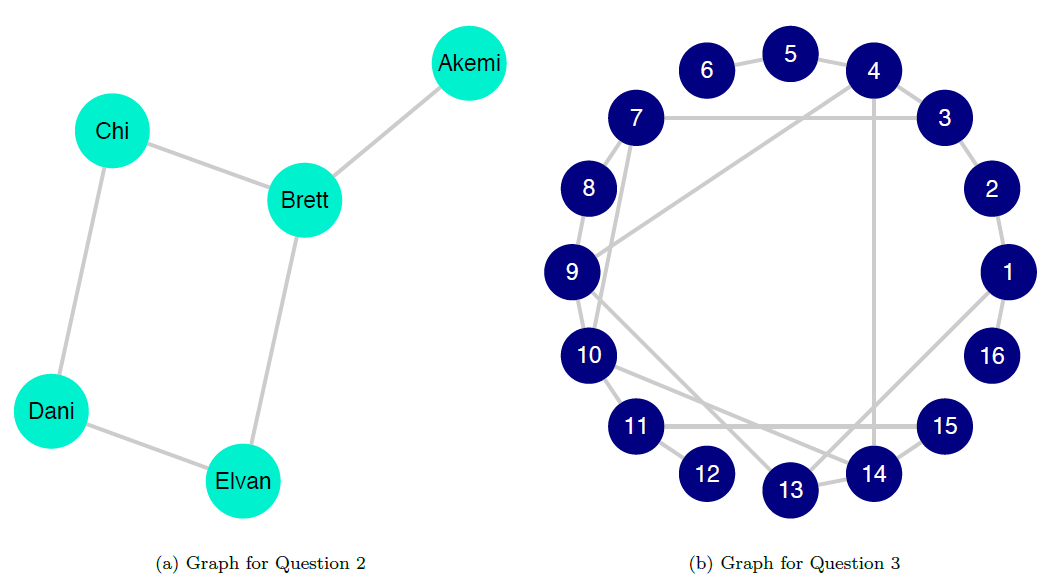
\includegraphics{images/social-networks/11-15.png}
\caption{Sociograms for Questions 2 (left) and 3 (right)}\label{fig:fig11-15}
}
\end{figure}

Social network analysis has the potential to refine our interpretations of
social relations and processes in the domain of political science. We can use
it to confirm or challenge hypotheses; we can sharpen or complicate how we
understand actors and relationships. By synthesizing established or
contentious knowledge with new insight, we can develop political theory,
thought, and practice---as well as advance political and social agendas.

\hypertarget{application-questions-8}{%
\section{Application Questions}\label{application-questions-8}}

\begin{enumerate}
\def\labelenumi{\arabic{enumi}.}
\item
  Which of the networks listed in {[}section 11.2.1{]} are examples of social
  networks?
\item
  Using the graph in figure @ref(fig:fig11-15), compute the following:

  \begin{enumerate}
  \def\labelenumii{\arabic{enumii}.}
  \item
    The betweenness centrality for Akemi and for Dani
  \item
    The closeness centrality for Brett and for Elvan
  \item
    The degree centrality for each node
  \item
    The network's density
  \end{enumerate}
\item
  Consider the graph in figure @ref(fig:fig11-15):

  \begin{enumerate}
  \def\labelenumii{\arabic{enumii}.}
  \item
    Is this an undirected or directed graph? How can you tell?
  \item
    Is this a weighted or unweighted graph? How can you tell?
  \item
    What is the minimum degree for this network? Which node or nodes have this
    degree?
  \item
    What is the maximum degree? Which node or nodes have this degree?
  \item
    Trace the geodesic between nodes \(1\) and \(7\). What is its length? What
    is this measure called?
  \item
    Is the network depicted most likely to be a geographic network, a
    small-world network, a power-law network, or a random network with
    \(p = .7\)?
  \end{enumerate}
\end{enumerate}

\hypertarget{key-terms-6}{%
\section{Key Terms}\label{key-terms-6}}

\begin{itemize}
\item
  adjacency matrix
\item
  betweenness centrality
\item
  centrality
\item
  closed triple
\item
  closeness centrality
\item
  complete graph
\item
  connected component
\item
  connected graph
\item
  degree centrality
\item
  degree distribution
\item
  diameter
\item
  directed graph
\item
  directed tie
\item
  disconnected graph
\item
  distance
\item
  dyad
\item
  edge
\item
  geographic network
\item
  indegree
\item
  isolate
\item
  local clustering coefficient
\item
  matrix
\item
  mean degree
\item
  mean path length
\item
  neighbors
\item
  network
\item
  network density
\item
  node
\item
  open triple
\item
  ordered triple
\item
  outdegree
\item
  path
\item
  path length
\item
  power-law network
\item
  random network
\item
  small-world network
\item
  social network
\item
  social network analysis
\item
  subgraph
\item
  tie
\item
  triad
\item
  triangle
\item
  triple
\item
  triplet
\item
  undirected graph
\item
  undirected tie
\item
  unweighted graph
\item
  vertex
\item
  weighted graph
\end{itemize}

\hypertarget{answers-to-application-questions-5}{%
\section{Answers to Application
Questions}\label{answers-to-application-questions-5}}

\begin{enumerate}
\def\labelenumi{\arabic{enumi}.}
\item
  The following are examples of social networks: The genealogical history of
  the Japanese royal family; email correspondence between workers in a
  corporation; mentorship and advising among political scientists in academia;
  and advice-seeking relationships among all current federal circuit judges in
  the United States
\item
  Using the graph in figure @ref(fig:fig11-5), we find the following:

  \begin{enumerate}
  \def\labelenumii{\arabic{enumii}.}
  \item
    Betweenness centrality:

    \begin{enumerate}
    \def\labelenumiii{\arabic{enumiii}.}
    \item
      Akemi: \(0\)
    \item
      Dani: \(0.5\)
    \end{enumerate}
  \item
    Closeness centrality:

    \begin{enumerate}
    \def\labelenumiii{\arabic{enumiii}.}
    \item
      Brett: \(0.2\)
    \item
      Elvan: \(0.167\)
    \end{enumerate}
  \item
    Degree centrality:

    \begin{enumerate}
    \def\labelenumiii{\arabic{enumiii}.}
    \item
      Akemi: \(1\)
    \item
      Brett: \(3\)
    \item
      Chi: \(2\)
    \item
      Dani: \(2\)
    \item
      Elvan: \(2\)
    \end{enumerate}
  \item
    Network density: \(0.5\)
  \end{enumerate}
\item
  Considering the graph in figure @ref(fig:fig11-15):

  \begin{enumerate}
  \def\labelenumii{\arabic{enumii}.}
  \item
    This is an undirected network. The edges do not have arrows to indicate
    asymmetric relationships, so they must be undirected.
  \item
    This graph is unweighted. There are no weights associated with any of the
    edges, so it must be unweighted.
  \item
    The minimum degree is \(1\) and nodes \(6\), \(12\), and \(16\) have a
    degree of \(1\).
  \item
    The maximum degree is \(4\) and nodes \(4\), \(9\), \(10\), and \(14\)
    have a degree of \(4\).
  \item
    See figure @ref(fig:11-16) for the highlighted path. The geodesic, or
    shortest path, between nodes \(1\) and \(7\) is \([1, 2, 3, 7]\) and has a
    path length of \(3\). This metric is called the \emph{geodesic distance}
    or simply the \emph{distance}.
  \item
    This network is most likely to be a small-world network because it has a
    large proportion of nodes with average degree centrality, and smaller
    proportions of nodes with low or high degree centrality. Furthermore: It
    can't be a geographic network because degree centrality varies by node. It
    is not likely to be a power-law network because it has several nodes of
    the maximum degree (also, it's unlikely that a graph with only sixteen
    nodes could follow a power-law distribution). It is not likely to be a
    random network with \(p = .7\) because that would imply that approximately
    \(70\%\) of pairs of nodes would be connected, which would, in turn, imply
    an average degree centrality of \(p \times N = .7 \times 16 = 10.5\); we
    know, however, that the mean degree is much lower than that as the maximum
    degree is \(4\).
  \end{enumerate}
\end{enumerate}

\begin{figure}
\hypertarget{fig:fig11-16}{%
\centering
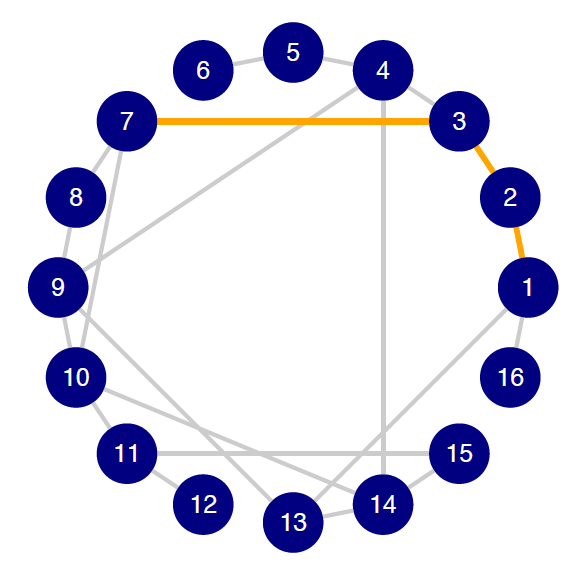
\includegraphics{images/social-networks/11-16.png}
\caption{Highlighted geodesic between 1 and 7}\label{fig:fig11-16}
}
\end{figure}

\hypertarget{machine-learning}{%
\chapter{Machine Learning}\label{machine-learning}}

\textbf{By John J. Lee}

\hypertarget{introduction-9}{%
\section{Introduction}\label{introduction-9}}

These days, references to machine learning are almost ubiquitous. If you
follow the news, you have probably heard that machine learning is used in a
wide range of contexts: e.g., to detect fraudulent transactions, predict stock
prices, perform facial recognition, customize search results, and even guide
self-driving cars. But what exactly is machine learning? Machine learning is
often conflated with related concepts including artificial intelligence,
automation, and statistical computing. Part of this confusion and ambiguity is
due to the reality that even among relevant experts in statistics and computer
science, there is no single ``correct'' definition of machine learning.
However, there are two well-known formal definitions. Both definitions were
cited by Andrew Ng (\protect\hyperlink{ref-ng-a}{Ng, n.d.}), in his highly
popular Stanford course on machine learning (available through
\href{https://www.coursera.org/learn/machine-learning}{Coursera}).

\begin{figure}
\hypertarget{fig:jl-figure1}{%
\centering
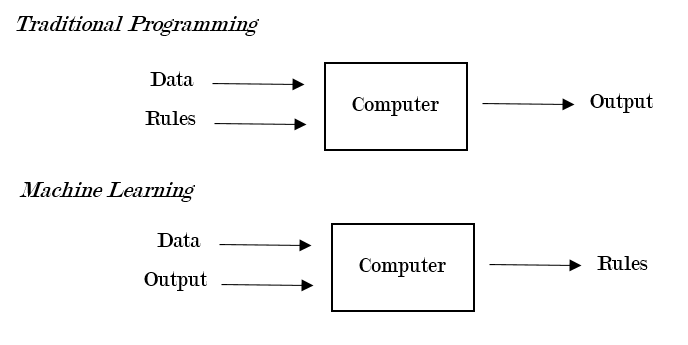
\includegraphics{images/ml/jl-figure1.png}
\caption{Traditional Programming v. Machine Learning}\label{fig:jl-figure1}
}
\end{figure}

The first definition is by Arthur Samuel, a former researcher at IBM and early
pioneer in machine learning. In his view, machine learning is a \emph{``field
of study that gives computers the ability to learn without being explicitly
programmed.''} This definition is useful because it alludes to a central
distinction between traditional programming and machine learning: i.e., in
traditional programming, a computer takes in the data and the rules and
generates the output; in machine learning, a computer takes the data and the
output and generates the rules that describe the relationship between the
input and the output. Figure @ref(fig:jl-figure1) provides an illustration of
this idea.

The second definition is more detailed and precise. According to Tom Mitchell,
a computer scientist at Carnegie Mellon and the author of one of the first
textbooks on machine learning: \emph{``A computer program is said to learn
from experience E with respect to some task T and some performance measure P,
if its performance on T, as measured by P, improves with experience E.''}
(\protect\hyperlink{ref-mitchell1997a}{Mitchell 1997}). From the second
definition, we can get a better sense of what machine learning generally
entails: i.e., a computer gradually becomes better at performing a specific
task (``what'') through experience (``how''); moreover, the computer's
performance is measured using some metric, which allows us to test whether
performance has indeed improved over time. In this chapter, I will provide an
overview of how machine learning methods work in practice and review some
examples of how political scientists have used these methods in their
research. Before proceeding, it is necessary to first explain several
fundamental concepts in machine learning (for a more detailed treatment of
this subject, see \protect\hyperlink{ref-hastie2017a}{Hastie, Tibshirani, and
Friedman 2017}; \protect\hyperlink{ref-james2013a}{James et al. 2013})

\hypertarget{background-3}{%
\section{Background}\label{background-3}}

\hypertarget{a-brief-note-on-notation}{%
\subsection{A Brief Note on Notation}\label{a-brief-note-on-notation}}

Capital letters refer to variables: e.g., \(Y\) refers to the outcome
variable, such as vote choice. Lower-case letters refer to the observed value
of the variable for a specific observation (or subject), denoted by the first
subscript: e.g., \(y_{1}\) refers to the value of the outcome variable for the
first observation. The subscript of a capital \(X\) refers to the number of
the predictor or explanatory variable: e.g., \(X_{1}\) refers to the first
predictor, \(X_{2}\) refers to the second predictor, and so on. In addition,
\(x_{ij}\) refers to the observed value of the \(j\)th predictor for the
\(i\)th observation. The \^{} symbol indicates that we are referring to the
predicted version or value of an object: e.g., \(\hat{f}(.)\) refers to an
estimated function, \(\hat{Y}\) refers to the predicted value of the outcome
variable.

\hypertarget{the-structure-of-prediction-error}{%
\subsection{The Structure of Prediction
Error}\label{the-structure-of-prediction-error}}

Machine learning practitioners often talk about the best ways to \("\)minimize
the mean squared error\("\) or \("\)optimize the bias-variance tradeoff.\("\)
To understand how machine learning works, it is very important to understand
the structure of prediction error. To illustrate, we can start with a simple
example of a regression type problem with a quantitative outcome. Let \(Y\) be
a 0-100 point feeling thermometer that measures attitudes toward the U.S.
president, with 0 being very unfavorable and 100 being very favorable. Assume
we are predicting \(Y\) using two predictors: ideology (\(X_{1}\)) and income
(\(X_{2}\)). Formally, we can represent the relationship between \(X_{1}\),
\(X_{2}\), and \(Y\) in the following way:

\[Y=f \left( X_{1}, X_{2} \right) + \epsilon\]

In the equation above, \({f}(.)\) is also known as the \textbf{target
function}, which represents the true systematic (i.e., non-random) part of the
relationship between the two predictors (\(X_{1}\), \(X_{2}\)) and the outcome
\(Y\). On the other hand, \(\epsilon\) is the random error term, which is
assumed to be independent of the predictors and have a mean of zero. In
reality, of course, we do not know \({f}(.)\), so we have to estimate it using
the data. Estimating the true function means that we are estimating the
model's parameters (e.g., the coefficients in a linear regression) or
structure (e.g., the shape of a regression tree). For example, suppose we have
a dataset (e.g., \(n\) observations) with the actual value of \(Y\),
\(X_{1}\), and \(X_{2}\) for each observation:
\(\{(y_{1},x_{11},x_{12}),...,(y_{n},x_{n1},x_{n2})\}\). Next, we will split
the dataset into at least two parts, so that we can estimate \({f}(.)\) using
one subset of the data (typically called the \textbf{training set}), and then
evaluate the prediction error using the second subset of the data (typically
called the \textbf{test set}).

Many machine learning algorithms are designed to estimate (or \("\)fit\("\)) a
model that minimizes the \textbf{expected} \textbf{prediction error (EPE)},
defined as the long-run \emph{average} difference between the predicted and
\("\)true\("\) (i.e., observed) values of the outcome variable. That is, the
goal is to identify \({f}(.)\) such that \(f(X_{1},X_{2})\) is on average as
close to \(Y\) as possible. How can we measure EPE in practice? When the
outcome is a quantitative variable, the algorithms are often designed to
minimize the mean squared error (MSE): i.e., the average of the squared
difference between \(\hat{Y}\) and \({Y}\). The intuition here is that when
the absolute difference between the predicted and observed values of the
outcome variable is generally small, MSE will also be small.

\[MSE=\frac{1}{n} \sum _{i=1}^{n} \left( y_{i}-\hat{f} \left( x_{i1},x_{i2} \right)  \right) ^{2}\]

Assuming we have split the original dataset into the training set and test
set, we can compute two different types of MSE: \textbf{training MSE} and
\textbf{test MSE}. In both cases, we first fit \(\hat{f}(.)\) using the
training set. The difference, which is fundamental to machine learning, is the
following: the training MSE (or training error, more generally) is then
computed using the data from the training set, which contains the same data
used to fit \(\hat{f}(.)\). In contrast, the test MSE (or test error) is
computed using the test set, which was not used to fit \(\hat{f}(.)\).

Recall that we randomly assigned the observations in the original full dataset
to the training and test sets. Thus, the two datasets are comparable: i.e.,
the true relationship between the set of predictors (\(X_{1}, X_{2}\)) and
\(Y\) should be the same in both datasets. However, the two datasets are also
not identical; these minor, non-systematic differences are due to random
noise, which are represented by the \(\epsilon\) in Eq. 1. Given this context,
it should be clear why we want to minimize test MSE instead of training MSE.

If we attempt to minimize training MSE, the algorithms are more likely to
estimate highly flexible models that try to touch every data point in the
feature space of the training dataset. This might initially sound nice, but it
means that the model is \textbf{overfitting} to the training set: i.e., the
model is attempting to capture both the real patterns due to the true
\({f}(.)\), as well as the observed but spurious deviations from \({f}(.)\)
that are due to the random noise (\(\epsilon\)). The problem here is that this
kind of highly flexible model tends to generate a lower training MSE, but
performs poorly on the test set---which has the same underlying patterns due
to \({f}(.)\), but different observed deviations from \({f}(.)\) because of
\(\epsilon\). Figure @ref(fig:jl-figure2) provides an illustration of this
idea. In this example, the true relationship between \(X_{1}\) and \(Y\) is
linear (see the graph in the middle); we know this for certain because these
data were simulated.

\begin{figure}
\hypertarget{fig:jl-figure2}{%
\centering
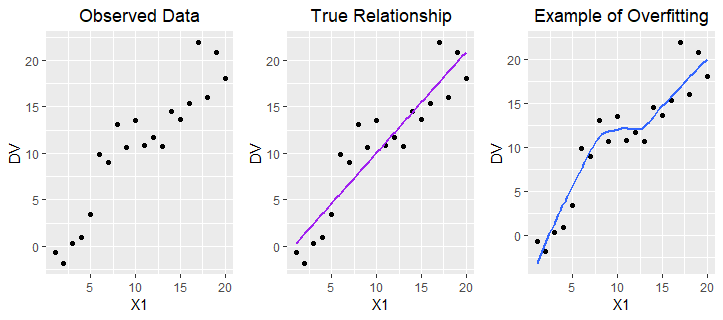
\includegraphics{images/ml/jl-figure2.png}
\caption{Modeling True Relationship v. Overfitting}\label{fig:jl-figure2}
}
\end{figure}

Thus, it is a better idea to try and minimize test error. In order to generate
a smaller test error, the algorithms need to estimate a model that is
generalizable. That is, they need to estimate models that do a better job of
capturing the true relationship between the set of predictors
(\(X_{1},X_{2}\)) and the \(Y\), while ignoring the random observed deviations
from the \({f}(.)\) due to \(\epsilon\) (per Equation 1). Machine learning
practitioners often refer to this approach as \("\)focusing on the signal and
ignoring the noise.\("\)

\textbf{Check-in Question 1:} What is overfitting and how can we reduce this
problem?

So how do we reduce the test error? The expected difference between
\(\hat{f}(X_{1},X_{2})\) and \(Y\) is due to two types of error (e.g., see
James et al.~2013): (1) \textbf{reducible error}, (2) \textbf{irreducible
error}. The first type of error is caused by a suboptimal estimate of the true
function: i.e., the gap between \(\hat{f}(.)\) and \(f(.)\). As its name
implies, the reducible error decreases as \(\hat{f}(.)\) approaches \(f(.)\).
On the other hand, irreducible error is due to \(\epsilon\), and therefore it
cannot be reduced by improving the quality of \(\hat{f}(.)\). For example, let
us assume that \(\hat{f}(.) = f(.)\), and therefore
\(\hat{Y} = \hat{f}( X_{1}+X_{2}) = f(X_{1}+X_{2})\). Even in this case,
\(\hat{Y}\) does not necessarily equal \(Y\), because
\(Y = f(X_{1}, X_{2}) + \epsilon\). That is, even having a perfect estimate of
\(f(.)\) does not make the random error term go away.

Can we reduce \(\epsilon\)? The random error term represents omitted variables
as well as truly random noise. If there are variables that are both useful
predictors of \(Y\) and also largely independent of the existing predictors
(\(X_{1},X_{2}\)), then by adding them into the model we can reduce
\(\epsilon\). On the other hand, some of the \(\epsilon\) is ultimately due to
random noise, and this component of \(\epsilon\) cannot be eliminated: e.g.,
perhaps some of the subjects felt particularly well/poorly the day they were
surveyed, which affected how they responded to the survey questions.

To formally decompose the expected test error into its reducible and
irreducible components, we can use the \textbf{expected value} (or long-run
average) of the squared difference between \(\hat{Y}\) and \(Y\).\footnote{Here
  is a more detailed explanation of what is meant by this sentence. The
  squared difference between \(Y\) and \(\hat{Y}\) is actually a continuous
  random variable. In statistical theory, a random variable is a variable
  whose value is the outcome of a random process. Recall that in the general
  case \(Y = f(X) + \epsilon\), where \(X\) represents a set of predictors.
  Since \(Y\) is the function of the random error component \(\epsilon\),
  \(Y\) is by definition a random variable. Now, notice that since
  \((Y-\hat{Y})^{2}\) is a function of the random variable \(Y\),
  \((Y-\hat{Y})^{2}\) must also be a random variable. In particular,
  \((Y-\hat{Y})^{2}\) is a continuous random variable, since it can
  theoretical take on an infinite number of possible (non-negative) values. We
  can think of the expected value of a random variable as being the weighted
  or ``long-run'' average of the random variable's possible values. To
  simplify the notation, let \(W=(Y-\hat{Y})^{2}\). Formally, let's assume
  that the random variable \(W\) has a probability density function \(g(w)\),
  which determines the distribution of the probabilities associated with the
  possible values of \(W\). The lower-case \(w\) represents specific possible
  values of the random variable \(W\). In this case, then
  \(E(W) = \int_{-\infty}^{\infty} wg(w) dw\).} The following proof requires
knowledge of statistical theory (Larsen and Marx 2017; Rice 2007) and some
basic algebra. To simplify the notation, let \(X=X_{1}+X_{2}\).

\[E \left[  \left( Y-\hat{Y} \right) ^{2} \right] =E \left[  \left( f \left( X \right) + \epsilon -\hat{f} \left( X \right)  \right) ^{2} \right]\]

\[=E \left[  \left(  \left( f \left( X \right) -\hat{f} \left( X \right)  \right) + \epsilon  \right) ^{2} \right]\]

\[=E \left[  \left( f \left( X \right) -\hat{f} \left( X \right)  \right) ^{2}+2 \epsilon  \left( f \left( X \right) -\hat{f} \left( X \right)  \right) + \epsilon ^{2} \right]\]

\[=E \left[  \left( f \left( X \right) -\hat{f} \left( X \right)  \right) ^{2} \right] +E \left[ 2 \epsilon  \left( f \left( X \right) -\hat{f} \left( X \right)  \right)  \right] +E \left(  \epsilon ^{2} \right)\]

\[=E \left[  \left( f \left( X \right) -\hat{f} \left( X \right)  \right) ^{2} \right] +Var \left(  \epsilon  \right)\]

The first term, or the expected squared difference between \(\hat{f}(X)\) and
\({f}(X)\), represents the reducible error. The second term,
\(Var(\epsilon)\), represents the irreducible error. Although a full proof is
beyond the scope of this chapter, note that we can further decompose the
reducible error into squared \textbf{bias} and \textbf{variance}.

\[E \left[  \left( f \left( X \right) -\hat{f} \left( X \right)  \right) ^{2} \right] = \left[ E \left( \hat{f} \left( X \right)  \right) -f \left( X \right)  \right] ^{2}+E \left[  \left( \hat{f} \left( X \right) -E \left( \hat{f} \left( X \right)  \right)  \right) ^{2} \right]\]

\[= \left[ Bias \left( \hat{f} \left( X \right)  \right)  \right] ^{2}+Var \left( \hat{f} \left( X \right)  \right)\]

In sum, the expected test error (or expected prediction error, EPE) is a
function of three specific quantities: the bias of \(\hat{f}(X)\), which
indicates the gap between \(\hat{f}(.)\) and \(f(.)\); the variance of
\(\hat{f}(X)\), which indicates how much \(\hat{f}(.)\) fluctuates depending
on the training data; and \(Var(\epsilon)\), which is a measure of the
non-systematic random noise in the data.

\[EPE=E \left[  \left( Y-\hat{Y} \right) ^{2} \right] = \left[ Bias \left( \hat{f} \left( X \right)  \right)  \right] ^{2}+Var \left( \hat{f} \left( X \right)  \right) +Var \left(  \epsilon  \right)\]

The key insight is that the reducible error is itself a function of the
squared bias and variance of \(\hat{f}(.)\), or the estimated model. Thus, to
minimize the reducible error (and hence the total EPE), we want to minimize
the bias and the variance.

\textbf{Check-in Question 2:} What is the expected prediction error (EPE), and
why does it matter?

\hypertarget{bias-variance-trade-offs}{%
\subsection{Bias-Variance Trade-offs}\label{bias-variance-trade-offs}}

In machine learning, \textbf{bias} is a measure of the size of the gap between
\(\hat{f}(.)\) and \({f}(.)\).\footnote{Another way to think about bias is
  that it is the systematic part of the difference between \(Y\) and
  \(\hat{Y}\). When \(\hat{f}(.)\neq{f}(.)\), the observed difference between
  \(Y\) and \(\hat{Y}\) is often correlated with the gap between the estimated
  function and the true function.} The bias is smaller when the model does a
better job of representing the true relationship between the set of predictors
\((X_{1},X_{2},...,X_{p})\) and \(Y\). For example, let's assume that the true
relationship between \(X_{2}\) and \(Y\) is described using an inverted
U-shaped curve. If the model we select imposes a linear functional form, then
the bias will be larger than if the model allowed nonlinearity. Thus, to
reduce bias, we often want to use a more flexible model.

However, it is possible for the model to be too flexible. \textbf{Variance} is
a measure of the stability or consistency of the estimated model across
training sets. If small changes to the training set (e.g., dropping a few
observations) causes large changes in \(\hat{f}(.)\), then the variance is
high. A highly flexible model tends to reduce bias but also increase variance
(hence the idea of a \("\)trade-off\("\)). Thus, the goal is to fit a model
that is flexible enough to capture the true relationship between the set of
predictors \((X_{1},X_{2},...,X_{p})\) and \(Y\), but not so flexible that it
is also fitting to the observed deviations from \({f}(.)\) in the training set
due to \(\epsilon\).

\begin{figure}
\hypertarget{fig:jl-figure3}{%
\centering
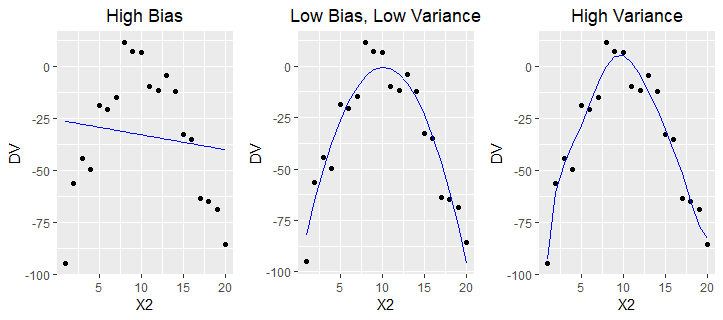
\includegraphics{images/ml/jl-figure3.png}
\caption{Bias-Variance Trade-offs}\label{fig:jl-figure3}
}
\end{figure}

Figure @ref(fig:jl-figure3) provides an illustration of this idea. The first
model is not flexible enough, leading to high bias (also known as
\textbf{underfitting}); on the other hand, the third model is too flexible,
which leads to higher variance across slightly different training sets
(\textbf{overfitting}). The second model imposes the ideal amount of
flexibility, which optimizes the bias-variance trade-off and yields the
smallest test MSE of the three alternatives.

\textbf{Check-in Question 3:} Explain why reducing bias can often entail an
increase in variance.

\hypertarget{parametric-v.-non-parametric-methods}{%
\subsection{Parametric v. Non-parametric
Methods}\label{parametric-v.-non-parametric-methods}}

Machine learning algorithms that make explicit assumptions about the
functional form of the relationship between the set of predictors and \(Y\)
are known as \textbf{parametric methods}. A well-known example is the ordinary
least squares (OLS) regression. Given two predictors,
\(f \left( X_{1}, X_{2} \right) = \beta _{0}+ \beta _{1}X_{1}+ \beta _{2}X_{2}\).
Thus, the regression equation in this case can be written as follows:

\[Y= \beta _{0}+ \beta _{1}X_{1}+  \beta _{2}X_{2}+ \epsilon\]

Parametric methods offer several key advantages. First, they simplify the task
of estimating \(f(.)\) by making an assumption about the functional form or
shape of \(f(.)\). In the case of an OLS regression, the algorithm assumes
that \(f(.)\) is linear with respect to the parameters (i.e., the coefficients
and the error term), although not necessarily with respect to the values of
the predictors. Thus, the only task is to estimate coefficients:
\(\beta _{0}, \beta _{1}, ..., \beta _{p}\). Second, because of the functional
form assumption, the \(\hat{f}(.)\) tends to be more stable across comparable
training sets (i.e., lower variance); put differently, the estimated model is
more robust to minor fluctuations due to \(\epsilon\). Another advantage is
that parametric methods also tend to score high on \textbf{interpretability}:
e.g., we can easily interpret \(\beta _{1}\) as indicating that a one-unit
change in \(X_{1}\) is associated with a change of \(\beta _{1}\) in \(Y\).
Other examples of parametric methods include logistic regression, penalized
regression methods (e.g., lasso, ridge), and linear discriminant analysis. The
main disadvantage of parametric methods is the risk of imposing a functional
form that is very different from the true \(f(.)\), which can result in higher
bias (or more prediction error). We can mitigate this risk by adjusting the
parametric methods so that they are more flexible (e.g., by using higher-order
terms in an OLS regression), but this may come at the cost of higher variance.

Non-parametric methods do not assume that the true relationship between a set
of predictors and \(Y\) follows a specific functional form; instead, they
inductively attempt to estimate \(f(.)\) such that it closely follows the
training observations in the feature space. Well-known examples of
non-parametric methods include tree-based methods (e.g., random forests,
boosted trees), support vector machines (SVM), and K-nearest neighbor (KNN).
The main advantage of non-parametric methods is that by design, they are very
flexible; this means that they can be particularly useful when the
relationship between the predictors and the outcome is highly complex. In such
cases, non-parametric methods can outperform parametric methods by achieving
lower bias, and ultimately, lower test error.

However, non-parametric methods also have a number of disadvantages. Since
they do not make assumptions about the functional form, they often require
much larger training sets in order to estimate \(f(.)\). In addition, because
they are highly flexible, non-parametric methods may also be subject to higher
variance across training sets due to overfitting. This can be mitigated by
properly tuning the models using \textbf{cross-validation (CV)}, a model
selection procedure discussed later in this chapter. Finally, it is also often
more difficult to interpret the nature of the relationship between a specific
predictor (e.g., \(X_{1}\)) and the outcome. This is why some especially
complex non-parametric methods such as artificial neural networks (ANN) are
often called \("\)black box algorithms,\("\) since it is not clear exactly how
the \(f(.)\) is being estimated.

Given this discussion, which methods are preferred? It depends on the size of
the available data, the complexity of the relationships among the variables,
and the goals of the method. Machine learning practitioners are often
interested in \textbf{prediction} or \textbf{(causal) inference}. If the goal
is prediction, then we are less concerned about understanding the specific
nature of \(f(.)\). Instead, we are satisfied as long as we can estimate a
model such that \(\hat{f}(X) \approx Y\). In this case, we should choose the
parametric or non-parametric method that generates the lowest expected test
error. On the other hand, if we are interested in understanding the specific
nature of the relationship between a given predictor (or group of predictors)
and the outcome, it may make more sense to select a parametric method, which
produces results (e.g., regression coefficients) that are easier to interpret.
While social scientists are often more interested in causal inference than
prediction alone, they have used both parametric and non-parametric methods in
their research. Several examples from political science will be discussed
later in this chapter.

\hypertarget{supervised-v.-unsupervised-learning}{%
\subsection{Supervised v. Unsupervised
Learning}\label{supervised-v.-unsupervised-learning}}

We can also classify machine learning methods according to whether they
predict a specific outcome. In \textbf{supervised learning}, there is a
clearly defined \("\)correct answer\("\) -- and the purpose of the machine
learning algorithm is to correctly predict that answer. For instance, let us
assume we want to predict whether a U.S. citizen will vote in the next
presidential election. This is an example of a supervised learning problem;
since the person either will or will not vote, there is clearly a \("\)correct
answer.\("\) There are two types of supervised learning, which are
distinguished by the type of outcome predicted: (1) \textbf{regression}, (2)
\textbf{classification}. In regression, the goal is to predict a continuous or
quantitative outcome: e.g., test scores, stock prices, inflation rates, number
of children, and so on.\footnote{Examples of popular supervised learning
  methods for regression include the ordinary least squares (OLS) regression,
  penalized/shrinkage methods such as the ridge and lasso regressions,
  regression trees, and artificial neural networks (ANN).} In classification,
the goal is to predict a categorical or discrete outcome: e.g., religion,
political party membership, vote choice, occupation, whether a person holds a
four-year degree.\footnote{Examples of popular supervised learning methods for
  classification include various implementations of the logistic regression
  (i.e., binary, ordinal, multinomial), k-nearest neighbor (KNN), linear
  discriminant analysis (LDA), quadratic discriminant analysis (QDA), support
  vector classifiers (SVC), support vector machines (SVM), classification
  trees, and artificial neural networks (ANNs).}

In \textbf{unsupervised learning}, the purpose of the machine learning
algorithm is to examine the underlying structure of the data and identify
\("\)hidden\("\) patterns. It is not attempting to correctly predict an
outcome. One well-known example of an unsupervised learning method is
clustering: clustering algorithms (e.g., hierarchical, k-means) identify
latent groups of observations by examining the relationships among the
variables associated with the observations (Bryan 2004; Wagstaff and Cardie
2000; Witten 2011). In this case, we do not know ahead of time what the
\("\)correct\("\) or \("\)true\("\) number of clusters is. Researchers can use
clustering algorithms to identify more internally homogeneous groups of
subjects (e.g., with respect to demographic characteristics, attitudes,
preferences, consumption patterns). Figure @ref(fig:jl-figure4) provides an
illustration of how we may organize machine learning methods by type and
subtype. Please note that the list of examples is not meant to be exhaustive.

\begin{figure}
\hypertarget{fig:jl-figure4}{%
\centering
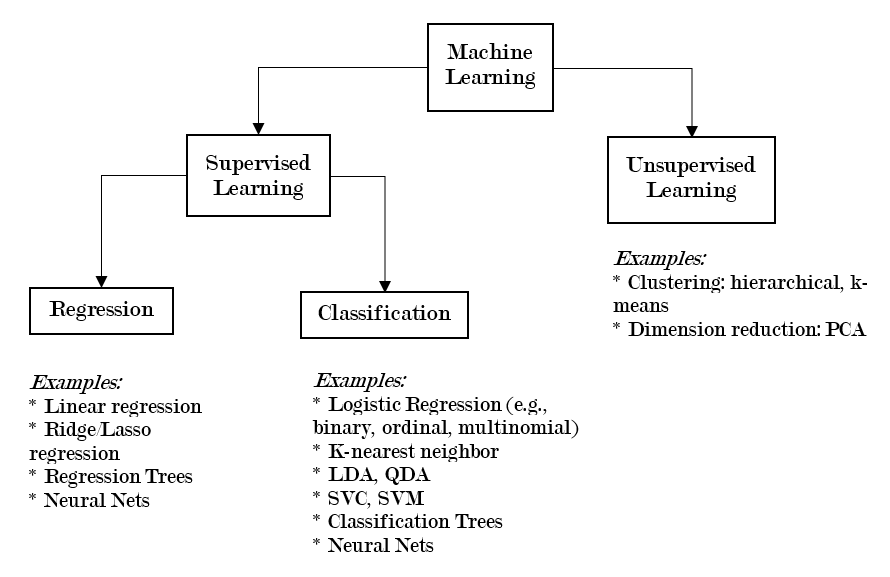
\includegraphics{images/ml/jl-figure4.png}
\caption{Types of Machine Learning Methods}\label{fig:jl-figure4}
}
\end{figure}

\textbf{Check-in Question 4:} What is the main difference between supervised
and unsupervised learning?

\hypertarget{method-setupoverview-3}{%
\section{Method: setup/overview}\label{method-setupoverview-3}}

There are definitely variations in how researchers and other practitioners
organize their machine learning projects. However, the workflow tends to
follow a general pattern. Assuming you already decided to use one specific
method (e.g., lasso regression), the workflow may look something like this:

\begin{enumerate}
\def\labelenumi{\arabic{enumi}.}
\item
  Split the data into training and test sets
\item
  With just the training set, use k-fold cross-validation (CV) to perform
  \textbf{model selection} (i.e., optimize the tuning parameters)
\item
  Fit the final optimized version of the model (also called the
  \textbf{candidate model}) using the full training set
\item
  Assess the candidate model by computing the test error
\end{enumerate}

If you would like to compare the performance of multiple methods (e.g.,
boosted trees, random forests), then only a few modifications to the sample
workflow above are necessary. Repeat steps 2-4 for each of the methods. At the
final stage, you will have the test error for each candidate model: depending
on your ideal trade-off between accuracy and interpretability, you can then
select the most preferred model. For example, if the goal is causal inference,
then you may be willing to select the candidate model with a somewhat higher
test error because it scores much higher on interpretability.

\hypertarget{what-is-model-selection}{%
\subsection{What is Model Selection?}\label{what-is-model-selection}}

The performance of machine learning models is often highly dependent on their
\textbf{tuning parameters}. We can think of tuning parameters as levers of the
model that allow us to customize or adjust how it operates. \textbf{Model
selection} refers to the process of identifying the tuning parameters that
yield the lowest expected test error; this is also referred to as
\("\)optimizing the tuning parameters.\("\) For example, consider the lasso
regression, which is a powerful method when we know that most of the
predictors are probably not useful for predicting the outcome. If a normal OLS
regression is used in this situation, the coefficients that should actually be
zero may remain at non-zero values---which increases the likelihood of the
model overfitting to the training data.

The algorithms for the OLS and lasso regressions are similar, except that the
optimization process for the latter is subject to an additional constraint.
Basically, this extra constraint imposes a penalty for the sum of the
coefficients for the \(p\) predictors in the model. The size of the penalty is
controlled by \(\lambda\): the bigger the \(\lambda\), the smaller the
coefficients. In fact, when the \(\lambda\) is sufficiently large, many of the
coefficients are totally zeroed out, which means that the lasso regression
also provides a means of automating the variable selection process. Next, I
explain why we typically use a method known as \(k\)-fold cross-validation to
perform the model selection procedure.

\[\lambda  \sum _{j=1}^{p} \vert  \beta _{j} \vert\]

\hypertarget{why-k-fold-cross-validation}{%
\subsection{Why K-Fold Cross-Validation?}\label{why-k-fold-cross-validation}}

For example, let us assume that we want to compare 100 unique values of
\(\lambda _{i}\) for the lasso regression; how do we know which value will
yield the lowest test error rate?

One option is using the \textbf{validation set approach}. This entails
randomly splitting the training set (\(n_{1}\)) into two non-overlapping
subsets: a model-building set (\(n_{1a}\)) and a validation set (\(n_{1b}\)).
Next, we fit a model using the model-building set (\(n_{1a}\)) and the first
value of lambda (\(\lambda _{1}\)), and then test it against the validation
set (\(n_{1b}\)). We would then repeat this process 99 more times, so that we
have done it once for each \(\lambda _{i}\). Afterward, we could compare the
100 validation error rates and identify the value of the parameter that
generated the lowest validation error. However, this approach has two
important disadvantages (\protect\hyperlink{ref-james2013a}{James et al. 2013,
176--78}). First, the estimated validation error rate for each
\(\lambda _{i}\) is highly variable, since it is very sensitive to the
specific observations that were randomly selected to be in \(n_{1a}\) and
\(n_{1b}\); if a small percentage of the observations in the \(n_{1a}\) were
moved to \(n_{1b}\) (and vice-versa), the test error rate would likely change.
Second, statistical learning models tend to perform more poorly when trained
on a smaller dataset; thus, by only training the model on a subset of the full
training set (i.e., since \(n_{1a} \ll n_{1}\) ), we may actually overestimate
the test error.

\(K\)-fold cross-validation (CV) is a statistically efficient resampling
method that addresses both of these problems. The purpose of CV is to provide
a more reliable estimate of the test error, which can then be used to compare
and evaluate unique values of the tuning parameters (e.g., \(\lambda _{i}\)).
It involves randomly splitting the training set (\(n_{1}\)) into \(k\)
non-overlapping groups (or \("\)folds\("\)) that are equal in size; the first
fold is treated as the held-out validation set, and the model is fit using the
observations in the remaining \(k-1\) folds. This process is repeated until
each fold has served as a validation set.

If there are 10 folds, there are also 10 estimates of the validation error;
these estimates are averaged to form the CV error rate. The idea is that this
CV error rate is a more reliable estimate of the validation error since it is
based on an average of \(k\) estimates (i.e., the CV error rate has a lower
variance). Returning to the previous example, if we wanted to test 100
potential values of \(\lambda _{i}\), we would perform the \(k\)-fold CV
procedure for each \(\lambda _{i}\); then, we would choose the value of
\(\lambda _{i}\) that yielded the lowest CV error.

\hypertarget{method-detail-1}{%
\section{Method: detail}\label{method-detail-1}}

In this section, I provide a brief overview of two common classes of machine
learning methods, and how they actually work in practice: (1) tree-based
methods, (2) support vector machines. Since we have used quantitative outcomes
so far in our examples, this time the examples will focus on classification: 1
= voted for Trump in 2016, 0 = voted for someone else.

\hypertarget{model-class-tree-based-methods}{%
\subsection{Model Class: Tree-based
Methods}\label{model-class-tree-based-methods}}

All tree-based methods (e.g., bagged trees, random forests, boosted trees)
share some important similarities. Each tree divides the training observations
into \(m\) non-overlapping regions of the predictor space
\(\{ R_{1},R_{2}, \ldots R_{m} \}\). Internal nodes refer to the place where
the splits are made. The algorithm uses binary recursive splitting, and
generally operates in the following way. The splits (i.e., predictor used,
values of the predictor) are chosen in order to maximize the purity or
homogeneity of the child nodes with respect to outcome class: i.e., in this
case, whether or not the respondents voted for Trump (i.e., \(Vote=1\) or
\(Vote=0\)). As such, the first split has the most explanatory power (i.e., in
terms of being able to predict the outcome class of a training observation),
the second split has the second most explanatory power, and so on.

Node purity or homogeneity is often measured using the Gini index or entropy.
In both cases, the measures are smaller when the nodes (or regions) are more
homogeneous; thus, the objective is actually to choose splits that minimize
the Gini index or entropy (which is equivalent to maximizing node purity). The
Gini index is defined below (\protect\hyperlink{ref-james2013a}{James et al.
2013, 312}). Here, \(p_{mk}\) represents the proportion of the training
observations that are in \(m\)th region (\(R_{m}\)) from the \(k\)th class.
Recall that \(G\) is small when the nodes are more homogeneous: e.g., when the
proportion of training observations in \(m\)th region are closely split
between two classes \(45\% -55\%\), then \(G = (.45)(.55)(2) =0.495\); in
contrast, when the training observations in \(R_{m}\) are more dominated by a
single class (and thus \(R_{m}\) is more homogeneous), for instance,
\(90\% -10\%\) , then \(G = (.10)(.90)(2) = 0.18\).

\[G= \sum _{k=1}^{K}p_{mk} \left( 1-p_{mk} \right)\]

How does this work in practice? For example, let us assume that in the
training set, being white v. not being white was the strongest individual
predictor of the Trump vote (i.e., it would maximize node purity). If this
were the case, then the first split would be based on race: all white
respondents would be assigned to the right branch, and all non-white
respondents would be assigned to the left branch (see Figure
@ref(fig:jl-figure5) below). Next, let us assume that among white respondents,
being above the mean on the 1-7 point political conservatism scale is the
strongest predictor of the Trump vote; if so, then the second split would be
based on whether the white respondents' conservatism score is \(\leq 4.3\)
(left branch) or \(> 4.3\) (right branch).

\begin{figure}
\hypertarget{fig:jl-figure5}{%
\centering
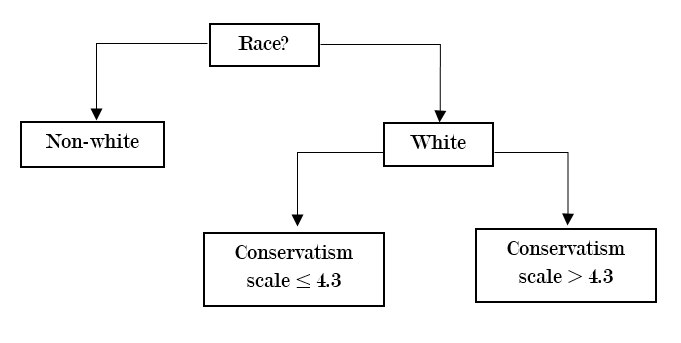
\includegraphics{images/ml/jl-figure5.png}
\caption{Example of a Decision Tree}\label{fig:jl-figure5}
}
\end{figure}

In this simple example, the observations (or respondents) in the training set
are assigned to one of three non-overlapping regions in the predictor space:
\({R_{1}= \{Vote \vert minority}\}\),
\(R_{2} = \{Vote \vert white, conservatism \leq 4.3\}\), and
\(R_{3}= \{Vote \vert white, conservatism > 4.3 \}\). To predict the outcome
class of an observation in the validation or test set, we simply look at which
region the observation would be assigned to based on its predictor values
(e.g., is \(x_{1} = white\)?), and then choose the most common class of that
region. For instance, if the test observation would belong to \(R_{3}\), and
\(70\%\) of the training observations in \(R_{3}\) voted for Trump, then the
predicted class of that test observation would be \(Vote=1\). In general, of
course, there are usually more than three regions (or terminal nodes); the
splitting ends once a stopping point is reached: e.g., in order to satisfy the
minimum terminal node size.

Individual decision trees suffer from high variance: i.e., the structure of
the tree is highly dependent on which specific observations randomly end up in
the training set. To address this issue, we can use the average prediction of
many different trees. Methods for combining these different trees are called
decision tree ensembles. There are three popular approaches:
bagging\footnote{This entails creating \(B\) bootstrap samples by sampling
  with replacement from the original training set (\(n_{1}\)). A
  classification tree is fit using each sample, and then the trees are
  combined (Cutler et al.~2014). This method is superior to using a single
  decision tree, because a single decision tree is affected by high variance;
  in contrast, by averaging the predictions across many \(B\) trees, the
  variance is reduced. The main tuning parameter for bagged trees is \(B\),
  the number of bootstrapped trees.}, random forests\footnote{This is the same
  as bagging, but now the model is only allowed to consider only a random
  subset \(m\) of the \(p\) predictors at each split (such that \(m \ll p\),
  e.g., \(n \approx \sqrt{p}\)). The logic here is that by intentionally
  restricting the number of predictors that can be considered at each split,
  the trees will become less correlated (Cutler 2005). In many cases,
  decorrelating the \(B\) trees in this way can lead to reduced test error.},
and boosting\footnote{With boosted trees, the trees are grown sequentially:
  each tree is fit to the residuals from the previous model. The logic of this
  approach is that it allows each successive tree to address the weaknesses of
  the previous tree.}

\hypertarget{model-class-support-vector-machines}{%
\subsection{Model Class: Support Vector
Machines}\label{model-class-support-vector-machines}}

Support Vector Machines (SVMs) are a class of methods that seek to assign
observations to the correct outcome by using hyperplanes as decision
boundaries. Hyperplanes are a \(p-1\) dimensional flat subspace in a
\(p\)-dimensional space: e.g., if \(p = 2\) (there are 2 predictors), then the
hyperplane is simply a line. For instance, let us assume a simple case in
which we are predicting the binary outcome \(Vote\) using only two predictors;
in this case, the separating hyperplane is a line. If the respondents in the
training set who voted for Trump are labeled as \(y_{i}=1\), and those who did
not vote for Trump are labeled as \(y_{i}=-1\), then the separating hyperplane
can be formally described as follows:

\[y_{i} \left(  \beta _{0}+ \beta _{1}x_{i1}+ \beta _{2}x_{i2} \right) >0\]

In this case, when \(\beta _{0}+ \beta _{1}x_{i1}+ \beta _{2}x_{i2}>0\),
\(y_{i}=1\) and if \(\beta _{0}+ \beta _{1}x_{i1}+ \beta _{2}x_{i2}<0\), then
\(y_{i}=-1\). That is, we can classify the observations based on whether they
are above or below the separating hyperplane.

Next, I will briefly review how SVMs have been designed to address two key
practical challenges. The first challenge is that there are often many
hyperplanes that can correctly classify the observations, since the hyperplane
can be slightly adjusted in any direction and probably still produce the same
classifications. If we return to the equation above, it is easy to see that
there are many ways the coefficients \(\beta {0}\), \(\beta {1}\), and
\(\beta {2}\) can be slightly adjusted (e.g., a \(0.5\%\) increase or
decrease) and still perfectly classify the observations. The solution is to
maximize the margins, or the distance between the training data points and the
separating hyperplane: this is also known as the maximal margin classifier or
MMC.

Unfortunately, the MMC approach faces its own problems. Sometimes, there is
simply no perfectly separating hyperplane; and even if there is, it is highly
sensitive to individual observations, which can lead to overfitting (and high
variance). The solution is a more flexible form of the MMC that allows some
observations to fall on the wrong side of the margin and/or hyperplane: this
is also known as the support vector classifier (SVC). The SVC is more robust
in that it is less sensitive to individual observations, such as outliers
(i.e., since some violations of the margin are allowed); this property allows
the SVC to do a better job of classifying the observations in \emph{general}.

Like the MMC, the SVC seeks to maximize the margin, but it is subject to a
number of important constraints (\protect\hyperlink{ref-james2013a}{James et
al. 2013, 346--47}). Here, I will specifically focus on the cost parameter
(\(C\)), since that is what is generally optimized using cross-validation.
Below, \(\epsilon {i}\) indicates how severely the \(i\)th observation
violates the margin and separating hyperplane. When \(\epsilon {i}=0\), the
\(i\)th observation is located on the correct side of the margin (i.e., no
error); when \(\epsilon {i}>0\), it is on the wrong side of the margin; and if
\(\epsilon {i}>1\), it has actually violated the separating hyperplane. That
is, \(C\) essentially represents the budget for the number and severity of the
classification errors across the \(n\) observations. When \(C\) is small, the
SVC will fit more tightly to the training observations in the feature space,
at the cost of higher variance; and when \(C\) is large, the opposite can
occur. To optimize this bias-variance trade-off, we can use k-fold CV.

\[\sum {i=1}^{n} \epsilon {i} \leq C\]

The SVM is an extension of the SVC, which allows us to model nonlinear
decision boundaries using kernels. By using kernels, the SVM allows us to
expand the feature space (e.g., include polynomial functions of the
predictors) in a computationally efficient manner. For more details on this
procedure, we can refer to James et al.~2013, pp.~350-353; and Hastie et
al.~2017, pp.~423-426).

\hypertarget{applications-4}{%
\section{Applications}\label{applications-4}}

In this section, I review six recent examples of machine learning methods in
political science articles. The examples cover applications of both supervised
learning (e.g., RF, SVM, naïve Bayes, k-nearest neighbor); and unsupervised
methods such as topic modeling, which is related to clustering. Several
different subfields of political science are represented: U.S. politics,
political theory, comparative politics, international relations, and peace and
conflict studies; in addition, the articles use data from many countries
around the world (e.g., Argentina, India).

\hypertarget{example-1-u.s.-politics}{%
\subsection{Example 1: U.S. Politics}\label{example-1-u.s.-politics}}

DW-NOMINATE scores are often used in political science as a measure of a
legislator's ideology; they are based on the actual votes the legislators have
made on bills in the U.S. House or U.S. Senate. uses two supervised machine
learning methods (i.e., support vector regression and random forests) to
address a very interesting problem: how can we predict the ideology of new
legislators before they begin casting their votes? Support vector regression
(SVR) is very similar to SVM, except that the algorithm has been modified to
enable the prediction of a continuous outcome. In the first part of the paper,
the author uses 10-fold CV to train models that predict the candidates'
DW-NOMINATE scores based on their campaign contributions, gender, party, and
home state. The training set includes candidates with DW-NOMINATE scores
between 1980-2014; and the key predictors in the feature matrix are the names
of donors who have given to at least 15 candidates (e.g., National Education
Association).

According to the results (i.e., RMSE),\footnote{Root mean squared error (RMSE)
  is a measure of the average absolute difference between the predicted value
  of the outcome and the actual observed value. The smaller the RMSE, the more
  accurate the estimates of the outcome.} the support vector regression and
random forest methods perform at least as well as the other methods that
actually use the roll call data. This is especially impressive when we
consider that the roll call data are used to construct the DW-NOMINATE scores.
Next, Bonica also shows that the supervised learning methods also do a very
good job of correctly predicting the actual votes cast during the
96\textsuperscript{th}-113th Congresses: e.g., 89.9\(\%\) of the votes are
correctly predicted using DW-NOMINATE, which is not surprising; however,
89.5\(\%\) and 89.3\(\%\) of the votes are also correctly classified using the
RF and SVR methods that were only trained using campaign contributions and a
few other predictors.

\hypertarget{example-2-comparative-politics}{%
\subsection{Example 2: Comparative
Politics}\label{example-2-comparative-politics}}

How do we know whether an election was rigged? Using synthetic (i.e.,
simulated) data, Cantú and Saiegh (\protect\hyperlink{ref-cant2011a}{2011})
train a naïve Bayes classifier that successfully identifies fraudulent
elections in the Buenos Aires province of Argentina between 1931 and 1941. One
of the greatest strengths of the naïve Bayes (NB) algorithm is its simplicity,
which is due the assumption that the features (i.e., predictors) are
independent.\footnote{Although this is a strong assumption, research has shown
  that NB algorithm is robust to minor deviations from independence of the
  features.} For every election, the algorithm first estimates the posterior
probability of membership in each class (i.e., fraudulent or clean) given the
set of observed features or attributes associated with the election. The
predicted class of each election is the class with the largest posterior
probability, per Bayes theorem. For example, given a set of features, if the
election is even slightly more likely to be fraudulent than clean, the
election is classified by NB as a fraudulent election, and vice versa. After
training their NB classifier on a large synthetic dataset (N=10,000), the
authors test their model using several well-documented elections in 1936,
1940, and 1941; they show that their method ultimately outperforms key
existing fraud detection algorithms (e.g., those based on the distributions of
digits in official vote counts).

\hypertarget{example-3-political-theory}{%
\subsection{Example 3: Political Theory}\label{example-3-political-theory}}

Can machine learning be used to study the evolution of political theory across
centuries? During the medieval and early modern period, scholars and other
elites often wrote advice books for leaders that covered topics such as
military strategy, economic prosperity, and religious devotion. These books
provide an insightful view or \("\)mirror\("\) into the dominant political
theories and paradigms of the day. Blaydes, Grimmer, and McQueen
(\protect\hyperlink{ref-blaydes2018a}{2018}) use automated text analysis to
compare how political advice texts in the Medieval Christian and Islamic
Worlds changed during the medieval period. Their corpus of text includes 21
texts from the medieval Islamic world, which were produced between the eighth
to seventeenth centuries; and 25 texts from Christian Europe, which were
produced between the sixth to seventeenth centuries. Specifically, the authors
use a hierarchical form of topic modeling based on variational approximation;
while topic modeling methods vary in their specific details, all of them are
unsupervised learning methods that seek to identify latent or \("\)hidden\("\)
clusters of topics in bodies of text (Wallach 2006).

Blaydes et al.~identify four broad themes and 60 specific sub-themes nested
within the broader themes; the four broader themes include: being a good
ruler, the personal virtues of rulers, religion, and political geography or
space. A key finding of the study is that at the aggregate level, the
Christian and Muslim texts generally allocated a similar share of the space
for each of the four broad topics. For example, topic 1 was the most prevalent
issue across both Christian and Muslim works. However, there are some
differences in trends across time. Whereas the prevalence of religious content
steadily declined during the medieval period in Christian works, a similar
temporal trend was not observed for advice books published in the Islamic
world. The authors provide an interesting discussion of what these findings
may mean for how we understand the relationship between political theory and
institutional development.

\hypertarget{example-4-comparative-politics}{%
\subsection{Example 4: Comparative
Politics}\label{example-4-comparative-politics}}

In a very recent study, Parthasarathy, Rao, and Palaniswamy
(\protect\hyperlink{ref-parthasarathy2019a}{2019}) use natural language
processing (NLP) and topic modeling to study deliberative processes in the
rural villages of South India. Their dataset includes a corpus of transcripts
from a geographically representative sample of 100 village assemblies (or
\("\)gram sahbas\("\) ) in Tamil Nadu, a state in southern India.
Parthasarathy and her coauthors use an unsupervised topic learning approach
called structural topic modeling (STM), which identifies clusters of
co-occurring words in the corpus of text. They identify 15 topics, with the
most popular topics being water, beneficiary and voting lists, and employment
and wages. By combining these topics with the use of statistical tests, the
authors show that female participants face serious inequalities: ``Women are
less likely to be heard, less likely to drive the agenda, and less likely to
receive a relevant response from state officials'' (pp.~637-638). For example,
politicians provided a relevant (i.e., on-topic) response to women only
49\(\%\) time, but to male speakers 70\(\%\) of the time. These disparities
are problematic not only because they indicate that female voices tend to
matter less in deliberative processes, but also because the issues that
disproportionately affect women may be less likely to be translated into
meaningful policy outputs.

\hypertarget{example-5-peace-and-conflict}{%
\subsection{Example 5: Peace and
Conflict}\label{example-5-peace-and-conflict}}

In a fascinating paper, Mueller and Rauh
(\protect\hyperlink{ref-mueller2018a}{2018}) combine a number of methods
(i.e., topic models, lasso regression, linear fixed effects models) to predict
political violence using newspaper text. First, they downloaded 700,000
newspaper articles about events in 185 countries from the \emph{New York
Times} (NYT), the \emph{Washington Post} (WP), and the \emph{Economist}. All
available articles published between 1975-2015 were included in the text
corpus. Topic modeling based on Dirichlet allocation (LDA) is used to reduce
the high dimensionality of the text corpus (i.e., almost a million unique
words, after preprocessing) to 15 topics. The relative prevalence of each
topic is aggregated at the level of country-year and used as predictors in
linear fixed effects models. The results show that the within-country
variation over time in topic prevalence is a robust predictor of the outbreak
of civil war and armed conflict: the area under the curve (AUC) indicates that
about 73-82\(\%\) of the outcomes can be correctly predicted using only within
unit variation. The authors also use lasso regressions, an automated variable
selection method, to identify the most important predictors: e.g., the
prevalence of the \("\)justice\("\) topic is a significant predictor of
political violence across several different values of lambda, the penalty
parameter. This finding is substantively important because it reinforces the
idea that institutional design, the rule of law, and social stability are
often tightly coupled together in reality.

\hypertarget{example-6-international-relations}{%
\subsection{Example 6: International
Relations}\label{example-6-international-relations}}

Although power is a key concept in international relations, there is no
consensus over the best way to measure it. Carroll and Kenkel
(\protect\hyperlink{ref-carroll2019a}{2019}) use machine learning to develop a
new method of measuring power, called the Dispute Outcome Expectations (DOE)
score. To create the DOE scores, they used a two-step process: first, a number
of machine learning methods (e.g., SVM, k-nearest neighbors, RF, neural nets)
were used to predict the outcomes of militarized international disputes
between 1816 and 2007. Then, a super learner algorithm was used to combine the
results and create an optimal weighted ensemble of the models. Carroll and
Kenkel demonstrate that the DOE does a much better job of predicting the
probability of conflicts between two states (called dyads) than the national
capability ratio, which is frequently used in the literature. Using this
superior measure of power also improves our substantive understanding of the
nature of interstate conflict: the probability of interstate conflict is the
greatest when there is a large disparity in power and the more powerful state
does not prefer the status quo---a finding that seems more sensible and in
line with existing theories.

\hypertarget{advantages-of-method-4}{%
\section{Advantages of Method}\label{advantages-of-method-4}}

What are the advantages and disadvantages of machine learning, especially in
the context of the social sciences? The advantages are considerable. Machine
learning algorithms can increase prediction accuracy, which is especially
important when we are attempting to predict highly consequential outcomes
(e.g., outbreak of violent conflicts). They can also reduce the effects of
human biases, by automating many decisions (e.g., variable selection); in
addition, modern machine learning methods are also very computationally
efficient (e.g., due to vectorization), which means that truly vast amounts of
data can be analyzed.

\hypertarget{disadvantages-of-method-2}{%
\section{Disadvantages of Method}\label{disadvantages-of-method-2}}

However, machine learning methods also face some disadvantages. To accurately
predict the outcomes of highly complex or contingent processes, large amounts
of data are often necessary but sometimes unavailable; classification methods
(e.g., classification trees, SVM) tend to perform poorly when the classes are
imbalanced; many algorithms are prone to overfitting; and gains in prediction
accuracy can sometimes come at the cost of reduced interpretability. In
addition, machine learning methods may also generate results that seem
socially undesirable or biased against certain groups. While these challenges
are very real, many of them can be addressed by existing best practices as
well as future innovations. For example, using k-fold cross-validation can
help reduce overfitting and optimize the bias-variance trade-off; we can also
minimize the risk of \("\)biased algorithms\("\) by remaining cognizant of the
biases or problems that may be present in the training data.

\hypertarget{broader-significanceuse-in-political-science-5}{%
\section{Broader significance/use in political
science}\label{broader-significanceuse-in-political-science-5}}

As evidenced by the examples discussed above, machine learning methods are
broadly applicable across the social sciences (Mason et al.~2014). You are
more likely to see them used when there are a lot of data, the relationships
among variables are highly complex, and the key patterns in the data are not
obvious to the human eye. Political scientists have successfully used machine
learning methods (e.g., k-fold CV) and algorithms to pursue research questions
in subfields including U.S. politics, comparative politics, international
relations, and political theory. For instance, political scientists frequently
use unsupervised learning methods such as topic modeling to automate the
analysis of large bodies of text. In recent years, researchers have also been
increasingly using multiple machine learning models in the same project (e.g.,
topic modeling and linear regressions), in order to address more complex
research questions or gain more prediction accuracy.

\hypertarget{conclusion-8}{%
\section{Conclusion}\label{conclusion-8}}

The era of \("\)big data\("\) has arrived. Large technology companies such as
Amazon, Apple, Facebook, Google, and Twitter are harvesting unprecedented
amounts of data from their users across the globe. At the same time, political
scientists and other social scientists (e.g., economists, sociologists) are
interested in advancing our understanding of the social world. Why do people
choose to vote (or not vote)? Under what conditions will countries go to war
with each other? What makes some proposed bills more likely to be passed into
law? This is an exciting time for quantitative social science research. Recent
advancements in machine learning, while not without their challenges, offer
many new and exciting ways to analyze an increasingly large quantity and
variety of data. If handled properly, the findings generated from these new
methods could improve our understanding of complex social processes, inform
policymakers, and improve human societies.

\hypertarget{application-questions-9}{%
\section{Application Questions}\label{application-questions-9}}

\begin{enumerate}
\def\labelenumi{\arabic{enumi}.}
\item
  Imagine you are the director of analytics for a U.S. Senate candidate.
  Briefly describe how you could use a machine learning method in your work.
  Why did you choose this method? What are some advantages and disadvantages
  of the method you chose?
\item
  Imagine you are a consultant and your client is a federal law enforcement
  agency that wants to predict the likelihood of a violent protest in various
  regions of the country. Briefly describe how you could use a machine
  learning method in your work. Why did you choose this method? What are some
  advantages and disadvantages of the method you chose?
\end{enumerate}

\hypertarget{key-terms-7}{%
\section{Key Terms}\label{key-terms-7}}

\begin{itemize}
\tightlist
\item
  target function
\item
  training set
\item
  test set
\item
  expected prediction error (EPE)
\item
  training error
\item
  test error
\item
  overfitting
\item
  underfitting
\item
  reducible error
\item
  irreducible error
\item
  expected value
\item
  bias
\item
  variance
\item
  bias-variance trade-offs
\item
  parametric methods
\item
  non-parametric methods
\item
  model interpretability
\item
  model flexibility
\item
  k-fold cross-validation
\item
  prediction v. (causal) inference
\item
  supervised v. unsupervised learning
\item
  regression v. classification methods
\item
  model selection
\item
  candidate model
\item
  tuning parameters
\item
  validation set approach
\end{itemize}

\hypertarget{answers-to-application-questions-6}{%
\section{Answers to Application
Questions}\label{answers-to-application-questions-6}}

There is no single correct answer. However, for both questions, a strong
answer will specify the method type (e.g., supervised, regression v.
classification) and discuss issues such as the bias-variance trade-off,
cross-validation, model interpretability, and prediction accuracy.

\hypertarget{conclusions}{%
\chapter{Conclusions}\label{conclusions}}

\textbf{By Jean Clipperton}

Throughout this text, we've covered the fundamental building blocks of
political science research. We began with an understanding of theory and how
building a strong theory can lead to a set of hypotheses evaluated with data.
Evaluating hypotheses, empirical predictions that can be evaluated using a
range of quantitative methods, can provide support for your theories and/or
lead to new directions of research.

We took up a number of popular quantitative research approaches, considered
their advantages and disadvantages, and explored the foundations of how
they've worked within political science.

As I hope we've demonstrated in the text, there are often no right answers
within social science. The way you frame your theory, your choice of variable
measurement, your selected quantitative approach will all have advantages and
disadvantages. Some choices may be better than others but there are often no
universally `right' responses. The choices we make in our research will have
some costs, some consequences. However, that doesn't mean that there isn't
value in doing the work. Being mindful of the pitfalls or limitations of our
research can help contextualize our findings and help us better understand the
phenomena we hope to explain.

\hypertarget{next-steps}{%
\section{Next Steps}\label{next-steps}}

From here, you're well-equipped to analyze academic work in your classes, work
on research proposals, and take a quantitative course on the method(s) of your
choosing. Consider not just what you've learned about these approaches, but
how they can help you understand your research question. Your university
likely has opportunities for you to work as an RA (research assistant) where
you will help collect data and/or readings to develop a publication.
Additionally, there may be opportunities for you to conduct your own research,
through grants from your department, an office of undergraduate research,
and/or research seminars. Using our framework for the scientific method will
help you craft a strong proposal with a research method that will help you
evaluate your hypotheses and answer your research question. Good luck!

\hypertarget{mathematical-appendix}{%
\chapter{Mathematical Appendix}\label{mathematical-appendix}}

\textbf{By Maximilian Weylandt}

\hypertarget{calculating-the-regression-coefficient}{%
\section{Calculating the Regression
Coefficient}\label{calculating-the-regression-coefficient}}

For bivariate regressions, you can calculate the coefficient yourself. The
equation is

\[b = \frac{S_Y}{S_X}R\]

where \(S_Y\) is the standard deviation in \(Y\), \(S_X\) is the standard
deviation in \(X\), and \(R\) is the correlation between \(X\) and \(Y\). In
our example on gender equality and education, the values are:\\
\(R = 0.83\)\\
\(S_X = 2.95\)\\
\(S_Y = 39.32\)\\
Try plugging them into the above equation and seeing whether you get the
result you see in regression table, Table 8.3. (Don't worry if it's not exact,
there's a fair amount of rounding going on).

\hypertarget{significance-tests-1}{%
\section{Significance Tests}\label{significance-tests-1}}

\emph{Calculating the p-value}

Note: this calculation presumes that you have understood the discussion about
hypothesis testing earlier on in this book. If you are unsure, take a few
minutes to refresh your memory on the contents of the chapter on
\emph{Hypothesis Testing}.

Our regression result suggests that \(b=11.6\). However, this is an
\emph{estimate}, and therefore there is some uncertainty around this number,
which is expressed in the standard error. Table 8.1 (and 2) tells us this
error is \(0.62\). Next, we need a decision rule: how unlikely do we think the
p-value can be before we think this result is implausible? Let's set it as
\(\alpha=0.05\): if the probability of getting this particular \(b\) is less
than \(5\%\) (assuming a world where the null hypothesis is true) we will
reject the null hypothesis.

We can now calculate the Z-score, which standardizes our \(b-value\) -- in
other words, it tells us where it would fall on a standard normal
distribution.

\[Z = \frac{|b-H_0|}{SE} = \frac{11.6}{0.62} \approx 18.71\]

We can now go to our Z-table and see what probability is associated with a
large Z value. Your Z-table should indicate that the odds of getting a Z-value
this large are very small. Our \(p\) is much smaller than the \(\alpha\) value
set, so we reject the null hypothesis.

Make sure you understand the intuition behind that intuition. If null
hypothesis is true and the real \(b\) is 0, it would be \emph{very weird} for
us to get this result of 11.6 when calculating the regression line for our
sample of countries. Given how weird it is, we might find the alternative
hypothesis more plausible: maybe \(b\) is not \(0\) after all. Thus, we reject
the null hypothesis.

\emph{Confidence Interval} The formula for a confidence interval is fairly
straightforward. You'll need the Z-score that corresponds to your desired
degree of confidence. For example, for a \(95\%\) level, \(z\approx1.96\); for
a \(99\%\) level, \(z\approx 2.58\).

The confidence Interval is: \[b \pm z \cdot SE\]

Let's say we want a 95\% confidence interval. Then we'd have:

\(b = 11.6\)\\
\(z = 1.96\)\\
\(SE = 0.62\)

So the confidence interval is:

\([b - z \cdot SE ; b + z\cdot SE]\)\\
\(= [11.6 - 1.96 \cdot 0.62 ; 11.6 + 1.96 \cdot 0.62 ]\)\\
\(= [10.4; 12.8]\)

\hypertarget{error-terms}{%
\section{Error Terms}\label{error-terms}}

The regression equations we wrote out above are technically incomplete. In
papers, you will often encounter regression equations with an \(e\) at the
end, like this:

\[Y = a + b_{1}X_{1} + b_{2}X_{2} + e\] The \(e\) basically stands for our
residuals, or the difference between what our regression predicts and what the
data actually show, and is sometimes called \emph{error term}. If you plug in
any real \(X\)-value from the actual data, the \(Y\) you get is likely to be
slightly off, because our regression line is the best fit but does not hit all
points. Both sides of an equation have to be equal, and so the error term is
brought in to make the right hand side equal to the actual \(Y\) at that
\(X\)-value

\hypertarget{logged-variables}{%
\section{Logged Variables}\label{logged-variables}}

While discussing our linear regression, we noted that GDP was not included
directly as a control variable, but rather the log of GDP. We do this because
we think that a one unit increase does not always mean the same thing across
the range of possible values for our variable. Let's say we are talking about
per capita GDP, in units of 1,000 dollars. The differences between a country
with a per capita GDP of 1,000 USD and 10,000 USD are massive. (In our data,
countries close to those values are Niger, one of the poorest countries in the
world and Indonesia, the largest economy in Southeast Asia). Meanwhile,
countries with per capita GDP of 38,000 vs 47,000 are likely quite similar,
like France and the Netherlands. The extra 9,000 dollars (9 units) don't have
the same effect across the range of values. Taking the log of GDP values
allows us to `flatten' the relationship, so that a unit change means a similar
thing across \(X\)-values, but it does make the coefficient a bit harder to
interpret. The unit of our variable went from 1 dollar in GDP/capita to the
log of 1 dollar, which is not an intuitive number to plug into ``an increase
of 1 unit \(X\) is associated with an increase of \(b\) units of \(Y\)."

But there is a rule of thumb. When an X-variable is logged, we can say "a 1\%
increase in X corresponds with a \(b/100\) change in Y. In our example, that
means that a 1\% increase in per capita GDP is associated with a 0.159 point
increase in the gender equality index.

You can calculate the change in \(Y\) associated with other percentage
increases (\(p\)) by using the formula
\[\Delta Y = b \cdot \frac{100+p}{100}\]

\hypertarget{bibliography}{%
\chapter*{References}\label{bibliography}}
\addcontentsline{toc}{chapter}{References}

\hypertarget{refs}{}
\begin{CSLReferences}{1}{0}
\leavevmode\vadjust pre{\hypertarget{ref-Alcaniz2010}{}}%
Alcañiz, Isabella. 2010. {``Bureaucratic Networks and Government Spending: A
Network Analysis of Nuclear Cooperation in Latin America.''} \emph{Latin
American Research Review} 45 (1): 148--72.
\url{https://doi.org/10.1353/lar.0.0128}.

\leavevmode\vadjust pre{\hypertarget{ref-amrhein2019scientists}{}}%
Amrhein, Valentin, Sander Greenland, and Blake McShane. 2019. {``Scientists
Rise up Against Statistical Significance.''} \emph{Nature} 567: 305--7.

\leavevmode\vadjust pre{\hypertarget{ref-angristMasteringMetricsPath2015}{}}%
Angrist, Joshua David, and Jörn-Steffen Pischke. 2015. \emph{Mastering
'Metrics: The Path from Cause to Effect}. {Princeton ; Oxford}: {Princeton
University Press}.

\leavevmode\vadjust pre{\hypertarget{ref-angrist_using_1999}{}}%
Angrist, Joshua D., and Victor Lavy. 1999. {``Using {Maimonides}' {Rule} to
{Estimate} the {Effect} of {Class} {Size} on {Scholastic} {Achievement}.''}
\emph{The Quarterly Journal of Economics} 114 (2): 533--75.
\url{https://doi.org/10.1162/003355399556061}.

\leavevmode\vadjust pre{\hypertarget{ref-angrist_maimonides_2017}{}}%
Angrist, Joshua D, Victor Lavy, Jetson Leder-Luis, and Adi Shany. 2017.
{``Maimonides {Rule} {Redux}.''} Working \{Paper\} 23486. National Bureau of
Economic Research. \url{https://doi.org/10.3386/w23486}.

\leavevmode\vadjust pre{\hypertarget{ref-ansolabehere2014does}{}}%
Ansolabehere, Stephen, and Brian F Schaffner. 2014. {``Does Survey Mode Still
Matter? Findings from a 2010 Multi-Mode Comparison.''} \emph{Political
Analysis} 22 (3): 285--303.

\leavevmode\vadjust pre{\hypertarget{ref-bacharachOrganizationalTheoriesCriteria}{}}%
Bacharach, Samuel B. 1989. {``Organizational {Theories}: {Some Criteria} for
{Evaluation}.''} \emph{Academy of Management Review} 14 (4): 496--515.

\leavevmode\vadjust pre{\hypertarget{ref-barakso2013understanding}{}}%
Barakso, Maryann, Daniel M Sabet, and Brian Schaffner. 2013.
\emph{Understanding Political Science Research Methods: The Challenge of
Inference}. Routledge.

\leavevmode\vadjust pre{\hypertarget{ref-BarratEtAl2004}{}}%
Barrat, A., M. Barthélemy, R. Pastor-Satorras, and A. Vespignani. 2004. {``The
Architecture of Complex Weighted Networks.''} \emph{Proceedings of the
National Academy of Sciences of the United States of America} 101 (11):
3747--52. \url{https://doi.org/10.1073/pnas.0400087101}.

\leavevmode\vadjust pre{\hypertarget{ref-bennettWePreachWhat2003}{}}%
Bennett, Andre, Aharo Barth, and Kennet R Rutherford. 2003. {``Do {We Preach
What We Practice}? {A Survey} of {Methods} in {Political Science Journals} and
{Curricula}.''} \emph{PS: Political Science \& Politics} 36 (3): 373--78.

\leavevmode\vadjust pre{\hypertarget{ref-blaydes2018a}{}}%
Blaydes, Lisa, Justin Grimmer, and Alison McQueen. 2018. {``Mirrors for
Princes and Sultans: Advice on the Art of Governance in the Medieval Christian
and Islamic Worlds.''} \emph{\emph{Journal of Politics}} 80 (4): 1150--67.

\leavevmode\vadjust pre{\hypertarget{ref-boigelotdenisExampleCorrelationVarious2011}{}}%
Boigelot, Denis. 2011. {``An Example of the Correlation of x and y for Various
Distributions of (x,y) Pairs.''} {Wikimedia Commons}.

\leavevmode\vadjust pre{\hypertarget{ref-boix2003endogenous}{}}%
Boix, Carles, and Susan C Stokes. 2003. {``Endogenous Democratization.''}
\emph{World Politics} 55 (4): 517--49.

\leavevmode\vadjust pre{\hypertarget{ref-bonilla_mo_2018}{}}%
Bonilla, Tabitha, and Cecilia Hyunjung Mo. 2018. {``Bridging the Partisan
Divide on Immigration Policy Attitudes Through a Bipartisan Issue Area: The
Case of Human Trafficking.''} \emph{Journal of Experimental Political Science}
5 (2): 107--20. \url{https://doi.org/10.1017/XPS.2018.3}.

\leavevmode\vadjust pre{\hypertarget{ref-boothSystematicApproachesSuccessful2016}{}}%
Booth, Andrew, Anthea Sutton, and Diana Papaioannou. 2016. \emph{Systematic
{Approaches} to a {Successful Literature Review}}. {SAGE}.

\leavevmode\vadjust pre{\hypertarget{ref-borell-porta2018}{}}%
Borell-Porta, Mireia, Joan Costa- Font, and Julia Phillip. 2018. {``The
'{Mighty Girl}' {Effect}: {Does Parenting Daughters Alter Attitudes} Towards
{Gender Roles}?''} \emph{IZA Institute of Labor Economics} DP N. 11259.

\leavevmode\vadjust pre{\hypertarget{ref-bouka2013a}{}}%
Bouka, Yolande. 2013. {``(Oral) History of Violence: Conflicting Narratives in
Post-Genocide Rwanda.''} \emph{Oral History Forum} 33.

\leavevmode\vadjust pre{\hypertarget{ref-BroidoClauset2019}{}}%
Broido, Anna D., and Aaron Clauset. 2019. {``Scale-Free Networks Are Rare.''}
\emph{Nature Communications} 10 (1): 2--10.
\url{https://doi.org/10.1038/s41467-019-08746-5}.

\leavevmode\vadjust pre{\hypertarget{ref-broockmanIrregularitiesLaCour20142015}{}}%
Broockman, David, Joshua Kalla, and Peter Aronow. 2015. {``Irregularities in
{LaCour} (2014).''}

\leavevmode\vadjust pre{\hypertarget{ref-bullockMediationAnalysisHarder2011}{}}%
Bullock, John G., and Shang E. Ha. 2011. {``Mediation {Analysis Is Harder Than
It Looks}.''} In \emph{Cambridge {Handbook} of {Experimental Political
Science}}, edited by James N. Druckman, Donald P. Green, James H. Kuklinski,
and Arthur Lupia, 508--22. {Cambridge}: {Cambridge University Press}.
\url{https://doi.org/10.1017/CBO9780511921452.035}.

\leavevmode\vadjust pre{\hypertarget{ref-cant2011a}{}}%
Cantú, Francisco, and Sebastián M. Saiegh. 2011. {``Fraudulent Democracy? An
Analysis of Argentina's Infamous Decade Using Supervised Machine Learning.''}
\emph{\emph{Political Analysis}} 19 (4): 409--33.

\leavevmode\vadjust pre{\hypertarget{ref-carroll2019a}{}}%
Carroll, Robert J., and Brenton Kenkel. 2019. {``Prediction.''} \emph{Proxies,
and Power. \emph{American Journal of Political Science}}.

\leavevmode\vadjust pre{\hypertarget{ref-cassese2015racializing}{}}%
Cassese, Erin C, Tiffany D Barnes, and Regina P Branton. 2015. {``Racializing
Gender: Public Opinion at the Intersection.''} \emph{Politics \& Gender} 11
(1): 1--26.

\leavevmode\vadjust pre{\hypertarget{ref-CDC2017}{}}%
Centers for Disease Control and Prevention. 2017. {``About Adult {BMI}.''}
Web.
\url{/url\%7Bhttps://www.cdc.gov/healthyweight/assessing/bmi/adult_bmi/index.html\%7D}.

\leavevmode\vadjust pre{\hypertarget{ref-chen_support_2016}{}}%
Chen, Dingding, Chao-yo Cheng, and Johannes Urpelainen. 2016. {``Support for
Renewable Energy in {China}: A Survey Experiment with Internet Users.''}
\emph{Journal of Cleaner Production} 112 (January): 3750--58.
\url{https://doi.org/10.1016/j.jclepro.2015.08.109}.

\leavevmode\vadjust pre{\hypertarget{ref-clarkPrinciplesComparativePolitics2013}{}}%
Clark, William Roberts, Matt Golder, and Sona Nadenichek Golder. 2013.
\emph{Principles of {Comparative Politics}}. {Los Angeles, CA}: {SAGE
Publications}.

\leavevmode\vadjust pre{\hypertarget{ref-clark2017principles}{}}%
---------. 2017. \emph{Principles of Comparative Politics}. CQ Press.

\leavevmode\vadjust pre{\hypertarget{ref-coeHostileNewsPartisan2008}{}}%
Coe, Kevin, David Tewksbury, Bradley J. Bond, Kristin L. Drogos, Robert W.
Porter, Ashley Yahn, and Yuanyuan Zhang. 2008. {``Hostile {News}: {Partisan
Use} and {Perceptions} of {Cable News Programming}.''} \emph{Journal of
Communication} 58 (2): 201--19.
\url{https://doi.org/10.1111/j.1460-2466.2008.00381.x}.

\leavevmode\vadjust pre{\hypertarget{ref-cohen1999a}{}}%
Cohen, Cathy J. 1999. \emph{The Boundaries of Blackness: AIDS and the
Breakdown of Black Politics}. Chicago; London: The University of Chicago
Press.

\leavevmode\vadjust pre{\hypertarget{ref-ColleoniEtAl2014}{}}%
Colleoni, Elanor, Alessandro Rozza, and Adam Arvidsson. 2014. {``Echo Chamber
or Public Sphere? Predicting Political Orientation and Measuring Political
Homophily in Twitter Using Big Data.''} \emph{Journal of Communication} 64
(2): 317--32. \url{https://doi.org/10.1111/jcom.12084}.

\leavevmode\vadjust pre{\hypertarget{ref-collier2009}{}}%
Collier, David, and John Gerring, eds. 2009. \emph{Concepts and Method in
Social Science: The Tradition of {Giovanni Sartori}}. {New York}: {Routledge}.

\leavevmode\vadjust pre{\hypertarget{ref-cookLiteratureReviewSkills2014}{}}%
Cook, Kathleen E., and Elise Murowchick. 2014. {``Do {Literature Review Skills
Transfer} from {One Course} to {Another}?''} \emph{Psychology Learning \&
Teaching} 13 (1): 3--11. \url{https://doi.org/10.2304/plat.2014.13.1.3}.

\leavevmode\vadjust pre{\hypertarget{ref-dawson2001a}{}}%
Dawson, Michael C. 2001. \emph{Black Visions: The Roots and Contemporary
African-American Political Ideologies}. Chicago; London: The University of
Chicago Press.

\leavevmode\vadjust pre{\hypertarget{ref-delao2013}{}}%
De La O, Ana L. 2013. {``Do {Conditional Cash Transfers Affect Electoral
Behavior}? {Evidence} from a {Randomized Experiment} in {Mexico}.''}
\emph{American Journal of Political Science} 57 (1): 1--14.

\leavevmode\vadjust pre{\hypertarget{ref-dion_sumner_mitchell_2018}{}}%
Dion, Michelle L., Jane Lawrence Sumner, and Sara McLaughlin Mitchell. 2018.
{``Gendered Citation Patterns Across Political Science and Social Science
Methodology Fields.''} \emph{Political Analysis} 26 (3): 312--27.
\url{https://doi.org/10.1017/pan.2018.12}.

\leavevmode\vadjust pre{\hypertarget{ref-dionnePoliticalEffectsAgricultural2016}{}}%
Dionne, Kim Yi, and Jeremy Horowitz. 2016. {``The {Political Effects} of
{Agricultural Subsidies} in {Africa}: {Evidence} from {Malawi}.''} \emph{World
Development} 87 (November): 215--26.
\url{https://doi.org/10.1016/j.worlddev.2016.06.011}.

\leavevmode\vadjust pre{\hypertarget{ref-DoddsEtAl2003}{}}%
Dodds, Peter Sheridan, Roby Muhamad, and Duncan J. Watts. 2003. {``An
Experimental Study of Search in Global Social Networks.''} \emph{Science} 301
(5634): 827--29. \url{https://doi.org/10.1126/science.1081058}.

\leavevmode\vadjust pre{\hypertarget{ref-druckman2011students}{}}%
Druckman, James N, and Cindy D Kam. 2011. {``Students as Experimental
Participants.''} \emph{Cambridge Handbook of Experimental Political Science}
1: 41--57.

\leavevmode\vadjust pre{\hypertarget{ref-duvergerPoliticalPartiesTheir1954}{}}%
Duverger, Maurice. 1954. \emph{Political {Parties}: {Their Organization} and
{Activity} in the {Modern State}}. New York, NY: {Wiley}.

\leavevmode\vadjust pre{\hypertarget{ref-emerson2011a}{}}%
Emerson, Robert M., Rachel I. Fretz, and Linda L. Shaw. 2011. \emph{Writing
Ethnographic Fieldnotes. Second}. Chicago; London: The University of Chicago
Press.

\leavevmode\vadjust pre{\hypertarget{ref-erikson2015american}{}}%
Erikson, Robert S, and Kent L Tedin. 2015. \emph{American Public Opinion: Its
Origins, Content and Impact}. Routledge.

\leavevmode\vadjust pre{\hypertarget{ref-ferguson2018economic}{}}%
Ferguson, Thomas, Benjamin Page, Jacob Rothschild, Arturo Chang, and Jie Chen.
2018. {``The Economic and Social Roots of Populist Rebellion: Support for
Donald Trump in 2016.''} \emph{Institute for New Economic Thinking Working
Paper Series}, no. 83.

\leavevmode\vadjust pre{\hypertarget{ref-FerraraEtAl2016}{}}%
Ferrara, Emilio, Onur Varol, Clayton Davis, Filippo Menczer, and Alessandro
Flammini. 2016. {``The Rise of Social Bots.''} \emph{Communications of the
{ACM}} 59 (7): 96--104. \url{https://doi.org/10.1145/2818717}.

\leavevmode\vadjust pre{\hypertarget{ref-ferreeExplainingSouthAfrica2006}{}}%
Ferree, Karen E. 2006. {``Explaining {South Africa}'s {Racial Census}.''}
\emph{The Journal of Politics} 68 (4): 803--15.
\url{https://doi.org/10.1111/j.1468-2508.2006.00471.x}.

\leavevmode\vadjust pre{\hypertarget{ref-finkConductingResearchLiterature2013}{}}%
Fink, Arlene. 2013. \emph{Conducting {Research Literature Reviews}: {From} the
{Internet} to {Paper}}. 4th ed. {SAGE}.

\leavevmode\vadjust pre{\hypertarget{ref-FowlerEtAl2007}{}}%
Fowler, James H., Bernard Grofman, and Natalie Masuoka. 2007. {``Social
Networks in Political Science: Hiring and Placement of Ph.d.s, 1960--2002.''}
\emph{{PS}: Political Science {\&} Politics} 40 (04): 729--39.
\url{https://doi.org/10.1017/s104909650707117x}.

\leavevmode\vadjust pre{\hypertarget{ref-fraile2019}{}}%
Fraile, Marta, and Irene Sánchez-Vítores. 2019. {``Tracing the {Gender Gap} in
{Political Interest Over} the {Life Span}: {A Panel Analysis}.''}
\emph{Political Psychology}, May. \url{https://doi.org/10.1111/pops.12600}.

\leavevmode\vadjust pre{\hypertarget{ref-Freeman1977}{}}%
Freeman, Linton C. 1977. {``A Set of Measures of Centrality Based on
Betweenness.''} \emph{Sociometry} 40 (1): 35--41.
\url{https://doi.org/10.2307/3033543}.

\leavevmode\vadjust pre{\hypertarget{ref-frymer2017a}{}}%
Frymer, Paul. 2017. \emph{Building an American Empire: The Era of Territorial
and Political Expansion}. Princeton; Oxford: Princeton University Press.

\leavevmode\vadjust pre{\hypertarget{ref-garcia-riveroRaceClassUnderlying2006}{}}%
García-Rivero, Carlos. n.d. {``Race, Class and Underlying Trends in Party
Support in South Africa.''} \emph{Party Politics} 12.
\url{https://doi.org/doi.org/10.1177/1354068806059344}.

\leavevmode\vadjust pre{\hypertarget{ref-GidengilStolle2009}{}}%
Gidengil, Elisabeth, and Dietlind Stolle. 2009. {``The Role of Social Networks
in Immigrant Women's Political Incorporation.''} \emph{International Migration
Review} 43 (4): 727--63.
\url{https://doi.org/10.1111/j.1747-7379.2009.00783.x}.

\leavevmode\vadjust pre{\hypertarget{ref-goertz2006}{}}%
Goertz, Gary. 2006. \emph{Social {Science Concepts}: {A User}'s {Guide}}.
{Princeton}: {Princeton University Press}.

\leavevmode\vadjust pre{\hypertarget{ref-gonz2017a}{}}%
González, Yanilda M. 2017. {``What Citizens Can See of the State: Police and
the Construction of Democratic Citizenship in Latin America.''}
\emph{Theoretical Criminology} 21 (4): 494--511.

\leavevmode\vadjust pre{\hypertarget{ref-gosnell_getting_1927}{}}%
Gosnell, Harold F. 1927. \emph{Getting Out the Vote: An Experiment in the
Stimulation of Voting}. The University of Chicago press.

\leavevmode\vadjust pre{\hypertarget{ref-groves2011three}{}}%
Groves, Robert M. 2011. {``Three Eras of Survey Research.''} \emph{Public
Opinion Quarterly} 75 (5): 861--71.

\leavevmode\vadjust pre{\hypertarget{ref-GuilleEtAl2013}{}}%
Guille, Adrien, Hakim Hacid, Cécile Favre, and Djamel A. Zighed. 2013.
{``Information Diffusion in Online Social Networks: A Survey.''} \emph{{ACM}
{SIGMOD} Record} 42 (1): 17. \url{https://doi.org/10.1145/2503792.2503797}.

\leavevmode\vadjust pre{\hypertarget{ref-hadaway1993polls}{}}%
Hadaway, C Kirk, Penny Long Marler, and Mark Chaves. 1993. {``What the Polls
Don't Show: A Closer Look at US Church Attendance.''} \emph{American
Sociological Review}, 741--52.

\leavevmode\vadjust pre{\hypertarget{ref-hainmueller_validating_2015}{}}%
Hainmueller, Jens, Dominik Hangartner, and Teppei Yamamoto. 2015.
{``Validating Vignette and Conjoint Survey Experiments Against Real-World
Behavior.''} \emph{Proceedings of the National Academy of Sciences} 112 (8):
2395--2400. \url{https://doi.org/10.1073/pnas.1416587112}.

\leavevmode\vadjust pre{\hypertarget{ref-harris-perry2011a}{}}%
Harris-Perry, Melissa V. 2011. \emph{Sister Citizen: Shame, Stereotypes, and
Black Women in America}. New Haven; London: Yale University Press.

\leavevmode\vadjust pre{\hypertarget{ref-hartDoingLiteratureReview1998}{}}%
Hart, Chris. 1998. \emph{Doing a {Literature Review}: {Releasing} the {Social
Science Research Imagination}}. Thousand Oaks, CA: {SAGE Publications}.

\leavevmode\vadjust pre{\hypertarget{ref-hastie2017a}{}}%
Hastie, Trevor, Robert Tibshirani, and Jerome Friedman. 2017. \emph{\emph{The
Elements of Statistical Learning: Data Mining, Inference, and Prediction}}.
2nd ed. New York City: Springer.

\leavevmode\vadjust pre{\hypertarget{ref-heerwig2009education}{}}%
Heerwig, Jennifer A, and Brian J McCabe. 2009. {``Education and Social
Desirability Bias: The Case of a Black Presidential Candidate.''} \emph{Social
Science Quarterly} 90 (3): 674--86.

\leavevmode\vadjust pre{\hypertarget{ref-helmkeCourtsConstraintsJudges2005}{}}%
Helmke, Gretchen. 2005. \emph{Courts {Under Constraints}: {Judges},
{Generals}, and {Presidents} in {Argentina}}. {Cambridge}: {Cambridge
University Press}.

\leavevmode\vadjust pre{\hypertarget{ref-hochschild2012a}{}}%
Hochschild, Jennifer L., Vesla Weaver, and Traci D. Burch. 2012.
\emph{Creating a New Racial Order: How Immigration, Multiracialism, Genomics,
and the Young Can Remake Race in America}. Princeton; Oxford: Princeton
University Press.

\leavevmode\vadjust pre{\hypertarget{ref-hopkinsConsequencesBroaderMedia2014}{}}%
Hopkins, Daniel J., and Jonathan M. Ladd. 2014. {``The {Consequences} of
{Broader Media Choice}: {Evidence} from the {Expansion} of {Fox News}.''}
\emph{Quarterly Journal of Political Science} 9 (1): 115--35.
\url{https://doi.org/10.1561/100.00012099}.

\leavevmode\vadjust pre{\hypertarget{ref-iyengar_experimental_1982}{}}%
Iyengar, Shanto, Mark D. Peters, and Donald R. Kinder. 1982. {``Experimental
{Demonstrations} of the {`{Not}-{So}-{Minimal}'} {Consequences} of
{Television} {News} {Programs}.''} \emph{American Political Science Review} 76
(4): 848--58. \url{https://doi.org/10.1017/S000305540018966X}.

\leavevmode\vadjust pre{\hypertarget{ref-james2013a}{}}%
James, Gareth, Daniela Witten, Trevor Hastie, and Robert Tibshirani. 2013.
\emph{\emph{An Introduction to Statistical Learning: With Applications in r}}.
7th ed. New York City: Springer.

\leavevmode\vadjust pre{\hypertarget{ref-jamison_entry_2019}{}}%
Jamison, Julian C. 2019. {``The {Entry} of {Randomized} {Assignment} into the
{Social} {Sciences}.''} \emph{Journal of Causal Inference} 7 (1).
\url{https://doi.org/10.1515/jci-2017-0025}.

\leavevmode\vadjust pre{\hypertarget{ref-jessonDoingYourLiterature2011}{}}%
Jesson, Jill, Lydia Matheson, and Fiona M. Lacey. 2011. \emph{Doing {Your
Literature Review}: {Traditional} and {Systematic Techniques}}. Thousand Oaks,
CA: {SAGE}.

\leavevmode\vadjust pre{\hypertarget{ref-johnsonPoliticalScienceResearch2016}{}}%
Johnson, Janet Buttolph, H. T. Reynolds, and Jason D. Mycoff. 2016.
\emph{Political {Science Research Methods}}. 8th ed. Washington, DC: {CQ
Press}.

\leavevmode\vadjust pre{\hypertarget{ref-Kadushin2012}{}}%
Kadushin, Charles. 2012. \emph{Understanding Social Networks: Theories,
Concepts, and Findings}. Oxford University Press.

\leavevmode\vadjust pre{\hypertarget{ref-kane2009predictors}{}}%
Kane, Emily W, and Kimberly J Whipkey. 2009. {``Predictors of Public Support
for Gender-Related Affirmative Action: Interests, Gender Attitudes, and
Stratification Beliefs.''} \emph{Public Opinion Quarterly} 73 (2): 233--54.

\leavevmode\vadjust pre{\hypertarget{ref-Karl2019}{}}%
Karl, Kristyn L. 2019. {``Motivating Participation Through Political Ads:
Comparing the Effects of Physiology and Self-Reported Emotion.''}
\emph{Political Behavior}, September.
\url{https://doi.org/10.1007/s11109-019-09569-2}.

\leavevmode\vadjust pre{\hypertarget{ref-Kemp2020}{}}%
Kemp, Simon. 2020. {``Digital 2020: Global Digital Overview.''} Hootsuite \&
We Are Social.
\url{https://datareportal.com/reports/digital-2020-global-digital-overview}.

\leavevmode\vadjust pre{\hypertarget{ref-Kleinberg2000}{}}%
Kleinberg, Jon M. 2000. {``Navigation in a Small World.''} \emph{Nature} 406
(6798): 845. \url{https://doi.org/10.1038/35022643}.

\leavevmode\vadjust pre{\hypertarget{ref-knopfDoingLiteratureReview2006}{}}%
Knopf, Jeffrey W. 2006. {``Doing a {Literature Review}.''} \emph{PS: Political
Science and Politics} 39 (1): 127--32.

\leavevmode\vadjust pre{\hypertarget{ref-kramer2016a}{}}%
Kramer, Katherine J. 2016. \emph{The Politics of Resentment: Rural
Consciousness in Wisconsin and the Rise of Scott Walker}. Chicago; London: The
University of Chicago Press.

\leavevmode\vadjust pre{\hypertarget{ref-kuenziPartySystemsDemocratic2005}{}}%
Kuenzi, Michelle, and Gina Lambright. 2005. {``Party {Systems} and {Democratic
Consolidation} in {Africa}'s {Electoral Regimes}.''} \emph{Party Politics} 11
(4): 423--46. \url{https://doi.org/10.1177/1354068805053211}.

\leavevmode\vadjust pre{\hypertarget{ref-kuhnStructureScientificRevolutions1996}{}}%
Kuhn, Thomas S. 1996. \emph{The Structure of Scientific Revolutions, 3rd Ed.}
The Structure of Scientific Revolutions, 3rd Ed. {Chicago, IL, US}.
\url{https://doi.org/10.7208/chicago/9780226458106.001.0001}.

\leavevmode\vadjust pre{\hypertarget{ref-kuziemko2018}{}}%
Kuziemko, Ilyana, Jessica Pan, Jenny Shen, and Ebonya Washington. 2018. {``The
{Mommy Effect}: {Do Women Anticipate} the {Employment Effects} of
{Motherhood}?''} \emph{NBER Working Paper Series} N. 24740.

\leavevmode\vadjust pre{\hypertarget{ref-leeSlicedDicedStory2018}{}}%
Lee, Stephanie M. 2018. {``Sliced {And Diced}: {The Inside Story Of How An Ivy
League Food Scientist Turned Shoddy Data Into Viral Studies}.''}
\emph{BuzzFeed News}.
https://www.buzzfeednews.com/article/stephaniemlee/brian-wansink-cornell-p-hacking.

\leavevmode\vadjust pre{\hypertarget{ref-leighley1999race}{}}%
Leighley, Jan E, and Arnold Vedlitz. 1999. {``Race, Ethnicity, and Political
Participation: Competing Models and Contrasting Explanations.''} \emph{The
Journal of Politics} 61 (4): 1092--1114.

\leavevmode\vadjust pre{\hypertarget{ref-neil_a._lewis_studying_2019}{}}%
Lewis Jr, Neil A. 2019. {``Studying {People} in {Their} {Local}
{Environments}.''} \emph{APS Observer} 32 (3).
\url{https://www.psychologicalscience.org/observer/studying-people-in-their-local-environments}.

\leavevmode\vadjust pre{\hypertarget{ref-LewisEtAl2008}{}}%
Lewis, Kevin, Jason Kaufman, Marco Gonzalez, Andreas Wimmer, and Nicholas
Christakis. 2008. {``Tastes, Ties, and Time: A New Social Network Dataset
Using Facebook.com.''} \emph{Social Networks} 30 (4): 330--42.
\url{https://doi.org/10.1016/j.socnet.2008.07.002}.

\leavevmode\vadjust pre{\hypertarget{ref-lipsetSocialRequisitesDemocracy1959}{}}%
Lipset, Seymour Martin. 1959. {``Some {Social Requisites} of {Democracy}:
{Economic Development} and {Political Legitimacy}.''} \emph{American Political
Science Review} 53 (01): 69--105. \url{https://doi.org/10.2307/1951731}.

\leavevmode\vadjust pre{\hypertarget{ref-lombard2002content}{}}%
Lombard, Matthew, Jennifer Snyder-Duch, and Cheryl Campanella Bracken. 2002.
{``Content Analysis in Mass Communication: Assessment and Reporting of
Intercoder Reliability.''} \emph{Human Communication Research} 28 (4):
587--604.

\leavevmode\vadjust pre{\hypertarget{ref-mahoney2009explaining}{}}%
Mahoney, James, and Kathleen Thelen. 2009. \emph{Explaining Institutional
Change: Ambiguity, Agency, and Power}. Cambridge University Press.

\leavevmode\vadjust pre{\hypertarget{ref-marionsuiseeyaMakingInfluenceVisible2019}{}}%
Marion Suiseeya, Kimberly R., and Laura Zanotti. 2019. {``Making {Influence
Visible}: {Innovating Ethnography} at the {Paris Climate Summit}.''}
\emph{Global Environmental Politics} 19 (2): 38--60.
\url{https://doi.org/10.1162/glep_a_00507}.

\leavevmode\vadjust pre{\hypertarget{ref-masuoka2013politics}{}}%
Masuoka, Natalie, and Jane Junn. 2013. \emph{The Politics of Belonging: Race,
Public Opinion, and Immigration}. University of Chicago Press.

\leavevmode\vadjust pre{\hypertarget{ref-matejkaSameStatsDifferent2017}{}}%
Matejka, Justin, and George Fitzmaurice. 2017. {``Same {Stats}, {Different
Graphs}: {Generating Datasets} with {Varied Appearance} and {Identical
Statistics} Through {Simulated Annealing}.''} In \emph{{CHI} 2017 {Conference}
Proceedings:}

\leavevmode\vadjust pre{\hypertarget{ref-mayda2007risk}{}}%
Mayda, Anna Maria, Kevin H O'Rourke, and Richard Sinnott. 2007. {``Risk,
Government and Globalization: International Survey Evidence.''} National
Bureau of Economic Research.

\leavevmode\vadjust pre{\hypertarget{ref-mengelGenderBiasTeaching2019}{}}%
Mengel, Friederike, Jan Sauermann, and Ulf Zölitz. 2019. {``Gender {Bias} in
{Teaching Evaluations}.''} \emph{Journal of the European Economic Association}
17 (2): 535--66. \url{https://doi.org/10.1093/jeea/jvx057}.

\leavevmode\vadjust pre{\hypertarget{ref-Milgram1967}{}}%
Milgram, Stanley. 1967. {``The Small-World Problem.''} \emph{Psychology Today}
1 (1): 61--67.

\leavevmode\vadjust pre{\hypertarget{ref-MilgramTravers1969}{}}%
Milgram, Stanley, and Jeffrey Travers. 1969. {``An Experimental Study of the
Small World Problem.''} \emph{Sociometry} 32 (4): 425--43.
\url{https://doi.org/10.2307/2786545}.

\leavevmode\vadjust pre{\hypertarget{ref-mitchell1997a}{}}%
Mitchell, Tom. 1997. \emph{\emph{Machine Learning}}. New York City:
McGraw-Hill Education.

\leavevmode\vadjust pre{\hypertarget{ref-mitts_2019}{}}%
Mitts, Tamar. 2019. {``From Isolation to Radicalization: Anti-Muslim Hostility
and Support for ISIS in the West.''} \emph{American Political Science Review}
113 (1): 173--94. \url{https://doi.org/10.1017/S0003055418000618}.

\leavevmode\vadjust pre{\hypertarget{ref-mo_conn_2018}{}}%
Mo, Cecilia Hyunjung, and Katharine M. Conn. 2018. {``When Do the Advantaged
See the Disadvantages of Others? A Quasi-Experimental Study of National
Service.''} \emph{American Political Science Review} 112 (4): 721--41.
\url{https://doi.org/10.1017/S0003055418000412}.

\leavevmode\vadjust pre{\hypertarget{ref-mooreSocialOriginsDictatorship1966}{}}%
Moore, Barrington. 1966. \emph{Social {Origins} of {Dictatorship} and
{Democracy}: {Lord} and {Peasant} in the {Making} of the {Modern World}}.
{Boston, MA}: {Beacon Press}.

\leavevmode\vadjust pre{\hypertarget{ref-mueller2018a}{}}%
Mueller, Hannes F., and Christopher Rauh. 2018. {``Reading Between the Lines:
Prediction of Political Violence.''} \emph{Using Newspaper Text.
\emph{American Political Science Review}} 112 (2): 358--75.

\leavevmode\vadjust pre{\hypertarget{ref-munck2009}{}}%
Munck, Gerardo L. 2009. \emph{Measuring Democracy: A Bridge Between
Scholarship and Politics}. {Baltimore}: {Johns Hopkins University Press}.

\leavevmode\vadjust pre{\hypertarget{ref-Murdie2014}{}}%
Murdie, Amanda. 2014. {``The Ties That Bind: A Network Analysis of Human
Rights International Nongovernmental Organizations.''} \emph{British Journal
of Political Science} 44 (1): 1--27.
\url{https://doi.org/10.1017/s0007123412000683}.

\leavevmode\vadjust pre{\hypertarget{ref-mutz2017impact}{}}%
Mutz, Diana C, and Eunji Kim. 2017. {``The Impact of in-Group Favoritism on
Trade Preferences.''} \emph{International Organization} 71 (4): 827--50.

\leavevmode\vadjust pre{\hypertarget{ref-Newman2005}{}}%
Newman, MEJ. 2005. {``Power Laws, Pareto Distributions and Zipf's Law.''}
\emph{Contemporary Physics} 46 (5): 323--51.
\url{https://doi.org/10.1080/00107510500052444}.

\leavevmode\vadjust pre{\hypertarget{ref-ng-a}{}}%
Ng, Andrew. n.d. {``\emph{Machine Learning}.''} Stanford University: Coursera.
\url{https://www.coursera.org/learn/machine-learning}.

\leavevmode\vadjust pre{\hypertarget{ref-olsonLogicCollectiveAction2003}{}}%
Olson, Mancur. 1965. \emph{The Logic of Collective Action: Public Goods and
the Theory of Groups}. Harvard Economic Studies 124. {Cambridge, MA}: {Harvard
University Press}.

\leavevmode\vadjust pre{\hypertarget{ref-onwuegbuzieSevenStepsComprehensive2016}{}}%
Onwuegbuzie, Anthony J., and Rebecca Frels. 2016. \emph{Seven {Steps} to a
{Comprehensive Literature Review}: {A Multimodal} and {Cultural Approach}}.
Thousand Oaks, CA: {SAGE}.

\leavevmode\vadjust pre{\hypertarget{ref-Opsahl2013}{}}%
Opsahl, Tore. 2013. {``Triadic Closure in Two-Mode Networks: Redefining the
Global and Local Clustering Coefficients.''} \emph{Social Networks} 35 (2):
159--67. \url{https://doi.org/10.1016/j.socnet.2011.07.001}.

\leavevmode\vadjust pre{\hypertarget{ref-ostrom_2015}{}}%
Ostrom, Elinor. 2015. \emph{Governing the Commons: The Evolution of
Institutions for Collective Action}. Canto Classics. Cambridge University
Press. \url{https://doi.org/10.1017/CBO9781316423936}.

\leavevmode\vadjust pre{\hypertarget{ref-panChinaIdeologicalSpectrum2018}{}}%
Pan, Jennifer, and Yiqing Xu. 2018. {``China's {Ideological Spectrum}.''}
\emph{The Journal of Politics} 80 (1): 254--73.
\url{https://doi.org/10.1086/694255}.

\leavevmode\vadjust pre{\hypertarget{ref-Parry2011}{}}%
Parry, Marc. 2011. {``Harvard Researchers Accused of Breaching Students'
Privacy.''} \emph{The Chronicle of Higher Education}. Web.
\url{/url\%7Bhttps://www.chronicle.com/article/Harvards-Privacy-Meltdown/128166\%7D}.

\leavevmode\vadjust pre{\hypertarget{ref-parthasarathy2019a}{}}%
Parthasarathy, Ramya, Vijayendra Rao, and Nethra Palaniswamy. 2019.
{``Deliberative Democracy in an Unequal World: A Text-as-Data Study of South
India's Village Assemblies.''} \emph{\emph{American Political Science Review}}
113 (3): 623--40.

\leavevmode\vadjust pre{\hypertarget{ref-pattillo2013a}{}}%
Pattillo, Mary. 2013. \emph{Black Picket Fences: Privilege and Peril Among the
Black Middle Class}. Chicago; London: The University of Chicago Press.

\leavevmode\vadjust pre{\hypertarget{ref-paxton2000}{}}%
Paxton, Pamela. 2000. {``Women's {Suffrage} in the {Measurement} of
{Democracy}: {Problems} of {Operationalization}.''} \emph{Studies in
Comparative International Development} 35 (3): 92--111.

\leavevmode\vadjust pre{\hypertarget{ref-pearlmanWeCrossedBridge2017}{}}%
Pearlman, Wendy. 2017. \emph{We {Crossed} a {Bridge} and {It Trembled}:
{Voices} from {Syria}}. {New York}: {HarperCollins}.

\leavevmode\vadjust pre{\hypertarget{ref-pond2017}{}}%
Pond, Amy. 2017. {``Economic Sanctions and Demand for Protection.''}
\emph{Journal of Conflict Resolution} 61 (5): 1073--94.
\url{https://doi.org/10.1177/0022002715596777}.

\leavevmode\vadjust pre{\hypertarget{ref-price2015research}{}}%
Price, Paul C, Rajiv Jhangiani, I-Chant A Chiang, et al. 2015. \emph{Research
Methods in Psychology}. BCCampus.

\leavevmode\vadjust pre{\hypertarget{ref-rice2007math}{}}%
Rice, John. 2007. \emph{Mathematical Statistics and Data Analysis}. Belmont,
CA: Thompson/Brooks/Cole.

\leavevmode\vadjust pre{\hypertarget{ref-ridleyLiteratureReviewStepbyStep2012}{}}%
Ridley, Diana. 2012. \emph{The {Literature Review}: {A Step}-by-{Step Guide}
for {Students}}. 2nd ed. Thousand Oaks, CA: {SAGE}.

\leavevmode\vadjust pre{\hypertarget{ref-rogers2006a}{}}%
Rogers, Reuel R. 2006. \emph{Afro-Caribbean Immigrants and the Politics of
Incorporation: Ethnicity, Exception, or Exit}. Cambridge, New York, Melbourne,
Cape Town, Singapore,; Sao Paulo: Cambridge University Press.

\leavevmode\vadjust pre{\hypertarget{ref-SaramakiEtAl2007}{}}%
Saramäki, Jari, Mikko Kivelä, Jukka-Pekka Onnela, Kimmo Kaski, and János
Kertész. 2007. {``Generalizations of the Clustering Coefficient to Weighted
Complex Networks.''} \emph{Physical Review E} 75 (2): 027105-1-027105-4.
\url{https://doi.org/10.1103/physreve.75.027105}.

\leavevmode\vadjust pre{\hypertarget{ref-sartori1970}{}}%
Sartori, Giovanni. 1970. {``Concept {Misformation} in {Comparative
Politics}.''} \emph{American Political Science Review} 64 (4): 1033--53.
\url{https://doi.org/10.2307/1958356}.

\leavevmode\vadjust pre{\hypertarget{ref-schroederFoxNewsPolitical2015}{}}%
Schroeder, Elizabeth, and Daniel F. Stone. 2015. {``Fox {News} and Political
Knowledge.''} \emph{Journal of Public Economics} 126 (June): 52--63.
\url{https://doi.org/10.1016/j.jpubeco.2015.03.009}.

\leavevmode\vadjust pre{\hypertarget{ref-schuman1996questions}{}}%
Schuman, Howard, and Stanley Presser. 1996. \emph{Questions and Answers in
Attitude Surveys: Experiments on Question Form, Wording, and Context}. Sage.

\leavevmode\vadjust pre{\hypertarget{ref-scotto_reifler_hudson_vanheerde-hudson_2017}{}}%
Scotto, Thomas J., Jason Reifler, David Hudson, and Jennifer vanHeerde-Hudson.
2017. {``We Spend How Much? Misperceptions, Innumeracy, and Support for the
Foreign Aid in the United States and Great Britain.''} \emph{Journal of
Experimental Political Science} 4 (2): 119--28.
\url{https://doi.org/10.1017/XPS.2017.6}.

\leavevmode\vadjust pre{\hypertarget{ref-seawright2010}{}}%
Seawright, Jason. 2010. {``Regression- {Based Inference}: {A Case Study} in
{Failed Causal Assessment}.''} In \emph{Rethinking {Social Inquiry}: {Diverse
Tools}, {Shared Standards}}, 2nd ed. {Rowman \& Littlefield Publishers, Inc}.

\leavevmode\vadjust pre{\hypertarget{ref-seawrightMultiMethodSocialScience2016}{}}%
---------. 2016. \emph{Multi-{Method Social Science}: {Combining Qualitative}
and {Quantitative Tools}}. Strategies for {Social Inquiry}. {Cambridge}:
{Cambridge University Press}.

\leavevmode\vadjust pre{\hypertarget{ref-seawright2008case}{}}%
Seawright, Jason, and John Gerring. 2008. {``Case Selection Techniques in Case
Study Research: A Menu of Qualitative and Quantitative Options.''}
\emph{Political Research Quarterly} 61 (2): 294--308.

\leavevmode\vadjust pre{\hypertarget{ref-shineman_if_2018}{}}%
Shineman, Victoria Anne. 2018. {``If {You} {Mobilize} {Them}, {They} {Will}
{Become} {Informed}: {Experimental} {Evidence} That {Information}
{Acquisition} {Is} {Endogenous} to {Costs} and {Incentives} to
{Participate}.''} \emph{British Journal of Political Science; Cambridge} 48
(1): 189--211.
https://doi.org/\url{http://dx.doi.org.turing.library.northwestern.edu/10.1017/S0007123416000168}.

\leavevmode\vadjust pre{\hypertarget{ref-shoemakerHowBuildSocial2003}{}}%
Shoemaker, Pamela J., James William Tankard Jr, and Dominic L. Lasorsa. 2003.
\emph{How to {Build Social Science Theories}}. Thousand Oaks, CA: {SAGE
Publications}.

\leavevmode\vadjust pre{\hypertarget{ref-stuart2009social}{}}%
Stuart, Gretchen S, and David A Grimes. 2009. {``Social Desirability Bias in
Family Planning Studies: A Neglected Problem.''} \emph{Contraception} 80 (2):
108--12.

\leavevmode\vadjust pre{\hypertarget{ref-sumner_2018}{}}%
Sumner, Jane Lawrence. 2018. {``The Gender Balance Assessment Tool (GBAT): A
Web-Based Tool for Estimating Gender Balance in Syllabi and Bibliographies.''}
\emph{PS: Political Science \&Amp; Politics} 51 (2): 396--400.
\url{https://doi.org/10.1017/S1049096517002074}.

\leavevmode\vadjust pre{\hypertarget{ref-TakesKosters2011}{}}%
Takes, Frank W., and Walter A. Kosters. 2011. {``Determining the Diameter of
Small World Networks.''} In \emph{Proceedings of the 20th {ACM} International
Conference on Information and Knowledge Management - {CIKM}
{\textquotesingle}11}, 1191--96.
\url{https://doi.org/10.1145/2063576.2063748}.

\leavevmode\vadjust pre{\hypertarget{ref-teele_kalla_rosenbluth_2018}{}}%
Teele, Dawn, Joshua Kalla, and Frances Rosenbluth. 2018. {``The Ties That
Double Bind: Social Roles and Women's Underrepresentation in Politics.''}
\emph{American Political Science Review} 112 (3): 525--41.
\url{https://doi.org/10.1017/S0003055418000217}.

\leavevmode\vadjust pre{\hypertarget{ref-thurston2018a}{}}%
Thurston, Chloe N. 2018. \emph{At the Boundaries of Homeownership: Credit,
Discrimination, and the American State}. New York; Melbourne: Cambridge
University Press.

\leavevmode\vadjust pre{\hypertarget{ref-tsai_2007}{}}%
Tsai, Lily L. 2007. {``Solidary Groups, Informal Accountability, and Local
Public Goods Provision in Rural China.''} \emph{American Political Science
Review} 101 (2): 355--72. \url{https://doi.org/10.1017/S0003055407070153}.

\leavevmode\vadjust pre{\hypertarget{ref-tsebelisVetoPlayersInstitutional2000}{}}%
Tsebelis, George. 2000. {``Veto {Players} and {Institutional Analysis}.''}
\emph{Governance} 13 (4): 441--74.
\url{https://doi.org/10.1111/0952-1895.00141}.

\leavevmode\vadjust pre{\hypertarget{ref-van2008faking}{}}%
Van de Mortel, Thea F et al. 2008. {``Faking It: Social Desirability Response
Bias in Self-Report Research.''} \emph{Australian Journal of Advanced Nursing,
The} 25 (4): 40.

\leavevmode\vadjust pre{\hypertarget{ref-vargas2016wounded}{}}%
Vargas, Robert. 2016. \emph{Wounded City: Violent Turf Wars in a Chicago
Barrio}. Oxford University Press.

\leavevmode\vadjust pre{\hypertarget{ref-WassermanFaust1994}{}}%
Wasserman, Stanley, and Katherine Faust. 1994. \emph{Social Network Analysis:
Methods and Applications}. Cambridge University Press.

\leavevmode\vadjust pre{\hypertarget{ref-WattsStrogatz1998}{}}%
Watts, Duncan J., and Steven H. Strogatz. 1998. {``Collective Dynamics of
{`Small-World'} Networks.''} \emph{Nature} 393 (6684): 440--42.
\url{https://doi.org/10.1038/30918}.

\leavevmode\vadjust pre{\hypertarget{ref-weiss1994a}{}}%
Weiss, Robert S. 1994. \emph{Learning from Strangers: The Art and Method of
Qualitative Interview Studies}. New York: Free Press.

\leavevmode\vadjust pre{\hypertarget{ref-whitaker2011explaining}{}}%
Whitaker, Richard, and Philip Lynch. 2011. {``Explaining Support for the UK
Independence Party at the 2009 European Parliament Elections.''} \emph{Journal
of Elections, Public Opinion \& Parties} 21 (3): 359--79.

\leavevmode\vadjust pre{\hypertarget{ref-white_2019}{}}%
White, Ariel. 2019. {``Family Matters? Voting Behavior in Households with
Criminal Justice Contact.''} \emph{American Political Science Review} 113 (2):
607--13. \url{https://doi.org/10.1017/S0003055418000862}.

\leavevmode\vadjust pre{\hypertarget{ref-white_selling_2014}{}}%
White, Ismail K., Chryl N. Laird, and Troy D. Allen. 2014. {``Selling {Out}?:
{The} {Politics} of {Navigating} {Conflicts} Between {Racial} {Group}
{Interest} and {Self}-Interest.''} \emph{American Political Science Review}
108 (4): 783--800. \url{https://doi.org/10.1017/S000305541400046X}.

\leavevmode\vadjust pre{\hypertarget{ref-ziliak2008cult}{}}%
Ziliak, Steve, and Deirdre Nansen McCloskey. 2008. \emph{The Cult of
Statistical Significance: How the Standard Error Costs Us Jobs, Justice, and
Lives}. Ann Arbor: University of Michigan Press.

\leavevmode\vadjust pre{\hypertarget{ref-Zimmer2008}{}}%
Zimmer, Michael. 2008. {``More on the {`Anonymity'} of the Facebook
Dataset---It's Harvard College (Updated).''} Web.
\url{/url\%7Bhttp://www.michaelzimmer.org/2008/10/03/more-on-the-anonymity-of-the-facebook-dataset-its-harvard-college/\%7D}.

\leavevmode\vadjust pre{\hypertarget{ref-Zimmer2010}{}}%
---------. 2010. {``{`But the Data Is Already Public'}: On the Ethics of
Research in Facebook.''} \emph{Ethics and Information Technology} 12 (4):
313--25. \url{https://doi.org/10.1007/s10676-010-9227-5}.

\end{CSLReferences}

\backmatter
\end{document}
